% Формат А4, 14pt (ГОСТ Р 7.0.11-2011, 5.3.6)
\documentclass[a4paper,14pt]{extreport}

%%%%%%%%%%%%%%%%%%%%%%%%%%%%%%%%%%%%%%%%%%%%%%%%%%%%%%
%%%% Файл упрощённых настроек шаблона диссертации %%%%
%%%%%%%%%%%%%%%%%%%%%%%%%%%%%%%%%%%%%%%%%%%%%%%%%%%%%%

%%%        Подключение пакетов                 %%%
\usepackage{ifthen}                 % добавляет ifthenelse
%%% Инициализирование переменных, не трогать!  %%%
\newcounter{intvl}
\newcounter{otstup}
\newcounter{contnum}
\newcounter{pgnum}
\newcounter{bibliosel}
\newcounter{chapstyle}
\newcounter{headingdelim}
\newcounter{headingalign}
\newcounter{headingsize}
%%%%%%%%%%%%%%%%%%%%%%%%%%%%%%%%%%%%%%%%%%%%%%%%%%

%%% Область упрощённого управления оформлением %%%

%% Интервал между заголовками и между заголовком и текстом
% Заголовки отделяют от текста сверху и снизу тремя интервалами (ГОСТ Р 7.0.11-2011, 5.3.5)
\setcounter{intvl}{3}               % Коэффициент кратности к размеру шрифта

%% Отступы у заголовков в тексте
\setcounter{otstup}{0}              % 0 --- без отступа; 1 --- абзацный отступ

%% Нумерация формул, таблиц и рисунков
\setcounter{contnum}{0}             % 0 --- пораздельно (во введении подряд, без номера раздела); 1 --- сквозная нумерация по всей диссертации

%% Оглавление
\setcounter{pgnum}{1}               % 0 --- номера страниц никак не обозначены; 1 --- Стр. над номерами страниц (дважды компилировать после изменения)

%% Библиография
\setcounter{bibliosel}{0}           % 0 --- встроенная реализация с загрузкой файла через движок bibtex8; 1 --- реализация пакетом biblatex через движок biber

%% Текст и форматирование заголовков
\setcounter{chapstyle}{0}           % 0 --- разделы только под номером; 1 --- разделы с названием "Глава" перед номером
\setcounter{headingdelim}{0}        % 0 --- номер отделен пропуском в 1em или \quad; 1 --- номера разделов и приложений отделены точкой с пробелом, подразделы пропуском без точки; 2 --- номера разделов, подразделов и приложений отделены точкой с пробелом.

%% Выравнивание заголовков в тексте
\setcounter{headingalign}{0}        % 0 --- по центру; 1 --- по левому краю

%% Размеры заголовков в тексте
\setcounter{headingsize}{0}         % 0 --- по ГОСТ, все всегда 14 пт; 1 --- пропорционально изменяющийся размер в зависимости от базового шрифта
               % Упрощённые настройки шаблона

%%% Проверка используемого TeX-движка %%%
\usepackage{iftex}
\newif\ifxetexorluatex   % определяем новый условный оператор (http://tex.stackexchange.com/a/47579/79756)
\ifXeTeX
    \xetexorluatextrue
\else
    \ifLuaTeX
        \xetexorluatextrue
    \else
        \xetexorluatexfalse
    \fi
\fi

%%% Поля и разметка страницы %%%
\usepackage{pdflscape}                              % Для включения альбомных страниц
\usepackage{geometry}                               % Для последующего задания полей

%%% Математические пакеты %%%
\usepackage{amsthm,amsfonts,amsmath,amssymb,amscd}  % Математические дополнения от AMS
\usepackage{mathtools}                              % Добавляет окружение multlined

%%%% Установки для размера шрифта 14 pt %%%%
%% Формирование переменных и констант для сравнения (один раз для всех подключаемых файлов)%%
%% должно располагаться до вызова пакета fontspec или polyglossia, потому что они сбивают его работу
\newlength{\curtextsize}
\newlength{\bigtextsize}
\setlength{\bigtextsize}{13.9pt}

\makeatletter
%\show\f@size                                       % неплохо для отслеживания, но вызывает стопорение процесса, если документ компилируется без команды  -interaction=nonstopmode 
\setlength{\curtextsize}{\f@size pt}
\makeatother

%%% Кодировки и шрифты %%%
\ifxetexorluatex
    \usepackage{polyglossia}                        % Поддержка многоязычности (fontspec подгружается автоматически)
\else
    \RequirePDFTeX                                  % tests for PDFTEX use and throws an error if a different engine is being used
    \usepackage{cmap}                               % Улучшенный поиск русских слов в полученном pdf-файле
    \usepackage[T2A]{fontenc}                       % Поддержка русских букв
    \usepackage[utf8]{inputenc}                     % Кодировка utf8
    \usepackage[english, russian]{babel}            % Языки: русский, английский
    \IfFileExists{pscyr.sty}{\usepackage{pscyr}}{}  % Красивые русские шрифты
\fi

%%% Оформление абзацев %%%
\usepackage{indentfirst}                            % Красная строка

%%% Цвета %%%
\usepackage[dvipsnames,usenames]{color}
\usepackage{colortbl}

%%% Таблицы %%%
\usepackage{longtable,tabularx}                              % Длинные таблицы
\usepackage{multirow,makecell,array}                % Улучшенное форматирование таблиц
\usepackage{booktabs}                               % Возможность оформления таблиц в классическом книжном стиле (при правильном использовании не противоречит ГОСТ)
\newcolumntype{L}[1]{>{\raggedright\let\newline\\\arraybackslash\hspace{0pt}}m{#1}}
\newcolumntype{C}[1]{>{\centering\let\newline\\\arraybackslash\hspace{0pt}}m{#1}}
\newcolumntype{R}[1]{>{\raggedleft\let\newline\\\arraybackslash\hspace{0pt}}m{#1}}


%%% Общее форматирование
\usepackage{soulutf8}                               % Поддержка переносоустойчивых подчёркиваний и зачёркиваний
\usepackage{icomma}                                 % Запятая в десятичных дробях


%%% Гиперссылки %%%
\usepackage{hyperref}

%%% Изображения %%%
\usepackage{graphicx}                               % Подключаем пакет работы с графикой

%%% Списки %%%
\usepackage{enumitem}

%%% Подписи %%%
\usepackage{caption}                                % Для управления подписями (рисунков и таблиц) % Может управлять номерами рисунков и таблиц с caption %Иногда может управлять заголовками в списках рисунков и таблиц
\usepackage{subcaption}                             % Работа с подрисунками и подобным

%%% Интервалы %%%
\usepackage[onehalfspacing]{setspace}               % Опция запуска пакета правит не только интервалы в обычном тексте, но и формульные

%%% Счётчики %%%
\usepackage[figure,table]{totalcount}               % Счётчик рисунков и таблиц
\usepackage{totcount}                               % Пакет создания счётчиков на основе последнего номера подсчитываемого элемента (может требовать дважды компилировать документ)
\usepackage{totpages}                               % Счётчик страниц, совместимый с hyperref (ссылается на номер последней страницы). Желательно ставить последним пакетом в преамбуле

% Veselov
%%% Специфические символы %%%
\usepackage{centernot}								% значок условной независимости случайных величин

  % Пакеты общие для диссертации и автореферата
%%% Колонтитулы %%%
\usepackage{fancyhdr}

%%% Прикладные пакеты %%% 
\usepackage{calc}               % Пакет для расчётов параметров, например длины
%\usepackage{etoolbox}          % ради функции patchcmd для управления списком литературы

\usepackage {interfaces-base}   % Набор базовых интерфейсов к некоторым пакетам, конкретные реализации загружаются в стиле

%%% Заголовки %%%
\usepackage{titlesec}           % Пакет настройки шрифтов заголовков в тексте

%%% Оглавление %%%
\usepackage{tocloft}

%%% Счётчики %%%
\usepackage{chngcntr}           % оперативная перенастройка счётчиков


%%% Veselov START
%%% %%%
\usepackage{pdfpages}
%%% Veselov END         % Пакеты для диссертации
\usepackage{tabularx,tabulary}  %таблицы с автоматически подбирающейся шириной столбцов
\usepackage{diagbox}

% Листинги с исходным кодом программ
\usepackage{fancyvrb}
\usepackage{listings}

% Плавающие окружения. во многом лучше пакета float
\usepackage{floatrow}

\usepackage[chapter]{algorithm}
\usepackage{algcompatible}

% Индикаторная функция
\usepackage{bbm}

% Преобразование из eps в pdf на лету
\usepackage{epstopdf}        % Пакеты для специфических пользовательских задач
%%% Переопределение именований, чтобы можно было и в преамбуле использовать %%%
\renewcommand{\chaptername}{Раздел}
\renewcommand{\appendixname}{ПРИЛОЖЕНИЕ} % (ГОСТ Р 7.0.11-2011, 5.7)
       % Переопределение именований, чтобы можно было и в преамбуле использовать
%%% Макет страницы %%%
% Выставляем значения полей (ГОСТ 7.0.11-2011, 5.3.7)
\geometry{a4paper,top=2cm,bottom=2cm,left=2.5cm,right=1cm}

%%% Кодировки и шрифты %%%
\ifxetexorluatex
    \setmainlanguage[babelshorthands=true]{russian}  % Язык по-умолчанию русский с поддержкой приятных команд пакета babel
    \setotherlanguage{english}                       % Дополнительный язык = английский (в американской вариации по-умолчанию)
    \ifXeTeX
        \defaultfontfeatures{Ligatures=TeX,Mapping=tex-text}
    \else
        \defaultfontfeatures{Ligatures=TeX}
    \fi
    \setmainfont{Times New Roman}
    \newfontfamily\cyrillicfont{Times New Roman}
    \setsansfont{Arial}
    \newfontfamily\cyrillicfontsf{Arial}
    \setmonofont{Courier New}
    \newfontfamily\cyrillicfonttt{Courier New}
\else
    \IfFileExists{pscyr.sty}{\renewcommand{\rmdefault}{ftm}}{}
\fi

%%% Интервалы %%%
%linespread-реализация ближе к реализации полуторного интервала в ворде.
%setspace реализация заточена под шрифты 10, 11, 12pt, под остальные кегли хуже, но всё же ближе к типографской классике. 
%\linespread{1.3}                    % Полуторный интервал (ГОСТ Р 7.0.11-2011, 5.3.6)

%%% Выравнивание и переносы %%%
\sloppy                             % Избавляемся от переполнений
\clubpenalty=10000                  % Запрещаем разрыв страницы после первой строки абзаца
\widowpenalty=10000                 % Запрещаем разрыв страницы после последней строки абзаца

%%% Изображения %%%
\graphicspath{{images/}}            % Пути к изображениям

%%% Подписи %%%
\captionsetup{%
singlelinecheck=off,                % Многострочные подписи, например у таблиц
skip=2pt,                           % Вертикальная отбивка между подписью и содержимым рисунка или таблицы определяется ключом
justification=centering,            % Центрирование подписей, заданных командой \caption
}

%%% Рисунки %%%
\DeclareCaptionLabelSeparator*{emdash}{~--- }             % (ГОСТ 2.105, 4.3.1)
\captionsetup[figure]{labelsep=emdash,font=onehalfspacing,position=bottom}

%%% Таблицы %%%
\DeclareCaptionFormat{tablecaption}{\raggedleft #1#2\\%   % Идентификатор таблицы справа, на отдельной строке
    \centering{#3}}                                       % Наименование таблицы строкой ниже и центрировано, без переносов
\DeclareCaptionFormat{tablenocaption}{\raggedleft #1#2%   % Идентификатор таблицы справа, на отдельной строке
}                                                         % Наименование таблицы отсутствует
\captionsetup[table]{format=tablecaption,labelsep=space,singlelinecheck=off,font=onehalfspacing,position=top}  % пробельный разделитьель идентификатора с номером от наименования, многострочные наименования и прочее
\DeclareCaptionLabelFormat{continued}{Продолжение таблицы~#2}

%%% Подписи подрисунков %%%
\renewcommand{\thesubfigure}{\asbuk{subfigure}}           % Буквенные номера подрисунков
\captionsetup[subfigure]{font={normalsize},               % Шрифт подписи названий подрисунков (не отличается от основного)
    labelformat=brace,                                    % Формат обозначения подрисунка
    justification=centering,                              % Выключка подписей (форматирование), один из вариантов            
}
%\DeclareCaptionFont{font12pt}{\fontsize{12pt}{13pt}\selectfont} % объявляем шрифт 12pt для использования в подписях, тут же надо интерлиньяж объявлять, если не наследуется
%\captionsetup[subfigure]{font={font12pt}}                 % Шрифт подписи названий подрисунков (всегда 12pt)

%%% Цвета гиперссылок %%%
%\definecolor{linkcolor}{rgb}{0.9,0,0}
%\definecolor{citecolor}{rgb}{0,0.6,0}
%\definecolor{urlcolor}{rgb}{0,0,1}
\definecolor{linkcolor}{rgb}{0,0,0}
\definecolor{citecolor}{rgb}{0,0,0}
\definecolor{urlcolor}{rgb}{0,0,0}

%%% Настройки гиперссылок %%%
\hypersetup{
    linktocpage=true,           % ссылки с номера страницы в оглавлении, списке таблиц и списке рисунков
%    pdfpagelabels=false,        % set PDF page labels (true|false)
    plainpages=false,           % Forces page anchors to be named by the Arabic form  of the page number, rather than the formatted form
    colorlinks,                 % ссылки отображаются раскрашенным текстом, а не раскрашенным прямоугольником, вокруг текста
    linkcolor={linkcolor},      % цвет ссылок типа ref, eqref и подобных
    citecolor={citecolor},      % цвет ссылок-цитат
    urlcolor={urlcolor},        % цвет гиперссылок
}

\ifLuaTeX
    \hypersetup{
        unicode,                % Unicode encoded PDF strings
    }
\fi

%%% Шаблон %%%
\DeclareRobustCommand{\todo}{\textcolor{red}}       % решаем проблему превращения названия цвета в результате \MakeUppercase, http://tex.stackexchange.com/a/187930/79756 , \DeclareRobustCommand protects \todo from expanding inside \MakeUppercase
\setlength{\parindent}{2.5em}                       % Абзацный отступ. Должен быть одинаковым по всему тексту и равен пяти знакам (ГОСТ Р 7.0.11-2011, 5.3.7).

%%% Списки %%%
% Используем дефис для ненумерованных списков (ГОСТ 2.105-95, 4.1.7)
\renewcommand{\labelitemi}{\normalfont\bfseries{--}} 
\setlist{nosep,%                                    % Единый стиль для всех списков (пакет enumitem), без дополнительных интервалов.
    labelindent=\parindent,leftmargin=*%            % Каждый пункт, подпункт и перечисление записывают с абзацного отступа (ГОСТ 2.105-95, 4.1.8)
}    % Стили общие для диссертации и автореферата
\LoadInterface {titlesec}                   % Подгружаем интерфейсы для дополнительных опций управления некоторыми пакетами

%%% Блок управления параметрами для выравнивания заголовков в тексте %%%
\newlength{\otstuplen}
\setlength{\otstuplen}{\theotstup\parindent}
\ifthenelse{\equal{\theheadingalign}{0}}{% выравнивание заголовков в тексте
    \newcommand{\hdngalign}{\filcenter}                % по центру
    \newcommand{\hdngaligni}{\hfill\hspace{\otstuplen}}% по центру
}{%
    \newcommand{\hdngalign}{\filright}                 % по левому краю
    \newcommand{\hdngaligni}{\hspace{\otstuplen}}      % по левому краю
} % В обоих случаях вроде бы без переноса, как и надо (ГОСТ Р 7.0.11-2011, 5.3.5)

%%% Оглавление %%%
\renewcommand{\cftchapdotsep}{\cftdotsep}                % отбивка точками до номера страницы начала главы/раздела
\renewcommand{\cfttoctitlefont}{\hdngaligni\fontsize{14pt}{16pt}\selectfont\bfseries}% вместе со следующей строкой
\renewcommand{\cftaftertoctitle}{\hfill}                 % устанавливает заголовок по центру
\setlength{\cftbeforetoctitleskip}{-1.4\curtextsize}     % Поскольку этот заголовок всегда является первым на странице, то перед ним отделять пустым тройным интервалом не следует. Независимо от основного шрифта, в этом случае зануление (почти) происходит при -1.4\curtextsize.
\setlength{\cftaftertoctitleskip}{\theintvl\curtextsize} % Если считаем Оглавление заголовком, то выставляем после него тройной интервал через наше определённое значение

%% Переносить слова в заголовке не допускается (ГОСТ Р 7.0.11-2011, 5.3.5). Заголовки в оглавлении должны точно повторять заголовки в тексте (ГОСТ Р 7.0.11-2011, 5.2.3). Прямого указания на запрет переносов в оглавлении нет, но по той же логике невнесения искажений в смысл, лучше в оглавлении не переносить:
\cftsetrmarg{2.55em plus1fil}                       %To have the (sectional) titles in the ToC, etc., typeset ragged right with no hyphenation
\renewcommand{\cftchappagefont}{\normalfont}        % нежирные номера страниц у глав в оглавлении
\renewcommand{\cftchapleader}{\cftdotfill{\cftchapdotsep}}% нежирные точки до номеров страниц у глав в оглавлении
%\renewcommand{\cftchapfont}{}                       % нежирные названия глав в оглавлении

\ifthenelse{\theheadingdelim > 0}{%
    \renewcommand\cftchapaftersnum{.\ }   % добавляет точку с пробелом после номера раздела в оглавлении
}{%
\renewcommand\cftchapaftersnum{\quad}     % добавляет \quad после номера раздела в оглавлении
}
\ifthenelse{\theheadingdelim > 1}{%
    \renewcommand\cftsecaftersnum{.\ }    % добавляет точку с пробелом после номера подраздела в оглавлении
    \renewcommand\cftsubsecaftersnum{.\ } % добавляет точку с пробелом после номера подподраздела в оглавлении
}{%
\renewcommand\cftsecaftersnum{\quad}      % добавляет \quad после номера подраздела в оглавлении
\renewcommand\cftsubsecaftersnum{\quad}   % добавляет \quad после номера подподраздела в оглавлении
}

% Veselov START
%\ifthenelse{\equal{\thepgnum}{1}}{%
%    \addtocontents{toc}{~\hfill{Стр.}\par}% добавить Стр. над номерами страниц
%}
\setcounter{secnumdepth}{3}
% Veselov END

%%% Оформление названий глав %%%
%% настройки заголовка списка рисунков
\renewcommand{\cftloftitlefont}{\hdngaligni\fontsize{14pt}{16pt}\selectfont\bfseries}% вместе со следующей строкой
\renewcommand{\cftafterloftitle}{\hfill}                                             % устанавливает заголовок по центру
\setlength{\cftbeforeloftitleskip}{-1.5\curtextsize}     % Поскольку этот заголовок всегда является первым на странице, то перед ним отделять пустым тройным интервалом не следует. Независимо от основного шрифта, в этом случае зануление (почти) происходит при -1.5\curtextsize.
\setlength{\cftafterloftitleskip}{\theintvl\curtextsize} % выставляем после него тройной интервал через наше определённое значение

%% настройки заголовка списка таблиц
\renewcommand{\cftlottitlefont}{\hdngaligni\fontsize{14pt}{16pt}\selectfont\bfseries}% вместе со следующей строкой
\renewcommand{\cftafterlottitle}{\hfill}                                             % устанавливает заголовок по центру
\setlength{\cftbeforelottitleskip}{-1.5\curtextsize}     % Поскольку этот заголовок всегда является первым на странице, то перед ним отделять пустым тройным интервалом не следует. Независимо от основного шрифта, в этом случае зануление (почти) происходит при -1.5\curtextsize.
\setlength{\cftafterlottitleskip}{\theintvl\curtextsize} % выставляем после него тройной интервал через наше определённое значение

\ifnum\curtextsize>\bigtextsize     % Проверяем условие использования базового шрифта 14 pt
\setlength{\headheight}{17pt}       % Исправляем высоту заголовка
\else
\setlength{\headheight}{15pt}       % Исправляем высоту заголовка
\fi

%%% Колонтитулы %%%
% Порядковый номер страницы печатают на середине верхнего поля страницы (ГОСТ Р 7.0.11-2011, 5.3.8)
\makeatletter
\let\ps@plain\ps@fancy              % Подчиняем первые страницы каждой главы общим правилам
\makeatother
\pagestyle{fancy}                   % Меняем стиль оформления страниц
\fancyhf{}                          % Очищаем текущие значения
\fancyhead[C]{\thepage}             % Печатаем номер страницы на середине верхнего поля
\renewcommand{\headrulewidth}{0pt}  % Убираем разделительную линию

%%% Оформление заголовков глав, разделов, подразделов %%%
%% Работа должна быть выполнена ... размером шрифта 12-14 пунктов (ГОСТ Р 7.0.11-2011, 5.3.8). То есть не должно быть надписей шрифтом более 14. Так и поставим.
%% Эти установки будут давать одинаковый результат независимо от выбора базовым шрифтом 12 пт или 14 пт
\titleformat{\chapter}[block]                                % default display;  hang = with a hanging label. (Like the standard \section.); block = typesets the whole title in a block (a paragraph) without additional formatting. Useful in centered titles
        {\hdngalign\fontsize{14pt}{16pt}\selectfont\bfseries}% 
        %\fontsize{<size>}{<skip>} % второе число ставим 1.2*первое, чтобы адекватно отрабатывали команды по расчету полуторного интервала (домножая разные комбинации коэффициентов на этот)
        {\thechapter\cftchapaftersnum}                       % Заголовки в оглавлении должны точно повторять заголовки в тексте (ГОСТ Р 7.0.11-2011, 5.2.3).
        {0em}% отступ от номера до текста
        {}%

\titleformat{\section}[block]                                % default hang;  hang = with a hanging label. (Like the standard \section.); block = typesets the whole title in a block (a paragraph) without additional formatting. Useful in centered titles
        {\hdngalign\fontsize{14pt}{16pt}\selectfont\bfseries}% 
        %\fontsize{<size>}{<skip>} % второе число ставим 1.2*первое, чтобы адекватно отрабатывали команды по расчету полуторного интервала (домножая разные комбинации коэффициентов на этот)
        {\thesection\cftsecaftersnum}                        % Заголовки в оглавлении должны точно повторять заголовки в тексте (ГОСТ Р 7.0.11-2011, 5.2.3).
        {0em}% отступ от номера до текста
        {}%

\titleformat{\subsection}[block]                             % default hang;  hang = with a hanging label. (Like the standard \section.); block = typesets the whole title in a block (a paragraph) without additional formatting. Useful in centered titles
        {\hdngalign\fontsize{14pt}{16pt}\selectfont\bfseries}% 
        %\fontsize{<size>}{<skip>} % второе число ставим 1.2*первое, чтобы адекватно отрабатывали команды по расчету полуторного интервала (домножая разные комбинации коэффициентов на этот)
        {\thesubsection\cftsubsecaftersnum}                  % Заголовки в оглавлении должны точно повторять заголовки в тексте (ГОСТ Р 7.0.11-2011, 5.2.3).
        {0em}% отступ от номера до текста
        {}%
		
\titleformat{\subsubsection}[block]                             % default hang;  hang = with a hanging label. (Like the standard \section.); block = typesets the whole title in a block (a paragraph) without additional formatting. Useful in centered titles
        {\hdngalign\fontsize{14pt}{16pt}\selectfont\bfseries}% 
        %\fontsize{<size>}{<skip>} % второе число ставим 1.2*первое, чтобы адекватно отрабатывали команды по расчету полуторного интервала (домножая разные комбинации коэффициентов на этот)
        {\thesubsubsection\cftsubsecaftersnum}                  % Заголовки в оглавлении должны точно повторять заголовки в тексте (ГОСТ Р 7.0.11-2011, 5.2.3).
        {0em}% отступ от номера до текста
        {}%

\ifthenelse{\equal{\thechapstyle}{1}}{%
    \sectionformat{\chapter}{% Параметры заголовков разделов в тексте
        label=\chaptername\ \thechapter\cftchapaftersnum,
        labelsep=0em,
    }
    %% Следующие две строки: будет вписано слово Глава перед каждым номером раздела в оглавлении   
    \renewcommand{\cftchappresnum}{\chaptername\ }
    \setlength{\cftchapnumwidth}{\widthof{\cftchapfont\cftchappresnum\thechapter\cftchapaftersnum}}
}%

%% Интервалы между заголовками
% На эти величины titlespacing множит через *
\beforetitleunit=\curtextsize% привязались к нашему размеру шрифта
\aftertitleunit=\curtextsize% привязались к нашему размеру шрифта

% Счётчик intvl и длина \otstup определены в файле setup
\titlespacing{\chapter}{\theotstup\parindent}{-1.7em}{*\theintvl}       % Заголовки отделяют от текста сверху и снизу тремя интервалами (ГОСТ Р 7.0.11-2011, 5.3.5). Поскольку название главы всегда является первым на странице, то перед ним отделять пустым тройным интервалом не следует. Независимо от основного шрифта, в этом случае зануление происходит при -1.7em.
\titlespacing{\section}{\theotstup\parindent}{*\theintvl}{*\theintvl}
\titlespacing{\subsection}{\theotstup\parindent}{*\theintvl}{*\theintvl}
\titlespacing{\subsubsection}{\theotstup\parindent}{*\theintvl}{*\theintvl}

%%% Блок дополнительного управления размерами заголовков
\ifthenelse{\equal{\theheadingsize}{1}}{% Пропорциональные заголовки и базовый шрифт 14 пт
    \renewcommand{\cfttoctitlefont}{\hdngaligni\Large\bfseries} % Исправляем размер заголовка оглавления
    \setlength{\cftbeforetoctitleskip}{-1.2\curtextsize}        % Исправляем вертикальный отступ перед заголовком оглавления
    \renewcommand{\cftloftitlefont}{\hdngaligni\Large\bfseries} % Исправляем размер заголовка списка рисунков
    \setlength{\cftbeforeloftitleskip}{-1.4\curtextsize}        % Исправляем вертикальный отступ перед заголовком списка рисунков
    \renewcommand{\cftlottitlefont}{\hdngaligni\Large\bfseries} % Исправляем размер заголовка списка таблиц 
    \setlength{\cftbeforelottitleskip}{-1.4\curtextsize}        % Исправляем вертикальный отступ перед заголовком списка таблиц
    \sectionformat{\chapter}{% Параметры заголовков разделов в тексте
        format=\hdngalign\Large\bfseries, % Исправляем размер заголовка
        top-=0.4em,                       % Исправляем вертикальный отступ перед заголовком
    }
    \sectionformat{\section}{% Параметры заголовков подразделов в тексте
        format=\hdngalign\large\bfseries, % Исправляем размер заголовка
    }
}

\ifthenelse{\equal{\theheadingsize}{1}\AND \curtextsize < \bigtextsize}{% Пропорциональные заголовки и базовый шрифт 14 пт
    \sectionformat{\chapter}{% Параметры заголовков разделов в тексте
        top-=0.2em, % Исправляем вертикальный отступ перед заголовком
    }
}

%%% Счётчики %%%

%% Упрощённые настройки шаблона диссертации: нумерация формул, таблиц, рисунков
\ifthenelse{\equal{\thecontnum}{1}}{%
    \counterwithout{equation}{chapter} % Убираем связанность номера формулы с номером главы/раздела
    \counterwithout{figure}{chapter}   % Убираем связанность номера рисунка с номером главы/раздела
    \counterwithout{table}{chapter}    % Убираем связанность номера таблицы с номером главы/раздела
}

%%http://www.linux.org.ru/forum/general/6993203#comment-6994589 (используется totcount)
\makeatletter
\def\formbytotal#1#2#3#4#5{%
    \newcount\@c
    \@c\totvalue{#1}\relax
    \newcount\@last
    \newcount\@pnul
    \@last\@c\relax
    \divide\@last 10
    \@pnul\@last\relax
    \divide\@pnul 10
    \multiply\@pnul-10
    \advance\@pnul\@last
    \multiply\@last-10
    \advance\@last\@c
    \total{#1}~#2%
    \ifnum\@pnul=1#5\else%
    \ifcase\@last#5\or#3\or#4\or#4\or#4\else#5\fi
    \fi
}
\makeatother

%%% Veselov %%%
\newcommand{\bigCI}{\mathrel{\text{\scalebox{1.07}{$\perp\mkern-10mu\perp$}}}}
\newcommand{\nbigCI}{\centernot{\bigCI}}

\newcommand{\CI}{\mathrel{\perp\mspace{-10mu}\perp}}
\newcommand{\nCI}{\centernot{\CI}}

\newtheorem{theorem}{Утверждение}[chapter]
\newtheorem{proposition}[theorem]{Утверждение}
\newtheorem{lemma}[theorem]{Утверждение}
\newtheorem{definition}{Определение}[chapter]
\newtheorem{assumption}{Допущение}[chapter]
\newtheorem{assumptionext}{Допущение}[chapter]
\newtheorem{theoremapp}{Теорема}[chapter]           % Стили для диссертации
% для вертикального центрирования ячеек в tabulary
\def\zz{\ifx\[$\else\aftergroup\zzz\fi}
\def\zzz{\setbox0\lastbox
\dimen0\dimexpr\extrarowheight + \ht0-\dp0\relax
\setbox0\hbox{\raise-.5\dimen0\box0}%
\ht0=\dimexpr\ht0+\extrarowheight\relax
\dp0=\dimexpr\dp0+\extrarowheight\relax 
\box0
}



\lstdefinelanguage{Renhanced}%
{keywords={abbreviate,abline,abs,acos,acosh,action,add1,add,%
        aggregate,alias,Alias,alist,all,anova,any,aov,aperm,append,apply,%
        approx,approxfun,apropos,Arg,args,array,arrows,as,asin,asinh,%
        atan,atan2,atanh,attach,attr,attributes,autoload,autoloader,ave,%
        axis,backsolve,barplot,basename,besselI,besselJ,besselK,besselY,%
        beta,binomial,body,box,boxplot,break,browser,bug,builtins,bxp,by,%
        c,C,call,Call,case,cat,category,cbind,ceiling,character,char,%
        charmatch,check,chol,chol2inv,choose,chull,class,close,cm,codes,%
        coef,coefficients,co,col,colnames,colors,colours,commandArgs,%
        comment,complete,complex,conflicts,Conj,contents,contour,%
        contrasts,contr,control,helmert,contrib,convolve,cooks,coords,%
        distance,coplot,cor,cos,cosh,count,fields,cov,covratio,wt,CRAN,%
        create,crossprod,cummax,cummin,cumprod,cumsum,curve,cut,cycle,D,%
        data,dataentry,date,dbeta,dbinom,dcauchy,dchisq,de,debug,%
        debugger,Defunct,default,delay,delete,deltat,demo,de,density,%
        deparse,dependencies,Deprecated,deriv,description,detach,%
        dev2bitmap,dev,cur,deviance,off,prev,,dexp,df,dfbetas,dffits,%
        dgamma,dgeom,dget,dhyper,diag,diff,digamma,dim,dimnames,dir,%
        dirname,dlnorm,dlogis,dnbinom,dnchisq,dnorm,do,dotplot,double,%
        download,dpois,dput,drop,drop1,dsignrank,dt,dummy,dump,dunif,%
        duplicated,dweibull,dwilcox,dyn,edit,eff,effects,eigen,else,%
        emacs,end,environment,env,erase,eval,equal,evalq,example,exists,%
        exit,exp,expand,expression,External,extract,extractAIC,factor,%
        fail,family,fft,file,filled,find,fitted,fivenum,fix,floor,for,%
        For,formals,format,formatC,formula,Fortran,forwardsolve,frame,%
        frequency,ftable,ftable2table,function,gamma,Gamma,gammaCody,%
        gaussian,gc,gcinfo,gctorture,get,getenv,geterrmessage,getOption,%
        getwd,gl,glm,globalenv,gnome,GNOME,graphics,gray,grep,grey,grid,%
        gsub,hasTsp,hat,heat,help,hist,home,hsv,httpclient,I,identify,if,%
        ifelse,Im,image,\%in\%,index,influence,measures,inherits,install,%
        installed,integer,interaction,interactive,Internal,intersect,%
        inverse,invisible,IQR,is,jitter,kappa,kronecker,labels,lapply,%
        layout,lbeta,lchoose,lcm,legend,length,levels,lgamma,library,%
        licence,license,lines,list,lm,load,local,locator,log,log10,log1p,%
        log2,logical,loglin,lower,lowess,ls,lsfit,lsf,ls,machine,Machine,%
        mad,mahalanobis,make,link,margin,match,Math,matlines,mat,matplot,%
        matpoints,matrix,max,mean,median,memory,menu,merge,methods,min,%
        missing,Mod,mode,model,response,mosaicplot,mtext,mvfft,na,nan,%
        names,omit,nargs,nchar,ncol,NCOL,new,next,NextMethod,nextn,%
        nlevels,nlm,noquote,NotYetImplemented,NotYetUsed,nrow,NROW,null,%
        numeric,\%o\%,objects,offset,old,on,Ops,optim,optimise,optimize,%
        options,or,order,ordered,outer,package,packages,page,pairlist,%
        pairs,palette,panel,par,parent,parse,paste,path,pbeta,pbinom,%
        pcauchy,pchisq,pentagamma,persp,pexp,pf,pgamma,pgeom,phyper,pico,%
        pictex,piechart,Platform,plnorm,plogis,plot,pmatch,pmax,pmin,%
        pnbinom,pnchisq,pnorm,points,poisson,poly,polygon,polyroot,pos,%
        postscript,power,ppoints,ppois,predict,preplot,pretty,Primitive,%
        print,prmatrix,proc,prod,profile,proj,prompt,prop,provide,%
        psignrank,ps,pt,ptukey,punif,pweibull,pwilcox,q,qbeta,qbinom,%
        qcauchy,qchisq,qexp,qf,qgamma,qgeom,qhyper,qlnorm,qlogis,qnbinom,%
        qnchisq,qnorm,qpois,qqline,qqnorm,qqplot,qr,Q,qty,qy,qsignrank,%
        qt,qtukey,quantile,quasi,quit,qunif,quote,qweibull,qwilcox,%
        rainbow,range,rank,rbeta,rbind,rbinom,rcauchy,rchisq,Re,read,csv,%
        csv2,fwf,readline,socket,real,Recall,rect,reformulate,regexpr,%
        relevel,remove,rep,repeat,replace,replications,report,require,%
        resid,residuals,restart,return,rev,rexp,rf,rgamma,rgb,rgeom,R,%
        rhyper,rle,rlnorm,rlogis,rm,rnbinom,RNGkind,rnorm,round,row,%
        rownames,rowsum,rpois,rsignrank,rstandard,rstudent,rt,rug,runif,%
        rweibull,rwilcox,sample,sapply,save,scale,scan,scan,screen,sd,se,%
        search,searchpaths,segments,seq,sequence,setdiff,setequal,set,%
        setwd,show,sign,signif,sin,single,sinh,sink,solve,sort,source,%
        spline,splinefun,split,sqrt,stars,start,stat,stem,step,stop,%
        storage,strstrheight,stripplot,strsplit,structure,strwidth,sub,%
        subset,substitute,substr,substring,sum,summary,sunflowerplot,svd,%
        sweep,switch,symbol,symbols,symnum,sys,status,system,t,table,%
        tabulate,tan,tanh,tapply,tempfile,terms,terrain,tetragamma,text,%
        time,title,topo,trace,traceback,transform,tri,trigamma,trunc,try,%
        ts,tsp,typeof,unclass,undebug,undoc,union,unique,uniroot,unix,%
        unlink,unlist,unname,untrace,update,upper,url,UseMethod,var,%
        variable,vector,Version,vi,warning,warnings,weighted,weights,%
        which,while,window,write,\%x\%,x11,X11,xedit,xemacs,xinch,xor,%
        xpdrows,xy,xyinch,yinch,zapsmall,zip},%
    otherkeywords={!,!=,~,$,*,\%,\&,\%/\%,\%*\%,\%\%,<-,<<-},%
    alsoother={._$},%
    sensitive,%
    morecomment=[l]\#,%
    morestring=[d]",%
    morestring=[d]'% 2001 Robert Denham
}%

%решаем проблему с кириллицей в комментариях (в pdflatex) https://tex.stackexchange.com/a/103712/79756
\lstset{extendedchars=true,literate={Ö}{{\"O}}1
    {Ä}{{\"A}}1
    {Ü}{{\"U}}1
    {ß}{{\ss}}1
    {ü}{{\"u}}1
    {ä}{{\"a}}1
    {ö}{{\"o}}1
    {~}{{\textasciitilde}}1
    {а}{{\selectfont\char224}}1
    {б}{{\selectfont\char225}}1
    {в}{{\selectfont\char226}}1
    {г}{{\selectfont\char227}}1
    {д}{{\selectfont\char228}}1
    {е}{{\selectfont\char229}}1
    {ё}{{\"e}}1
    {ж}{{\selectfont\char230}}1
    {з}{{\selectfont\char231}}1
    {и}{{\selectfont\char232}}1
    {й}{{\selectfont\char233}}1
    {к}{{\selectfont\char234}}1
    {л}{{\selectfont\char235}}1
    {м}{{\selectfont\char236}}1
    {н}{{\selectfont\char237}}1
    {о}{{\selectfont\char238}}1
    {п}{{\selectfont\char239}}1
    {р}{{\selectfont\char240}}1
    {с}{{\selectfont\char241}}1
    {т}{{\selectfont\char242}}1
    {у}{{\selectfont\char243}}1
    {ф}{{\selectfont\char244}}1
    {х}{{\selectfont\char245}}1
    {ц}{{\selectfont\char246}}1
    {ч}{{\selectfont\char247}}1
    {ш}{{\selectfont\char248}}1
    {щ}{{\selectfont\char249}}1
    {ъ}{{\selectfont\char250}}1
    {ы}{{\selectfont\char251}}1
    {ь}{{\selectfont\char252}}1
    {э}{{\selectfont\char253}}1
    {ю}{{\selectfont\char254}}1
    {я}{{\selectfont\char255}}1
    {А}{{\selectfont\char192}}1
    {Б}{{\selectfont\char193}}1
    {В}{{\selectfont\char194}}1
    {Г}{{\selectfont\char195}}1
    {Д}{{\selectfont\char196}}1
    {Е}{{\selectfont\char197}}1
    {Ё}{{\"E}}1
    {Ж}{{\selectfont\char198}}1
    {З}{{\selectfont\char199}}1
    {И}{{\selectfont\char200}}1
    {Й}{{\selectfont\char201}}1
    {К}{{\selectfont\char202}}1
    {Л}{{\selectfont\char203}}1
    {М}{{\selectfont\char204}}1
    {Н}{{\selectfont\char205}}1
    {О}{{\selectfont\char206}}1
    {П}{{\selectfont\char207}}1
    {Р}{{\selectfont\char208}}1
    {С}{{\selectfont\char209}}1
    {Т}{{\selectfont\char210}}1
    {У}{{\selectfont\char211}}1
    {Ф}{{\selectfont\char212}}1
    {Х}{{\selectfont\char213}}1
    {Ц}{{\selectfont\char214}}1
    {Ч}{{\selectfont\char215}}1
    {Ш}{{\selectfont\char216}}1
    {Щ}{{\selectfont\char217}}1
    {Ъ}{{\selectfont\char218}}1
    {Ы}{{\selectfont\char219}}1
    {Ь}{{\selectfont\char220}}1
    {Э}{{\selectfont\char221}}1
    {Ю}{{\selectfont\char222}}1
    {Я}{{\selectfont\char223}}1
    {і}{{\selectfont\char105}}1
    {ї}{{\selectfont\char168}}1
    {є}{{\selectfont\char185}}1
    {ґ}{{\selectfont\char160}}1
    {І}{{\selectfont\char73}}1
    {Ї}{{\selectfont\char136}}1
    {Є}{{\selectfont\char153}}1
    {Ґ}{{\selectfont\char128}}1
}

% Ширина текста минус ширина надписи 999
\newlength{\twless}
\newlength{\lmarg}
\setlength{\lmarg}{\widthof{999}}   % ширина надписи 999
\setlength{\twless}{\textwidth-\lmarg}


\lstset{ %
%    language=R,                     %  Язык указать здесь, если во всех листингах преимущественно один язык, в результате часть настроек может пойти только для этого языка
    numbers=left,                   % where to put the line-numbers
    numberstyle=\fontsize{12pt}{14pt}\selectfont\color{Gray},  % the style that is used for the line-numbers
    firstnumber=2,                  % в этой и следующей строках задаётся поведение нумерации 5, 10, 15...
    stepnumber=5,                   % the step between two line-numbers. If it's 1, each line will be numbered
    numbersep=5pt,                  % how far the line-numbers are from the code
    backgroundcolor=\color{white},  % choose the background color. You must add \usepackage{color}
    showspaces=false,               % show spaces adding particular underscores
    showstringspaces=false,         % underline spaces within strings
    showtabs=false,                 % show tabs within strings adding particular underscores
    frame=leftline,                 % adds a frame of different types around the code
    rulecolor=\color{black},        % if not set, the frame-color may be changed on line-breaks within not-black text (e.g. commens (green here))
    tabsize=2,                      % sets default tabsize to 2 spaces
    captionpos=t,                   % sets the caption-position to top
    breaklines=true,                % sets automatic line breaking
    breakatwhitespace=false,        % sets if automatic breaks should only happen at whitespace
%    title=\lstname,                 % show the filename of files included with \lstinputlisting;
    % also try caption instead of title
    basicstyle=\fontsize{12pt}{14pt}\selectfont\ttfamily,% the size of the fonts that are used for the code
%    keywordstyle=\color{blue},      % keyword style
    commentstyle=\color{ForestGreen}\emph,% comment style
    stringstyle=\color{Mahogany},   % string literal style
    escapeinside={\%*}{*)},         % if you want to add a comment within your code
    morekeywords={*,...},           % if you want to add more keywords to the set
    inputencoding=utf8,             % кодировка кода
    xleftmargin={\lmarg},           % Чтобы весь код и полоска с номерами строк была смещена влево, так чтобы цифры не вылезали за пределы текста слева
} 

%http://tex.stackexchange.com/questions/26872/smaller-frame-with-listings
% Окружение, чтобы листинг был компактнее обведен рамкой, если она задается, а не на всю ширину текста
\makeatletter
\newenvironment{SmallListing}[1][]
{\lstset{#1}\VerbatimEnvironment\begin{VerbatimOut}{VerbEnv.tmp}}
{\end{VerbatimOut}\settowidth\@tempdima{%
        \lstinputlisting{VerbEnv.tmp}}
    \minipage{\@tempdima}\lstinputlisting{VerbEnv.tmp}\endminipage}    
\makeatother


\DefineVerbatimEnvironment% с шрифтом 12 пт
{Verb}{Verbatim}
{fontsize=\fontsize{12pt}{14pt}\selectfont}

\RawFloats[figure,table]            % Отмена установок пакета floatrow для всех флотов (плавающих окружений) выбранных типов или подтипов. А то будто мы зря задавали настройки подписей рисунков и таблиц. 

\DeclareNewFloatType{ListingEnv}{
    placement=htb,
    within=chapter,
    fileext=lol,
    name=Листинг,
}

\captionsetup[ListingEnv]{
    format=tablecaption,
    labelsep=space,                 % Точка после номера листинга задается значением period
    singlelinecheck=off,
    font=onehalfspacing,
    position=top,
}


\floatsetup[ListingEnv]{
    style=plaintop,
    captionskip=4pt,
}

\captionsetup[lstlisting]{
    format=tablecaption,
    labelsep=space,                 % Точка после номера листинга задается значением period
    singlelinecheck=off,
    font=onehalfspacing,
    position=top,
}

\renewcommand{\lstlistingname}{Листинг}

%Общие счётчики окружений листингов
%http://tex.stackexchange.com/questions/145546/how-to-make-figure-and-listing-share-their-counter
% Если смешивать плавающие и не плавающие окружения, то могут быть проблемы с нумерацией
\makeatletter
\AtBeginDocument{%
    \let\c@ListingEnv\c@lstlisting
    \let\theListingEnv\thelstlisting
    \let\ftype@lstlisting\ftype@ListingEnv % give the floats the same precedence
}
\makeatother

% значок С++ — используйте команду \cpp
\newcommand{\cpp}{%
    C\nolinebreak\hspace{-.05em}%
    \raisebox{.2ex}{+}\nolinebreak\hspace{-.10em}%
    \raisebox{.2ex}{+}%
}

          % Стили для специфических пользовательских задач
%%% Библиография. Общие настройки для двух способов её подключения %%%


%%% Выбор реализации %%%
\ifthenelse{\equal{\thebibliosel}{0}}{%
    %%% Реализация библиографии встроенными средствами посредством движка bibtex8 %%%

%%% Пакеты %%%
\usepackage{cite}                                   % Красивые ссылки на литературу


%%% Стили %%%
%%\bibliographystyle{../BibTeX-Styles/utf8gost71u}    % Оформляем библиографию по ГОСТ 7.1 (ГОСТ Р 7.0.11-2011, 5.6.7)
\bibliographystyle{../BibTeX-Styles/utf8gost780u}    % Оформляем библиографию по ГОСТ 7.1 (ГОСТ Р 7.0.11-2011, 5.6.7)

\makeatletter
\renewcommand{\@biblabel}[1]{#1.}   % Заменяем библиографию с квадратных скобок на точку
\makeatother
%% Управление отступами между записями
%% требует etoolbox 
%% http://tex.stackexchange.com/a/105642
%\patchcmd\thebibliography
% {\labelsep}
% {\labelsep\itemsep=5pt\parsep=0pt\relax}
% {}
% {\typeout{Couldn't patch the command}}

%%% Цитирование %%%
\renewcommand\citepunct{;\penalty\citepunctpenalty%
    \hskip.13emplus.1emminus.1em\relax}                % Разделение ; при перечислении ссылок (ГОСТ Р 7.0.5-2008)


%%% Создание команд для вывода списка литературы %%%
\newcommand*{\insertbibliofull}{
\bibliography{../biblio/othercites,../biblio/authorpapersVAK,../biblio/authorpapers,../biblio/authorconferences}         % Подключаем BibTeX-базы % После запятых не должно быть лишних пробелов — он "думает", что это тоже имя пути
}

\newcommand*{\insertbiblioauthor}{
\bibliography{../biblio/authorpapersVAK,../biblio/authorpapers,../biblio/authorconferences}         % Подключаем BibTeX-базы % После запятых не должно быть лишних пробелов — он "думает", что это тоже имя пути
}

\newcommand*{\insertbiblioother}{
\bibliography{../biblio/othercites}         % Подключаем BibTeX-базы
}


%% Счётчик использованных ссылок на литературу, обрабатывающий с учётом неоднократных ссылок
%% Требуется дважды компилировать, поскольку ему нужно считать актуальный внешний файл со списком литературы
\newtotcounter{citenum}
\def\oldcite{}
\let\oldcite=\bibcite
\def\bibcite{\stepcounter{citenum}\oldcite}
  % Встроенная реализация с загрузкой файла через движок bibtex8
}{
    %%% Реализация библиографии пакетами biblatex и biblatex-gost с использованием движка biber %%%

%\usepackage{csquotes} % biblatex рекомендует его подключать. Пакет для оформления сложных блоков цитирования.

%%% Загрузка пакета с основными настройками %%%
\usepackage[%
backend=biber,% движок
bibencoding=utf8,% кодировка bib файла
sorting=none,% настройка сортировки списка литературы
style=gost-numeric,% стиль цитирования и библиографии (по ГОСТ)
language=auto,% получение языка из babel/polyglossia
autolang=other,% многоязычная библиография
clearlang=true,% внутренний сброс поля language, если он совпадает с языком из babel/polyglossia
defernumbers=true,% нумерация проставляется после двух компиляций, зато позволяет выцеплять библиографию по ключевым словам и нумеровать не из большего списка
sortcites=true,% сортировать номера затекстовых ссылок при цитировании (если в квадратных скобках несколько ссылок, то отображаться будут отсортированно, а не абы как)
]{biblatex}



%http://tex.stackexchange.com/a/141831/79756
%There is a way to automatically map the language field to the langid field. The following lines in the preamble should be enough to do that.
%This command will copy the language field into the langid field and will then delete the contents of the language field. The language field will only be deleted if it was successfully copied into the langid field.
\DeclareSourcemap{ %модификация bib файла перед тем, как им займётся biblatex 
    \maps{
        \map{% перекидываем значения полей language в поля langid, которыми пользуется biblatex
            \step[fieldsource=language, fieldset=langid, origfieldval, final]
            \step[fieldset=language, null]
        }
        \map{% перекидываем значения полей numpages в поля pagetotal, которыми пользуется biblatex
            \step[fieldsource=numpages, fieldset=pagetotal, origfieldval, final]
            \step[fieldset=pagestotal, null]
        }
        \map{% если в поле medium написано "Электронный ресурс", то устанавливаем поле media. которым пользуется biblatex в значение eresource
            \step[fieldsource=medium,
            match=\regexp{Электронный\s+ресурс},
            final]
            \step[fieldset=media, fieldvalue=eresource]
        }
        \map[overwrite]{% стираем значения всех полей issn
            \step[fieldset=issn, null]
        }
        \map[overwrite]{% стираем значения всех полей abstract, поскольку ими не пользуемся, а там бывают "неприятные" латеху символы
            \step[fieldsource=abstract]
            \step[fieldset=abstract,null]
        }
        \map[overwrite]{ % переделка формата записи даты
            \step[fieldsource=urldate,
            match=\regexp{([0-9]{2})\.([0-9]{2})\.([0-9]{4})},
            replace={$3-$2-$1$4}, % $4 вставлен исключительно ради нормальной работы программ подсветки синтаксиса, которые некорректно обрабатывают $ в таких конструкциях
            final]
        }
        \map[overwrite]{ % добавляем ключевые слова, чтобы различать источники
            \perdatasource{../biblio/authorpapersVAK.bib}
            \perdatasource{../biblio/authorpapers.bib}
            \perdatasource{../biblio/authorconferences.bib}
            \step[fieldset=keywords, fieldvalue={biblioauthor}]
        }
        \map[overwrite]{ % добавляем ключевые слова, чтобы различать источники
            \perdatasource{../biblio/othercites.bib}
            \step[fieldset=keywords, fieldvalue={biblioother,bibliofull}]
        }
        \map[overwrite]{ % добавляем ключевые слова, чтобы различать источники
            \perdatasource{../biblio/othercites.bib}
            \step[fieldset=keywords, fieldvalue={biblioother,bibliofull}]
        }
    }
}

%\newbibmacro{string+doi}[1]{% новая макрокоманда на простановку ссылки на doi
%    \iffieldundef{doi}{#1}{\href{http://dx.doi.org/\thefield{doi}}{#1}}}
%
%\renewcommand*{\mkgostheading}[1]{\usebibmacro{string+doi}{#1}} % ссылка на doi с авторов. стоящих впереди записи
%\DeclareFieldFormat{title}{\usebibmacro{string+doi}{#1}} % ссылка на doi с названия работы
%\DeclareFieldFormat{journaltitle}{\usebibmacro{string+doi}{#1}} % ссылка на doi с названия журнала

%%% Подключение файлов bib %%%
\addbibresource{../biblio/othercites.bib}
\addbibresource{../biblio/authorpapersVAK.bib}
\addbibresource{../biblio/authorpapers.bib}
\addbibresource{../biblio/authorconferences.bib}


%% Счётчик использованных ссылок на литературу, обрабатывающий с учётом неоднократных ссылок
%http://tex.stackexchange.com/a/66851/79756
%\newcounter{citenum}
\newtotcounter{citenum}
\makeatletter
\defbibenvironment{counter}
  {\setcounter{citenum}{0}
  \renewcommand{\blx@driver}[1]{}
  }
  {} %\thecitenum сюда писать не надо
  {\stepcounter{citenum}}
\makeatother
\defbibheading{counter}{}

%%% Создание команд для вывода списка литературы %%%
\newcommand*{\insertbibliofull}{
\printbibliography[keyword=bibliofull]
\printbibliography[heading=counter,env=counter,keyword=bibliofull]
}

\newcommand*{\insertbiblioauthor}{
\printbibliography[keyword=biblioauthor]
\printbibliography[heading=counter,env=counter,keyword=biblioauthor]
}

\newcommand*{\insertbiblioother}{
\printbibliography[keyword=biblioother]
\printbibliography[heading=counter,env=counter,keyword=biblioother]
}


    % Реализация пакетом biblatex через движок biber
}
% Настройки библиографии из внешнего файла (там же выбор: встроенная или на основе biblatex)
%%% Основные сведения %%%
\newcommand{\thesisAuthor}             % Диссертация, ФИО автора
{Пастушок Игорь Анатольевич}
\newcommand{\thesisUdk}                % Диссертация, УДК
{\todo{xxx.xxx}}
\newcommand{\thesisTitle}              % Диссертация, название
{\MakeUppercase{оптимизация передачи видеоданных в мобильных сетях}}
\newcommand{\thesisSpecialtyNumber}    % Диссертация, специальность, номер
{05.12.13}
\newcommand{\thesisSpecialtyTitle}     % Диссертация, специальность, название
{Системы, сети и устройства телекоммуникаций}
\newcommand{\thesisDegree}             % Диссертация, научная степень
{кандидата технических наук}
\newcommand{\thesisCity}               % Диссертация, город защиты
{Санкт-Петербург}
\newcommand{\thesisYear}               % Диссертация, год защиты
{2018}
\newcommand{\thesisOrganization}       % Диссертация, организация
{Федеральное государственное автономное образовательное учреждение высшего образования <<Санкт-Петербургский государственный университет аэрокосмического приборостроения>>}

\newcommand{\supervisorFio}            % Научный руководитель, ФИО
{Тюрликов Андрей Михайлович}
\newcommand{\supervisorRegalia}        % Научный руководитель, регалии
{доктор технических наук, доцент}

\newcommand{\opponentOneFio}           % Оппонент 1, ФИО
{Unknown}
\newcommand{\opponentOneRegalia}       % Оппонент 1, регалии
{доктор технических наук, профессор}
\newcommand{\opponentOneJobPlace}      % Оппонент 1, место работы
{Unknown}
\newcommand{\opponentOneJobPost}       % Оппонент 1, должность
{Unknown}

\newcommand{\opponentTwoFio}           % Оппонент 2, ФИО
{Unknown}
\newcommand{\opponentTwoRegalia}       % Оппонент 2, регалии
{кандидат технических наук}
\newcommand{\opponentTwoJobPlace}      % Оппонент 2, место работы
{Unknown}
\newcommand{\opponentTwoJobPost}       % Оппонент 2, должность
{Unknown}

\newcommand{\leadingOrganizationTitle} % Ведущая организация, дополнительные строки
{Открытое акционерное общество <<Научно-исследовательский институт телевидения>> (ОАО <<НИИТ>>), г. Санкт-Петербург}

\newcommand{\defenseDate}              % Защита, дата
{15 марта 2016~г.~в~14-00}
\newcommand{\defenseCouncilNumber}     % Защита, номер диссертационного совета
{NN}
\newcommand{\defenseCouncilTitle}      % Защита, учреждение диссертационного совета
{Д 212.233.05}
\newcommand{\defenseCouncilAddress}    % Защита, адрес учреждение диссертационного совета
{---}

\newcommand{\defenseSecretaryFio}      % Секретарь диссертационного совета, ФИО
{Овчинников Андрей Анатольевич}
\newcommand{\defenseSecretaryRegalia}  % Секретарь диссертационного совета, регалии
{к.т.н., доцент}            % Для сокращений есть ГОСТы, например: ГОСТ Р 7.0.12-2011 + http://base.garant.ru/179724/#block_30000

\newcommand{\synopsisLibrary}          % Автореферат, название библиотеки
{---}
\newcommand{\synopsisDate}             % Автореферат, дата рассылки
{15 января 2016 г.}      % Основные сведения

\begin{document}

%%% Переопределение именований %%%
\renewcommand{\abstractname}{Аннотация}
\renewcommand{\alsoname}{см. также}
\renewcommand{\bibname}{СПИСОК ЛИТЕРАТУРЫ} % (ГОСТ Р 7.0.11-2011, 4)
\renewcommand{\ccname}{исх.}
\renewcommand{\contentsname}{ОГЛАВЛЕНИЕ} % (ГОСТ Р 7.0.11-2011, 4)
\renewcommand{\enclname}{вкл.}
\renewcommand{\figurename}{Рисунок} % (ГОСТ Р 7.0.11-2011, 5.3.9)
\renewcommand{\headtoname}{вх.}
\renewcommand{\indexname}{Предметный указатель}
\renewcommand{\listfigurename}{СПИСОК РИСУНКОВ}
\renewcommand{\listtablename}{СПИСОК ТАБЛИЦ}
\renewcommand{\pagename}{Стр.}
\renewcommand{\partname}{Часть}
\renewcommand{\refname}{СПИСОК ЛИТЕРАТУРЫ} % (ГОСТ Р 7.0.11-2011, 4)
\renewcommand{\seename}{см.}
\renewcommand{\tablename}{Таблица} % (ГОСТ Р 7.0.11-2011, 5.3.10)
\renewcommand{\algorithmname}{Алгоритм}
           % Переопределение именований

% Структура диссертации (ГОСТ Р 7.0.11-2011, 4)
\thispagestyle{empty}

\vspace{0pt plus1fill} %число перед fill = кратность относительно некоторого расстояния fill, кусками которого заполнены пустые места
\begin{flushright}
  На правах рукописи\par
  
\includegraphics[height=1.5cm]{personal-signature}
\end{flushright}

\vspace{0pt plus2fill} %число перед fill = кратность относительно некоторого расстояния fill, кусками которого заполнены пустые места
\begin{center}
 \thesisAuthor
\end{center}

\vspace{0pt plus2fill} %число перед fill = кратность относительно некоторого расстояния fill, кусками которого заполнены пустые места
\begin{center}
\textbf { \thesisTitle}

\vspace{0pt plus3fill} %число перед fill = кратность относительно некоторого расстояния fill, кусками которого заполнены пустые места
{ Специальность \thesisSpecialtyNumber\ "--- <<\thesisSpecialtyTitle>>}

\vspace{0pt plus1.5fill} %число перед fill = кратность относительно некоторого расстояния fill, кусками которого заполнены пустые места
Автореферат\par
диссертации на соискание учёной степени\par \thesisDegree
\end{center}

\vspace{0pt plus4fill} %число перед fill = кратность относительно некоторого расстояния fill, кусками которого заполнены пустые места
\begin{center}
{\thesisCity\ "--- \thesisYear}
\end{center}

\newpage
% оборотная сторона обложки
\thispagestyle{empty}
\noindent Работа выполнена в Федеральном государственном автономном образовательном учреждении высшего образования <<Санкт-Петербургский государственный университет аэрокосмического приборостроения>>

\par\bigskip
%\begin{table}[h] % считается не очень правильным использовать окружение table, не задавая caption
    \noindent%
    \begin{tabular}{@{}lp{11cm}}
        \sfs Научный руководитель: & \sfs \supervisorRegalia \par
                                      \textbf{\supervisorFio}
        \vspace{3mm} \\
        {\sfs Официальные оппоненты:} &
        {\sfs \textbf{ПРЕДПОЛОЖИТЕЛЬНО Парамонов Александр Иванович}\par

                  доктор технических наук, профессор университет Бонч-Бруйевича%кафедры <<Информационные системы>> Федерального государственного автономного образовательного учреждения высшего образования <<Санкт-Петербургский национальный исследовательский университет информационных технологий>>
                  \par\vspace{1mm}
                  \textbf{НЕ ВЫБРАН}\par
                  %кандидат технических наук, доцент кафедры <<Телевидение и видеотехника>> Федерального государственного автономного образовательного учреждения высшего образования <<Санкт-Петербургский государственный электротехнический университет <<ЛЭТИ>> им. В.И. Ульянова (Ленина)>>
        }
        \vspace{3mm} \\
        {\sfs Ведущая организация:} & {\sfs \textbf{\leadingOrganizationTitle} }
    \end{tabular}
%\end{table}
\par\bigskip

\noindent Защита состоится 20 февраля 2018 г. в 14-00 на заседании диссертационного совета Д 212.233.05 в Федеральном государственном автономном образовательном учреждении высшего образования <<Санкт-Петербургский государственный университет аэрокосмического приборостроения>> по адресу: г. Санкт-Петербург, ул. Б. Морская, 67, ауд. 53-01.

%\vspace{5mm}
\noindent С диссертацией можно ознакомиться в библиотеке ФГАОУ ВО ГУАП и на сайте www.guap.ru.

%\vspace{5mm}
\noindent{Автореферат разослан \synopsisDate}

\vspace{5mm}
%\begin{table} [h] % считается не очень правильным использовать окружение table, не задавая caption
\par\bigskip
\noindent
\begin{tabular}{p{5.3cm}cl}
    \begin{tabular}{p{5.3cm}}
        \sfs Ученый секретарь  \\
        \sfs диссертационного совета  \\
    \end{tabular}
&
    \begin{tabular}{c}
        
\includegraphics[height=1.7cm]{secretary-signature}
    \end{tabular}
&
    \begin{tabular}{l}
        \sfs \defenseSecretaryFio \\
        \sfs \defenseSecretaryRegalia
    \end{tabular}
\end{tabular}
%\end{table}
\newpage
           % Титульный лист
% Оглавление (ГОСТ Р 7.0.11-2011, 5.2)
\tableofcontents
        % Оглавление
\chapter*{ВВЕДЕНИЕ}							% Заголовок
\addcontentsline{toc}{chapter}{ВВЕДЕНИЕ}	% Добавляем его в оглавление

\newcommand{\actuality}{{\textbf{Актуальность темы.}}}
\newcommand{\aim}{{\textbf{Целью}}}
\newcommand{\tasks}{{\textbf{задачи}}}
\newcommand{\defpositions}{{\textbf{Основные положения, выносимые на~защиту:}}}
\newcommand{\novelty}{{\textbf{Научная новизна:}}}
\newcommand{\influence}{{\textbf{Теоретическая и практическая значимость}}}
\newcommand{\reliability}{{\textbf{Степень достоверности}}}
\newcommand{\probation}{{\textbf{Апробация результатов.}}}
\newcommand{\contribution}{{\textbf{Личный вклад.}}}
\newcommand{\publications}{{\textbf{Публикации.}}}

{\actuality}
В настоящий момент времени огромной популярностью обладают сервисы хранения и передачи видео по протоколу прикладного уровня HyperText Transfer Protocol (HTTP). Данное явление вызвано множеством факторов, такими как бурное развитие мобильных устройств, увеличение аудитории социальных сетей и их плотная интеграция с сервисами хранения видеоконтента, рост популярности дистанционного обучения, видеокурсов, видеолекций и т. д. Подобная комбинация факторов приводит к доминированию передачи видеоданных в современных телекоммуникационных системах.

Важной особенностью передачи видео по протоколу HTTP является наличие двух технологий организации передачи видеоданных: неадаптивная (HTTP Progressive Download) и адаптивная (HTTP Adaptive Streaming), представленные в стандарте Dynamic Adaptive Streaming over HTTP (DASH). В современных реалиях пользователи обладают высокой мобильностью, что приводит к использованию беспроводных сетей связи в качестве носителя информации. Рост объемов видеотрафика приводит к экстремальным нагрузкам на беспроводную сеть, что проявляется в появлении эффектов деградации качества обслуживания абонентов: увеличение длительности ожидания начала воспроизведения и прерывание проигрывания видеоконтента при просмотре.

Общая производительность беспроводных централизованных сетей во многом определяется аспектами работы с беспроводным каналом связи, а именно методом распределения частотно-временных ресурсов между пользователями. В современных стандартах связи распределение ресурсов осуществляет алгоритм планирования (планировщик), установленный на уровне доступа ко среде, базовой станции. Планировщики не регламентируются стандартами, и каждый производитель оборудования по собственному усмотрению выбирает принципы, в соответствии с которыми будет организовано распределение ресурсов радиоканала, что имеет непосредственное влияние на производительность системы в целом.

Таким образом, актуальной является задача анализа производительности и создания алгоритмов планирования для беспроводных централизованных сетей, которые обеспечивают высокую производительность и достаточный уровень качества восприятия при передаче видеоданных по протоколу HTTP.

%Большое количество усилий было направлено на изучение данной предметной области.
%В настоящей работе, для анализа производительности беспроводных сетей используется методы
При анализе производительности беспроводных централизованных сетей для передаче видео использовалась теория замкнутых систем массового обслуживания с конечным числом абонентов, проработанная A. Scherr, L. Kleinrock, В.М. Вишневским и А.И. Ляховым. Применение настоящей теории к анализу систем передачи видеоданных было представлено в ряде работ отечественных: Е.А. Бакин, Г.С. Евсеев, А.И. Парамонов, и зарубежных авторов: A. El Essaili, O. Oyman, V. Ramamurthi, исследующих производительность алгоритмов планирования для передачи видеоконтента. В большинстве подобных работ рассматривается неадаптивная технология передачи и предлагаются подходы для увеличения производительности в соответствии с рассматриваемым критерием качеством восприятия.

\aim\ настоящего диссертационного исследования является определение, вычисление и построение численных показателей максимально возможной производительности беспроводных централизованных телекоммуникационных систем при использовании адаптивной и неадаптивной технологии передачи видеоданных по протоколу HTTP, и предложение класса алгоритмов планирования распределения ресурсов беспроводного канала на базовой станции, производительность которых близка к максимально достижимой производительности беспроводных централизованных сетей.

Для~достижения поставленной цели необходимо решить следующие {\tasks}:
\begin{enumerate}
    \item Исследовать способы адаптивной и неадаптивной технологий передачи видеоданных по протоколу HTTP;
    \item Исследовать методы и критерии оценки качества восприятия видеоряда для адаптивной и неадаптивной передачи видеоданных и выделить факторы, обладающие наибольшим влиянием на качество восприятия;
    %\item Предложить критерии качества восприятия видеоданных для адаптивной и неадаптивной технологии передачи по протоколу HTTP;
    \item Ввести модель системы передачи видеоданных, включающую в себя модели компонентов системы передачи видео и беспроводной централизованной сети, и найти взаимосвязь между ее параметрами;
    \item Предложить аналитические оценки максимально возможной производительности введенной модели телекоммуникационной системы для исследованных критериев качества восприятия адаптивной и неадаптивной передачи видеоданных по протоколу HTTP;
    \item Разработать алгоритм планирования распределения ресурсов беспроводного канала связи на основе полученных аналитических результатов и продемонстрировать его производительность в сравнении с ними и существующими решениями.
\end{enumerate}

\textbf{Объект и предмет исследования}. Объектом исследования является беспроводная централизованная телекоммуникационная система с доминированием передачи видеоданных по протоколу HTTP.

Предмет исследования составляет алгоритм распределения частотно-временных ресурсов беспроводного канала связи на базовой станции при адаптивной потоковой передаче видеоданных по протоколу HTTP.

\textbf{Методы исследования.} При получении основных результатов работы использовались общие методы теории вероятностей и математической статистики, теории случайных процессов, методы математической оптимизации, в частности нелинейного и невыпуклого программирования, а также методы имитационного моделирования.

\novelty
\begin{enumerate}
    \item Построена трехкомпонентная модель системы передачи видеоданных по протоколу HTTP в беспроводных централизованных сетях связи, позволяющая провести аналитические исследования и сравнение производительности алгоритмов распределения ресурсов беспроводного канала;
    \item Найдена взаимосвязь между характеристиками системы передачи информации и проигрывания видеоряда при передаче видео по HTTP протоколу;
    \item Предложен способ вычисления нижней границы для нормированного отношения длительностей буферизации и просмотра при неадаптивной передачи видеоданных по всевозможным алгоритмам планирования, удовлетворяющим введенной модели;
    \item Предложен и реализован алгоритм планирования, минимизирующий нормированное отношение длительностей буферизации и просмотра при неадаптивной передачи видеоданных;
    \item Найдена нижняя граница для отношения длительностей буферизации и просмотра с учетом средней битовой скорости потока при адаптивной передаче видеоданных по всевозможным алгоритмам планирования и адаптации видеоряда, удовлетворяющим введенной модели.
\end{enumerate}

\influence\ диссертационной работы. Полученные в диссертационной работе результаты позволяют повысить производительность алгоритмов планирования распределения ресурсов беспроводного канала, и, как следствие, системы передачи информации в целом, для передачи видео по протоколу HTTP, что способствует увеличению емкости беспроводных систем. Так же полученные результаты могут быть использованы для формирования требований к разрабатываемым стандартам связи текущих и последующих поколений.

\reliability. Результаты, полученные в диссертационной работе, согласуются с известными исследованиями передачи видеоданных по протоколу HTTP в беспроводных сетях. Основные результаты опубликованы в рецензируемых журналах и доложены на крупных международных конференциях.

\probation\ Основные результаты работы докладывались и обсуждались на следующих конференциях и симпозиумах в период с 2013 по 2017 гг.: на научных сессиях ГУАП; на конференции <<СПИСОК-2014>> на $15$-й конференции <<Conference of Open Innovations Association FRUCT>>; на $16$-м симпозиуме <<Problems of Redundancy in Information and Control Systems>>.

\textbf{Внедрение результатов.} Результаты работы были использованы в рамках проекта <<Разработка технических решений по построению внутриобъектовой сети мобильной радиосвязи>> ПАО <<Информационные телекоммуникационные технологии>>. Кроме того, результаты работы используются в учебном процессе кафедры инфокоммуникационных систем и кафедры безопасности информационных систем ГУАП.

\contribution\ Все результаты, представленные в тексте диссертационной работы, получены автором лично.

\publications\ Материалы, отражающие основное содержание и результаты диссертационной работы, опубликованы в $14$ печатных работах. Из них $2$ работы опубликованы в рецензируемых научных журналах, утвержденных в перечне ВАК, и $4$ работ опубликованы в журналах, индексируемых в Scopus.

\defpositions
\begin{enumerate}
    \item Модель беспроводной централизованной системы связи при передаче видеоданных по протоколу HTTP, позволяющая производить аналитические исследования алгоритмов планирования распределения ресурсов беспроводного канала .
    \item Взаимосвязь характеристик беспроводной централизованной сети и воспроизведения видеоряда при передачи видео по протоколу HTTP.
    \item Нижняя граница для нормированного отношения длительностей буферизации и просмотра по всевозможным алгоритмам планирования, удовлетворяющим введенной модели, при передаче неадаптивных видеопотоков.
    \item Алгоритм планирования распределения ресурсов беспроводного канала для минимизации нормированного отношения длительностей ожидания и просмотра при передаче неадаптивных видеопотоков.
    \item Нижняя граница для отношения длительностей буферизации и просмотра с учетом средней битовой скорости потока при адаптивной передачи видеоданных по всевозможным алгоритмам планирования и адаптации видеоряда, удовлетворяющим введенной модели.
\end{enumerate}
 % Характеристика работы по структуре во введении и в автореферате не отличается (ГОСТ Р 7.0.11, пункты 5.3.1 и 9.2.1), потому её загружаем из одного и того же внешнего файла, предварительно задав форму выделения некоторым параметрам

%% регистрируем счётчики в системе totcounter
\regtotcounter{totalcount@figure}
\regtotcounter{totalcount@table}       % Если поставить в преамбуле то ошибка в числе таблиц
\regtotcounter{TotPages}               % Если поставить в преамбуле то ошибка в числе страниц

\textbf{Объем и структура работы.} Диссертация состоит из введения, четырёх разделов, заключения, списков литературы, иллюстративного материала и таблиц, и четырех приложений.
%% на случай ошибок оставляю исходный кусок на месте, закомментированным
%Полный объём диссертации составляет  \ref*{TotPages}~страницу с~\totalfigures{}~рисунками и~\totaltables{}~таблицами. Список литературы содержит \total{citenum}~наименований.
%
Полный объём диссертации составляет \formbytotal{TotPages}{страниц}{у}{ы}{}
с~\formbytotal{totalcount@figure}{рисунк}{ом}{ами}{ами}
и~\formbytotal{totalcount@table}{таблиц}{ей}{ами}{ами}. Список литературы содержит
\formbytotal{citenum}{наименован}{ие}{ия}{ий}.
    % Введение
\newpage
\chapter{ОСОБЕННОСТИ АДАПТИВНОЙ ПОТОКОВОЙ ПЕРЕДАЧИ ВИДЕОДАННЫХ В ТЕЛЕКОММУНИКАЦИОННЫХ СЕТЯХ}
\label{chap1}

\section{Вводные замечания}

В течение последних лет наблюдается существенное развитие телекоммуникационных систем, особенно сетей мобильной связи. Это проявляется в росте скоростей передачи данных в каналах связи и увеличении числа обслуживаемых устройств в сети. Увеличение производительности мобильных устройств позволяет им обрабатывать больший объем информации и приводит к увеличению нагрузки на беспроводные сети. Наибольшей популярностью среди пользователей мобильных сетей попользуются сервисы просмотра видеоконтента по протоколу HyperText Transfer Protocol (YouTube, Vimeo и т. д.) плотно интегрированные с социальными сетями. Подобное явление приводит к колоссальному росту нагрузки на существующие мобильные сети. Следует отметить, что за 2016-й год объем передаваемой информации через телекоммуникационные мобильные сети увеличился на 63 процента и доминирующим видом передаваемой информации является видеоконтент, который занял 60 процентов объема трафика, прошедшего через мобильные сети. По прогнозам ведущих производителей сетевого оборудования видеоданных, займет около 78-ми процентов всего мобильного трафика к 2021-му году~\cite{Cisco}.

Основной проблемой сетей мобильной связи является ограниченность доступной частотной полосы для организации беспроводного канала, что приводит к ограничениям на пропускную способность каналов связи и число абонентов, одновременно активных в сети. Увеличение объема трафика в сети негативно влияет на качество обслуживания абонентов, наиболее сильно выражающегося в уменьшении скорости передачи информации, увеличении среднего значения и дисперсии задержки при доставке данных абоненту. Наиболее чувствительной, к данным факторам обслуживания, является передача видеоданных. Как следствие, операторы мобильной связи и производители телекоммуникационного оборудования ищут пути оптимизации совместной передачи различных видов трафика в существующих и разрабатываемых системах, где наибольшим приоритетом обладает именно передача видеоданных.

Для организации исследования в области передачи видеоданных важным является установление ключевых показателей производительности сети передачи информации и критерия качества восприятия с позиции доставки видеоконтента. Основным критерием производительности сетей передачи видеоданных является именно критерий качества восприятия~--~субъективная реакция пользователя на характеристики воспроизведения видеопоследовательности. Важной отличительной чертой передачи видеоданных является влияние на качество восприятия особенностей работы воспроизводящего устройства, называемого видеоплеером.

Данный раздел посвящен рассмотрению особенностей передачи видеоданных в современных телекоммуникационных сетях и организован следующим образом. В начале рассматривается система передачи видео в целом и описывается формат хранения видеопоследовательностей. Далее производится анализ существующих видеоплееров, и на его основе предлагается модель генерируемого трафика при просмотре видео. В заключении производится обзор ключевых показателей производительности телекоммуникационных сетей и методик оценки качества восприятия при передаче видеоданных.

Ввиду большого числа англоязычных терминов, используемых в данном разделе, далее представлен список основных используемых сокращений, их расшифровок и кратких описаний.
\begin{itemize}
  \item Key Performance Indicators (KPI)~--~ключевые показатели производительности;
  \item Quality of Experience (QoE)~--~критерий качества восприятия;
  \item Mean Opinion Score (MOS)~--~усредненное мнение по группе пользователей;
  \item Transmission Control Protocol (TCP)~--~протокол транспортного уровня для гарантированной доставки информации;
  \item Media Presentation Description (MPD)~--~формат файла, описывающий представление видеопоследовательности на сервере;
  \item HyperText Transfer Protocol (HTTP)~--~протокол прикладного уровня для обмена информации в телекоммуникационных сетях;
  \item HTTP Progressive Download (HPD)~--~неадаптивная технология передачи видеоданных;
  \item HTTP Adaptive Streaming (HAS)~--~адаптивная технология передачи видеоданных;
  \item Moving Picture Experts Group~-~Dynamic Adaptive Streaming over HTTP (MPEG-DASH)~--~международный стандарт передачи видеоданных, поддерживающий адаптацию видеопотока.
\end{itemize}

\section{Структура систем передачи видеоданных}\label{chap1:SystemStructure}

Современные системы передачи видеоданных по протоколу HyperText Transfer Protocol состоят из трех основных компонентов (рисунок~\ref{fig:Base_Scheme}):

\begin{itemize}
  \item Видео Контент Сервер~--~программно-аппаратный комплекс обеспечивающий хранение и доступ к видеоданным;
  \item Сеть передачи информации~--~среда передачи информации, организующая соединие между узлами сети;
  \item Пользовательское устройство~--~программно-аппаратный комплекс производящий загрузку и демонстрацию видео пользователю.
\end{itemize}

\begin{figure}[htbp]
\begin{center}
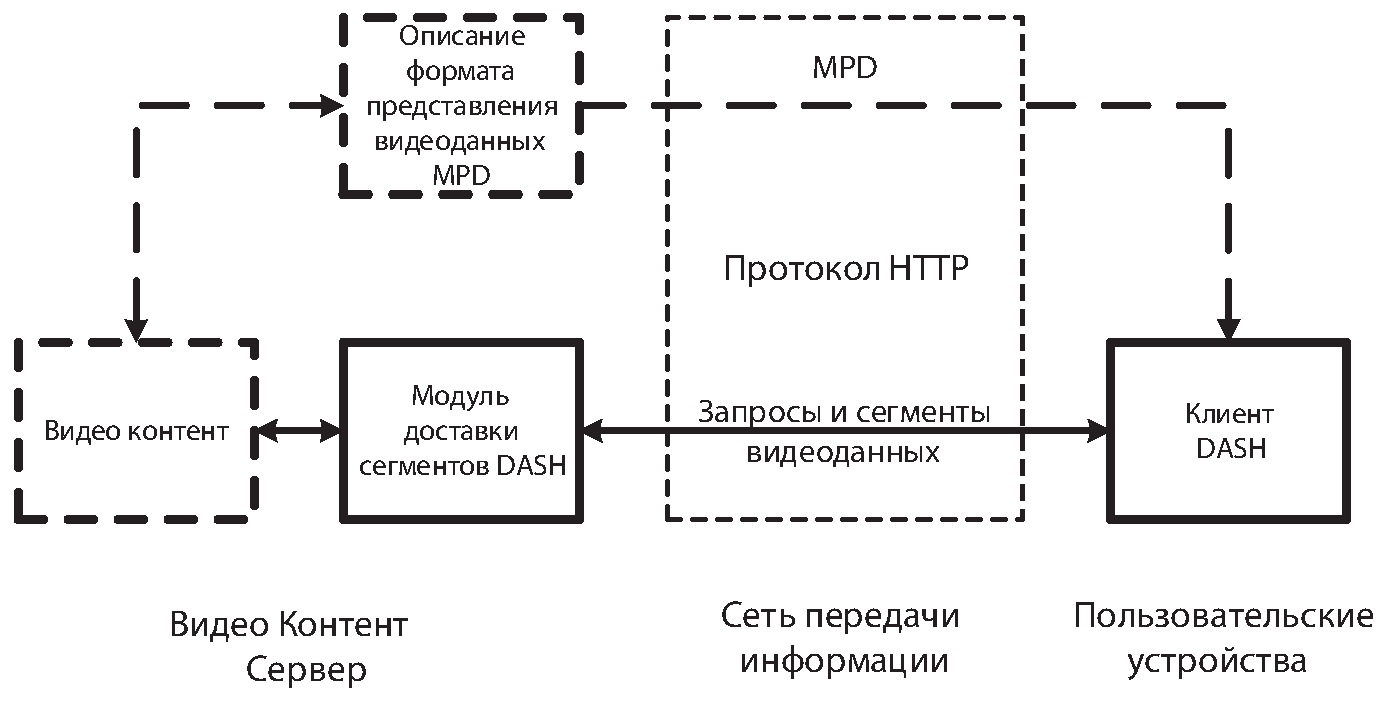
\includegraphics[width=0.8\textwidth]{Chapter1/Base_Scheme.pdf}
\caption{Обобщенная структура систем передачи видеоданных}
\label{fig:Base_Scheme}
\end{center}
\end{figure}

При передаче видеоданных удаленно в сети Интернет установлена система серверов (Видео Контент Сервер), хранящая видеоданные. К данной системе посредствам HyperText Transfer Protocol (HTTP), HyperText Transfer Protocol Secure (HTTPS) или Transport Layer Security (TLS) протоколам через сеть передачи информации подключаются пользовательские устройства. При установке соединения с каждым пользователем производится формирование сессии по протоколу гарантированной доставки данных TCP (Transmission Control Protocol). Данный протокол обеспечивает надежную передачу информации между узлами сети за счет использования дополнительных сообщений, подтверждающих доставку данных (квитанций). Важно отметить, что загрузкой видеоданных управляет программный комплекс, установленный на пользовательском устройстве~--~видеоплеер. Именно видеоплеер принимает решение о порядке загрузки данных путем формирования последовательности запросов на сервер хранения информации в зависимости от воспроизведения и статистики получения информации.

Исходя из специфики работы работы сетевых протоколов HTTP и TCP, при прохождении через сеть передачи информации происходит только задержка данных при доставке на пользовательское устройство. Как следствие, невозможна ситуация, когда происходит потеря данных при передаче через сеть. Важной особенностью систем, основанных на протоколе HTTP, является их инвариантность к сети передачи информации: для обеспечения работы такой системы необходима лишь корректная работа протокола HTTP и нижележащих уровней. Однако, использование на транспортном уровне протокола TCP вносит небольшую избыточность, обусловленную квитированием и повторными передачами данных.

Задержка при передаче информации может привести к появлению негативных эффектов воспроизведения, таких как длительное время ожидания начала проигрывания, остановка воспроизведения ввиду недостатка загруженных данных и, как следствие, уменьшению удовлетворенности пользователя просмотром.

Целью данного раздела является именно установление взаимосвязи между характеристиками сети передачи информации и удовлетворенностью пользователя проигрыванием потока, прошедшего через нее. На основе данной взаимосвязи возможно построить решения для увеличения производительности телекоммуникационных сетей для передачи видеоданных. Первым шагом для достижения поставленной цели является рассмотрения формата представления видео информации при передаче через телекоммуникационные сети.

Основные результаты данного раздела опубликованы в работе \cite{past_ius}.

\section{Представление видеоданных при передаче через телекоммуникационные сети}
\label{chap1:VideoFormat}

Опишем формат хранения информации на Видео Контент Сервере для передачи с использованием HTTP протокола. Каждая последовательность, хранящаяся в памяти сервера, разбита на периоды равной длительности называемыми сегментами (в англоязычной литературе Segments или Chunks). Каждый сегмент характеризуется уникальным идентификатором (порядковым номером и идентификатор видео) и репрезентацией~\cite{dash_standard}.

Репрезентация является общепринятой характеристикой видеопотока. Она включает в себя три параметра:
\begin{itemize}
  \item Битовая скорость потока~--~объем информации, необходимый для хранения данных в одну единицу времени. Общепринятая единица измерения битовой скорости потока Мбит/c (мегабит в секунду). В русскоязычной литературе для обозначения данного термина иногда используется термин битрейт, являющийся транскрипцией англоязычного аналога~--~Bitrate.
  \item Рекомендованное разрешение~--~количество точек экрана, занимаемое при демонстрации сегмента. Данная характеристика измеряется в прогрессивной развертке (p) плотно ассоциирована с размерами экранов воспроизводящих устройств, например, 720р определяет экран формата высокого разрешения (High Definition) с 720 точками по вертикали. Исходя из стандартного соотношения сторон экранов 16:9, определяется экран размера 1280 точек по горизонтали и 720 по вертикали.
  \item Частота кадров~--~число кадров, воспроизводимое в одну единицу времени. Общепринятой единицей измерения частоты кадров является кадр в секунду.
\end{itemize}

Важно отметить, что при передаче сегмента через сеть информация, содержащаяся в сегменте информация представляется ввиде последовательности из пакетов равного объема. В реальной системе размер пакета ограничен сверху значением максимального размера полезного блока информации одного пакета, передача которого возможна без фрагментации данных (в англоязычной литературе Maximum Transmission Unit или MTU). В сети Интернет значение MTU варьируется в отрезке от 536 до 1440 байт.

Для демонстрации взаимосвязи перечисленных выше параметров приводится таблица~\ref{tab:youtubeBr}, демонстрирующая рекомендации по настройкам репрезентации сегментов~\cite{YouTubeBR,HuaweiReport}. В данной таблице частота кадров считается Стандартной, если она не превышает 30-ти кадров в секунду, и Высокой если она превосходит данное значение.

\begin{table}[!h]
    \caption{Рекомендованные настройки репрезентации сервисом YouTube}
    \begin{center}
		\label{tab:youtubeBr}
	    \begin{tabular}{|c|c|c|c|}
		\hline
		\multirow{2}{*}{Разрешение} & \multicolumn{2}{c|}{Стационарные} & \multirow{2}{*}{Мобильные} \\
		 & \multicolumn{2}{c|}{устройства} & \multirow{2}{*}{устройства} \\
		\cline{2-3}
		 & Стандартная & Высокая & \\
		 & частота кадров & частота кадров & \\
		\hline
		2160p (4К) & 35–45 Мбит/c & 53–68 Мбит/c & 13.5 Мбит/c \\
		\hline
		1440p (2К) & 16 Мбит/c & 24 Мбит/c & 6 Мбит/c \\
		\hline
		1080p (Full HD) & 8 Мбит/c & 12 Мбит/c & 3 Мбит/c \\
		\hline
		720p (HD) & 5 Мбит/c & 7.5 Мбит/c & 1.5 Мбит/c \\
		\hline
		480p & 2.5 Мбит/c & 4 Мбит/c & 0.7 Мбит/c \\
		\hline
		360p & 1 Мбит/c & 1.5 Мбит/c & 0.45 Мбит/c \\
		\hline
		240p & - & - & 0.25 Мбит/c \\
		\hline
		\end{tabular}
	\end{center}
\end{table}

Из анализа таблицы~\ref{tab:youtubeBr} возможно вывести следующие закономерности:
\begin{enumerate}
  \item С увеличением разрешения экрана на одну позицию битовая скорость возрастает примерно в два раза;
  \item Битовая скорость видеопотока для мобильных устройств в несколько раз ниже, чем для стационарных. Данный факт обусловлен разницей между размерами экранов мобильных и стационарных устройств.
\end{enumerate}

При преобразовании исходной видеопоследовательности в формат хранения данных на контент сервере возможны два режима кодирования: с неизменяемой и изменяемой битовой скоростью потока (в англоязычной литературе Constant и Variable Bitrate соответственно). Под неизменяемой битовой скоростью потока понимается следующее: все сегменты последовательности в заданном разрешении имеют равные битовые скорости. При изменяемой битовой скорости каждый сегмент даже в одном разрешении может иметь отличные друг от друга битовые скорости. Наличие двух режимов кодирования вызвано динамичностью сцен исходной последовательности, например, статичные сцены могут быть более эффективно сжаты видеокодеком, чем динамичные, как следствие в зависимости от сложности сцен исходного видео имеется возможность уменьшить объем хранимой информации без потери качества.

На качественном уровне, наличие двух возможных режимов кодирования последовательностей затрудняет разработку решений для увеличения производительности при передаче видеоданных в телекоммуникационных сетях. Так как появляется дополнительная зависимость требований к ресурсам телекоммуникационной системы от содержания видео. На данный момент сервис YouTube поддерживает только режим с неизменяемой битовой скоростью репрезентации~\cite{YouTubeBR}.

Для описания всей имеющейся информации о видеопоследовательности был разработан специальный формат представления Media Presentation Description (MPD) файл, описывающий каждый сегмент последовательности: идентификатор, длительность и репрезентация. Файл данного формата загружается на видеоплеер перед началом загрузки видео, и на основе информации, записанной в нем, видеоплеер будет осуществлять загрузку видеопоследовательности.

После определения формата хранения и представления видеопотока необходимо ответить на вопрос: каким образом организована передача видео с Контент Сервера на пользовательское устройство. Исходя из представленной информации в подразделе~\ref{chap1:SystemStructure} следует, что ведущую роль при передаче видео исполняет видеоплеер. Как следствие, следующим шагом необходимо провести анализ существующих видеоплееров и на основе данного анализа сформировать модель трафика, генерируемого при просмотре видеоконтента.

\section{Технологии адаптивной потоковой передачи видеоданных}
\label{chap1:VideoPlayers}

Важным моментом при организации передачи видео через телекоммуникационные сети является работа воспроизводящего устройства и модель поведения пользователя.

Изначально введем модель поведения пользователя при просмотре видеоконтента (рисунок~\ref{fig:UserActivity}). В начальный момент времени пользователь не просматривает видеоданные (не активен). Через некоторый случайный промежуток времени будет начат просмотр видеоряда: дана команда видеоплееру, установленному на пользовательском устройстве, организовать передачу и демонстрацию загруженного контента с сервера хранения видео. Важно отметить, что пользователь просматривает заказанное видео полностью и считается активным в период просмотра. После окончания просмотра каждой видеопоследовательности, через случайный промежуток времени (паузу) пользователь снова начнет просматривать видео.

\begin{figure}[htbp]
\begin{center}
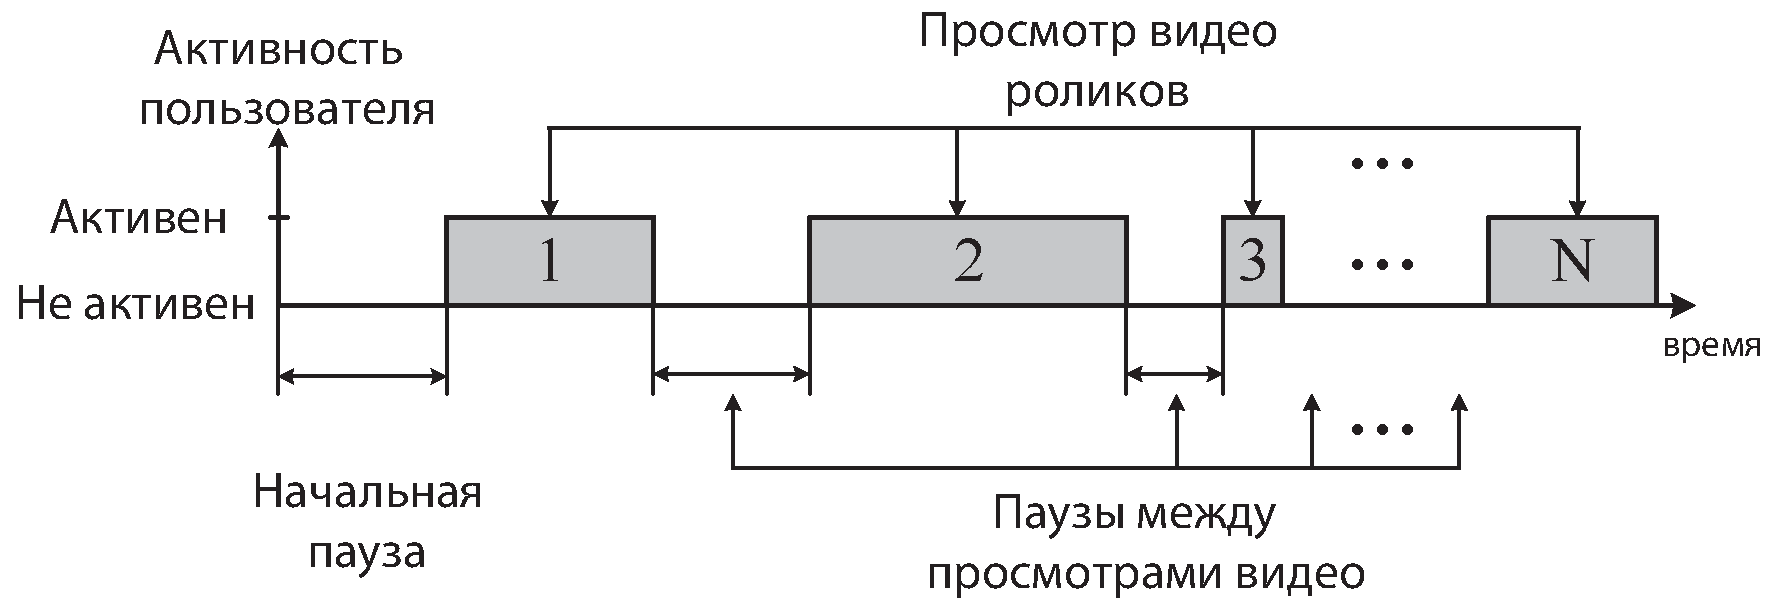
\includegraphics[width=\textwidth]{Chapter1/UserActivity.pdf}
\caption{Модель поведения пользователя при просмотре видео}
\label{fig:UserActivity}
\end{center}
\end{figure}

Описанная выше модель поведения пользователя может быть определена следующим набором случайных величин:
\begin{itemize}
  \item Длительность интервала времени перед заказом первого видео;
  \item Длительность заказанного видеоряда;
  \item Длительность пауз между просмотрами видео.
\end{itemize}

Таким образом, при наблюдении за трафиком, проходящим через сетевой (и нижележащие) уровень семиуровневой модели OSI, фиксируется чередование периодов наличия и отсутствия (пульсации) трафика у абонента. Однако, данное утверждение задает лишь обобщенную модель трафика со стороны пользователя системы передачи видеоданных. Для того чтобы окончательно определить модель генерируемого трафика необходимо рассмотреть аспекты работы видеоплеера в активный период загрузки видеопоследовательности.

В настоящие дни существует огромное множество сервисов хранения видеоданных и каждый из них представляет собственный программный комплекс, обеспечивающий загрузку видео с уникального сервиса. Исходя из данного факта провести обзор всех возможных видеоплееров не представляет возможным, поэтому в данной работе будет представлена обобщенная модель видеоплеера. Данная модель, не теряя общности, описывает все важные аспекты работы всевозможных плееров видеоданных.

На рисунке~\ref{fig:Player_avt} изображен конечный автомат видеоплеера. В начальный момент времени плеер находит в состоянии \textit{Ожидания} начала загрузки, нахождение в данном состоянии обусловлено ожиданием указаний от пользователя. После получения команды пользователя о начале загрузки будет установлено соединение с сервером хранения видеоданных и произведен переход в состояние \textit{Буферизация}.

\begin{figure}[htbp]
\begin{center}
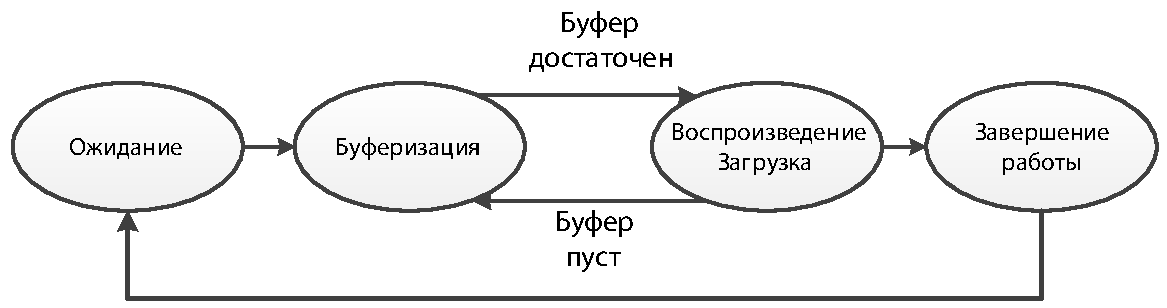
\includegraphics[width=\textwidth,height=0.2\textheight]{Chapter1/player_avt.pdf}
\caption{Конечный автомат видеоплеера}
\label{fig:Player_avt}
\end{center}
\end{figure}

В состоянии \textit{Буферизация} видеоплеер не осуществляет демонстрацию загружаемых видеоданных, а производит накопление видеоданных до определенного уровня для последующей демонстрации. Осуществление буферизации на воспроизводящем устройстве призвано уменьшить негативные эффекты воспроизведения, вызванные изменением свойств канала передачи данных, что особенно актуально для беспроводных систем передачи данных. Пребывание в данном состоянии является негативным эффектом при просмотре видео. После накопления достаточной длительности видеопоследовательности в буфере видеоплеер переходит в состояние \textit{Воспроизведение и Загрузка}.

В течении состояния \textit{Воспроизведение и Загрузка} плеер решает две важные задачи: демонстрация контента и адаптация загружаемого потока для максимизации длительности возможного времени воспроизведения. Вторая задача не является тривиальной и решается, в рассмотренных далее реализациях, эвристическими методами. Важно отметить, что в данном состоянии происходит одновременное наполнение и опустошением буфера на пользовательском устройстве, и если скорость наполнения будет меньше скорости опустошения, то в некоторый момент времени в буфере не найдется необходимого объема данных для обеспечения демонстрации. Описанное событие называется опустошение буфера, и при его наступлении видеоплеер возвращается в состояние \textit{Буферизация}, где будет находиться до накопления достаточного объема видеоданных.

В некоторый момент времени будет закончена загрузка видеоданных на пользовательское устройство. И видеоплеер осуществит переход в состояние \textit{Завершение Работы}. В данном состоянии будет закрыто соединения с сервером и ожидание окончания просмотра, после чего видеоплеер переходит в состояние \textit{Ожидания} начала загрузки.

Завершающим шагом для описания модели генерируемого трафика при просмотре видео является рассмотрение существующих методов адаптации загружаемого потока для максимизации длительности возможного времени воспроизведения в состоянии \textit{Воспроизведения и Загрузки}. Всевозможные плееры видеоданных разделяются на два множества:
\begin{itemize}
  \item HTTP Progressive Download (HPD)~--~множество плееров, не осуществляющих адаптацию видеопотока;
  \item HTTP Adaptive Streaming (HAS)~--~множество плееров, осуществляющих адаптацию видеопотока.
\end{itemize}
Для упрощения терминологии и уменьшения используемых англоязычных аббревиатур далее в работе при обозначении плееров HPD будет использоваться термин \textit{неадаптивные}, а для обозначения плееров HAS~--~\textit{адаптивные}

В начале тысячелетия в сети Интернет все видео были представлены лишь в одной репрезентации, и для их доставки использовались реализации неадаптивных плееров. Однако, даже в настоящее время неадаптивные плееры очень широко распространены. Они используются в браузере Safari для загрузки видеоданных с сервиса YouTube, для просмотра видео в социальной сети Facebook и при передаче трансляций в режиме реального времени (спортивные соревнования, прессконференций и т. д.). Как правило, для мероприятий, транслирующихся в реальном времени, не организуется кодирование видеопотока для нескольких репрезентаций, а доступна лишь одна для ознакомления с содержанием мероприятия.

Далее приведено описание работы неадаптивного плеера в состоянии \textit{Буферизация} и \textit{Воспроизведение и Загрузка}. После получения команды от пользователя о начале загрузки некоторого видео на пользовательское устройство загружается MPD файл с описанием последовательности, и пользователю предлагается выбрать репрезентацию для просмотра. На основе выбранной репрезентации будет отправлен запрос на контент сервер, который организует последовательную отправку сегментов видео на воспроизводящее устройство. Далее происходит буферизация последовательности некоторой длительности и после окончания буферизации начнется воспроизведение. Если по каким-либо причинам пользователь желает изменить репрезентацию просматриваемого видео, то на сервер будет отправлен новый запрос с ее указанием и идентификатором сегмента, с которого необходимо начать передачу видеоданных (рисунок~\ref{fig:hpd_logic}). Логика отправки запросов на контент сервер регламентируется правилом: \textit{<<запрос на новый сегмент отправляется после получения текущего загружаемого сегмента>>}.

\begin{figure}[htbp]
\begin{center}
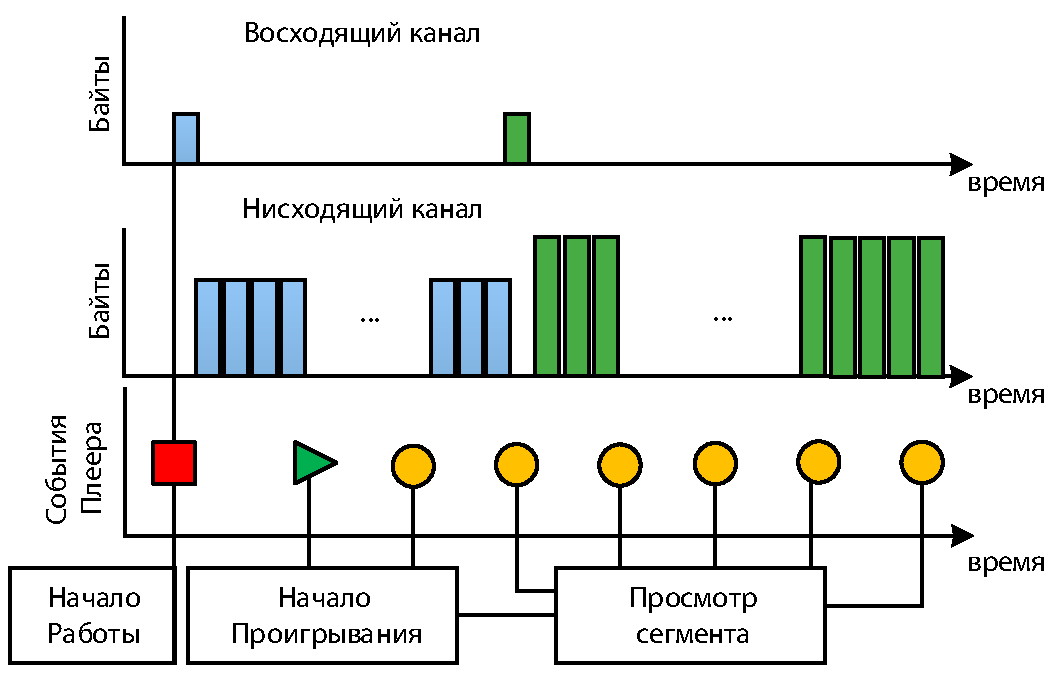
\includegraphics[width=0.7\textwidth]{Chapter1/hpd_logic.pdf}
\caption{Логика работы неадаптивного видеоплеера}
\label{fig:hpd_logic}
\end{center}
\end{figure}

Во время работы неадаптивного видеоплеера в состоянии \textit{Воспроизведение и Загрузка} на сетевом уровне наблюдается постоянный поток видеоданных в нисходящем канале (от видео сервера к пользователю), а в восходящем канале редкие запросы от воспроизводящего устройства.

Таким образом, модель генерируемого трафика при работе неадаптивного видеоплеера представляется последовательностью периодов высокой нагрузки на сеть передачи данных со случайными паузами между ними. Длительность периодов высокой нагрузки определяется только длительностью видео и выбранной репрезентацией, без учета текущей ситуации в сети. Подобная модель модель поведения значительно увеличивает нагрузку на систему передачи данных.

За последние десять лет количество обслуживаемых устройств в сетях передачи данных росло в геометрической прогрессии. И в начале первого десятилетия 21-го века стало очевидно, что существующие телекоммуникационные сети, особенно мобильные, не обладают достаточной емкостью для обеспечения достаточного качества обслуживания большого числа абонентов, одновременно просматривающих видеоконтент. Под емкостью сети понимается максимальное число пользователей, которое может одновременно находится в сети, с необходимым уровнем качества обслуживания каждого активного пользователя. Ввиду невозможности кардинального изменения существующих телекоммуникационных систем для доставки видео был разработан новый стандарт для передачи видеоданных Moving Picture Experts Group Dynamic Adaptive Streaming over HTTP (MPEG-DASH), который позволяет частично решить проблему емкости сети~\cite{dash_standard}. В настоящее время представлена версия стандарта 3GP-DASH в спецификации консорциума, разрабатывающего решения для беспроводной связи 3GPP \cite{conviva}. Стандарт 3GP-DASH включает в себя описание адаптивной и неадаптивной технологии передачи видео по протоколу HTTP.

Стандарт DASH описывает лишь формат представления видеоданных (подраздел~\ref{chap1:VideoFormat}) и общие идеи правил формирования запросов видеоплеера к серверу на сегменты видео, которые позволяют организовать адаптивную передачу видеопотока для специфичных требований каждого конкретного сервиса доставки контента. Обобщенная логика работы видеоплеера, описывающая основную идею представленную в стандарте DASH, демонстрирует рисунок~\ref{fig:has_logic}.

\begin{figure}[htbp]
\begin{center}
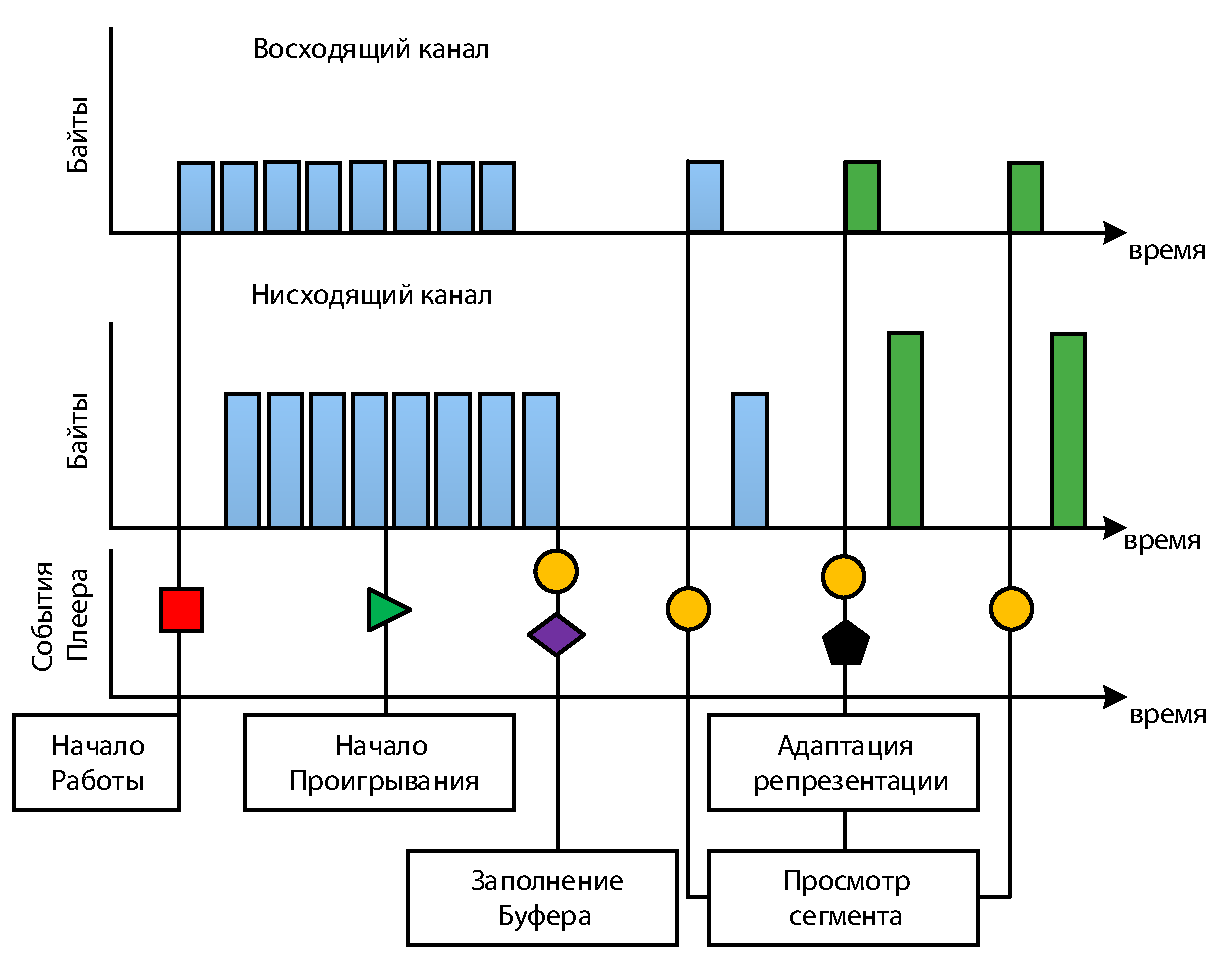
\includegraphics[width=0.7\textwidth]{Chapter1/has_logic.pdf}
\caption{Логика работы адаптивного видеоплеера}
\label{fig:has_logic}
\end{center}
\end{figure}

После установки соединения с контент сервером и загрузки MPD файла видеоплеер самостоятельно генерирует и отправляет первый запрос на видеоданные. После загрузки каждого сегмента производится оценка скорости получения данных и длительности загруженного видео, на основе которых механизм адаптации видеоряда выберет репрезентацию для следующего сегмента. В состоянии \textit{Воспроизведение и Загрузка} изменяется логика отправки запросов на сегменты данных с \textit{<<запрос на новый сегмент отправляется после \textbf{получения текущего загружаемого сегмента}>>} на \textit{<<запрос на новый сегмент отправляется после \textbf{просмотра текущего сегмента}>>}, что приводит к появлению пауз между загрузками сегментов. Наличие алгоритма изменения репрезентации и пауз между загрузками сегментов приводит к уменьшению нагрузки на телекоммуникационные сети, и, как следствие, увеличению их емкости.

Таким образом, важными отличительными особенностями адаптивного видеоплеера от неадаптивного являются:
\begin{itemize}
  \item Отправка плеером запросов на контент сервер для каждого уникального сегмента видеопоследовательности;
  \item Наличие пауз между заказами сегментов в состоянии \textit{Воспроизведение и Загрузка};
  \item Наличие алгоритма адаптации репрезентации под характеристики сети передачи данных.
\end{itemize}

Наибольший интерес из перечисленных выше особенностей представляет алгоритм адаптации репрезентации, так как он имеет непосредственное влияние на модель генерируемого трафика. Как было сказано ранее стандарт DASH не регламентирует данный алгоритм. Однако, существует реализация опорного видеоплеера, который полностью соответствует стандарту DASH. Настоящая реализация была представленна консорциумом DASH Industry Forum, который занимается продвижением настоящего стандарта и предоставляет открытую реализацию видеоплеера и серверных приложений. Данный плеер был реализован в проекте Dash.js, исходный код которого доступен на платформе разработчиков программного обеспечения GitHub~\cite{DashJS}. Плеер Dash.js полностью соответствует требованиям стандарта DASH, постоянно обновляется и дополняется при консультациях с группой экспертов, разрабатывающий данный стандарт. Далее в работе будет описана работа опорного плеера Dash.js версии 1.5. В ходе проведения исследования был проанализирован исходный код на языке JavaScript и проведен комплекс испытаний для подтверждения полученных в ходе анализа исходного кода.

Для наглядного представления результатов проведенного анализа был создан рисунок~\ref{fig:abr}, описывающий логику адаптации битовой репрезентации видеоплеером в состояниях \textit{Буферизация} и \textit{Воспроизведение и Загрузка}. Все решения алгоритма адаптации репрезентации основаны на значении параметра \textit{<<Уровень Буфера>>}~--~длительность загруженной видеопоследовательности на пользовательском устройстве в секундах, доступной для воспроизведения. Например, при значении \textit{<<Уровень Буфера>>} равном 5-ти секундам на воспроизводящем устройстве доступно к воспроизведению 5 секунд видео в текущий момент времени, и если плеер находится в состоянии \textit{Воспроизведение и Загрузка} и в течение 5-ти секунд не будет загружен ни один сегмент, то воспроизведение прекратится и плеер перейдет в состояние \textit{Буферизация}.

Плеер Dash.js является многопоточным приложением и его работа организована в трех основных потоках, одновременно исполняющихся на пользовательском устройстве: ПРОИГРЫВАНИЕ, ЗАГРУЗКА и МОНИТОРИНГ.

В начальный момент времени работы плеера доступен MPD файл с описанием каждого сегмента видеопоследовательности, и необходимо решить задачу выбора репрезентации для первого сегмента видеопоследовательности. Для решения данной задачи реализована функция подбора репрезентации по оценке скорости получения данных. Словесно данная функция может быть описана следующим образом: найти ближайшую снизу репрезентацию с битовой скоростью не превышающую оценку скорости. Она вызывается в блоках, где присутствует команда <<Запросить>>. Для первого сегмента будет подобрана репрезентация ближайшая к скорости 1 Мбит/с, отправлен запрос на сервер и запущен поток приема данных~--~ЗАГРУЗКА.

\begin{landscape}
\begin{figure}[h]
\begin{center}
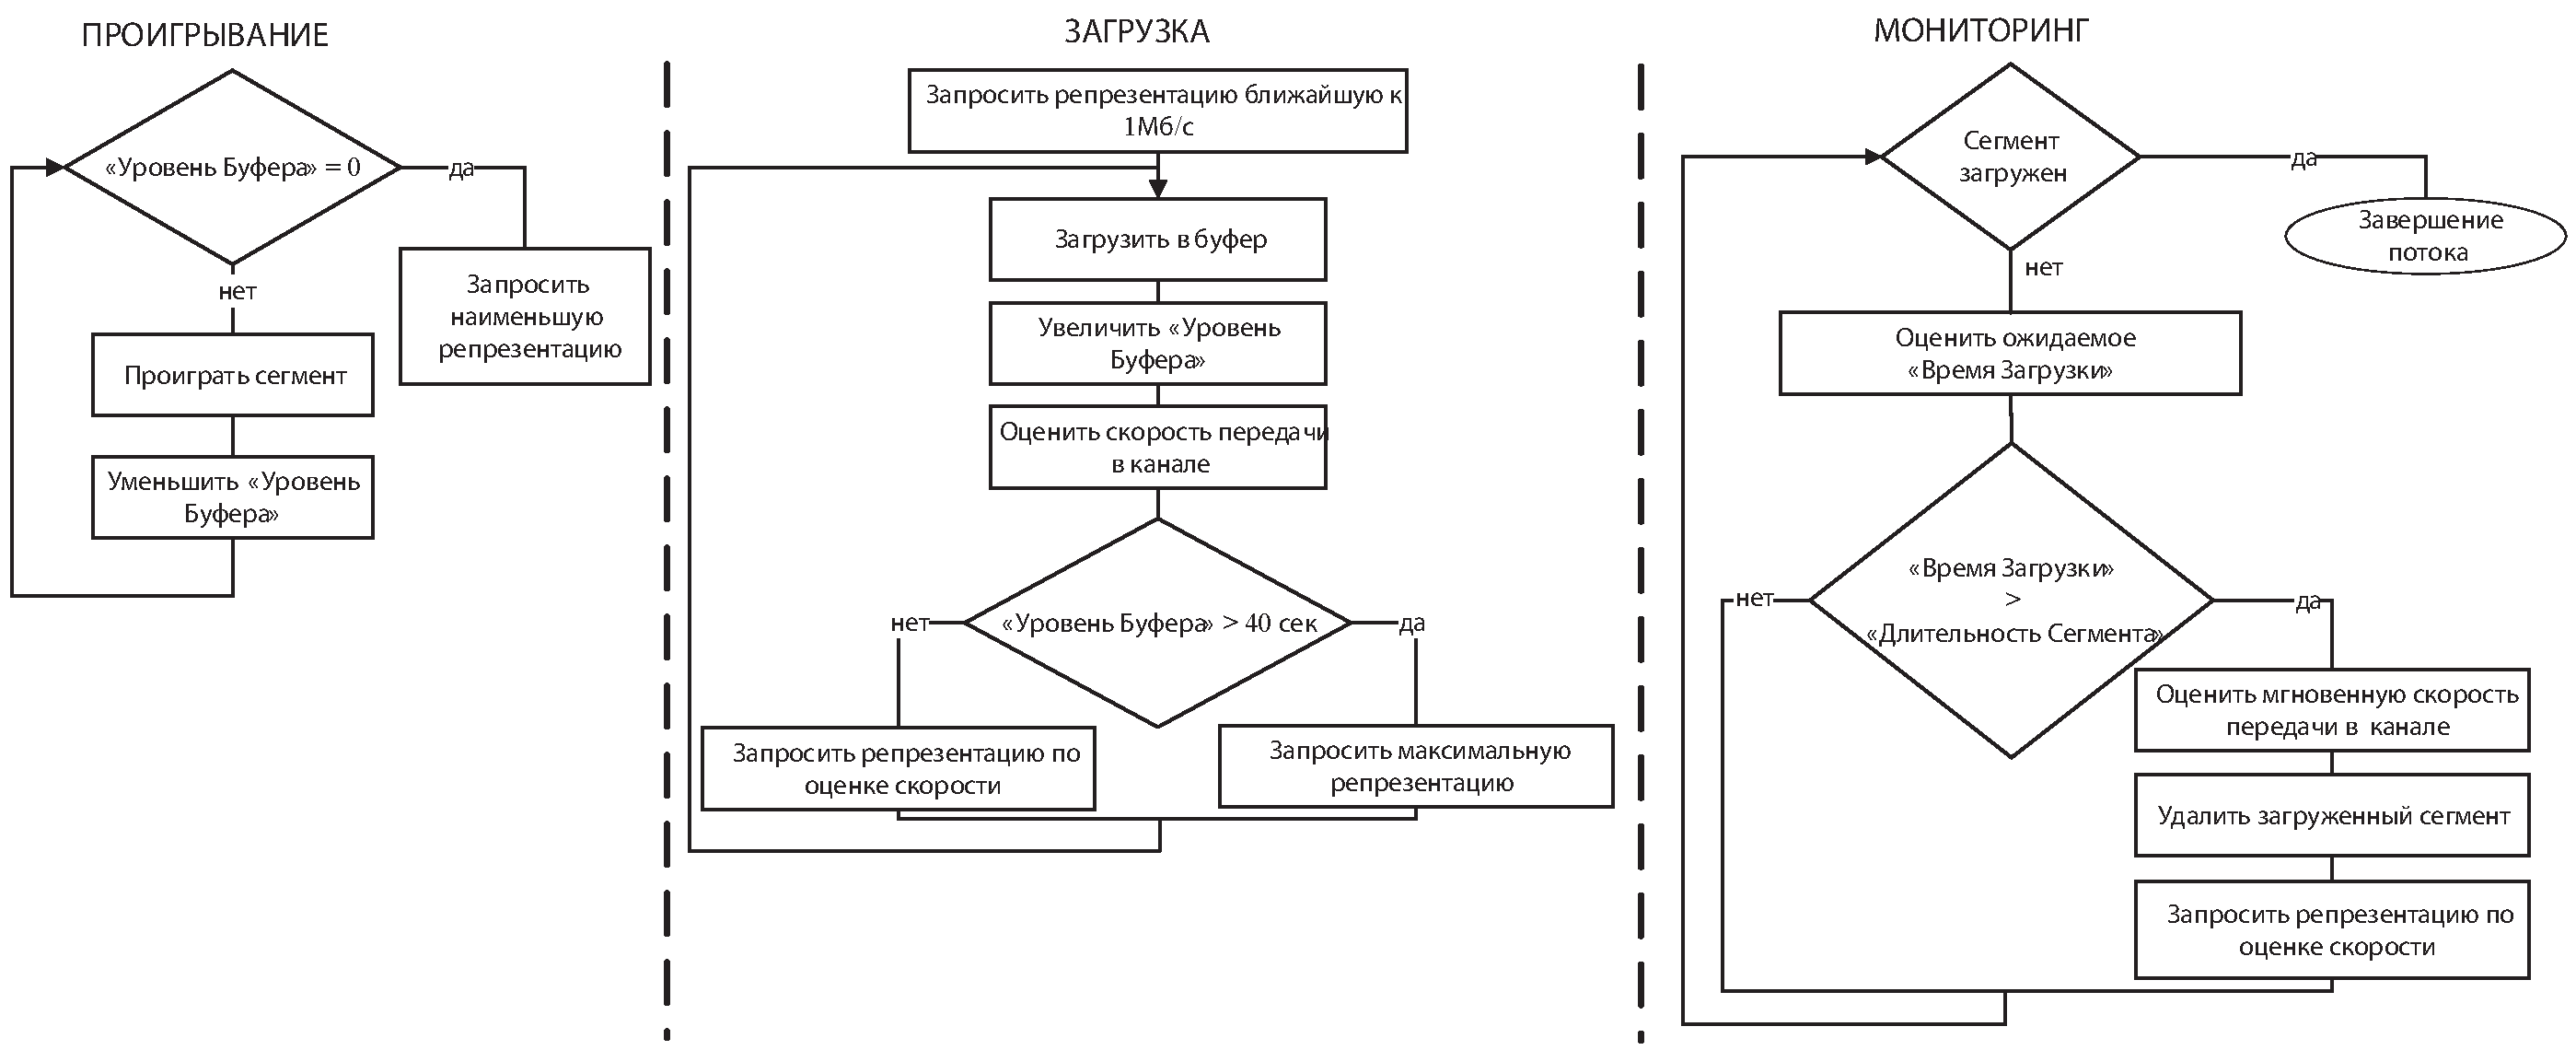
\includegraphics[width=1.5\textwidth,height=0.7\textheight]{Chapter1/abr.pdf}
\caption{Логика адаптации репрезентации опорного видеоплеера Dash.js}
\label{fig:abr}
\end{center}
\end{figure}
\end{landscape}

В потоке ЗАГРУЗКА происходит прием данных с нижележащих уровней сети, формирование сегментов видеопоследовательности и помещение их в буфер на воспроизводящем устройстве. Рассмотрим цикл загрузки одного сегмента видео. После отправки запроса на сервер в нисходящем канале начинается передача данных, и необходимо организовать их прием, контроль корректности, порядка и полноты загрузки данных. Когда сегмент будет полностью доставлен на воспроизводящее устройство он будет загружен в буфер, и значение параметра \textit{<<Уровень Буфера>>} увеличено на длительность загруженного сегмента. Далее для выбора репрезентации для следующего сегмента производится оценка скорости загрузки данных в два этапа:
\begin{enumerate}
  \item Вычисление оценки скорости загрузки текущего сегмента, как отношение размера сегмента к длительности его загрузки;
  \item Вычисление результирующей оценки скорости загрузки как среднего арифметического оценок скоростей нескольких последних сегментов и умножение полученного значения на понижающий коэффициент. Занижение результирующего значения необходимо для компенсации возможных колебаний скорости загрузки данных.
\end{enumerate}
Далее значение параметра \textit{<<Уровень Буфера>>} сравнивается с порогом достаточного уровня буфера. Если значение \textit{<<Уровень Буфера>>} выше, то следущий сегмент будет заказан в максимальной доступной репрезентации, иначе выбор репрезентации будет основан на вычисленной ранее оценке.

Одновременно с потоком ЗАГРУЗКА работает поток МОНИТОРИНГ, задачей которого является контроль длительности загрузки сегментов. Для этого в каждый момент времени загрузки происходит оценка ожидаемого времени загрузки сегмента и если данная оценка превышает произведение длительности сегмента и коэффициента порогового ожидания загрузки, то загрузка текущего сегмента будет прекращена. При прекращении загрузки все загруженные данные удаляются и в этот же момент, сервер уведомляется о прекращении загрузки сегмента и на него отправляется новый запрос с указанием репрезентации, выбранной на основе оценки скорости загрузки только текущего сегмента.

После накопления размера достаточной для начала воспроизведения длительности видео будет запущен поток ПРОИГРЫВАНИЕ, который производит демонстрацию загруженного в буфер видео. При проигрывании сегмента он изымается из буфера, и значение \textit{<<Уровень Буфера>>} уменьшается на длительность, изъятого сегмента. Данный поток влияет на выбор репрезентации только в том случае, когда уровень буфера равен нулю (в буфере нет данных для воспроизведения), тогда плеер прекращает демонстрацию видео, переходит в состояние \textit{Буферизация}, а следующий сегмент будет заказан в минимальной репрезентации.

На представленный выше алгоритм адаптации видеоряда под условия канала передачи данных налагается ограничение на частоту переключения репрезентаций видео. Очевидным является факт, что частое переключение битовых репрезентаций негативно влияет на качество восприятия видеопотока: в некоторых случаях быстрое переключение репрезентаций при просмотре приводит к проявлению симптомов неврологических расстройств. Поэтому в современных реализациях видеоплееров количество переключений в единицу времени ограничено сверху~\cite{widash}.

Основные параметры видеоплеера Dash.js были агрегированы в таблице~\ref{tab:DashJSParams}.

\begin{table}[!h]
    \caption{Основные параметры адаптивного видеоплеера Dash.js}
    \begin{center}
		\label{tab:DashJSParams}
	    \begin{tabular}{| C{4cm} | C{7cm} | C{3cm} |}
	    	\hline
	    	Название параметра & Описание & Значение \\
	    	\hline
	    	\multicolumn{3}{|c|}{Общие параметры} \\
	    	\hline
	    	Длительность сегмента видеоданных & Длительность сегментов, на которые разделена видеопоследовательность & [2, 10] секунд \\
	    	\hline
	    	Размер начальной буферизации & Длительность видеопоследовательности, которая должна быть загружена перед началом воспроизведения & 12 секунд \\
	    	\hline
	    	Максимальный размер буфера & Максимальная длительность видеопоследовательности, которая может быть помещена в буфер & 60 секунд \\
	    	\hline
	    	\multicolumn{3}{|c|}{Параметры адаптации репрезентации} \\
	    	\hline
	    	Начальная оценка канала & Оценка канала передачи данных, на основе которой будет выбрана репрезентация первого сегмента & 1 Мбит/c \\
	    	\hline
	    	<<Память>> при оценке скорости канала & Число сегментов, на основе которых будет производиться оценка скорости канала передачи данных & 3 \\
	    	\hline
	    	Понижающий коэффициент оценки скорости & Коэффициент для понижения оценки скорости передачи данных, при оценке скорости загрузки & 0.9 \\
	    	\hline
	    	Достаточный уровень буфера & Длительность буферизированного видеопотока, при котором плеер будет заказывать только максимальную репрезентацию & 40 секунд \\
	    	\hline
	    	Коэффициент порогового ожидания загрузки сегмента & Длительность числа сегментов, которых будет ожидать плеер, перед удалением текущего сегмента & 1.5 \\
	    	\hline
    	\end{tabular}
	\end{center}
\end{table}

Для адаптивного видеоплеера модель генерируемого трафика зависит как от характеристик просматриваемого видеопотока, так и системы передачи данных. Она определяется настройками видеоплеера и алгоритма адаптации репрезентации.

На текущий момент был представлен анализ организации передачи видео в телекоммуникационных сетях. Рассмотрены основные виды видеоплееров и показано влияние плеера на модель генерируемого трафика. Исходя из проведенного анализа возможно заключить, что обслуживание передачи видеоданных является нетривиальной задачей. Наиболее важным для исследования становится вопрос о влиянии характеристик сети передачи данных и видеоплеера на качество обслуживания абонента. Именно данному вопросу посвящена следующая часть раздела.

\section{Методики оценки качества передачи видеоконтента}
\label{chap1:VideoMOS}

Оценка качества передачи видеоконтента является сложной задачей ввиду субъективного восприятия пользователем характеристик воспроизведения. Существуют два основных подхода для оценки качества для всевозможных сервисов:
\begin{itemize}
  \item Экспертная оценка~\cite{Experts};
  \item Оценка пользовательского опыта использования сервиса~\cite{QoE}.
\end{itemize}

Изначально для определения качества телекоммуникационных сервисов использовались экспертные оценки. Получение подобной оценки состояло из нескольких этапов: подбор членов экспертной комиссии, формулировка строго поставленных вопросов и ожидание результата. Данная процедура занимает много времени, как следствие, использование экспертной оценки имеет смысл только уже к разработанным системам передачи данных, однако для оценки качества на этапе разработки системы использовать данный подход не представляется возможным. В настоящее время мнения экспертов используют для формирования требований к разрабатываемым стандартам связи следующего поколения.

В тоже время, наличие положительной экспертной оценки не является гарантией удовлетворенности пользователя использованием сервисом. Данный факт привел к появлению второго метода оценки качества: оценка пользовательского опыта использования сервиса, в англоязычной литературе этот термин известен как Quality of Experience (QoE). Термин QoE очень общий и включает в себя огромное число методик и критериев для различных сервисов, любой критерий с системой сравнения результатов, отражающий пользовательский опыт, считается QoE.

Для оценки качества телекоммуникационных сервисов была принята методология оценки, известная как Mean Opinion Score (MOS)~\cite{MOS_termin}. Результат оценки MOS представляется числом в отрезке от одного до пяти, где единица описывает наименьшую степень удовлетворенности пользователя, а пять наивысшую. Считается, что пользователь удовлетворен качеством сервиса, если значение MOS больше или равно трем. Для получения оценки MOS собирается статистически оправданная группа пользователей, с учетом расового, полового, возрастного и т.д. факторов, производится демонстрация сервиса, и на ее основе члены группы выставляют оценки. Результирующее значение выражается как среднее арифметическое всех даных оценок. Описанный выше путь получения оценки обладает такими же недостатками, как и экспертная оценка, однако полученный результат является более показательным, и на его основе можно организовать сравнение систем связи.

Множество усилий было направлено на ускорение получения оценки восприятия качества обслуживания, и в настоящее время для каждого вида сервисов существуют разработанные рекомендации по вычислению значения MOS. В каждой подобной рекомендации присутствует описание методологии, которая на основе огромного массива объективных характеристик доступных на пользовательском устройстве вычисляет значение оценки. Полученное значение, по утверждению авторов, не отличается от оценки, поставленной опрашиваемыми пользователями. Важно отметить следующий факт: применимость различных методологий оценки качества восприятия ограничивается типом используемого видеоплеера, например, существуют методологии, которые могут вычислить достоверное значение оценки только если при демонстрации использовался неадаптивный видеоплеер.

Организацией International Telecommunication Union, известной в РФ как Международный Союз Электросвязи, была стандартизирована процедура вычисления MOS для видеопоследовательностей с неизменяемой репрезентацией длительностью от 30-ти до 60-ти секунд~\cite{VIDEO_MOS}. Ввиду большого объема методологии, описанной в~\cite{VIDEO_MOS}, в данной работе будет представлено лишь ее описание на качественном уровне. Далее в работе для сокращения длины названий в качестве обозначения данной методологии будет называться термин ITU MOS.

Изначально на основе объективных характеристик рассчитываются два основных фактора при просмотре видео:
фактор качества видео и фактор воспроизведения~(рисунок~\ref{fig:MOS_diag}). Фактор качества видео оценивает восприятие пользователем характеристик неискаженного видеопотока на конкретном воспроизводящем устройстве. В качестве входных параметров данный фактор учитывает разрешение экрана воспроизводящего устройства, битовую скорость, частоту кадров и настройки кодирования видео и аудио потоков. Наличие, в приведенном выше списке, настроек видеокодека обусловлено влиянием алгоритма сжатия на потерю качества видеоданных. На выходе возвращается значение, нормированное в отрезке от 1-цы до 5-ти.

\begin{figure}[htbp]
\begin{center}
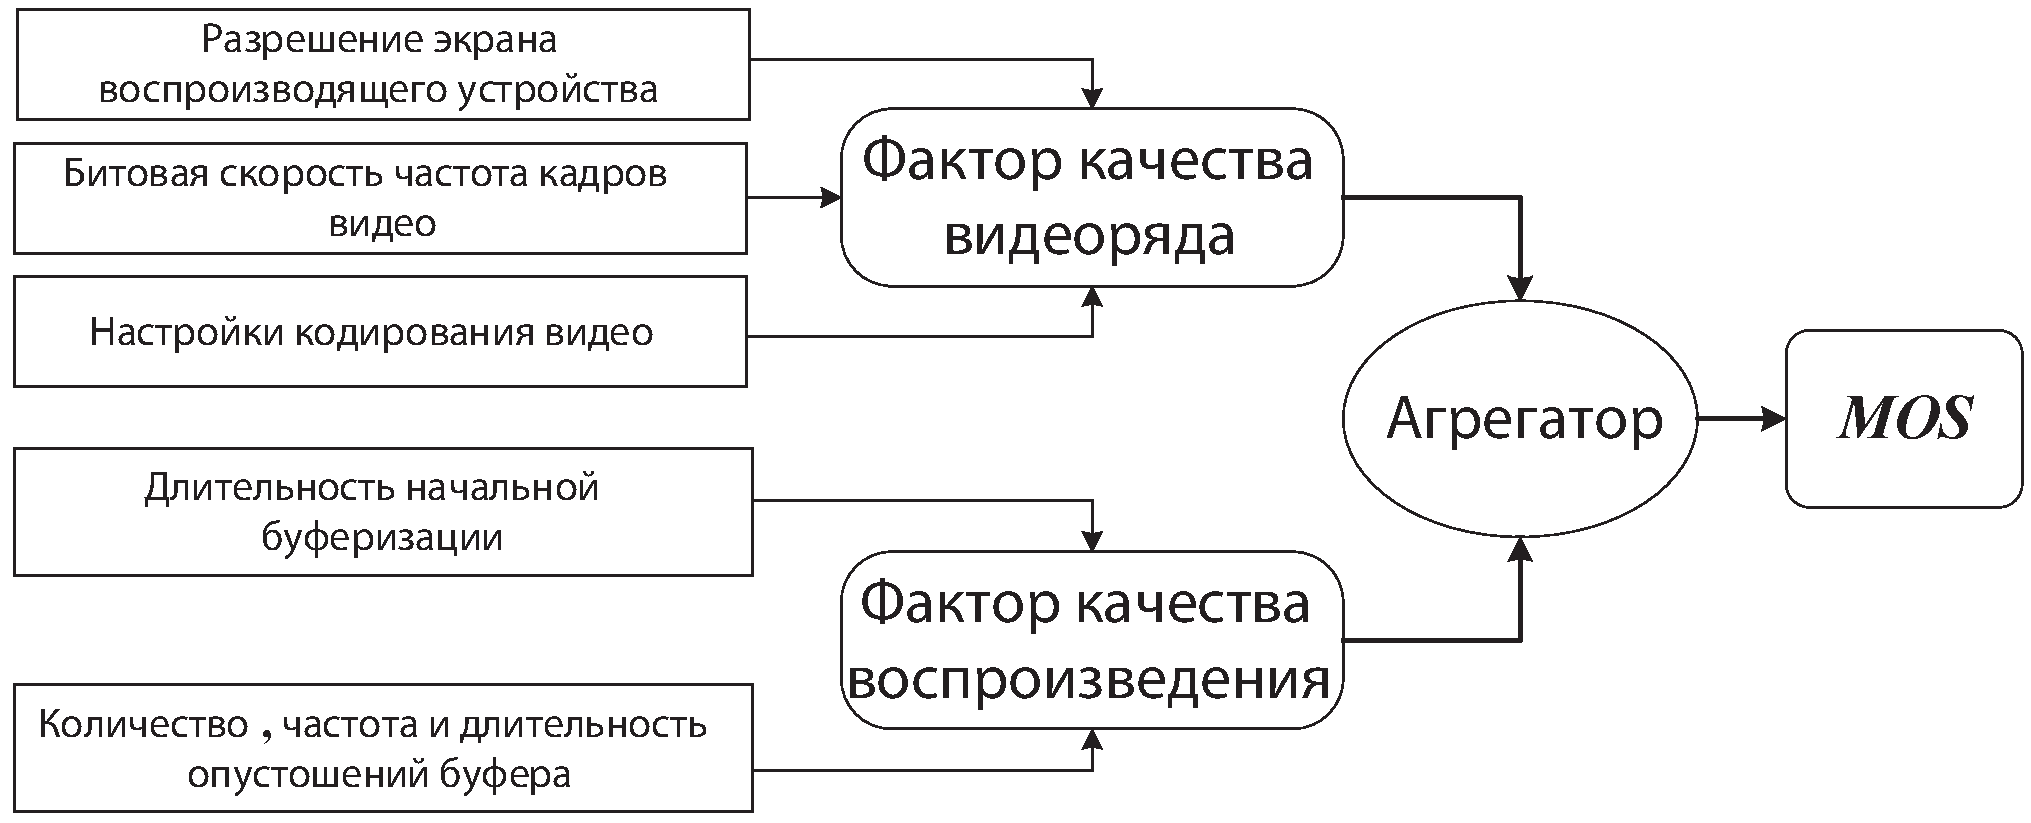
\includegraphics[width=\textwidth]{Chapter1/MOS_diag.pdf}
\caption{Схема вычисления оценки качества передачи видео в методологии ITU MOS}
\label{fig:MOS_diag}
\end{center}
\end{figure}

Фактор воспроизведения оценивает восприятие пользователем характеристик воспроизведения. Выделяются два основных негативных эффекта, имеющих определяющее влияние на оценку пользователем воспроизведение видео: начальная буферизация и опустошение буфера. Начальная буферизация характеризуется длительностью интервала времени от получения от пользователя команды о запросе видео до начала демонстрации загруженных данных (длительность нахождения в состоянии \textit{Буферизация} в начале работы видеоплеера). Считается, если длительность начальной буферизации превышает некторое значение, то пользователь откажется от просмотра.

Второй негативный эффект воспроизведения видео~--~опустошение буфера. Он характеризуется событием перехода видеоплеера из состояния \textit{Воспроизведение и Загрузка} в состояние \textit{Буферизация}, ввиду недостатка видеоданных загруженных в буфер воспроизводящего устройства. Наиболее важными в методологии ITU MOS считаются моменты времени переходов из состояний, длительности повторного нахождения в состоянии \textit{Буферизация} после осуществления начальной буферизации. Из моментов времени переходов рассчитывается частота опустошений буфера при воспроизведении видео. В методологии ITU MOS наличие хотя бы одного опустошения критично снижает оценку качества воспроизведения. На выходе фактора воспроизведения так же представляется числом от 1-цы до 5-ти.

Важным моментом работы методологии ITU MOS является метод агрегации представленных выше факторов, определяемый следующим выражением:
$$ITU MOS = max ([VideoQualityFactor - 5 + VideoPlayingFactor], 1 ),$$
где $VideoQualityFactor$~--~фактор качества видео и $VideoPlayingFactor$~--~фактор воспроизведения.

Из вида данного выражения следует, что результирующее значение MOS не может превышать оценки фактора качества видео: при идеальном воспроизведении (оценка фактора воспроизведения равна 5-ти) результирующее значение равно оценке фактора качества видео, а любое уменьшение качество воспроизведения уменьшает результат.

Основным недостатком методологии ITU MOS является его ограниченная сфера применимости, так как она может быть использована для видеопоследовательностей с неизменной битовой скоростью (неадаптивный видеоплеер) и длительностью не превышающих 60-ти секунд. Также реализация данной методологии затруднено ввиду использования огромного объема информации для вычисления оценки. В работе методология ITU MOS приведена в качестве опорного метода оценки качества восприятия видеоряда, так как все остальные методологии основаны на данной.

В настоящее время предложено несколько методологий оценки качества восприятия просмотра видео. Ярким представителем таких методологий является решение компании Huawei под названием U-vMOS (User, Unified, Ubiquitous-Mean Opinion Score for Video), которая ставит перед собой задачу оценки качества видео без ограничений на их длительность и изменение битовых скоростей. Методология Huawei U-vMOS была представлена в апреле 2016-го года на выставке London TV Connect Exhibition~\cite{UvMOSWhitePaper}.

Подробное описание данной методологии представлено в презентации на сайте компании~\cite{UvMOSPresentation}. В отличии от методологии ITU MOS, для расчета значения U-vMOS требуется намного меньшее число параметров.

Для расчета результирующей оценки качества восприятия видео по методологии U-vMOS должны быть оценены три фактора для одного сегмента видео:
\begin{itemize}
  \item Фактор качества видеоданных (sQuality);
  \item Фактор ожидания начала проигрывания (sItreraction);
  \item Фактор качества воспроизведения (sView).
\end{itemize}
Далее, для обозначения представленных факторов, будут использоваться оригинальные англоязычные термины.

Фактор sQuality описывает восприятие пользователем просмотра видеоряда некоторого разрешения на типовом экране воспроизводящего устройства. Авторами методологии U-vMOS, в качестве типовых экранов, были рассмотрены экран телевизионного устройства (42 дюйма) и экран смартфона (5.5 дюйма). Значение sQuality задано таблицой~\ref{tab:sQuality}.

\begin{table}[!h]
    \caption{Фактор качества видеоданных (sQuality) в методологии U-vMOS}
    \begin{center}
		\label{tab:sQuality}
	    \begin{tabular}{|c|c|c|}
		\hline
		\multirow{2}{*}{Разрешение} & \multicolumn{2}{c|}{Оценка} \\
		 & \multicolumn{2}{c|}{sQuality} \\
		\cline{2-3}
		репрезентации & Телевизионный & Экран\\
		 & экран & сматрфона\\
		\hline
		2880p (5K) & 4.78 & 5 \\
		\hline
		2160p (4К) & 4.65 & 4.78 \\
		\hline
		1440p (2К) & 4.2 & 4.58 \\
		\hline
		1080p (Full HD) & 4 & 4.45 \\
		\hline
		720p (HD) & 3.15 & 4 \\
		\hline
		480p & 2.44 & 3.64 \\
		\hline
		360p & 1.66 & 3 \\
		\hline
		\end{tabular}
	\end{center}
\end{table}

Фактор sInteraction описывает удовлетворенность пользователем длительностью ожидания в секундах начала воспроизведения потока и задается таблицей~\ref{tab:sIteraction}. Данная оценка является общей для всех сегментов видео и вычисляется только для первого сегмента.

\begin{table}[!h]
    \caption{Фактор ожидания начала воспроизведения (sInteraction) в методологии U-vMOS}
    \begin{center}
		\label{tab:sIteraction}
	    \begin{tabular}{| C{4cm} | C{5cm} | C{4cm} |}
	    	\hline
	    	Оценка sInteraction & \multicolumn{2}{c|}{Длительность начальной буферизации}\\
	    	\cline{2-3}
	    	& Телевизионный экран & Экран смартфона \\
	    	\hline
	    	5 & < 100 мс & < 100 мс \\
	    	\hline
			4 & 1 сек & 1 сек \\
	    	\hline
			3 & 2 сек & 3 сек \\
	    	\hline
			2 & 5 сек & 5 сек \\
	    	\hline
			1 & $\geq$ 8 сек & $\geq$ 10 сек \\
	    	\hline
    	\end{tabular}
	\end{center}
\end{table}

Важным фактором воспроизведения является sView. В качестве оцениваемой характеристики используется процент времени ожидания возобновления просмотра после события опустошения буфера к длительности сегмента видео. Оценка качества воспроизведения так же является таблично заданной функцией (таблица~\ref{tab:sView}).

\begin{table}[!h]
    \caption{Фактор качества воспроизведения (sView) в методологии U-vMOS}
    \begin{center}
		\label{tab:sView}
	    \begin{tabular}{| C{4cm} | C{5cm} | C{4cm} |}
	    	\hline
	    	Оценка sView & \multicolumn{2}{|c|}{Процент времени прерывания воспроизведения}\\
	    	\cline{2-3}
	    	& Телевизионный экран & Экран смартфона \\
	    	\hline
			5 & 0\% & 0\%\\
	    	\hline
			4 & 0.1\% & 5\%\\
	    	\hline
			3 & 1\% & 10\%\\
	    	\hline
			2 & 5\% & 15\%\\
	    	\hline
			1 & $\geq$ 10\% & $\geq$ 30\%\\
	    	\hline
    	\end{tabular}
	\end{center}
\end{table}

После того как были рассчитаны все вышеперечисленные показатели качества результирующее значение для одного сегмента может быть получено следующим образом:
$$UvMOS = (sQuality - 1)\left[\frac{\alpha(sInteraction - 1)+\beta(sView-1)}{4(\alpha+\beta)}\right] + 1,$$
где коэффициенты $\alpha$ и $\beta$ заданы таблицей~\ref{tab:Cofficients}.

\begin{table}[!h]
    \caption{Коэффициенты для расчета значение MOS в методологии U-vMOS}
    \begin{center}
		\label{tab:Cofficients}
	    \begin{tabular}{| C{4cm} | C{4cm} | C{4cm} |}
	    	\hline
	    	Коэффициент & Телевизионный экран & Экран смартфона \\
	    	\hline
			$\alpha$ & 0.66 & 0.71\\
	    	\hline
			$\beta$ & 0.77 & 0.77\\
	    	\hline
    	\end{tabular}
	\end{center}
\end{table}

Из вида функции U-vMOS следует, что если зафиксировать некоторое значение показателя sQuality, то результирующее значение не может превышать значение данного показателя. Таким образом, чтобы получить значение MOS превышающее 3, то необходимо демонстрировать пользователю видеопоток с разрешением не менее 720p и 360p для телеэкранов и смартфонов соответственно. Показатели качества sInteraction и sView, отличные от 5-ти только понижают результирующее значение MOS. Как следствие, для обеспечения значения U-vMOS больше трех следует обеспечивать более высокие репрезентации.

Компанией Huawei был представлен программный комплекс для разработчиков систем, который позволяет оценить качество воспроизведения на стороне пользовательского устройства для большинства платформ~\cite{UvMOSSdk}. Реализованный программный комплекс представлен в виде библиотеки на языке С++. Он позволяет оценить качество для адаптивного видеопотока неограниченной длительности, на основе методики U-vMOS. На вход поступают <<сырые>> данные для каждого просмотренного сегмента: разрешение, битовая скорость, прерывание воспроизведения и длительность ожидания начала воспроизведения. На выходе представлены оценки воспроизведения потока (sQuality, sInteraction, sView) и результирующее значение оценки удовлетворенности пользователя от просмотра.

Таким образом, метод оценки Huawei U-vMOS применим для адаптивного и неадаптивного видеопотока. Данное свойство позволяет использовать его для большего множества видеоконтента, по сравнению со стандартом ITU MOS. Из описания методик оценок качества воспроизведения видео ITU MOS и Huawei U-vMOS, следует что для их использования необходимо иметь доступ к информации на видеоплеере. Данное ограничение значительным образом сужает возможную сферу их применения.

Существует ряд работ, в которых ставится задача анализа и увеличения производительности существующих беспроводных систем при передаче видео, посредствам аналитического исследования функции MOS. Авторы данных работ отмечают, что описанные выше методы невозможно использовать в качестве целевых функций, ввиду большого числа параметров и их сложной, нелинейной взаимосвязи. В подобных работах рассматриваются аппроксимации MOS, которые опираются на меньшее число параметров. Так же утверждается, что оптимизация (минимизация или максимизация) таких аппроксимаций приводит к максимизации функции MOS. В таблице~\ref{tab:appraximations}~(приложение~\ref{AppA}) представлены некоторые аппроксимации, отсортированные в порядке возрастания количества используемых критериев для оценки качества обслуживания.

Таблицу~\ref{tab:appraximations} возможно использовать следующим образом: зафиксировать некоторый объем данных, доступный разработчику сети, и выбрать те критерии качества обслуживания, которые могут оценить удовлетворенность пользователя. Например, при знании битовой скорости просматриваемого потока можно использовать метод, описанный в работе~\cite{Suai2015}, однако, если добавить информацию о длительности опустошения буфера и просмотра возможна более точная оценка на основе критерия~\cite{Essaili_Rate}.

Из результатов, представленных таблицой \ref{tab:appraximations}, были сделаны следующие выводы. На удовлетворенность пользователя просмотром видео влияют два основных фактора:
\begin{itemize}
	\item Фактор качества воспроизводимого потока, определяемый разрешением и частотой кадров. На настоящий фактор оказывает непосредственное влияние битовая скорость потока (таблица \ref{tab:youtubeBr}).
	\item Фактор длительности ожидания (буферизации) в течении просмотра видеопотока.
\end{itemize}
Фактор качества воспроизводимого видео оказывает влияние на удовлетворенность пользователей, использующих адаптивную технологию передачи видеоданных, так как при использовании неадаптивной технологии качество видео выбирается самим пользователем. В свою очередь, фактор длительности ожидания в течении просмотра оказывает влияние на удовлетворенность пользователя вне зависимости от технологии передачи видео (адаптивной и неадаптивной).

Известны два критерия оценки фактора длительности ожидания, представленных в таблице \ref{tab:appraximations}:
\begin{itemize}
	\item \textit{Нормированное отношение длительностей буферизации и просмотра} \cite{QoE_Ozgur,past_tur}:
	\begin{equation}
    	\label{eq:g_def}
    	g_i = \lim\limits_{T\rightarrow\infty} \frac{b_i^T}{w_i^T + b_i^T},
    \end{equation}
    где $b_i^T$~--~общая длительность буферизации пользователя $i$ за время $T$, $w_i^T$~--~общая длительность просмотренного видео пользователем $i$ за время $T$,
	\item \textit{Отношение длительностей буферизации и просмотра} \cite{Bakin_Globecom}:
	\begin{equation}
    	\label{eq:q_def}
    	q_i = \lim\limits_{T\rightarrow\infty} \frac{b_i^T}{w_i^T}.
    \end{equation}
\end{itemize}
В настоящее время, широко исследована производительность беспроводных систем при использовании неадаптивной технологии для критерия качества (\ref{eq:q_def}), однако, для критерия (\ref{eq:g_def}) отсутствуют исследования производительности беспроводных систем связи для передачи видео по протоколу HTTP.

В последующих разделах настоящего диссертационного исследования проводится анализ производительности беспроводной системы связи для критерия качества (\ref{eq:g_def}) при использовании неадаптивной технологии передачи видео, и критерия качества (\ref{eq:q_def}) при адаптивной технологии передачи видеоданных.

После осуществления обзора различных методик оценки качества восприятия видео остается важный вопрос о взаимосвязи объективных показателей производительности сети передачи видеоданных и оценки качества восприятия (подраздел~\ref{chap1:VideoMOS}). Данному вопросу посвящена заключительная часть раздела.

\section{О взаимосвязи объективных показателей производительности сети и оценки качества восприятия видео}
\label{chap1:InterrelationKPIandQoE}

При передаче видеоданных к телекоммуникационной сети предъявляются специфичные требования, обусловленные характеристиками видеоконтента и настройками воспроизводящего устройства. Для разработчиков сетевого оборудования важно обеспечить максимально возможную емкость сети передачи данных, что ставит задачу оценки качества восприятия контента пользователем на основе некоторого объема информации. При разработке или модернизации сетей передачи данных разработчикам доступен ограниченный набор показателей качества обслуживания, который может быть с достаточной точностью оценен на физическом, канальном, сетевом и транспортном уровнях. Однако, показатели работы воспроизводящего устройства, которые имеют наибольшее влияние на удовлетворенность пользователя при просмотре видео, недоступны ввиду шифрования трафика, что делает невозможным получение данной информации на нижележащих уровнях сети.

Вопрос о взаимосвязи характеристик сети и качества обслуживания абонентов прорабатывался в большом количестве работ. Авторы подобных работ представляют список объективных характеристик (в англоязычной литературе обозначается как Key Performance Indicators или сокращенно KPI) сети и указывают их значения, для того чтобы пользователь был удовлетворен качеством обслуживания. В настоящее время современные телекоммуникационные сети и воспроизводящие устройства бурно развиваются, приведенные в данных работах количественные значения показателей изменяются в зависимости от момента написания работ. Однако, список объективных показателей качества обслуживания видеотрафика был неизменным.

На основе анализа работ~\cite{Chen,Cacheda2007,HuaweiReport} был выделен следующий список объективных показателей качества обслуживания пользователя, имеющих наибольшее влияние на передачу видео:
\begin{itemize}
  \item \textit{Задержка}~--~интервал времени от момента отправки пакета передающей стороной и до момента получения подтверждения от приемной стороны о получении пакета. В англоязычной литературе для обозначения данного вида задержки используется термин \textit{Round Trip Time}, в русскоязычной двусторонняя.

  В реальной системе задержка является случайной величиной. Как следствие, во всех работах в качестве количественного показателя приводится оценка математического ожидания данной случайной величины. Кроме математического ожидания задержку так же характеризуют параметром, который в англоязычной литературе называют Packet Delay Variation~\cite{Jitter}. Достаточно часто как в русскоязычной, так и англоязычной литературе данный параметр называют джиттером (Jitter).
  \item \textit{Джиттер}~--~оценка колебаний задержки. В рекомендации~\cite{Jitter} описывается несколько возможных видов данного параметра, далее в работе будет рассматриваться двухточечный джиттер. Двухточечный джиттер для одного пакета принимается равным значению разности между односторонней задержкой, измеренной для данного пакета, и некоторым эталонным значением задержки. Иногда эталонное значение задержки принимают равным минимальному значению, измененному за продолжительное время. В настоящее время влияние джиттер на производительность систем передачи данных нивелировано за счет введения на узлах сети буферов для сглаживания возможных колебаний задержки.
  \item \textit{Время отклика}~--~интервал времени, необходимый для организации соединения между приемной и передающей стороной. В некоторых работах данный показатель называется начальной задержкой.
  \item \textit{Скорость загрузки данных}~--~скорость передачи данных в сети.
\end{itemize}

После определении ключевых показателей производительности сети передачи данных и критериев качества восприятия видео пользователем возникает актуальный вопрос о их взаимосвязи. Данный вопрос является основополагающим для реализации методов увеличения производительности телекоммуникационных сетей для передачи видеоконтента.

Для разработчика сетей передачи данных может быть доступна информация с сетевого, транспортного, канального и физического уровней, в зависимости от вида и доступных механизмов анализа системы. Список доступной информации совпадает со списком, представленным ранее в настоящем подразделе, и он является очень ограниченным. Однако, исходя из описания критериев качества восприятия видео (подраздел~\ref{chap1:VideoMOS}), для точной оценки качества необходима информация, доступная только на уровне приложения. И подобный список ограничивается тремя позициями:
\begin{itemize}
  \item Битовая скорость и разрешение (репрезентация) воспроизводимого потока в текущий момент времени;
  \item Длительность начальной буферизации для текущего воспроизводимого видео;
  \item Статистика опустошений буфера на пользовательском устройстве.
\end{itemize}
Обладание данной информацией для каждого активного пользователя в сети и сегмента, просматриваемого им видео позволяет, в перспективе позволяет сформировать оптимальное управление системой передачи данных для увеличения ее производительности.

На практике все характеристики сети, такие как задержка, джиттер и т.д., агрегируются в полезную скорость передачи данных для каждого пользователя. Полезная скорость~--~это скорость получения данных на уровне приложения без учета накладных расходов на передачу данных (заголовки, квитанции и повторные передачи протоколов транспортного уровня). При наличии ограниченного ресурса, грамотное перераспределение полезной скорости передачи данных между активными пользователями может увеличить производительность системы в целом. Полезная скорость может быть с достаточной точностью оценена на промежуточных узлах сети как отношение объема данных, прошедшего в нисходящем канале, к длительности его доставки. Данная оценка может быть улучшена за счет анализа служебных сообщений протоколов транспортного уровня. Наиболее важным является существование эффективных механизмов управления полезной скоростью передачи данных, например, в проводных сетях возможно вносить задержку в доставку пакетов пользователю для ее ограничения сверху, а в беспроводных влиять на распределение частотно-временных ресурсов радиоканала.

Полезная скорость передачи данных имеет огромное влияние на работу всех видов видеоплееров (подраздел~\ref{chap1:VideoPlayers}). Для неадаптивного видеоплеера это выражается в длительности начальной буферизации и прерываниях воспроизведения из-за опустошения буфера, а в адаптивном плеере дополнительно на основе оценки скорости получения данных принимается решение о выборе репрезентации для сегментов видео. Все эти факторы имеют непосредственное влияние на качество восприятия видео, и, как следствие, на производительность сети.

Таким образом, основным элементом управления телекоммуникационной системой при доставке видео является полезная скорость передачи данных и существуют механизмы реализации управления передачей данных.

В исследовании передачи видеоданных по протоколу DASH \cite{HuaweiReport} для методологии оценки качества восприятия Huawei U-vMOS представлена взаимосвязь между объективными критериями качества обслуживания и субъективной оценкой качества восприятия (таблица~\ref{tab:BoundValues}). Таким образом для данной методологии существует взаимо-однозначное отображение объективных показателей обслуживания и субъективной оценки качества восприятия видеопотока. Более того, опираясь на таблицу~\ref{tab:BoundValues}, возможно осуществить оценку качества восприятия на промежуточных узлах сети для методологии Huawei U-vMOS.

\begin{table}[!h]
    \caption{Влияние объективных показателей качества обслуживания при передачи видео на критерий качества восприятия U-vMOS}
    \begin{center}
		\label{tab:BoundValues}
	    \begin{tabular}{| C{2cm} | C{2cm} | C{3cm} | C{2cm} | C{3cm} | C{3cm} |}
	    	\hline
	    	Значение & \multicolumn{5}{|c|}{Объективные показатели}\\
	    	\cline{2-6}
	    	U-vMOS & \multicolumn{2}{|c|}{Уровень приложения} & \multicolumn{3}{c|}{Промежуточные узлы}\\
	    	\cline{2-6}
	    	& Разрешение видео & Длительность начальной буферизации & Задержка & Скорость загрузки при начальной буферизации & Скорость загрузки при воспроизведении \\
	    	\hline
	    	3.0 & 720p & 3.5 с & 80 мс & 5 Мбит/с & 2 Мбит/с\\
	    	\hline
	    	3.3 & 720p & 1.5 с & 80 мс & 7 Мбит/с & 2 Мбит/с\\
	    	\hline
	    	\multirow{2}{*}{4.0} & 1080p & 1 с & 40 мс & 13 Мбит/с & 5 Мбит/с\\
	    	\cline{2-6}
	    	& 2K & 1.6 с & 40 мс & 11.7 Мбит/с & 8 Мбит/с \\
	    	\hline
	    	4.5 & 4K & 1 с & 10 мс & 32 Мбит/с & 18 Мбит/с\\
	    	\hline
    	\end{tabular}
	\end{center}
\end{table}

Из представленной выше таблицы следуют следующие выводы:
\begin{itemize}
	\item На оценку качества восприятия влияют два периода при просмотре видео: начальная буферизация и воспроизведение;
	\item Скорость загрузки данных при начальной буферизации должна быть значительно выше, чем при воспроизведении для обеспечения требуемого значения U-vMOS. Данное явление объясняется критическим влиянием длительности начальной буферизации при расчете значения U-vMOS (подраздел~\ref{chap1:VideoMOS}), и необходимостью ее минимизации.
	\item Наибольшее влияние на качество восприятия имеет полезная скорость загрузки данных.
\end{itemize}

Продолжим рассмотрение качества восприятия Huawei U-vMOS, описанного в подразделе~\ref{chap1:VideoMOS}, при использовании адаптивного видеоплеера для мобильных устройств. Покажем, каким образом управление полезной скоростью получения данных влияет на качество восприятия видео. Зафиксируем длительность начальной буферизации для видео равной 2-м секундам (sInteraction) и построим плоскость всевозможных значений критерия U-vMOS. Исходя из описания методологии, для получения оценки, требуется информация о разрешении видеопотока (sQuality) и процента времени прерывания воспроизведения (sView). Для получения оценки sQuality используем значения из таблицы~\ref{tab:youtubeBr} о взаимосвязи между битовой скоростью потока и его разрешением для мобильных устройств, а в качестве оценочного значения выберем среднее значение. Для получения промежуточных значений для битовой скорости и всех таблично заданных функций показателей качества U-vMOS был использован метод кусочной интерполяции кубическим полиномами на отрезках (Piecewise Cubic Hermite Interpolating Polynomial (PCHIP)). Полученный результат представлен на рисунке~\ref{fig:UvMOSDepending}.

\begin{figure}[htbp]
\begin{center}
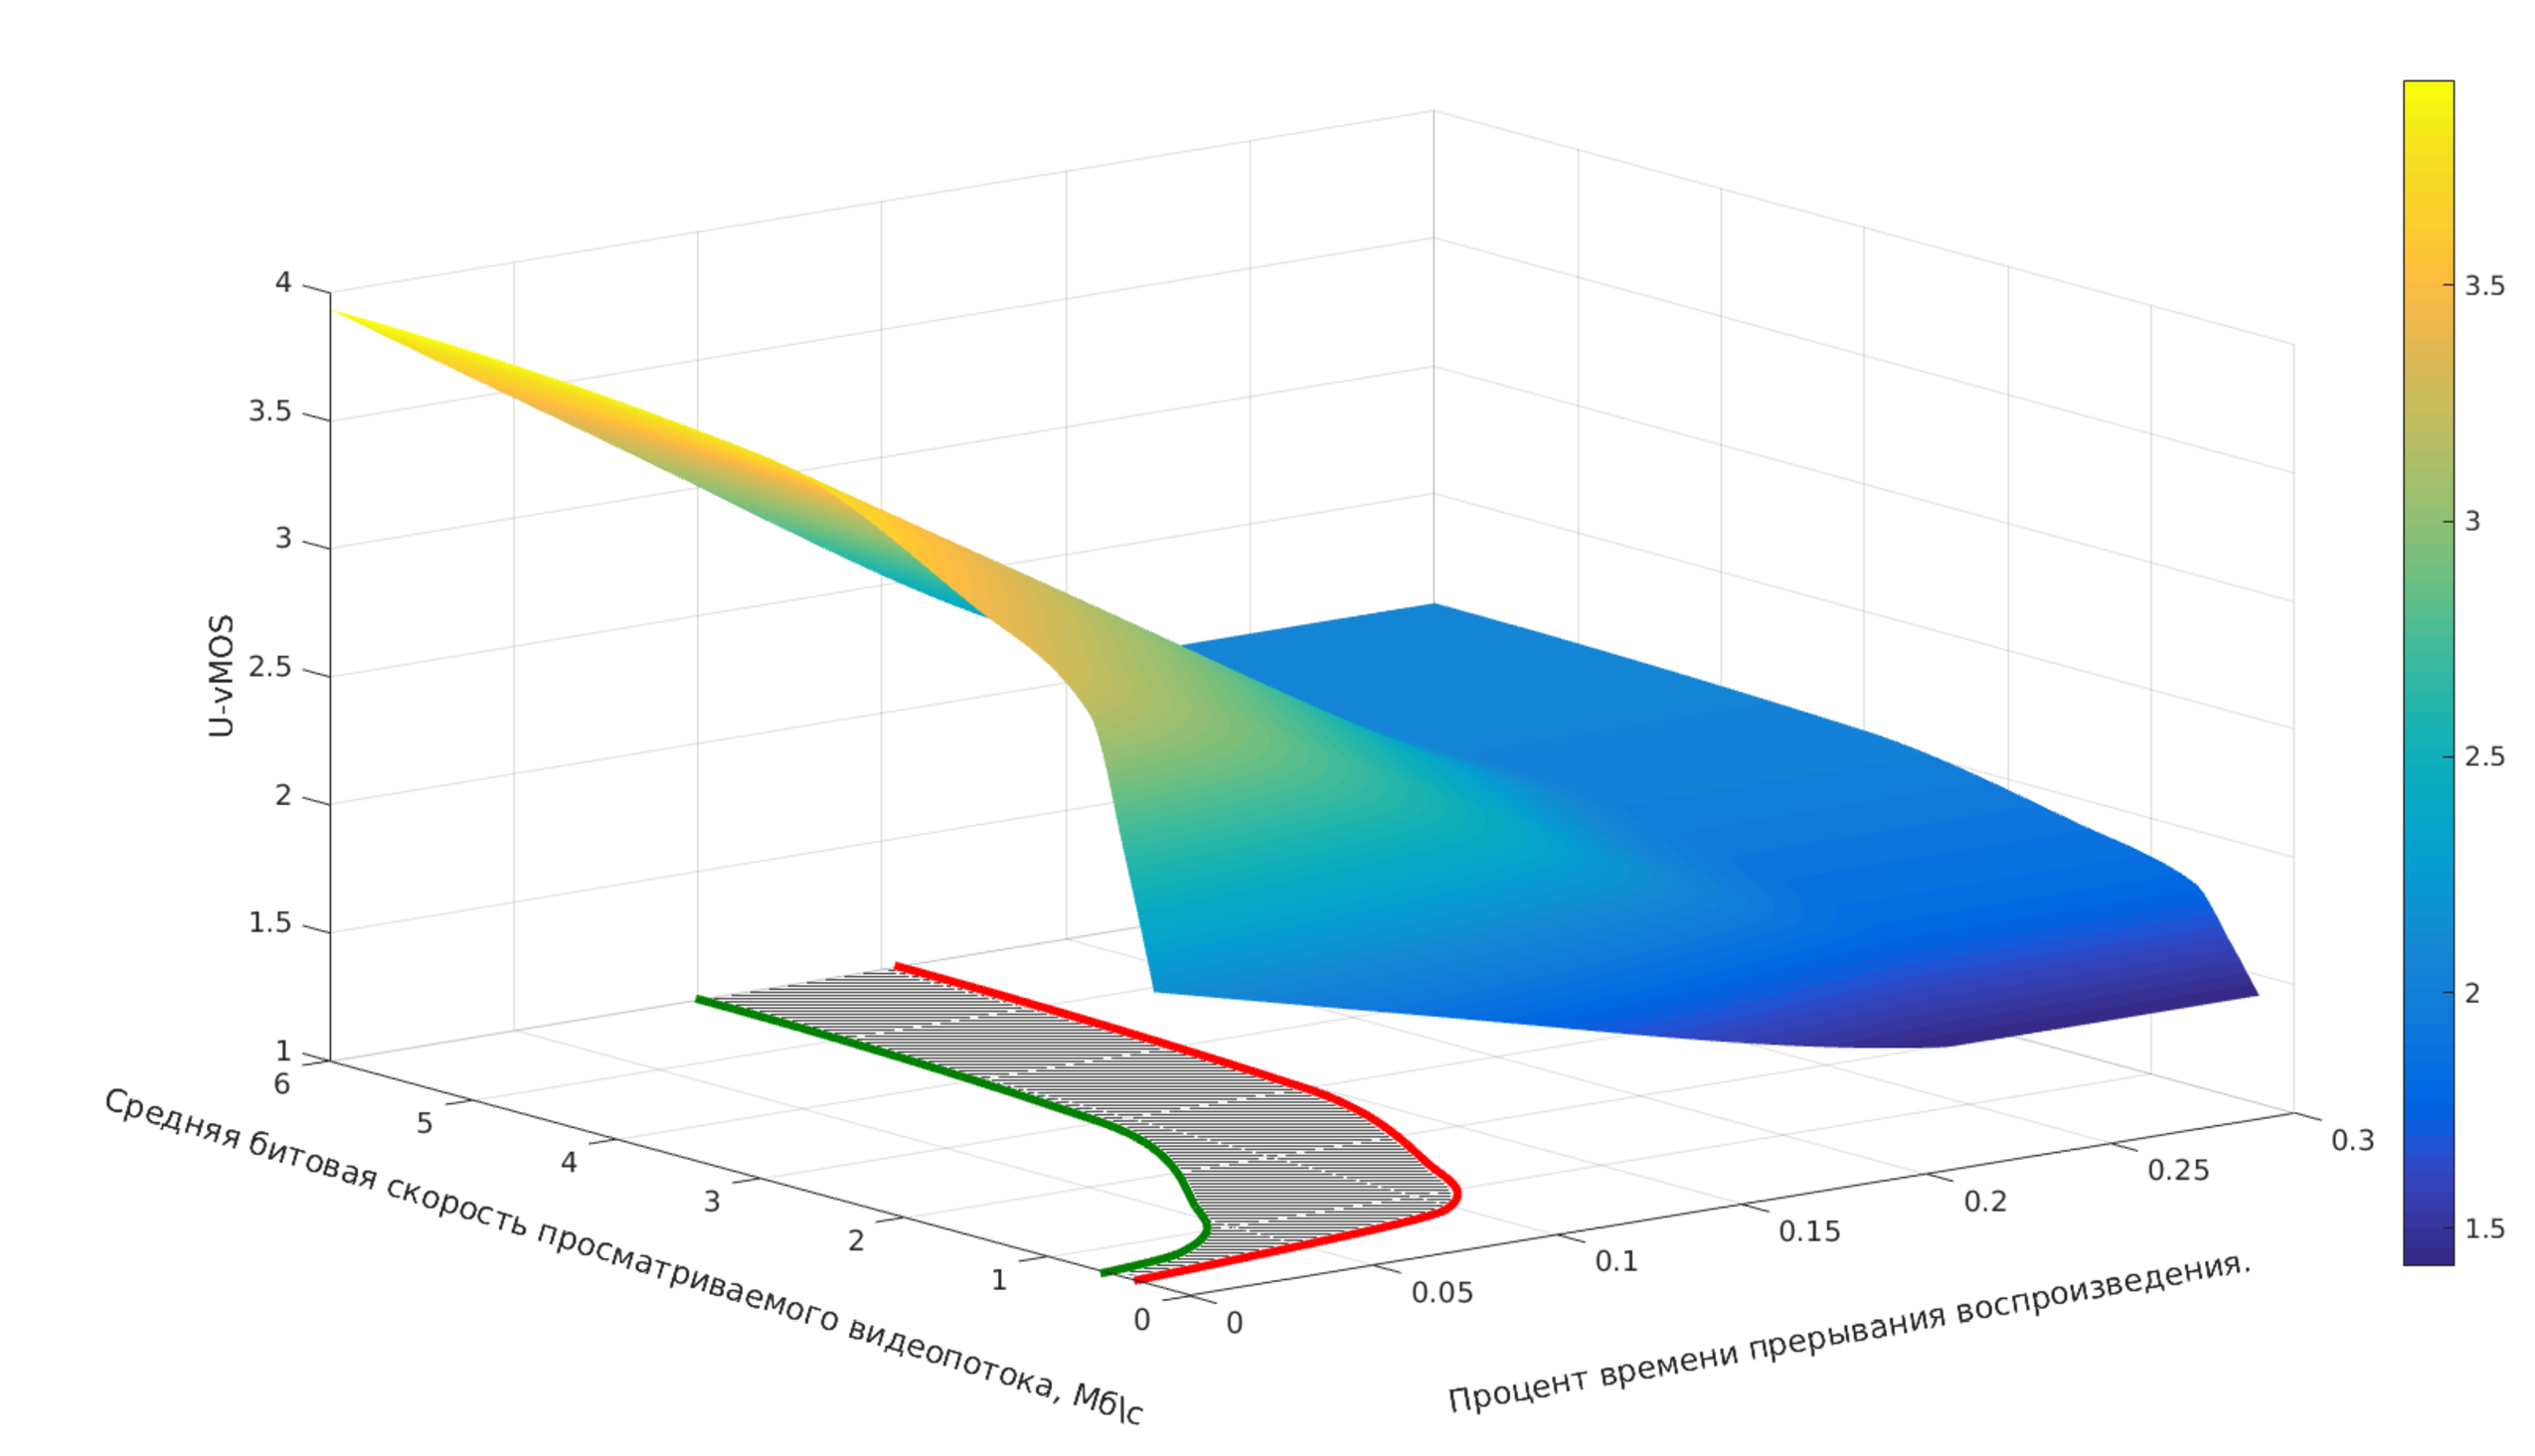
\includegraphics[width=\textwidth]{Chapter1/mos_figure.pdf}
\caption{Влияние объективных характеристик на критерий качества восприятия U-vMOS}
\label{fig:UvMOSDepending}
\end{center}
\end{figure}

По оси абсцисс отложена средняя битовая скорость просматриваемого видео, по оси ординат средний процент времени прерывания воспроизведения видео (повторные буферизации) и ось аппликат представляет результат вычисления критерия качества восприятия U-vMOS, при заданных параметрах. Процесс управлением полезной скорость передачи данных, во время просмотра видео, может привести в одну из возможных точек полученной плоскости. Значения по оси аппликат находятся в диапазоне от одного до четырех, разделим плоскость на три области:
\begin{itemize}
  \item Область высокого значения критерия восприятия (левее заштрихованной области) соответствует значениям в выше 3-х. Если пользователю была обеспечена полезная скорость для попадания в данную область, то он будет удовлетворен качеством обслуживания.
  \item Граничная область (заштрихованная область) соответствует значениям в отрезке от 2.5 до 3-х. Граничная область характеризует пограничное состояние удовлетворенности пользователя.
  \item Область низкого значения критерия восприятия (правее заштрихованной области) соответствует значениям в ниже 2.5. В данной области полезной скорости недостаточно для обеспечения достойного уровня обслуживания, таким образом пользователь считается неудовлетворенным.
\end{itemize}

Целью управления, увеличивающего производительность телекоммуникационной сети, является максимизация чила пользователей, находящихся в области высокого значения критерия восприятия. Это может быть достигнуто путем перераспределения ресурсов системы для пользователей в граничной области, за счет пользователей в области низкого значения критерия, так как перераспределение ресурсов для них не может привести к увеличению их удовлетворенности. Подобный анализ может быть проведен для любого критерия качества восприятия, представленего в подразделе~\ref{chap1:VideoMOS}.

\section{Выводы по разделу}

В качестве выводов по разделу можно отметить, что задача анализа и увеличения производительности телекоммуникационных сетей для передачи видеоданных является актуальной, ввиду бурного развития мобильных устройств. Основной целью увеличения производительности сетей является максимизация числа видеопользователей, одновременно активных в сети. Данная цель может быть достигнута путем введения управления полезной скоростью передачи данных, которое основывается на знании о формате представления видеоданных при передаче (подраздел~\ref{chap1:VideoFormat}), особенностей организации передачи видео и типах воспроизводящих устройств (подраздел~\ref{chap1:VideoPlayers}), объективных, субъективных показателей качества обслуживания и их взаимосвязи (подразделы~\ref{chap1:VideoMOS} и~\ref{chap1:InterrelationKPIandQoE} соотвественно).

Увеличение производительности телекоммуникационных систем для передачи видеоконтента является особенно актуальным для мобильных сетей связи, ввиду ограниченности ресурсов и динамичности состояния беспроводного канала.

В качестве основных результатов стоит отметить следующие:
\begin{itemize}
	\item В настоящее время существуют две технологии доставки видеоданных по протоколу HTTP: неадаптивная и адаптивная (подраздел \ref{chap1:VideoPlayers});
	\item Оценка качества восприятия видеоданных является сложной задачей ввиду субъективности пользователя, и более того зависит от технологии передачи видео (подраздел \ref{chap1:VideoMOS});
	\item Основные факторы, влияющие на качество восприятия видеопотока в зависимости от технологии передачи (подраздел \ref{chap1:InterrelationKPIandQoE}):
	\newline\textbf{Неадаптивная технология}~--~длительность буферизации в период просмотра видео;
	\newline\textbf{Адаптивная технология}~--~длительность буферизации и битовая скорость просматриваемого потока.
\end{itemize}

Информация, представленная в данном разделе, во многом носит обзорный характер, с использованием методов обратной разработки и анализа <<черного ящика>>. Представленное исследование демонстрирует основную проблематику передачи видео в телекоммуникационных системах и является основополагающим для последующих разделов работы.           % Раздел 1
\chapter{ВЗАИМОСВЯЗЬ ХАРАКТЕРИСТИК БЕСПРОВОДНОЙ ЦЕНТРАЛИЗОВАННОЙ СЕТИ И ВОСПРОИЗВЕДЕНИЯ ВИДЕОДАННЫХ}
\label{chap2}

\section{Вводные замечания}
\label{chap2:Intro}

Задача увеличения производительности при передаче видеоданных наиболее актуальна для беспроводных систем связи по причине наличия ограничений на пропускную способность радиоканала, который считается <<узким местом>> (адаптированный перевод англоязычного термина <<bottle neck>>) сети в целом. Как следствие, скорость передачи данных от видеосервера до пользовательского устройства определяется именно скоростью передачи данных по радиоканалу. Основная проблематика всех исследований в области передачи видеоданных состоит не в предложении методов управления для телекоммуникационных сетей, а в обосновании их эффективности. Однако, в настоящее время не существует опорных теоретических исследований, с которыми возможно сравнить производительность предлагаемых решений.

В настоящее время наиболее распространены централизованные беспроводные системы связи с коммутацией пакетов, так как подобные системы позволяют добиться больших скоростей передачи данных и меньших задержек в беспроводном канале связи. Наиболее ярким представителем данного класса систем является стандарт The Long-Term Evolution (LTE)~\cite{opac-b1130916}.

Настоящий раздел посвящен задаче передачи видеоданных в современных централизованных беспроводных сетях. В разделе рассматривается специфика построения современных мобильных сетей связи, и решается задача формирования аналитической модели для проведения исследований подобных систем при передаче видеоданных. Предлагаемая модель состоит нескольких вложенных моделей, описание который последовательно будет представлено в настоящем разделе. В заключении раздела предлагается основополагающий результат, описывающий взаимосвязь между характеристиками сети, которые влияют на ее производительность.

Основные результаты данного раздела опубликованы в работе \cite{past_poly}.

\section{Структура современных беспроводных централизованных сетей передачи данных}
\label{chap2:WirelessSystemStructure}

В настоящее время наибольшее распространение получили централизованные мобильные сети с коммутацией пакетов, так как они обеспечивают наиболее высокие скорости и малую задержку при передаче данных~\cite{Cisco}. В централизованных беспроводных сетях вся территория обслуживания разделена на зоны, называемые сотами. В каждой соте установлено устройство, управляющее передачей данных всех активных пользователей в зоне его ответственности, называемое Базовой станцией. Базовая станция является программно-аппаратным комплексом, обеспечивающим обмен данными между пользователем в радиосети и остальной сетью.

Современные беспроводные централизованные системы связи состоят из трех основных компонентов (рисунок~\ref{fig:LteStructure}):
\begin{itemize}
  \item \textit{Фиксированная магистральная сеть передачи данных}. Сеть передачи данных, в которая обеспечивает соединение с удаленными устройствами (в системах передачи видеоданных таким устройством является Видеосервер). Она характеризуется высокой надежностью, большой скоростью передачи данных, низкими задержкой и джиттером.
  \item \textit{Опорная сеть оператора}. Система устройств, обеспечивающая взаимодействие пользовательского устройства с удаленными узлами в фиксированной магистральной сети. Данный участок сети обладает схожими характеристиками с магистральной сетью.
  \item \textit{Радиосеть}. Беспроводная сеть передачи данных, организующая обмен данными между пользовательскими устройствами и остальными компонентами сети. Характеризуется несравнимо меньшими скоростями передачи данных и пропускными способностями каналов, большими задержкой и джиттером. Важной отличительной особенностью радиосети является изменяемость характеристик беспроводного канала во времени.
\end{itemize}

\begin{figure}[htbp]
\begin{center}
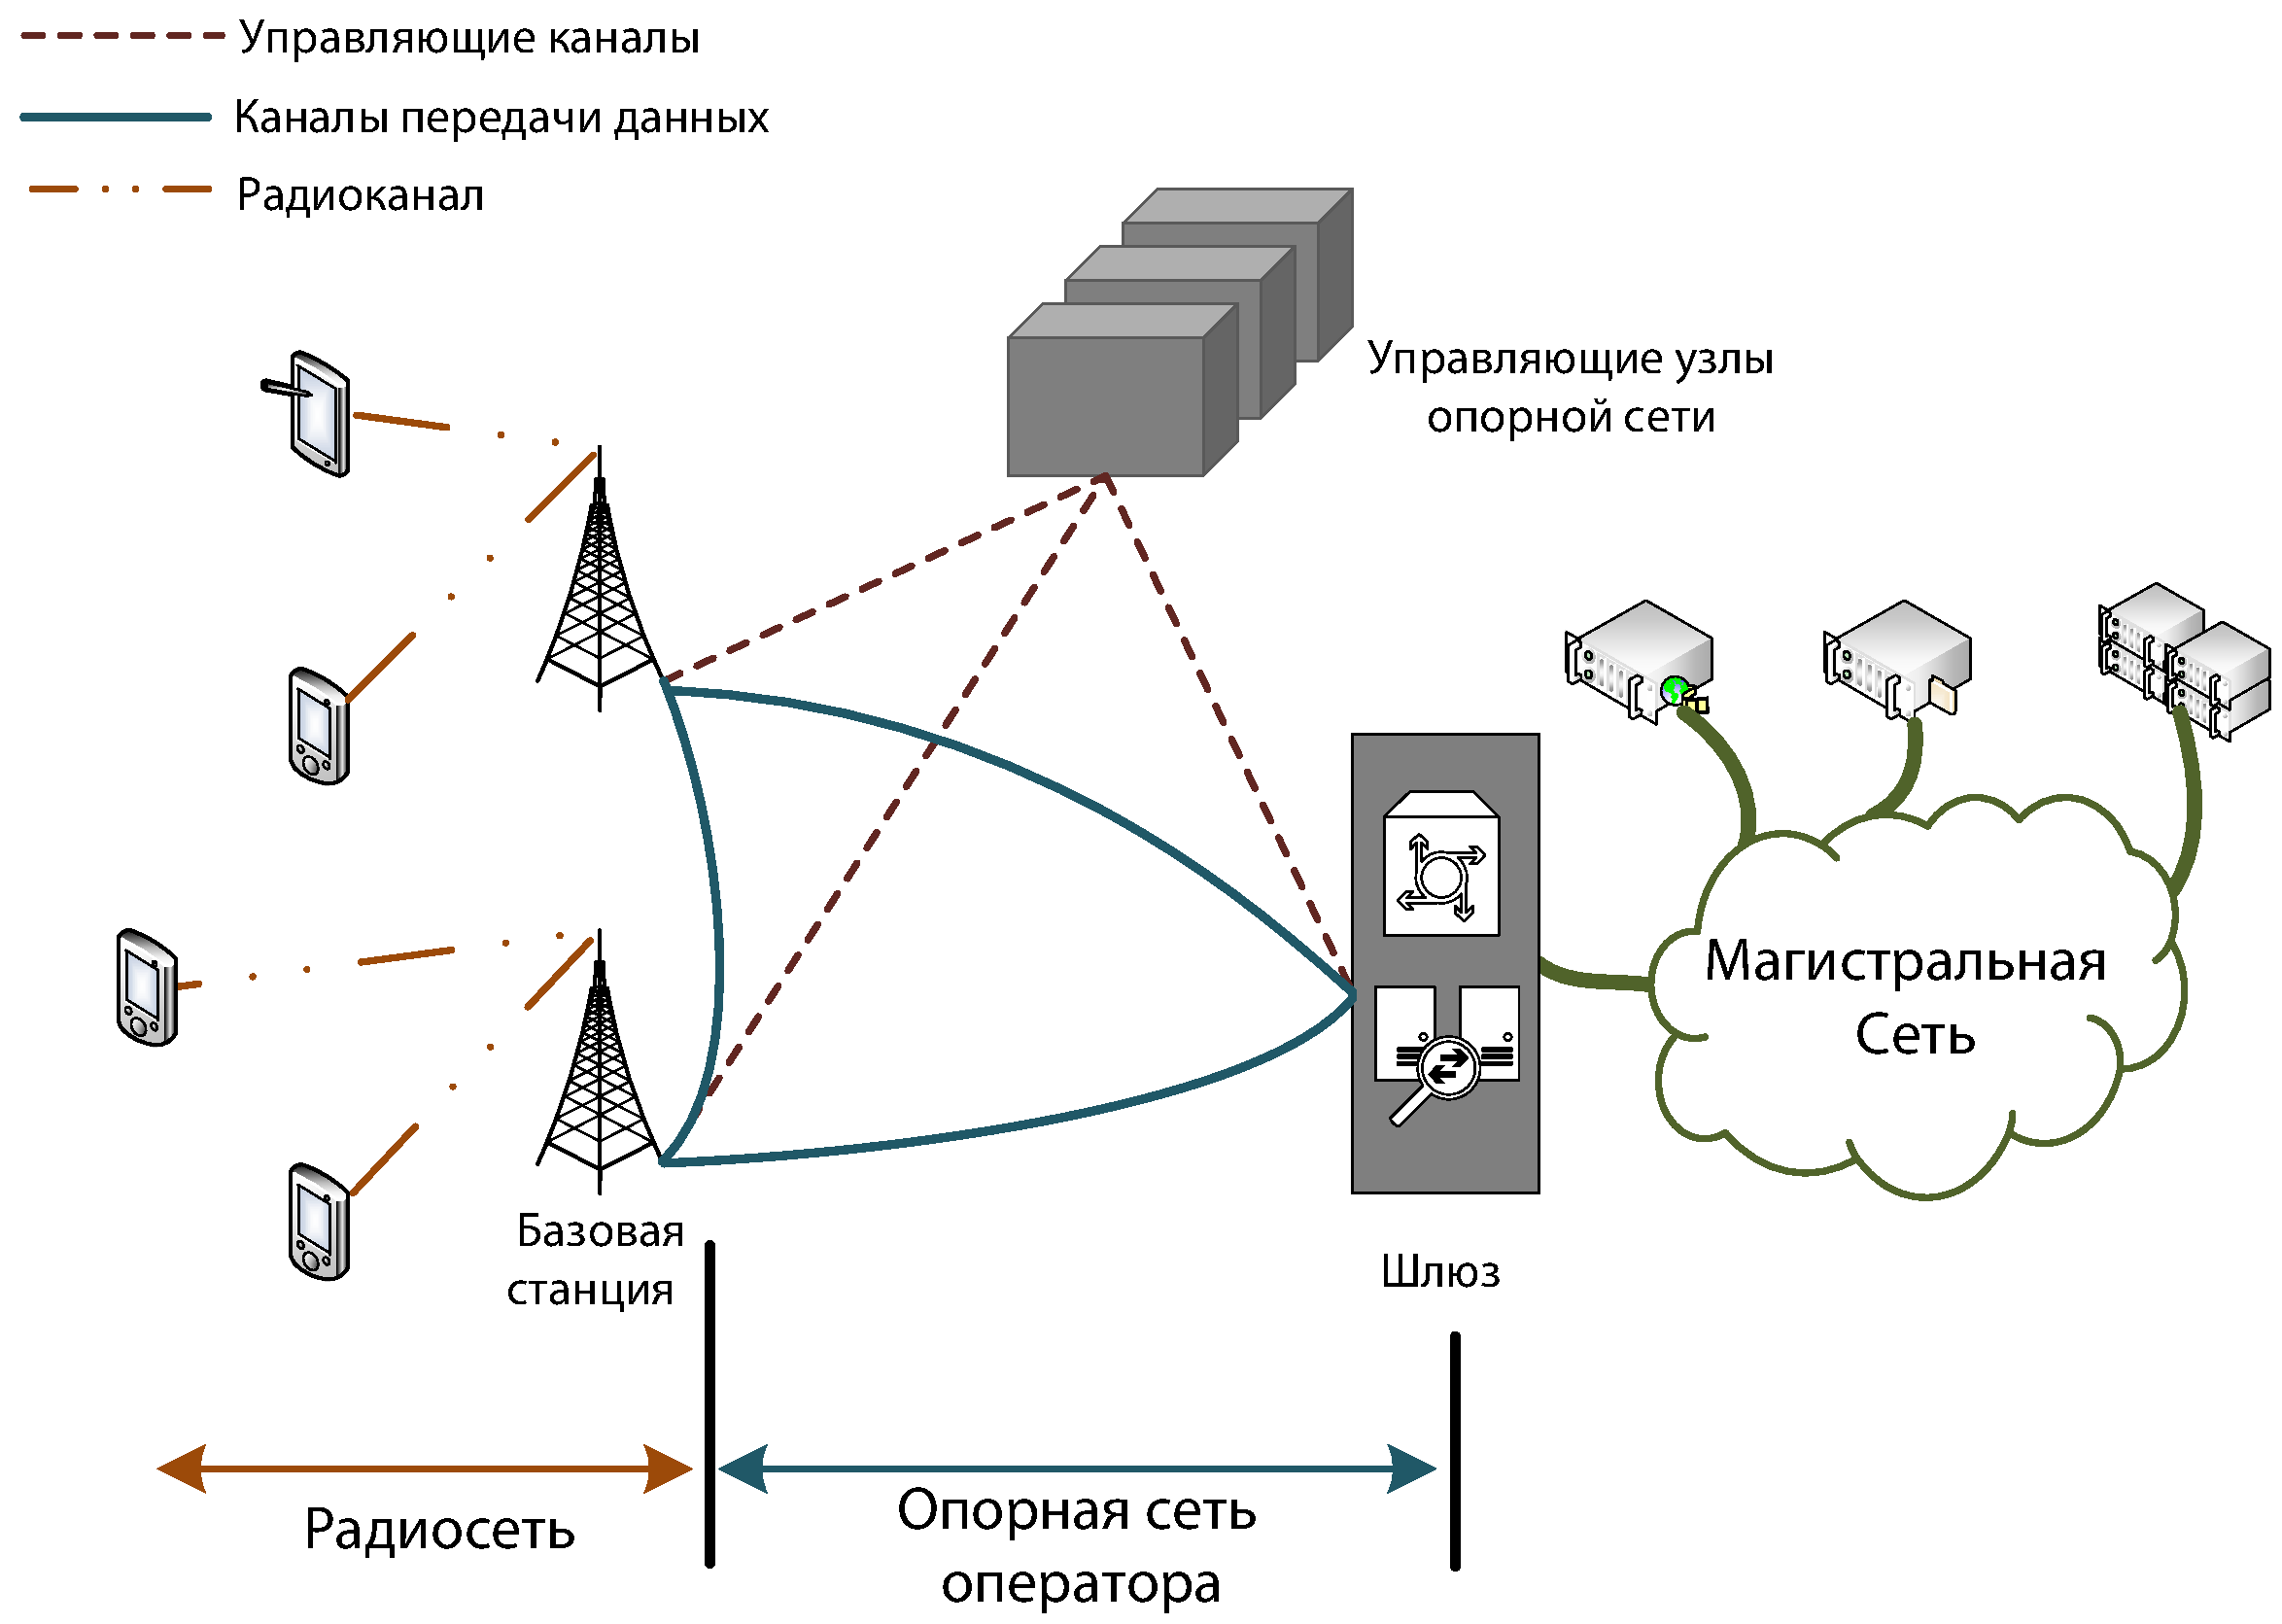
\includegraphics[width=\textwidth,height=0.4\textheight]{Chapter2/LteStucture.pdf}
\caption{Структура современных беспроводных централизованных систем}
\label{fig:LteStructure}
\end{center}
\end{figure}

Из представленной выше структуры, следует что аналитическая модель должна агрегировать в себе множество аспектов и параметров, присущих беспроводным централизованным системам, что делает ее сложной и многоуровневой. Как следствие, дальнейшее представление будет разделено на несколько этапов, последовательно описывающих представленную структуру:
\begin{itemize}
  \item Общие положения предлагаемой модели;
  \item Модель радиосети:
  \begin{itemize}
  	\item Модель беспроводного канала передачи данных;
  	\item Модель базовой станции.
  \end{itemize}
  \item Модель воспроизводящего устройства.
\end{itemize}
В завершении описания будет представлена система используемых допущений.

\section{Общие положения аналитической модели}
\label{chap2:GeneralOverview}

В настоящей работе рассматривается система с конечным числом абонентов: в системе находятся $N$ пользователей, которые используют сервис просмотра видеоконтента. Каждый пользователь обладает устройством с установленным видеоплеером и характеризуется уникальным номером~--~$i$, однозначно ассоциируемым с воспроизводящим устройством (на рисунках обозначается сокращенно <<Устр.~$i$>>).

В современных централизованных беспроводных системах базовые станции в различных сотах работают независимо друг от друга: невозможна ситуация, когда одно и тоже устройство обслуживают несколько станций одновременно. Решение о выделении ресурсов беспроводного канала на базовой станции принимается независимо, от работы базовых станций в соседних сотах. Следовательно, каждую соту возможно рассматривать как отдельную независимую систему, в которой необходимо производить оптимизацию передачи видео. На основании вышеизложенного, далее в работе будет рассматриваться работа только одной соты.

Все $N$ абонентов подключены по беспроводному каналу к одной базовой станции и имеют соединение с видеосервером, установленным в магистральной сети. Предполагается, что магистральные и опорные сети связи используют высокоскоростные каналы связи, что позволяет достигать колоссальных скоростей и минимально возможных задержек и джиттера при передаче данных. Таким образом, задержкой прохождение данных через данные участки сети можно пренебречь, и считать передачу данных через них мгновенной.

На удаленном видео сервере представлены видеоролики различной длительности в некотором наборе битовых репрезентаций (подраздел~\ref{chap1:VideoFormat}). Каждое видео представлено в виде последовательности из сегментов равной длительности $d$ секунд. Длительность видеопоследовательностей на видеосервере является некоторой случайной величиной $m$. Репрезентация каждой видеопоследовательности однозначно сопоставляется с битовой скоростью потока. Далее в работе, для обозначения битовой скорости потока сегмента $j$, просматриваемого пользователем $i$, будет использоваться нотация $R_{i,j}$. Предполагается, что все видеопоследовательности на видеосервере доступны в непрерывном отрезке битовых скоростей от $R_{min}$ до $R_{max}$:
\begin{equation}
R_{i,j} \in [R_{min}, R_{max}], i=\overline{1,N}.
\label{eq:BitrateConstr}
\end{equation}
В реальной системе непрерывность битовых скоростей может быть достигнута использованием на удаленном сервере транскодеров видеопотока. Транскодер~--~программный комплекс, позволяющий в режиме реального времени получать видеопоток с заданной битовой скоростью из потока с более высокой битовой скоростью. Использование траскодирования видеопотока позволяет видеоплееру подбирать битовую скорость видео под конкретные условия системы передачи видеоданных. Общая структура и особенности работы траскодеров видеопотока описаны в работах~\cite{1184336,1369700}.

Сегмент видеоданных $j$, при передаче через сеть пользователю $i$, представляется в виде последовательности из $P_{i,j}$ пакетов равного размера. Общий объем переданных данных в сегменте $j$ на пользовательское устройство $i$ составляет $R_{i,j} d$ бит.

Введем модель, описывающую поведение пользователя при просмотре видеоконтента. Каждый абонент просматривает серию видео (рисунок~\ref{fig:UeBehaviorModel}) путем отправки запросов на видеосервер и последовательной загрузки сегментов видеоданных через восходящий и нисходящий каналы связи соответственно. При заказе каждого сегмента видеоданных воспроизводящее устройство генерирует и отправляет на видеосервер уникальный запрос с указанием характеристик сегмента. В начале просмотра видео производится начальная буферизация, после окончания которой начинается демонстрация видеопотока и продолжится загрузка оставшихся видеоданных. После окончания просмотра видеопользователь $i$ через случайный интервал времени (паузу) $\tau_i$ закажет просмотр нового видео. Если скорости загрузки данных недостаточно для обеспечения просмотра видео, то могут возникнуть прерывания воспроизведения, вызванные необходимостью накопления достаточного объема видеоданных после опустошения буфера.

\begin{figure}[htbp]
\begin{center}
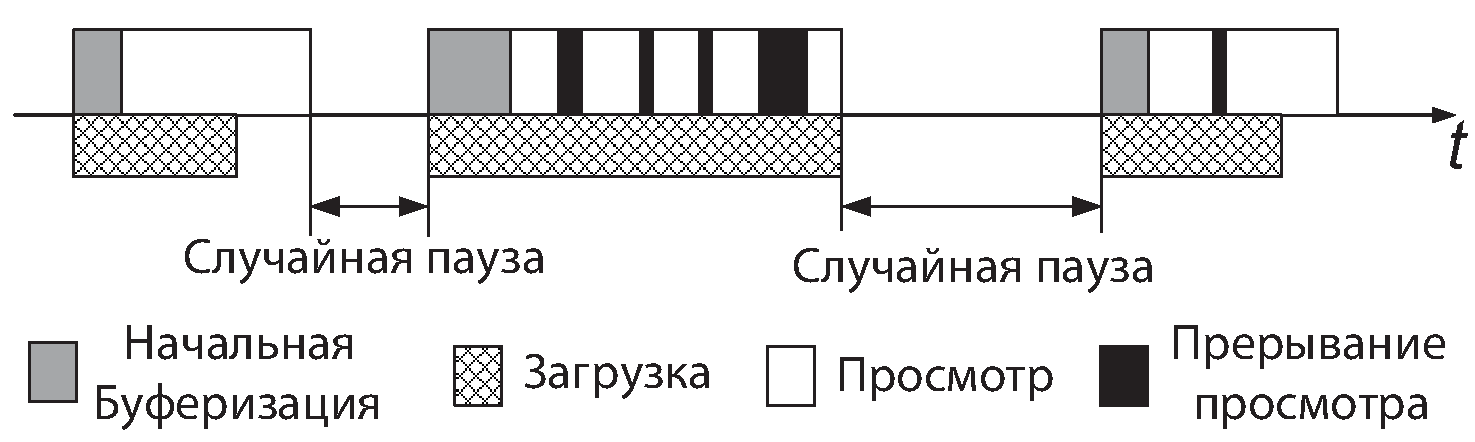
\includegraphics[width=\textwidth]{Chapter2/UeBehaviorModel.pdf}
\caption{Временная диаграмма поведения пользователя при просмотре видео}
\label{fig:UeBehaviorModel}
\end{center}
\end{figure}

Из модели поведения пользователя следует, что все время для конкретного пользователя можно разделить на три периода:
\begin{itemize}
	\item \textit{Буферизация}: пользователь ожидает начала или возобновления проигрывания видео (включает в себя начальные буферизации и прерывания воспроизведения, вызванные опустошением буфера);
	\item \textit{Просмотр}: штатное состояние, когда буфер на пользовательском устройстве достаточен и пользователь просматривает видеопоток;
	\item \textit{Пауза}: пользователь выбирает следующее видео для просмотра (в данном периоде просмотр и загрузка видео не осуществляются).
\end{itemize}
В дальнейшем будут использоваться обозначения $b_i^T$, $w_i^T$ и $p_i^T$ для обозначения общей длительности буферизации, просмотра и пауз пользователя $i$ за время в отрезке $[0, T]$ соответственно.

На уровне пользователя данную модель поведения возможно описать двумя основными характеристиками: коэффициентом разреженности видеопотока и отношением длительностей буферизации и просмотра для каждого конкретного пользователя.

\begin{definition}
\label{def:VideoSparseness}
    \emph{Коэффициент разреженности видеопотока пользователя $i$}~--~это отношение суммы длительностей просмотра и пауз к длительности просмотра пользователя $i$ за интервал времени $T\rightarrow\infty$:
    $$\gamma_i = \lim\limits_{T\rightarrow\infty} \frac{w_i^T + p_i^T}{w_i^T}.$$
\end{definition}

Коэффициент разреженности потока является величиной большей или равной единице: $\gamma_i \geq 1, i=\overline{1,N}$. Данное значение описывает активность пользователя при просмотре видео и показывает взаимосвязь между общим временем просмотра и пауз для конкретного абонента. Например, сравним двух пользователей $l$ и $r$, которые просмотрели одинаковую длительность видео за время $T$, однако $\gamma_l > \gamma_r$, это означает что пользователь $l$ делал большие паузы между просмотрами видео, чем пользователь $r$.

\begin{definition}
\label{def:BWTR}
    \emph{Отношение длительностей буферизации и просмотра}~--~это отношение общей длительности буферизации к длительности просмотра пользователя $i$ за интервал времени $T\rightarrow\infty$:
    $$q_i = \lim\limits_{T\rightarrow\infty} \frac{b_i^T}{w_i^T}.$$
\end{definition}

Отношение длительностей буферизации и просмотра для каждого пользователя является неотрицательной величиной: $q_i \geq 0, i=\overline{1,N}.$ Исходя из подраздела \ref{chap1:VideoMOS}, буферизация является негативным эффектом воспроизведения видео, который имеет критично большое влияние на качество восприятия абонентом сервиса передачи видеоданных. Как следствие, данный критерий обратно пропорционален удовлетворенности пользователя: чем больше значение $q_i$, тем меньше удовлетворенность пользователя.

\section{Модель беспроводного канала передачи данных}
\label{chap2:RadioChannel}

Одно из важнейших положений в описании представляемой аналитической модели занимает модель радиосети. В современных централизованных беспроводных системах радиосеть состоит из трех основных компонентов:
\begin{itemize}
	\item Беспроводной канал передачи данных;
	\item Базовая станция;
	\item Пользовательское устройство.
\end{itemize}

Опишем структуру и аспекты работы беспроводного канала. В существующих беспроводных централизованных сетях на физическом уровне ресурсы задаются двумя измерениями: частотой и временем (рисунок~\ref{fig:LteRadioChannel}). Во временной области все время работы разделено на периоды равной длительности, называемые слотами. Типовая длительность одного слота равняется 1-й миллисекунде (мс). В англоязычной литературе для обозначения слота используется Slot или Transmission Time Interval (TTI), обозначающие минимальное дробление времени для передачи данных. В частотной области вся полоса разделена на области равной ширины, в современных стандартах передачи данных ширина данных областей равняется 180 кГц. Минимальной единицей ресурсов является Ресурсный Блок~--~одна частотная область длительностью в один слот.

Множество ресурсных блоков формируют общий канал передачи данных, ресурсы которого могут быть распределены между пользователями в радиосети. Помимо общего канала связи реализованы служебные каналы, решающие задачи поддержания синхронизации и управления передачей пользовательских устройств, оценки качества канала, обеспечения надежной передачи данных по ненадежному каналу и т.д. Данные каналы занимают ресурсы в начале и внутри ресурсных блоков.

\begin{figure}[htbp]
\begin{center}
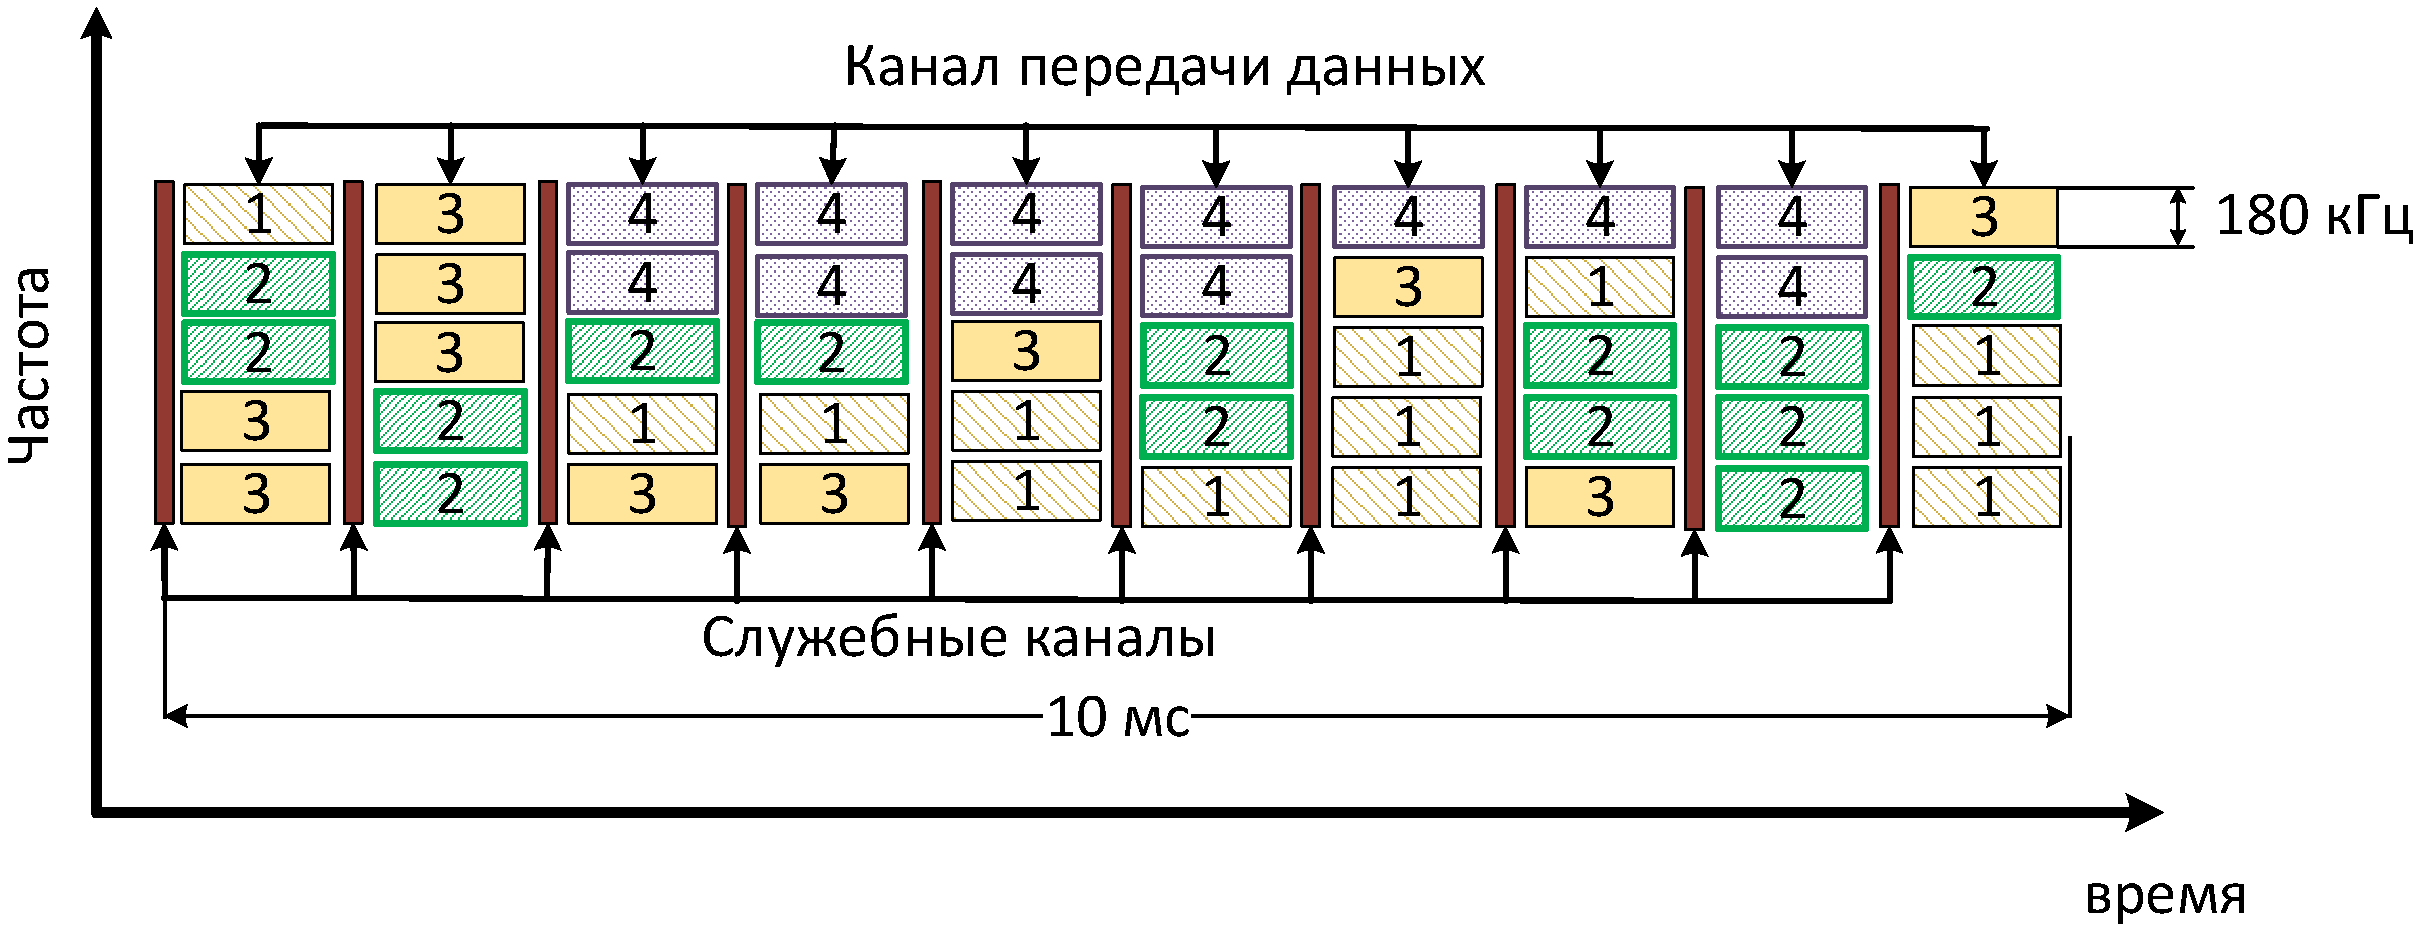
\includegraphics[width=\textwidth]{Chapter2/LteRadioChannel.pdf}
\caption{Структура беспроводного канала}
\label{fig:LteRadioChannel}
\end{center}
\end{figure}

Важной отличительной особенностью беспроводных каналов связи является изменчивость его характеристик как во времени, так и в частотной области. Подобная изменчивость вызвана наличием помех от работы других систем связи, движением пользователя и окружения, и т.д. Данный факт приводит к тому, что для одного абонента в разных ресурсных блоках может быть передан различный объем данных. Для каждого ресурсного блока на базовой станции вычисляется затухание распространения сигнала на основе информации от служебных каналов связи. Для описания качества канала на вышележащих уровнях базовой станции, полученное значение затухания сигнала для конкретного ресурсного блока и абонента преобразуется в кодо-модуляционную схему. Кодо-модуляционная схема (Modulation Code Scheme или MCS)~--~комбинация модуляции (QPSK, QAM-16, QAM-64) и настроек помехоустойчивого кодирования. %Значение кодо-модуляционной схемы имеет прямую корреляцию с уровнем качества канала: чем выше значение MCS, тем выше качество канала. Используемая кодо-модуляционная схема определяет количество байт, которое возможно передать в конкретном ресурсном блоке.

Рассматриваемая модель предполагает, что пользователи в соте могут находится в различных условиях беспроводного канала, вызванные удаленностью от базовой станции и движением абонента и окружения. Последовательно рассмотрим восходящий и нисходящий беспроводные каналы. В современных централизованных системах связи восходящий канал обладает сравнимыми характеристиками с нисходящим, однако, его загруженность несравнимо меньше по сравнению с нисходящей линией связи. Как следствие, восходящий канал связи считается абсолютно надежным и задержкой передачи запросов на сегменты видео можно пренебречь.

Аналитическая модель уделяет большое внимание нисходящему каналу связи, так как от его производительности зависит удовлетворенность пользователей в соте. В данной работе рассматривается модель канала, обладающая следующим свойством: затухание при распространении сигнала происходит одинаково по всей ширине полосы передачи данных для конкретного пользователя в одном моменте времени. В реальной системе данное допущение приводит к равенству значений выбранных кодо-модуляционных схем для всех ресурсных блоков в рамках одного слота конкретного пользователя. Следствием равенства кодо-модуляционных является равенство возможного передаваемого объема данных для всех ресурсных блоков в слоте.

Таким образом, состояние беспроводного канала пользователя $i$ возможно охарактеризовать максимально достижимой скоростью канала.
\begin{definition}
\label{def:MaxThroughput}
    \emph{Максимально достижимая скорость канала пользователя $i$}~--~скорость передачи данных по беспроводному каналу, если все доступные ресурсы были выделены $i$-му пользователю.
\end{definition}
Данная величина является аналогичной скорости передачи данных, при условии, что пользователь $i$ находится один в соте. Далее в работе, для обозначения максимально достижимой скорости канала пользователя $i$ будет использоваться обозначение $C_i$, а для сокращения текста слово <<максимальная>> будет опускаться.

Для каждого пользователя $i$ существует случайный процесс изменения затухания при распространении сигнала и замираний от времени $L_i(t)$. На основе значения $L_i(t)$ в момент времени $t$ на базовой станции подбирается кодо-модуляционная схема, таким образом, что вероятность ошибки при передаче данных является пренебрежимо малой величиной. Выбранная кодо-модуляционная схема определяет максимальную пропускную канала $C_i(t)$ в момент времени $t$.

Предполагается, что состояние беспроводного канала изменяется, таким образом, что в течении загрузки пакета $k$ из сегмента $j$ максимально достижимая скорость канала пользователя $i$ постоянна:
\begin{equation}
C_i(t)=C_{i,j,k}, t_{i,j,k} \leq t \leq t_{i,j,k}+\Delta t_{i,j,k},
\label{eq:ChannelConst}
\end{equation}
где $t_{i,j,k}$~--~момент времени начала загрузки пользователем $i$ пакета $k$ из сегмента $j$, $\Delta t_{i,j,k}$~--~длительность загрузки пользователем $i$ пакета $k$ из сегмента $j$, $C_{i,j,k}$~--~максимально достижимая скорость канала пользователя $i$ в течении загрузки пакета $k$ из сегмента $j$.

%Для современных централизованных беспроводных сетей в типовой соте для передачи информации в одном слоте доступны 48 ресурсных блоков (ширина полосы 10 МГц), и при использовании кодо-модуляционной схемы с модуляцией QPSK в одном слоте возможно передать 900 байт полезной информации. Таким образом, для пользователя в плохих радиоусловиях пакет может быть передан за 2 миллисекунды (подраздел~\ref{chap1:VideoFormat}). Данный факт демонстрирует, что представленное ограничение не сужает возможную сферу применения предлагаемой модели беспроводного канала.

Введем дополнительное обозначение $C_{i,j}^{-1}$ равное выборочному среднему для величин обратных к максимально достижимой скорости при передачи пакетов в течение одного сегмента видеоданных:
\begin{equation}
\nonumber
C_{i,j}^{-1} = \frac{1}{P_{i,j}}\sum\limits_{k=1}^{P_{i,j}} \frac{1}{C_{i,j,k}},
\label{eq:ChannelConst_v1}
\end{equation}
где $P_{i,j}$~--~число пакетов в сегменте $j$ пользователя $i$.

\section{Распределение ресурсов беспроводного канала связи}
\label{chap2:Scheduler}

После определения структуры беспроводного канала необходимо привести описание того как, используя данную структуру, происходит обмен данными между базовой станций и пользовательским устройством. Для этого рассмотрим функциональную структуру базовой станции.

Основной задачей базовой станции, является организация надежной передачи данных по ненадежному радиоканалу. Для решения данной задачи используется структура, состоящая из четырех уровней (рисунок~\ref{fig:eNbLayers}):
\begin{itemize}
	\item Уровень обработки пакетов;
	\item Уровень очередей для передачи данных по беспроводному каналу связи;
	\item Уровень доступа ко среде передачи данных;
	\item Уровень физической среды.
\end{itemize}

\begin{figure}[htbp]
\begin{center}
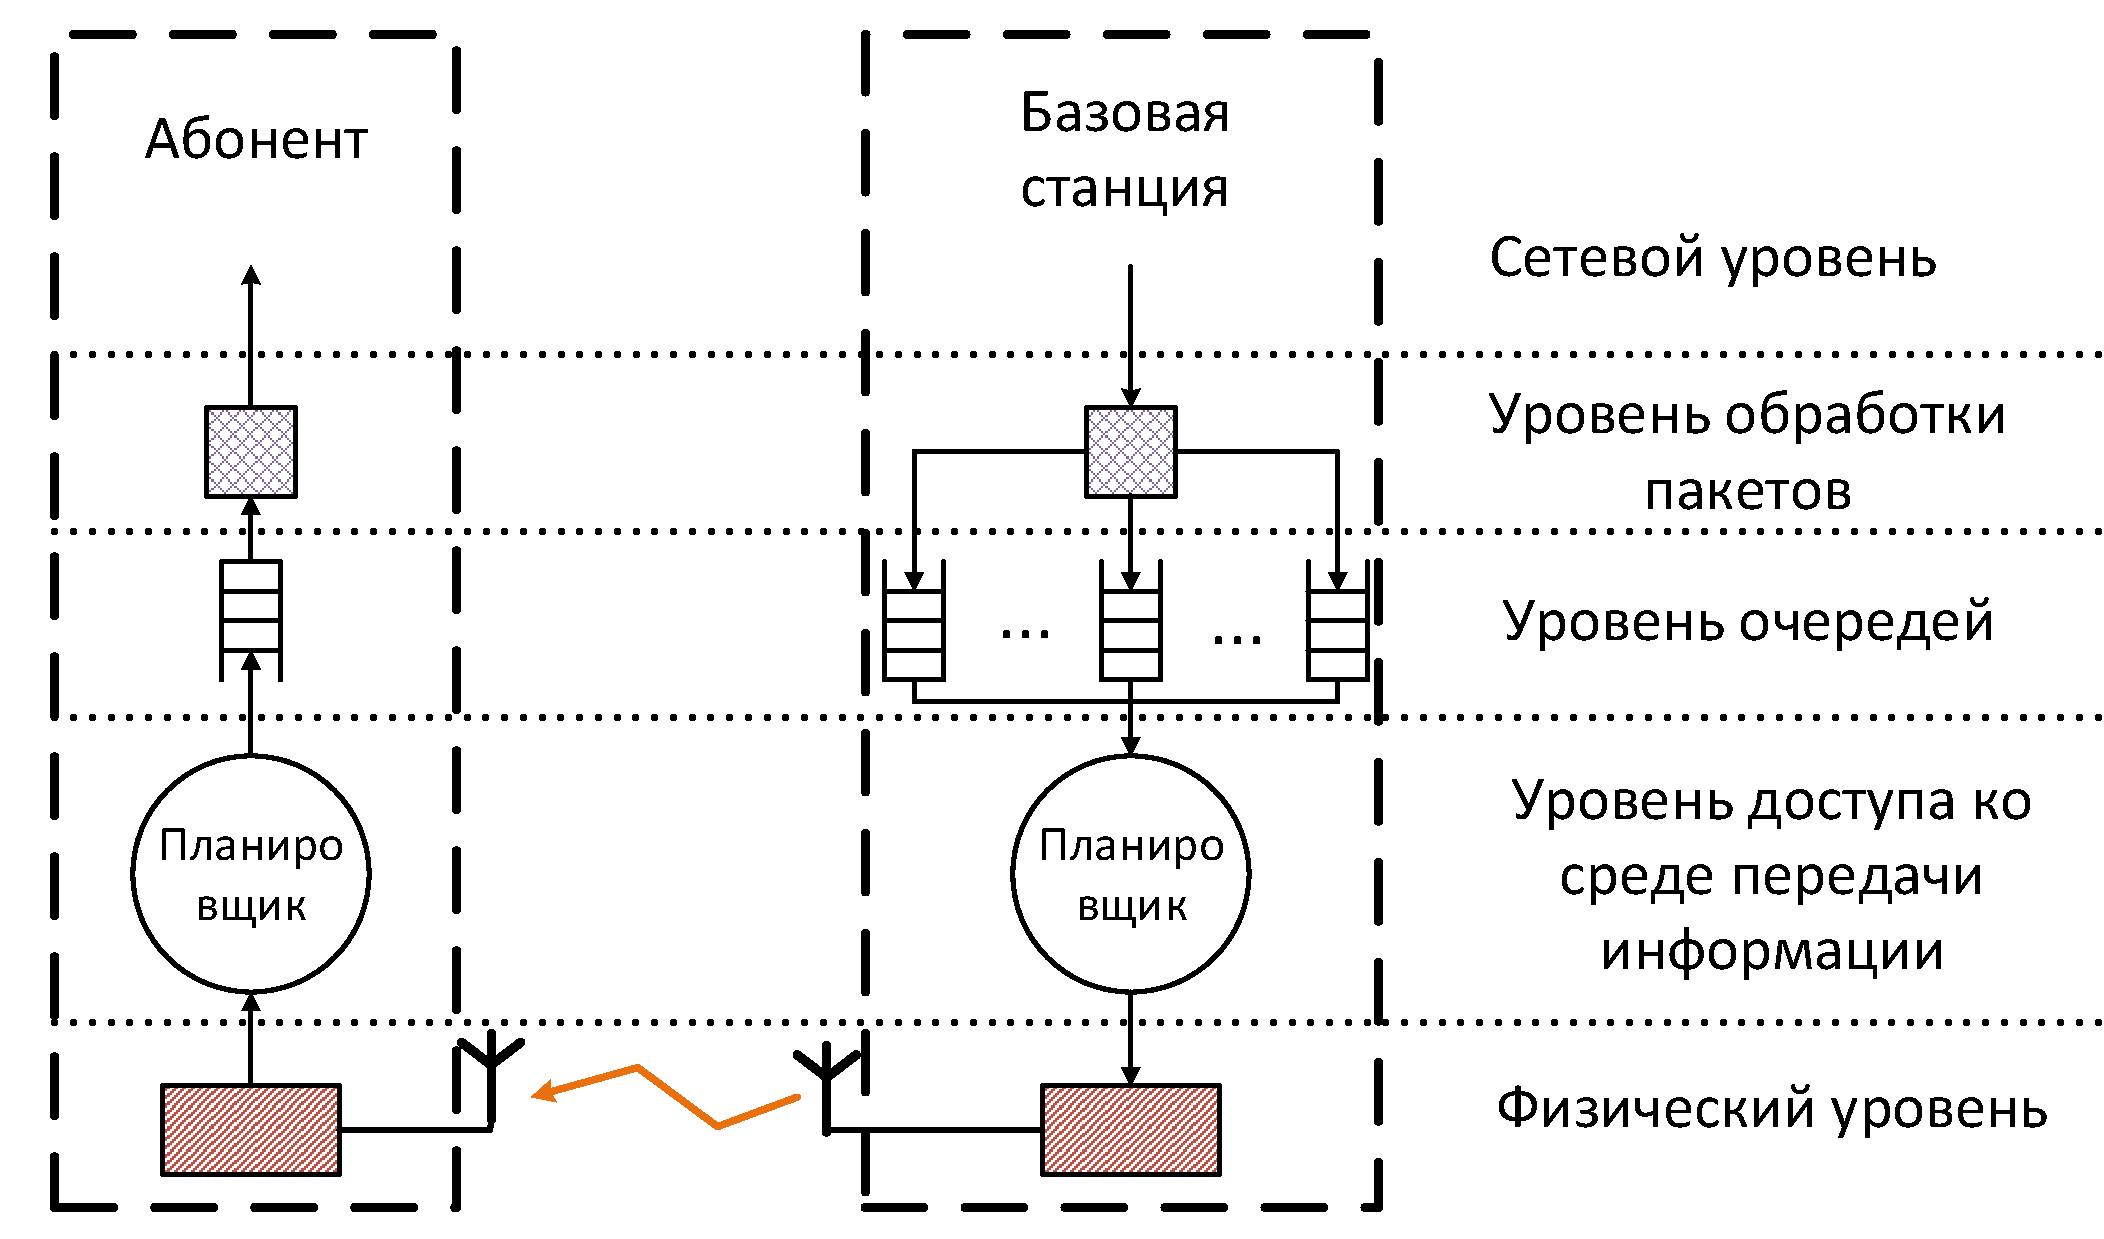
\includegraphics[width=\textwidth,height=0.4\textheight]{Chapter2/eNbLayers.pdf}
\caption{Функциональная структура базовой станции и пользовательского устройства}
\label{fig:eNbLayers}
\end{center}
\end{figure}

Опишем доставку пакета с данными от момента его получения на базовой станции, до момента его появления на сетевом уровне пользовательского устройства. Из опорной сети оператора пакет попадает на уровень обработки пакетов, данный уровень выполняет две функции. Первой функцией является сжатие заголовков пакетов транспортного и сетевого уровня, для уменьшения объема передаваемых данных по беспроводному каналу. Реализация сжатия заголовков пакета позволяет нивелировать накладные издержки при передаче данных по беспроводному каналу и считать, что в пакете нет никакой избыточности, добавляемой сетевыми протоколами. Второй функцией является определение абонента и передача информационной части пакета в его очередь на нижележащем уровне.

Ниже расположен уровень очередей для передачи данных по беспроводному каналу связи. На данном уровне для каждого пользователя, подключенного к базовой станции, расположена очередь (буфер) для данных. Уровень очередей является промежуточным между уровнями обработки пакетов и канального уровня, выполняющего роль временного хранилища данных при их передаче по беспроводному каналу. Обслуживанием очередей занимается нижележащий уровень: уровень доступа ко среде передачи (Medium Access Control или MAC).

Уровень доступа ко среде передачи данных решает ключевую задачу для системы в целом: на основе информации от уровня физической среды и вышележащих уровней базовой станции произвести распределение ресурсов беспроводного канала и обеспечить надежность передачи данных. Решением данной задачи занимается планировщик ресурсов беспроводного канала, установленный на базовой станции (в англоязычной литературе используется обозначение Media Access Channel Scheduler или MAC Scheduler). Далее в работе для сокращения объема текста в качестве обозначения <<планировщика ресурсов беспроводного канала>> будет использоваться термин <<планировщик>>.

Планировщик в каждом слоте производит распределение ресурсов радиоканала (ресурсных блоков) в соответствие с некоторым алгоритмом. Важно отметить, что планировщик не выделяет ресурсы абонентам, у которых нет данных в данном слоте. В каждом слоте формируется карта распределения ресурсных блоков, которая будет передана на физический уровень. На рисунке~\ref{fig:LteRadioChannel} представлен пример распределения ресурсов в течении десяти слотов для четырех активных пользователей. Таким образом, работу алгоритма планирования можно представить в виде распределения долей канала между пользователями. Например, в первом слоте пользователям $1$, $2$ и $3$ были выделены доли беспроводного канала $0.2$, $0.4$ и $0.4$ соответственно.

Сформированная карта распределение ресурсных блоков будет передана на уровень физической среды, который обеспечит передачу данных из уровня очередей в выделенных частотно-временных ресурсах. В дальнейшем, при корректной работе всех описанных уровней базовой станции пакет будет доставлен по беспроводному каналу на пользовательское устройство и, пройдя стек в обратном порядке, станет доступен на сетевом уровне пользовательского устройства.

Несмотря на важную роль планировщика, алгоритмы планирования не стандартизованы для существующих систем связи, поэтому каждый производитель базовых станций использует собственные реализации алгоритмов планирования. Создание подобных алгоритмов является открытой задачей, так как требования к ним очень обширны и не существует строгих теоретических исследований о их максимальной производительности. В настоящее время известны два эвристических алгоритма планирования ресурсов: Proportional Fair \cite{1310314} и Round Robin \cite{miao_zander_sung_ben_slimane_2016}. Алгоритм планирования Proportional Fair ставит своей задачей обеспечения равных скоростей передачи данных для всех активных пользователей. Алгоритм планирования Round Robin обеспечивает равный доступ к ресурсам радиоканала для всех активных пользователей. Поэтому настоящая диссертационная работа ставит своей основной задачей исследование алгоритмов планирования, с целью увеличения их производительности и, как следствие, всей беспроводной централизованной сети для передачи видеоданных.

Центральное положение, в представляемой аналитической модели, занимает алгоритм планирования распределения ресурсов беспроводного канала, установленный на базовой станции. Введем определение алгоритма планирования:

\begin{definition}
\label{def:SchedulingAlg}
    \emph{Алгоритм планирования}~--~это правило, в соответствии с которым базовая станция в момент времени $t$ распределяет доли ресурсов беспроводного канала $\alpha_i(t) \geq 0$ для пользователя $i$.
\end{definition}

Таким образом, работу алгоритма планирования в момент времени $t$ возможно описать вектором значений функций: ${A}(t) = \left\{\alpha_{i}(t), i = \overline{1,N}\right\}$. Очевидным ограничением на возможные значения функций $\alpha_i(t)$ является следующее неравенство:
\begin{equation}
\forall t: \sum\limits_{i=1}^{N}\alpha_{i}(t) \leq 1.
\label{eq:sumAlpha}
\end{equation}
Неравенство (\ref{eq:sumAlpha}) может быть интерпретировано следующим образом: в любой момент времени работы алгоритма планирования общий объем выделенных ресурсов не превышает доступного объема ресурсов для канала передачи данных. Следовательно, для любого пользователя $i$, мгновенная скорость передачи данных в нисходящем канале связи $S_i(t)$ может быть вычислена следующим образом:
\begin{equation}
S_i(t) = \alpha_i(t) C_i(t).
\label{eq:MomentRate}
\end{equation}

Алгоритм планирования в каждый момент времени решает задачу распределения ресурсов беспроводного канала. Для решения данной задачи ему доступна информация о предыстории, а именно доли выделенных ресурсов канала, значения максимально достижимых скоростей канала и объем переданных данных для каждого пользователя:
\begin{equation}
A(t) = \mathcal{A}\left( S_i(\tau), C_i(\tau);\tau<t, i=\overline{1,N} \right),
\label{eq:SchedulingRule}
\end{equation}
где $\mathcal{A}\left(\cdot\right)$ является алгоритмом планирования. В формуле (\ref{eq:SchedulingRule}) информация о предыстории выделенных долей беспроводного канала и объемах переданных данных для пользователя $i$ агрегированы в значении $S_i(\tau)$, так как данные параметры задаются соотношением (\ref{eq:MomentRate}).

Важно отметить факт, что для планировщика базовой станции пользователь в каждый момент времени может находиться в одном из двух состояний: активном и неактивном. Пользователь считается активным, если у данного пользователя есть данные для передачи в нисходящем канале на базовой станции, иначе пользователь считается неактивным. В реальной системе, активность абонента так же определяется на основе наполненности очередей. Основываясь на модели поведения пользователя при просмотре видео, пользователь может является активным только в период осуществления загрузки данных (рисунок~\ref{fig:UeBehaviorModel}). Важно отметить, что загрузка данных состоит из последовательной передачи пакетов с видеоданными, и пользователь считается неактивным во время пауз между их загрузками.

В данной диссертационной работе рассматриваются алгоритмы планирования, которые удовлетворяют представленному ниже набору свойств:
\begin{itemize}
	\item В каждый момент времени активному пользователю гарантировано выделение минимальной доли ресурсов канала $\alpha_{i}^{min}$:
	\begin{equation}
		\label{eq:MinGuarPart}
		\begin{cases}
			\alpha_i(t) = 0, & \text{пользователь $i$ неактивен в момент времени $t$} \\
			\alpha_i(t) \geq \alpha_{i}^{min}, & \text{пользователь $i$ активен в момент времени $t$}\\
		\end{cases}.
	\end{equation}
	Минимальная доля ресурсов канала является величиной, отличной от нуля: $\alpha_{i}^{min} > 0$, и сумма минимальных долей ресурсов канала для всех пользователей не превышает общего объема ресурсов, доступных для планирования: $\sum\limits_{i=1}^{N}\alpha_{i}^{min} \leq 1$.
	\item Ресурсы беспроводного канала не могут быть выделены неактивному абоненту.
	\item В каждый момент времени планировщик распределяет все доступные ресурсы между активными абонентами:
\end{itemize}
\begin{equation}
	\label{eq:AllResources}
	\sum\limits_{i=1}^{N}\alpha_{i}(t) =
	\begin{cases}
		0, & \text{в момент времени $t$ все пользователи неактивны} \\
		1, & \text{иначе}\\
	\end{cases}.
\end{equation}

\section{Модель воспроизводящего устройства}
\label{chap2:VideoTrafficModel}

В завершении представлении аналитической модели будет определена модель видеотрафика и видиоплеера. В данной работе предполагается, что видеоплеер и видеосервер поддерживают технологию адаптивной передачи видеоконтента DASH (подраздел~\ref{chap1:VideoPlayers}) (рисунок~\ref{fig:PlayerModel}). Видеоплеер, установленный на пользовательском устройстве, осуществляет последовательную загрузку сегментов видеопоследовательности: следующий сегмент видео может быть заказан после окончания загрузки предыдущего и некоторой задержки. Пауза между заказами обусловлены стратегией наполнения буфера и моделью поведения пользователя. Данная задержка может быть короткой, если загружается сегмент в середине видео и достаточной длинной, если загружается первый сегмент, в случае если данная задержка включает в себя случайную паузы между просмотрами видеопоследовательностей, представленные на рисунке~\ref{fig:UeBehaviorModel}.

\begin{figure}[htbp]
\begin{center}
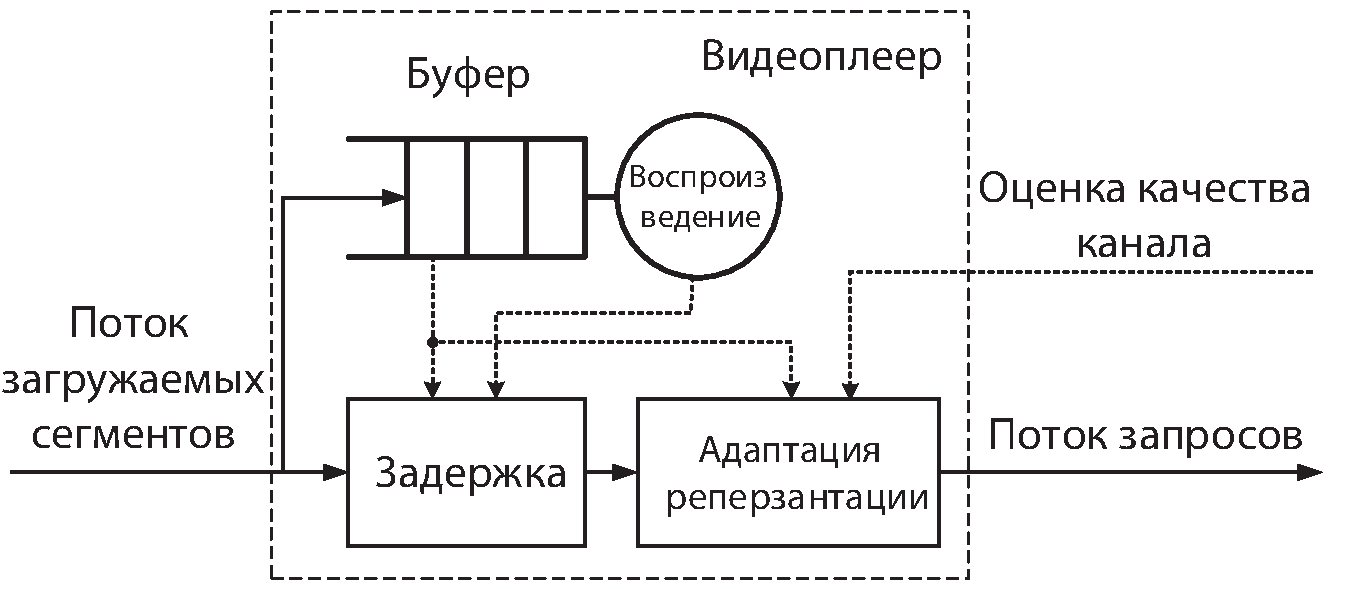
\includegraphics[width=0.8\textwidth]{Chapter2/PlayerModel.pdf}
\caption{Модель воспроизводящего устройства}
\label{fig:PlayerModel}
\end{center}
\end{figure}

При заказе нового сегмента видеопоследовательности видеоплеер решает задачу выбора репрезентации для заказываемого сегмента. В предлагаемой модели репрезентация сегмента однозначно сопоставлена с битовой скоростью, таким образом задача выбора репрезентации сводится к задаче адаптации битовой скорости потока. Для решения данной задачи видеоплеер может использовать информацию о наполненности буфера и других статистиках: оценку скорости получения данных в течении предыдущих сегментов, информацию о качестве беспроводного канала и т.д. Задача адаптации битовой скорости потока может быть представлена следующим выражением:
\begin{equation}
\nonumber
R_{i,j} = \mathcal{B}\left(R_{i,k}, C_i(\tau), S_i(\tau); k < j, \tau<t_{i,j} \right),
\end{equation}
где $\mathcal{B}\left(\cdot\right)$ является функцией вычисления битовой скорости $j$-го сегмента пользователя $i$, $R_{i,j}$~--~битовая скорость потока $j$-го сегмента пользователя $i$.

Из описания, представленного в подразделе \ref{chap1:VideoPlayers}, следует, что часто на функцию $\mathcal{B}\left(\cdot\right)$ наложено ограничение на число переключений репрезентаций в единицу времени. Обычно адаптация видеопотока под конкретные условия беспроводного канала происходит в короткий промежуток времени в начале загрузки нового видео. Таким образом, если существуют математическое ожидание: $E[R_i] = \lim\limits_{j \rightarrow \infty}E[R_{i,j}]$ и среднее квадратичное отклонение: $\sigma\left[R_{i}\right] = \lim\limits_{j \rightarrow \infty}\sigma\left[R_{i,j}\right] $ битовой скорости просматриваемого потока, то коэффициент вариации битовой скорости видеопотока ограничен сверху некоторой постоянной, значение которой зависит от типа и настроек видеоплеера:
\begin{equation}
\forall i: \frac{ \sigma\left[R_{i}\right] }{ E\left[R_{i}\right]} \leq \nu^R_i.
\label{eq:SwitchRatio}
\end{equation}

Введение модели видеоплеера завершает описание аналитической модели. Обобщая описанное выше, предлагается следующая система допущений для аналитической модели передачи видеоданных в централизованных беспроводных сетях.

\section{Система допущений для модели передачи видеоданных}
\label{chap2:Assumptions}

Общая структура предложенной аналитической модели передачи видеоданных представлена на рисунке~\ref{fig:SystemModel}. В представленной структуре магистральная и опорная сети были объедены в магистральную сеть передачи данных, ввиду схожести их характеристик. Ниже представлен список используемых допущений в настоящей работе.

\begin{figure}[htbp]
\begin{center}
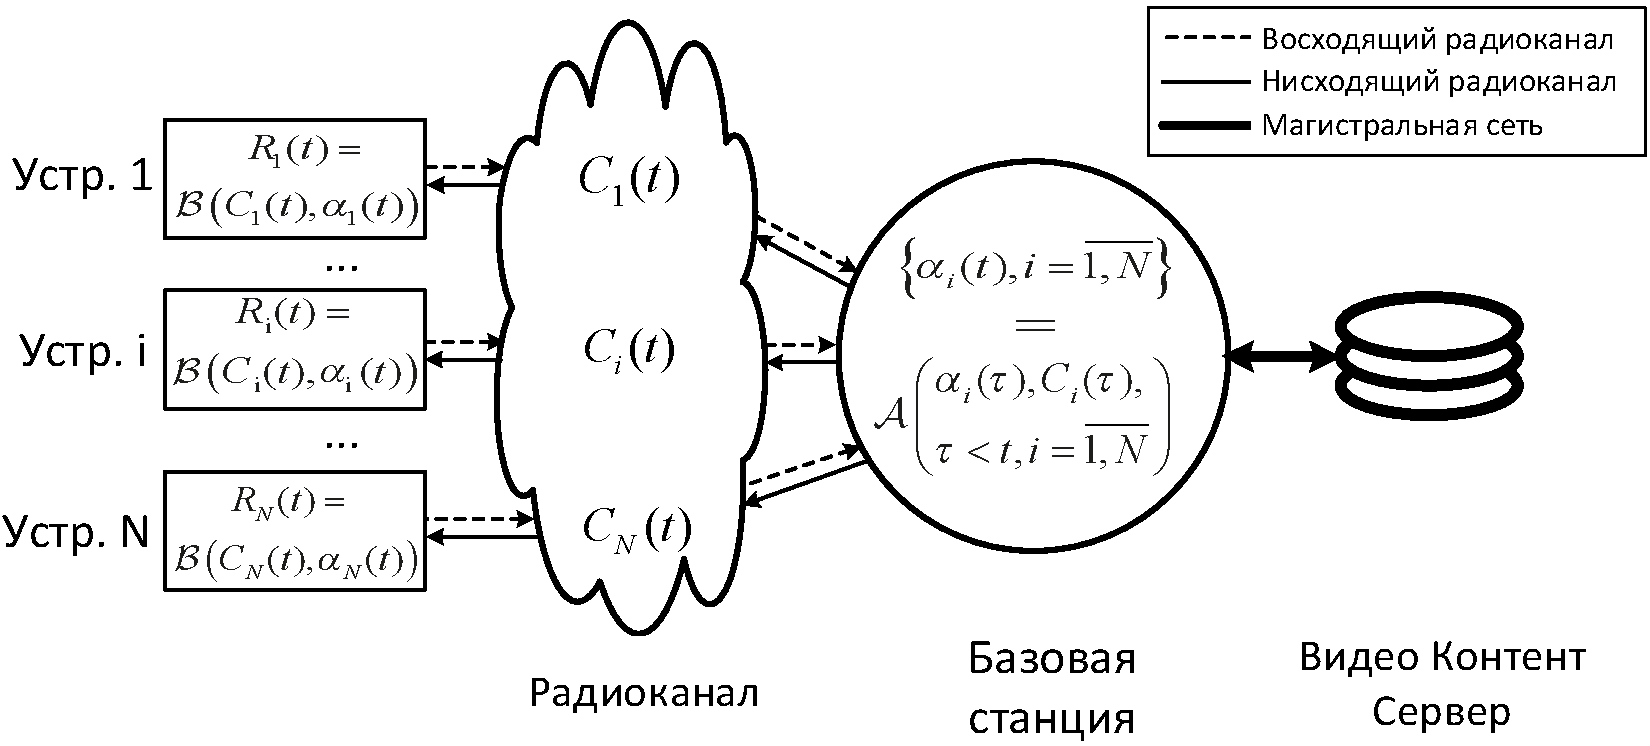
\includegraphics[width=\textwidth]{Chapter2/SystemModelEch.pdf}
\caption{Структура модели передачи видеоданных в централизованных беспроводных сетях}
\label{fig:SystemModel}
\end{center}
\end{figure}

\begin{itemize}
	\item \textit{Формат представления видеоданных}:
		\begin{enumerate}
			\item Все видеопоследовательности разбиты на сегменты одинаковой длительности $d$ секунд;
			\item Каждый сегмент видеоданных $j$ пользователя $i$ представляется в виде последовательности из $P_{i,j}$ пакетов равного объема;
			\item Все видеопоследовательности на Видеосервере представлены в непрерывном отрезке битовых скоростей (\ref{eq:BitrateConstr});
			\item Длительность видеопоследовательностей, представленных на видео сервере, является независимой случайной величиной с конечным математическим ожиданием и дисперсией.
		\end{enumerate}
	\item \textit{Общие характеристики сети передачи данных}:
		\begin{enumerate}
			\item Задержка в восходящем канале считается пренебрежимо малой;
			\item Загрузка сегментов видеоданных начинается незамедлительно в момент отправки запроса.
		\end{enumerate}
	\item \textit{Модель поведения пользователя при просмотре видео}:
		\begin{enumerate}
			\item Паузы между просмотрами $\tau_i$ является независимыми случайными величинами с конечными математическим ожиданием ($\overline{\tau}_i$) и дисперсией.
		\end{enumerate}
	\item \textit{Модель беспроводного канала}:
		\begin{enumerate}
			\item Затухание сигнала при распространении происходит одинаково по всей ширине полосы передачи данных для конкретного пользователя в одном моменте времени;
			\item Кодо-модуляционная схема подбирается таким образом, что вероятность ошибки при передаче данных по беспроводному каналу пренебрежимо мала;
			\item В течении передачи одного пакета $k$ из сегмента $j$ пользователем $i$ в нисходящей линии связи максимально достижимая скорость канала постоянна (\ref{eq:ChannelConst});
			\item Последовательности случайных величин $C^{-1}_{i,1}, C^{-1}_{i,2}, \ldots, i=\overline{1,N}$ формируют эргодические случайные процессы с конечными математическими ожиданиями $E[C_i^{-1}]$ и коэффициентами вариации $\nu^{C}_i$ соответственно.
		\end{enumerate}
	\item \textit{Модель планировщика ресурсов беспроводного канала}:
		\begin{enumerate}
			\item Алгоритм планирования выделяет частотно-временные ресурсы только активным абонентам;
			\item Алгоритм планирования гарантирует каждому активному абоненту минимальную долю ресурсов беспроводного канала в каждом интервале планирования (\ref{eq:MinGuarPart});
			\item Алгоритм планирования распределяет все доступные частотно-временные ресурсы (\ref{eq:AllResources}).
		\end{enumerate}
	\item \textit{Модель видеоплеера}:
		\begin{enumerate}
			\item Последовательности $R_{i,1}, R_{i,2}, \ldots, i=\overline{1,N}$ формируют эргодические случайные процессы с конечными математическими ожиданиями $E[R_{i}]$ и коэффициентами вариации не превышающими значений $\nu^R_i$ (\ref{eq:SwitchRatio}) соответственно.
		\end{enumerate}
  \item \textit{Дополнительные обозначения}:
  \begin{enumerate}
  \item $\mathcal{A}$~--~множество алгоритмов планирования на базовой станции, удовлетворяющих введенным допущениям;
  \item $\mathcal{B}$~--~множество алгоритмов адаптации репрезентации на пользовательских устройствах, удовлетворяющих введенным допущениям.
  \end{enumerate}
\end{itemize}
Система допущений завершает представление аналитической модели.

\section{Система передачи видеоданных как система массового обслуживания}
\label{chap2:QueuningNetwork}

Представленная выше аналитическая модель передачи видеоданных описывает достаточно современные тенденции развития телекоммуникационных сетей связи: передача видео и беспроводные сети. Аналогичные системы рассматривались еще в 70-х годах 20-го века, они известны как замкнутые системы массового обслуживания (СМО) с конечным числом абонентов. Далее предлагается краткое описание таких СМО и анализ отличий данных систем от рассматриваемой модели в настоящей работе.

Изначально, СМО с конечным числом абонентов были рассмотрены Шерром в работе \cite{scherr}, в дальнейшем замкнутые СМО с конечным числом абонентов были широко исследованы в работах \cite{adiri, simha, veran}. Общая идеология таких систем состоит в следующем. Абонент отправляет на обслуживающий прибор заявку, которая становится в очередь бесконечного размера. Заявки всех абонентов считаются одинаковыми. Обслуживающий прибор, исходя из зафиксированной дисциплины обслуживания, обрабатывает заявки в очереди. Когда заявка для некоторого абонента была обслужена, то по петле обратной связи для этого абонента будет доставлено уведомление об окончании выполнения заявки. После получения уведомления абонент отправляет следущую заявку в систему через некоторую паузу. В классических СМО с конечным числом абонентов время между получением уведомления об обработки заявки до посылки нового запроса в систему и длительность обслуживания заявки в очереди распределено по экспоненциальному закону.

Важной особенностью подобных систем является то, что в каждый момент времени в очереди на обслуживающем приборе количество заявок не превосходит количество абонентов в сети. Данный факт приводит к тому, что среднее время обслуживания абонентов до точки насыщения системы растет незначительно, а после нее растет линейно, с углом наклона зависящего от интенсивности обслуживания и временем между получением уведомления и отправки новой заявки. Такое поведение среднего времени обслуживания отличается от классических СМО без обратной связи, в которых оно растет экспоненциально после достижения системой точки насыщения, в виду бесконечного роста количества заявок в очереди на обслуживающем приборе.

Опишем систему передачи видеоданных в терминах замкнутых СМО с конечным числом абонентов. Далее будет описана общая логика работы систем передачи видеоданных, в скобках будет представлено название в терминах CМО (рисунок~\ref{fig:QnModel}).

Воспроизводящие устройства (\textit{абоненты}) по восходящему каналу связи отправляют запрос на сегмент видеопоследовательности к видеосерверу. Сервер, в свою очередь, отсылает воспроизводящему устройству сегмент видео (\textit{заявку}). Важно отметить, что одновременно одно устройство (\textit{абонент}) может загружать только один сегмент (\textit{заявку}). Все сегменты видеоданных попадают в очереди на базовой станции (\textit{обслуживающем устройстве}). Далее, в соответствии с алгоритмом планирования распределением ресурсов (\textit{дисциплиной обслуживания}), сегменты (\textit{заявки}) из очередей передаются на пользовательское устройства. После получения сегмента воспроизводящее устройство отправит через некоторую паузу новый запрос на видеосервер.

В данной системе запрос на сегмент видеоданных выполняет роль петли обратной связи. В предложенной модели планировщик на базовой станции в каждый момент времени распределяет доли ресурсов канала между активными абонентами. Распределение долей ресурсов канала возможно интерпретировать как разделение времени обслуживания активных абонентов. Следовательно, базовая станция может быть представлена ввиде процессора с разделением времени.

\begin{figure}[htbp]
\begin{center}
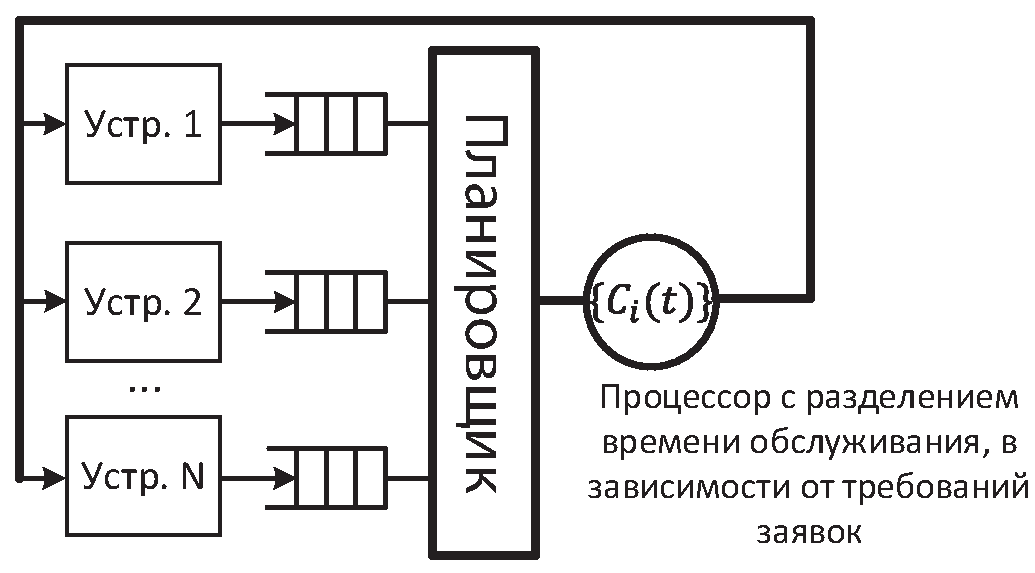
\includegraphics[width=0.6\textwidth]{Chapter2/QnModel.pdf}
\caption{Система передачи видеоданных как замкнутая система массового обслуживания}
\label{fig:QnModel}
\end{center}
\end{figure}

Однако, существует несколько важных отличий систем передачи видеоданных от замкнутых СМО с конечным числом абонентов:
\begin{itemize}
	\item Размер загружаемых сегментов видеоданных изменяется во времени и зависит от скорости загрузки данных, и как следствие, алгоритма планирования;
	\item Длительность интервала времени между получением сегмента и отправки нового запроса не распределено по экспоненциальному закону;
	\item Время передачи сегмента видео через базовую станцию (\textit{время обслуживания заявки}) зависит от его размера и характеристик беспроводного канала всех активных абонентов в текущий момент времени (изменяемая интенсивность обслуживания во времени с дополнительной зависимостью от предыстории).
\end{itemize}

%Данные отличия приводят к невозможности анализа системы передачи видеоданных методами, используемых при анализе классических СМО.

\section{Взаимосвязь характеристик беспроводной централизованной сети и воспроизведения видеоданных}
\label{chap2:InterrelationVideoParams}

Представленная ранее аналитическая модель описывает важнейшие компоненты и параметры реальной системы передачи видеоданных. Основываясь на данной модели вводится утверждение~\ref{lem:GeneralConstrain}, описывающая основные взаимосвязи между параметрами системы.

\begin{lemma}
\label{lem:GeneralConstrain}
Для всевозможных алгоритмов планирования и адаптации видеоряда, удовлетворяющих допущениям, представленных в подразделе \ref{chap2:Scheduler}, следующее неравенство истинно:
\emph{
\begin{equation}
	\label{eq:GeneralConstrain}
	\sum\limits_{i=1}^{N} {\left(1-\nu^R_i\nu^C_i\right)\frac{E[R_i]E[C_i^{-1}]}{q_i + \gamma_i}} \leq 1.
\end{equation}
}
\end{lemma}
В неравенстве (\ref{eq:GeneralConstrain}) обозначения $q_i$, $\gamma_i$, $\nu^R_i$ соответствуют определениям \ref{def:BWTR}, \ref{def:VideoSparseness} и выражению \ref{eq:SwitchRatio} соответственно. $\nu^C_i$~--~коэффициент вариации максимально достижимой скорости канала пользователя $i$.
%
%~--~отношение длительностей буферизации и просмотра пользователя $i$ (определение \ref{def:BWTR}), $\gamma_i$~--~коэффициент разреженности видеопотока (определение \ref{def:VideoSparseness}), $\nu^R_i$~--~верхняя граница коэффициента вариации битовой скорости просматриваемых видеороликов пользователя $i$, .
%
\begin{proof}
Рассмотрим процессы в системе передачи видеоданных, когда некоторый пользователь $i$ загружает пакет $k$ из сегмента $j$. В течение загрузки пакета через систему был передан следующий объем данных $\frac{R_{i,j} d }{P_{i,j}}$, который может быть вычислен исходя из наблюдения за скоростью передачи данных в беспроводном канале:
\begin{equation}
	\nonumber
	\int\limits_{t_{i,j,k}}^{t_{i,j,k} + \Delta t_{i,j,k}} S_i(t) dt = C_{i,j,k} \int\limits_{t_{i,j,k}}^{t_{i,j,k} + \Delta t_{i,j,k}}\alpha_i(t) dt = \frac{R_{i,j} d }{P_{i,j}},
\end{equation}
где $t_{i,j,k}$~--~момент времени начала загрузки пользователем $i$ пакета под номером $k$ из сегмента $j$, $\Delta t_{i,j,k}$~--~длительность загрузки пользователем $i$ пакета под номером $k$ из сегмента $j$

Перенесем $C_{i,j,k}$ в правую часть последнего равенства и получим долю времени использования канала пользователем $i$ при загрузке $k$-го пакета:
\begin{equation}
	\nonumber
	\int\limits_{t_{i,j,k}}^{t_{i,j,k} + \Delta t_{i,j,k}}\alpha_i(t) dt = \frac{R_{i,j} d }{P_{i,j}}\frac{1}{C_{i,j,k}}.
\end{equation}
Просуммируем левую и правую часть по всем пакетам в сегменте, получим долю времени использования канала пользователем $i$ при загрузке $j$-го сегмента:
\begin{equation}
	\nonumber
	\int\limits_{t_{i,j}}^{t_{i,j} + \Delta t_{i,j}}\alpha_i(t) dt = R_{i,j} d\left( \frac{1}{P_{i,j}}\sum\limits_{k=1}^{P_{i,j}} \frac{1}{C_{i,j,k}}\right),
\end{equation}
где $t_{i,j} = t_{i,j,1}$~--~момент времени начала загрузки пользователем $i$ сегмента $j$, $\Delta t_{i,j} = \sum_{k = 1}^{P_{i,j}} \Delta t_{i,j,k}$~--~длительность загрузки пользователем $i$ сегмента $j$. Согласно введенным ранее обозначениям (подраздел~\ref{chap2:RadioChannel}) $C_{i,j}^{-1} = P_{i,j}^{-1}\sum_{k=1}^{P_{i,j}} C_{i,j,k}^{-1}$, тогда выражение примет вид:
\begin{equation}
	\nonumber
	\int\limits_{t_{i,j}}^{t_{i,j} + \Delta t_{i,j}}\alpha_i(t) dt = R_{i,j}C_{i,j}^{-1} d.
\end{equation}

%Важно отметить, что в реальной системе величина $P_{i,j}$ принимает значения большие 75-ти. Например, в соответствие с таблицей~\ref{tab:youtubeBr}, для обеспечения разрешения 360p на мобильном устройстве необходима битовая скорость потока $0.45$ Мб/c, минимальная длительность сегмента видеоданных $2$ секунды (таблица~\ref{tab:DashJSParams}), максимальный размер пакета, который может быть передан без фрагментации $1440$ байт. Следовательно, размер одного сегмента $112500$ байт, и он может быть передан за $79$ пакетов. Таким образом, если $C^{-1}_{i,1,1}, C^{-1}_{i,1,2}, \ldots,$ $ C^{-1}_{i,2,1}, C^{-1}_{i,2,2}, \ldots$ формирует эргодический случайный процесс с конечными математическим ожиданием $E[C_i^{-1}]$ и коэффициентом вариации (подраздел~\ref{chap2:Assumptions}), то значение $C_{i,j}^{-1} = E[C_i^{-1}]$.

Тогда доля времени использования канала пользователем $i$ за время $T$:
\begin{equation}
	\label{eq:lemma_1}
	\int\limits_{0}^{T}\alpha_i(t) dt = d\sum\limits_{j=1}^{H_i^T}R_{i,j}C_{i,j}^{-1} + \Delta s_i,
\end{equation}
где $H_i^T$~--~число полностью загруженных сегментов пользователем $i$ в течении времени $T$, $\Delta s_i$~--~длительность видео, загруженного пользователем $i$, но не воспроизведенный плеером. Просуммировав уравнение~(\ref{eq:lemma_1}) для всех пользователей в системе ($i=\overline{1,N}$) и внеся сумму под знак интеграла было получено следующее выражение:
\begin{equation}
	\nonumber
	\int\limits_{0}^{T}\sum\limits_{i=1}^{N}\alpha_i(t)dt = \sum\limits_{i=1}^{N}d\sum\limits_{j=1}^{H_i^T}R_{i,j}C_{i,j}^{-1} + \Delta s,
\end{equation}
где $\Delta s = \sum\limits_{i=1}^{N} \Delta s_i$.

Так как в каждый момент времени $t$ сумма выделенных ресурсов не может превышать единицы, согласно условию (\ref{eq:AllResources}), следовательно $\int\limits_{0}^{T}\sum\limits_{i=1}^{N}\alpha_i(t)dt \leq T$:
\begin{equation}
	\nonumber
	d\sum\limits_{i=1}^{N}\sum\limits_{j=1}^{H_i^T}R_{i,j}C_{i,j}^{-1} + \Delta s \leq T.
\end{equation}
Разделим левую и правую часть неравенства на $T$ и внесем его под первый знак суммы, так как $T>0$ знак неравенства не изменится.
\begin{equation}
	\nonumber
	\sum\limits_{i=1}^{N}{\frac{d\sum\limits_{j=1}^{H_i^T}R_{i,j}C_{i,j}^{-1} + \Delta s_i}{T}} \leq 1.
\end{equation}
Для каждого пользователя время пребывание в системе состоит из буферизаций, просмотров и пауз между просмотрами видео: $T = b_i^T + w_i^T + p_i^T $, следовательно, последнее неравенство представляется в следующем виде:
\begin{equation}
	\nonumber
	 \sum\limits_{i=1}^{N}{\frac{d\sum\limits_{j=1}^{H_i^T}R_{i,j}C_{i,j}^{-1} + \Delta s_i}{b_i^T + w_i^T + p_i^T}} \leq 1.
\end{equation}
Так как длительность просмотра равняется длительности всех загруженных сегментов, $w_i^T = H_i^T d,i=\overline{1,N}$:
\begin{equation}
	\nonumber
	\sum\limits_{i=1}^{N}\frac{w_i^T \frac{1}{H_i^T}\sum\limits_{j=1}^{H_i^T}R_{i,j}C_{i,j}^{-1} + \Delta s_i}{b_i^T + w_i^T + p_i^T} \leq 1.
\end{equation}
Разделив числитель и знаменатель левой части полученного выражения на $w_i^T$ и устремим время в бесконечность ($T\rightarrow\infty$). Для каждого абонента $i = \overline{1,N}$ воспользуемся определением $q_i$ и получим следующее выражение:
\begin{equation}
	\nonumber
	\sum\limits_{i=1}^{N}\frac{E\left[R_{i}C_{i}^{-1}\right] }{q_i + \gamma_i} \leq 1.
\end{equation}
Данный переход возможен так как последовательности $R_{i,1}, R_{i,2}, \ldots$ и $C_{i,1}, C_{i,2}, \ldots i=\overline{1,N}$ формируют эргодические случайные процессы с кончеными первыми двумя моментами (подраздел~\ref{chap2:Assumptions}).

Рассмотрим более подробно значение, получившее в числителе: $E\left[R_{i}C_{i}^{-1}\right]$. Важно отметить, что битовая скорость потока $R_i$ для каждого пользователя выбирается в зависимости от оценки качества канала, которая определяется максимально достижимой скоростью канала $C_i$. Следовательно, значения $R_i$ и $C_i$ являются зависимыми величинами, и математическое ожидание их произведения:
\begin{equation}
	\nonumber
	E\left[R_{i}C_{i}^{-1}\right] = E\left[R_{i}\right]E\left[C_{i}^{-1}\right] + r \left(R_i, C_{i}^{-1}\right) \sigma[R_i]\sigma[C_i^{-1}],
\end{equation}
где $r \left(R_i, C_{i}^{-1}\right)$ является коэффициентом корреляции между величинами $R_i$ и $C_{i}^{-1}$. По определению значение $r \left(R_i, C_{i}^{-1}\right)$ принимает значения в отрезке $[-1, 1]$, следовательно:
\begin{equation}
	\nonumber
	 E\left[R_{i}\right]E\left[C_{i}^{-1}\right] - \sigma[R_i]\sigma[C_i^{-1}] \leq E\left[R_{i}C_{i}^{-1}\right].
\end{equation}
Исходя из данного факта:
\begin{equation}
	\nonumber
	\sum\limits_{i=1}^{N} {\left(1-\nu^R_i\nu^C_i\right)\frac{E[R_i]E[C_i^{-1}]}{q_i + \gamma_i}} \leq 1.
\end{equation}
Таким образом, утверждение \ref{lem:GeneralConstrain} доказано.
\end{proof}

Результат, представленный в утверждении \ref{lem:GeneralConstrain}, описывает взаимосвязь между всеми характеристиками сети передачи видеоданных от особенностей модели поведения пользователя ($\gamma_i$, $q_i$) и характеристик видеопотока ($E[R_i]$), до аспектов работы радиоканала ($E[C_i^{-1}]$) для всех пользователей в сети. Полученное выражение возможно использовать в качестве ограничения на достижимый объем ресурсов радиоканала при оптимизации передачи видеоданных в беспроводных централизованных сетях.

Для упрощения математических выкладок в качестве обозначений $E[R_i]$ и $E[C^{-1}_i]$ будут использоваться обозначение $\tilde{R}_i$ и $\tilde{C}^{-1}_i$ соответственно.

\section{Выводы по разделу}

В данном разделе была предложена модель передачи видеоданных в современных централизованных беспроводных сетях. Предложенная модель описывает все важнейшие компоненты существующих сетей: магистральная и опорная сети передачи данных, базовая станция (структура беспроводного канала и алгоритм распределения его ресурсов) модель видеотрафика (формат представления видео и аспекты работы воспроизводящего устройства). Так же модель системы передачи видеоданных в беспроводных централизованных сетях была рассмотрена как замкнутая система массового обслуживания с конечным числом абонентов. В завершении раздела был представлен результат, описывающий основополагающие взаимосвязи между всеми характеристиками сети передачи видеоданных.

Основные результаты раздела возможно сформулировать следующим образом:
\begin{itemize}
	\item Предложена модель передачи видеоданных в беспроводных централизованных сетях, включающая в себя:
	\begin{itemize}
		\item Модель опорной и магистральной сети передачи данных (подраздел~\ref{chap2:GeneralOverview});
		\item Модель беспроводного канала связи (подраздел~\ref{chap2:RadioChannel});
		\item Модель работы базовой станции и планировщика ресурсов беспроводного канала (подраздел~\ref{chap2:Scheduler});
		\item Модель воспроизводящего устройства и видеотрафика (подраздел~\ref{chap2:VideoTrafficModel});
		\item Систему допущений (подраздел~\ref{chap2:Assumptions}).
	\end{itemize}
	\item Проведен анализ беспроводных систем перечи видео как замкнутых систем массового обслуживания с конечным числом абонентов (подраздел~\ref{chap2:QueuningNetwork});
	\item Представлена взаимосвязь между характеристиками сети передачи видеоданных (подраздел~\ref{chap2:InterrelationVideoParams}).
\end{itemize}           % Раздел 2
\chapter{ИССЛЕДОВАНИЕ ПРОИЗВОДИТЕЛЬНОСТИ БЕСПРОВОДНЫХ ЦЕНТРАЛИЗОВАННЫХ СЕТЕЙ ДЛЯ ПЕРЕДАЧИ НЕАДАПТИВНЫХ ВИДЕОПОТОКОВ}
\label{chap3}

\section{Вводные замечания}
\label{chap3:Intro}
В настоящее время в беспроводных сетях, несмотря на бурное развитие технологий адаптивной передачи видеоконтента, достаточно распространена передача видео с использованием неадаптивных видеоплееров. Наиболее ярким примером является социальная сеть Facebook, весь видеоконтент которой представлен в двух репрезентациях: стандартном и высоком разрешениях, в англоязычной терминологии Standard Definition и High Definition соотвественно. Пользователь, при просмотре видео, может выбрать один из двух представленных выше вариантов качества видеопотока и оно не будет изменяться во времени. Подобная модель поведения абсолютно соотвествует описанию неадаптивного видеоплеера, представленного в подразделе~\ref{chap1:VideoPlayers}.

В настоящем разделе производится аналитическое исследование производительности беспроводных централизованных систем передачи информации с доминированием передачи видеоданных по протоколу прикладного уровня HTTP. В начале раздела предлагается критерий качества обслуживания для неадаптивных видеопотоков. Далее вводится дополнительные допущения, специфичные для неадаптивных видеопоследовательностей. Затем формулируется оптимизационная задача и предлагается нижняя граница для введенного критерия качества обслуживания. В завершении предлагается численный пример, демонстрирующий производительность стандартных алгоритмов планирования распределения ресурсов беспроводного канала по сравнению с полученной нижней границей.

Основные результаты данного раздела опубликованы в работах~\cite{past_tur,Suai2017}.

\section{Критерий качества восприятия неадаптивного видеопотока}
\label{chap3:NonAdaptiveQoe}
Обобщая информацию, представленную ранее в настоящей работе, можно выделить три основных фактора, влияющих на восприятие видеопоследовательности:
\begin{itemize}
	\item Репрезентация (рекомендуемое разрешение экрана и частота кадров видео), определяемая битовой скоростью потока (подраздел~\ref{chap1:VideoMOS}).
	\item Прерывание воспроизведения, вызванное буферизацией видеопотока, включающее начальную буферизацию видео (подраздел~\ref{chap1:VideoMOS});
	\item Гладкость воспроизведения видеопоследовательности~--~частота изменения битовой скорости во времени (подраздел~\ref{chap2:VideoTrafficModel}).
\end{itemize}
Произведем рассмотрение каждого из перечисленных выше факторов с точки зрения неадаптивных видеопоследовательностей.

При работе неадаптивного видеоплеера решение о выборе репрезентации видеоряда принимает пользователь некоторым образом, отвечающим индивидуальным требованиям к качеству просматриваемого видео и не изменяет его во времени. На основе факта о неизменности репрезентации видео во времени, следует что гладкость воспроизведения, которая характеризует частоту изменения репрезентации во времени, не влияет на качество восприятия видеоряда.

Таким образом, на удовлетворенность пользователя от просмотра неадаптивных видеопоследовательностей влияют прерывания воспроизведения, вызванные опустошением буфера и начальной буферизацией на пользовательском устройстве.

Очевидно, что если в соте находится большое число абонентов, то могут проявится эффекты деградации воспроизведения видео у пользователей, ввиду конечности количества частотно-временных ресурсов беспроводного канала и ограниченности снизу минимальной битовой скорости репрезентации видео. Например, если некоторому пользователю базовая станция обеспечивает скорость загрузки информации равную $0.25$ Мбит/с, а битовая скорость минимальной репрезентации равняется $0.5$ Мбит/с, то у данного пользователя при просмотре видео с высокой вероятностью будет длительная начальная буферизация и неизбежно возникнут прерывания воспроизведения видео. Основываясь на данном факте введем определение перегрузки:
\begin{definition}
\label{def:Congestion}
    \emph{Перегрузка}~--~состояние системы передачи информации, характеризующее недостаток ресурсов для обеспечения достаточного уровня удовлетворенности всех активных пользователей.
\end{definition}

Как было представлено в подразделе~\ref{chap2:GeneralOverview}, все время $T$ нахождения пользователя в системе разделено на три: буферизация $\left( b_i^T \right)$, просмотр $\left( w_i^T \right)$ и паузы между просмотрами видео $\left( p_i^T \right)$. В настоящем разделе предлагается оценивать качество восприятия видеопотока для пользователя как нормированное отношение длительности буферизации к просмотру за время $T$:
\begin{definition}
\label{def:gMetric}
    \emph{Нормированное отношение длительности буферизации к просмотру} для пользователя $i$~--~это отношение общей длительности ожидания к длительности времени нахождения пользователя в системе, исключая паузы между просмотрами видео:
    \emph{
    \begin{equation}
    	\label{eq:gMetric}
		g_i = \lim\limits_{T\rightarrow\infty} \frac{b_i^T}{w_i^T + b_i^T}.
	\end{equation}
	}
\end{definition}

Критерий восприятия (\ref{eq:gMetric}) описывает процентное соотношение общих длительностей буферизации и просмотра для пользователя $i$ за время $T$. На основе данного критерия возможно оценить удовлетворенность пользователя следующим образом:
$$g_i=
\begin{cases}
0, & \text{пользователь $i$ удовлетворен просмотром}\\
(0,1) & \text{пользователь $i$ наблюдает негативные эффекты при просмотре}\\
1, & \text{пользователь $i$ полностью неудовлетворен просмотром}\\
\end{cases}.
$$
Если пользователь не ожидал в течение времени $\left(b_i^T = 0\right)$, тогда значение $g_i = 0$.
Если пользователь, за время $T$, не просмотрел ни одной секунды видео $\left(w_i^T = 0\right)$, то значение $g_i$ будет равно $1$. Изначально критерий \ref{def:gMetric} был предложен в работе \cite{QoE_enhancement}, в англоязычной литературе данный критерий известен под названием \textit{<<rebuffering percentage>>}. Термин \textit{<<rebuffering>>} в англоязычной литературе используется для обозначения времени ожидания воспроизведения в течении просмотра видео при передаче с использованием протокола HTTP.

В качестве критерия качества работы системы в целом предлагается использовать среднее значение отношение длительности буферизации к просмотру по всем пользователям, присутствующих в системе: $\bar{g}\left(\mathcal{A}\right)$. Важно отметить, что значение критерия качества обслуживания имеет прямую зависимость от алгоритма планирования распределения ресурсов беспроводного канала $\mathcal{A}(\cdot)$.

После определения критерия качества обслуживания в дальнейшем будет произведена постановка оптимизационной задачи.

\section{Постановка оптимизационной задачи}
\label{chap3:NonAdaptiveOptimizationProblem}

В настоящем подразделе будет продолжено рассмотрение критерия качества обслуживания для неадаптивных видеопотоков, введенного в подразделе~\ref{chap3:NonAdaptiveQoe}. На основе проведенного рассмотрения будет предложена постановка оптимизационной задачи, решение которой характеризует максимальную возможную производительность алгоритма планирования при передаче неадаптивных видеопотоков.

Рассмотрим критерий качества для неадаптивного видео: нормированного отношения длительности буферизации к просмотру $g_i$ (\ref{def:gMetric}). По определению, удовлетворенность пользователя имеет обратную корреляцию с данным критерием: чем меньше значение $g_i$, тем выше удовлетворенность пользователя $i$. Для каждого конкретного алгоритма планирования $A$, принадлежащему множеству $\mathcal{A}(\cdot)$, производительность возможно оценить следующим образом:
%Как следствие, основной целью увеличения производительности системы является поиск минимального значения $\bar{g}$ по всем возможным алгоритмам планирования $\mathcal{A}(\cdot)$, удовлетворяющих введенным допущениям: 
$$\bar{g}\left(A\right) = \frac{1}{N}\left(\sum\limits_{i=1}^{N} {g_i\left(A\right)}\right).$$

Однако, множество возможных алгоритмов планирования, удовлетворяющих допущениям, является бесконечным и несчетным, поэтому вместо поиска минимального значения в данном разделе будет найдена нижняя граница (инфинум) по всем возможным алгоритмам $\mathcal{A}(\cdot)$:

\begin{equation}
	\label{eq:gMetricGoal}
	G = \inf\limits_{A \in \mathcal{A}} \bar{g}\left(A\right).
\end{equation}

Ранее в подразделе~\ref{chap2:GeneralOverview} было введено определение для $q_i$: отношения времени буферизации к просмотру для пользователя $i$ (определение~\ref{def:BWTR}). Покажем, каким образом взаимосвязаны значения $g_i$ и $q_i$. По определению данных величин, если продолжительность буферизации пользователя $i$ за время $T$ $\left(b_i^T\right)$ равнялась нулю, то $q_i=g_i=0$. Пусть значение $\left(b_i^T\right)$ отлично от нуля, тогда значения $q_i$ и $g_i$ взаимосвязаны следующим образом:
$$q_i = \frac{g_i}{1-g_i}.$$

На основе представленной выше взаимосвязи значений критериев качества обслуживания выражение (\ref{eq:GeneralConstrain}), полученное в результате доказательства Утверждения~\ref{lem:GeneralConstrain} (подраздел \ref{chap2:InterrelationVideoParams}) примет следующий вид:
\begin{equation}
	\label{eq:GeneralConstrainToG}
	\sum\limits_{i=1}^{N} {\left(1-\nu^R_i\nu^C_i\right)E[R_i]E[C_i^{-1}]\frac{1-g_i}{g_i + \gamma_i (1-g_i)}} \leq 1.
\end{equation}

При просмотре неадаптивных видеопоследовательностей пользователь $i$ в начальный момент времени выбирает репрезентацию с битовой скоростью $R_i$, качество которой его полностью удовлетворяет, и не изменят ее в течении всего времени работы. Данный факт приводит к изменению допущения \textit{Модели видеоплеера} номер $1$ , представленному в подразделе \ref{chap2:Assumptions}, следующим образом:

$1.$   Значение битовой скорости видеопотока для каждого конкретного абонента неизменно во времени: $R_{i,1} = R_{i,2} = \ldots = R_i, i=\overline{1,N}$.

Следствием из данного допущения является равенство коэффициента вариации $\nu^R_i, i=\overline{1,N}$ нулю, а математическое ожидания битовой скорости $E[R_i]$ равно $R_i$ для каждого пользователя $i$. Таким образом, неравенство (\ref{eq:GeneralConstrainToG}) принимает следующий вид:
$$\sum\limits_{i=1}^{N} {R_i E[C_i^{-1}]\frac{1-g_i}{g_i + \gamma_i (1-g_i)}} \leq 1.$$

Для уменьшения объема последующих математических преобразований введем обозначение $K_i$ как $R_i E[C_i^{-1}]$. Важно отметить, что значение $K_i$ не является переменной, так как его компоненты задаются независимыми от оптимизации факторами: пожеланиями пользователя ($R_i$) и условиями беспроводного канала ($E[C_i^{-1}]$).

В дополнении к системе допущений \textit{Модели поведения пользователя при просмотре видео}, введенному в подразделе \ref{chap2:Assumptions}, в рамках настоящего раздела вводится дополнительное допущение:

$2.$   Коэффициент разряженности видеопотока $\gamma_i$ (определение \ref{def:VideoSparseness}) для всех пользователей имеет равное значение: $\gamma_i = \gamma, i=\overline{1,N}$.

Настоящее допущение обусловлено зависимостью в реальной системе между длительностью видеоролика и паузы после его просмотра: после просмотра длительного ролика пользователь <<осмысливает>> его более длительный промежуток времени, чем при просмотре короткого ролика. Данный факт приводит приблизительному равенству коэффициентов разряженности потока у всех пользователей.

Обобщая сказанное выше, в настоящем разделе предлагается оптимизационная задача следующего вида:
\begin{equation}
\begin{array}{l}
\text{ \textbf{Минимизировать:} } G = \sum\limits_{i=1}^{N} {g_i} \\
\text{ \textbf{При условии:} }\\
\begin{cases}
\sum\limits_{i=1}^{N} {\frac{K_i (1-g_i)}{g_i + \gamma (1-g_i)}} \leq 1 \\
g_i \in [0,1], i=\overline{1,N}
\end{cases}
\end{array}.
\label{eq:optim_problem_g}
\end{equation}

Оптимизационная задача (\ref{eq:optim_problem_g}) является задачей нелинейного программирования, ввиду нелинейности первого ограничения. Дальнейшая часть данного раздела посвящена поиску оптимального решения задачи (\ref{eq:optim_problem_g}), значение которого задает нижнюю границу по всем возможным алгоритмам планирования, удовлетворяющих допущениям введенных в подразделе ~\ref{chap2:Assumptions}.

\section{Решение обобщенной задачи о непрерывном рюкзаке}
\label{chap3:GeneralizedFKSP}

Отыскание решения оптимизационной задачи (\ref{eq:optim_problem_g}) является сложной задачей, и для ее решения необходимо проделать несколько шагов. Изначально будет рассмотрено обобщение известной задачи о непрерывном рюкзаке и найдено его решение. Далее будет показано, каким образом найденное решение может быть использовано при решении оптимизационной задачи (\ref{eq:optim_problem_g}). В данном подразделе рассматривается задача о непрерывном рюкзаке, ее обобщение и находится находится решение обобщенной задачи о непрерывном рюкзаке.

Представленное ниже решение опубликовано в работе \cite{Suai2017}.

Задача о непрерывном рюкзаке в англоязычной литературе известна под термином \textit{<<fractional knapsack problem>>}, и подробно описана в \cite{Cormen:2009:IAT:1614191}. Задача формулируется следующим образом. Имеется набор из $N$ предметов, каждый предмет $i$ характеризуется двумя величинами: стоимостью $(c_i)$ и весом ($w_i$). Также имеется рюкзак неограниченного объема, характеризующийся с весом предметов, помещенных в него. Считается, что человек, который будет нести этот рюкзак, не может поднять вес превышающий $W$. Все предметы считаются делимыми на бесконечное число частей, что позволяет выбрать долю каждого предмета $x_i$, которую он положит в рюкзак. В качестве задачи, предлагается найти такой вектор $(x_1, x_2, \ldots, x_N)$, что вес взятых долей предметов не превышает $W$ и при этом стоимость взятых предметов максимальна. Математическое представление задачи о непрерывном рюкзаке представлено системой (\ref{eq:fksp}):

\begin{equation}
\begin{array}{l}
\text{ \textbf{Максимизировать:} } \sum\limits_{i=1}^{N} {c_i x_i} \\
\text{ \textbf{При условии:} }\\
\begin{cases}
\sum\limits_{i=1}^{N} {w_i x_i} \leq W \\
x_i \in \left[0,1\right], & i=\overline{1,N}
\end{cases}
\end{array}.
\label{eq:fksp}
\end{equation}
Таким образом задача о непрерывном рюкзаке относится к классу непрерывных задач линейного программирования от нескольких переменных.

Важным отличием задачи о непрерывном рюкзаке (\ref{eq:fksp}), от классической задачи о рюкзаке (\textit{<<0-1 knapsack problem>>}) заключается в возможности деления предметов, когда в классической задаче предметы считаются неделимыми (величина $x_i$ может принимать только два значения: $0$ и $1$). Известно, что задача о рюкзаке не имеет замкнутого решения и может быть решена методами динамического программирования. Однако, для задачи о непрерывном рюкзаке оптимальное решение может быть получено <<жадным алгоритмом>>:

\begin{algorithm}
  \caption{: Решение задачи о непрерывном рюкзаке}
	\label{alg:algorithm_lemma}
  \begin{algorithmic}[1]
	 \item Сортировка предметов по возрастанию отношений $\frac{w_i}{c_i}$, и их нумерация, в соответствие с сортировкой;
	 \item Нахождение предмета с индексом $j:\begin{cases}
		\sum\limits_{i=1}^{j-1} {w_i} \leq W \\
		\sum\limits_{i=1}^{j} {w_i} > W
		\end{cases}$
		\newline
		Если $j\in\varnothing, j=N+1$;
	\item Нахождение оптимальных значений $x_i$: \newline
	$x_i=\begin{cases}
		1, & i < j \\
		\frac{1}{w_j}\left(W - \sum\limits_{i=1}^{j-1} {w_i}\right), & i=j \\
		0, & i > j
		\end{cases}$.
  \end{algorithmic}
\end{algorithm}

Дальнейшее повествование в настоящем подразделе будет построено следующим образом. Первым шагом, будет представлено общение задачи о непрерывном рюкзаке. Вторым шагом будет показано каким образом алгоритм \ref{alg:algorithm_lemma} может быть применен для решения обобщенной задачи о непрерывном рюкзаке. В завершении подраздела будет представлено сравнение сложности полученного решения со стандартными методами решения задач выпуклого программирования от нескольких переменных.

Обобщение задачи о непрерывном рюкзаке:
\begin{equation}
\begin{array}{l}
\text{ \textbf{Максимизировать:} } \sum\limits_{i=1}^{N} {f(x_i)} \\
\text{ \textbf{При условии:} }\\
\begin{cases}
\sum\limits_{i=1}^{N} {w_i x_i} \leq W \\
x_i \in \left[0,1\right], & i=\overline{1,N}
\end{cases}
\end{array},
\label{eq:fksp_general}
\end{equation}
где $f(x_i)$~--~непрерывная, дважды дифференцируемая, строго монотонно возрастающая, выпуклая вниз функция, ограниченная сверху и снизу в области определения $x_i$.

Оптимизационная задача (\ref{eq:fksp_general}) относится к классу выпуклого программирования от нескольких переменных с ограничениями типа неравенства. Важно отметить факт, что задачи выпуклого программирования являются подклассом задач нелинейного программирования.

Решение оптимизационной задачи (\ref{eq:fksp_general}) описывается в утверждении \ref{lem:fksp_general_lemma}.

\begin{lemma}
\label{lem:fksp_general_lemma}
Если в алгоритме \ref{alg:algorithm_lemma} принять $\forall i: c_i = 1$, то вектор $X = (x_1, x_2, \ldots, x_N)$, полученный в результате выполнения алгоритма \ref{alg:algorithm_lemma}, является оптимальным решением задачи нелинейного программирования (\ref{eq:fksp_general}).
\end{lemma}

\begin{proof}

В основе предложенного далее доказательства был использован метод от противного. Предположим, что существует оптимальное решение $Y = (y_1, y_2, \ldots, y_N)$, удовлетворяющее всем ограничениям системы (\ref{eq:fksp_general}), отличное от решения $X = (x_1, x_2, \ldots, x_N)$, полученного на основе алгоритма \ref{alg:algorithm_lemma} (рисунок~\ref{fig:X_Y_Solutions}). Важно отметить, что нумерация всех предметов происходит в порядке сортировки на шаге $1$ алгоритма \ref{alg:algorithm_lemma}. Тогда в решении $Y$ найдется пара индексов $k$ и $l$ такие что:
\begin{itemize}
	\item $k$~--~наименьший индекс предмета, взятая в рюкзак доля которого меньше единицы: $y_k < 1$;
	\item $l$~--~наименьший индекс предмета, больший $k$, взятая в рюкзак доля которого отлична от нуля: $y_l > 0, l>k$.
\end{itemize}

\begin{figure}[htbp]
\begin{center}
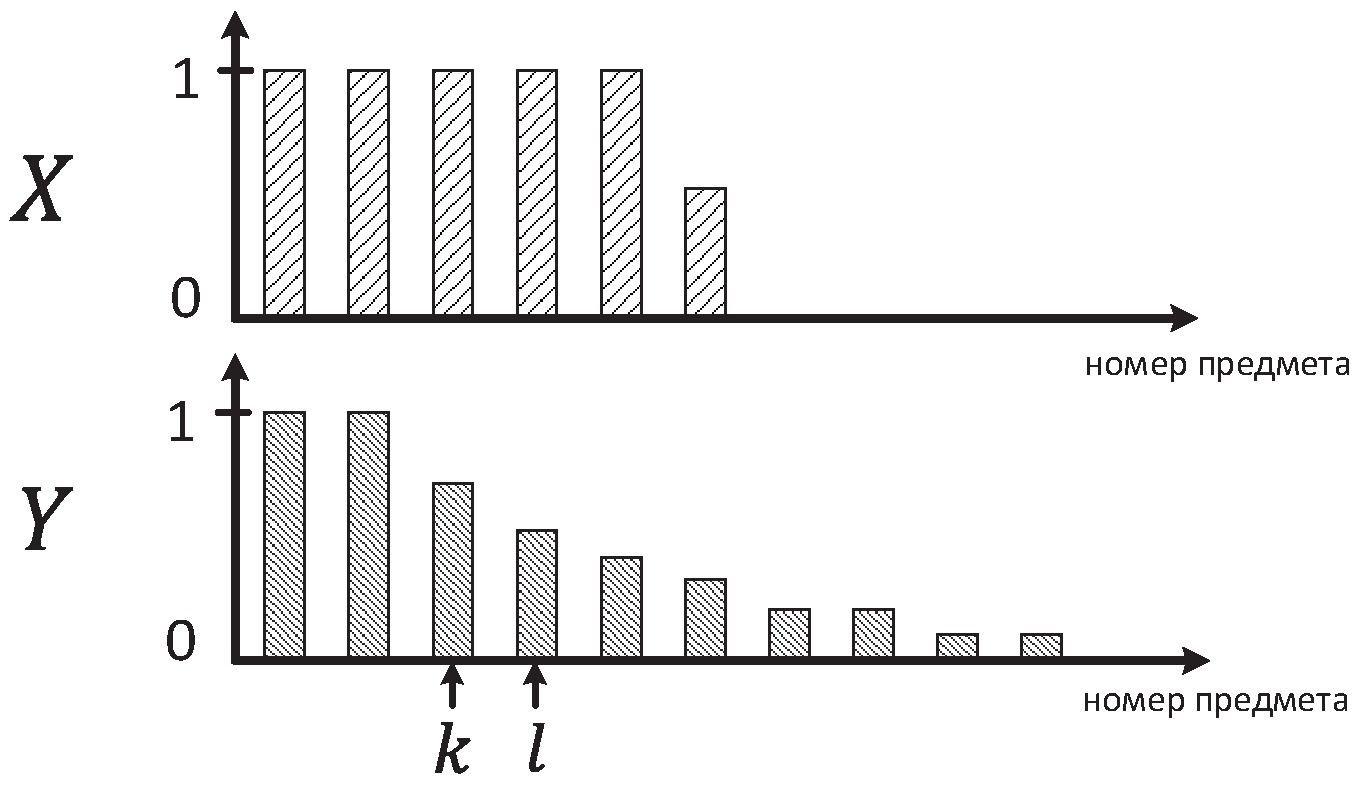
\includegraphics[width=0.6\textwidth]{Chapter3/X_Y.pdf}
\caption{Вид решений $X$ и $Y$}
\label{fig:X_Y_Solutions}
\end{center}
\end{figure}

Покажем, каким образом возможно перераспределить доли взятых предметов $y_k$ и $y_l$ под индексами $k$ и $l$ соответственно, для максимизации целевой функции системы (\ref{eq:fksp_general}).

Для этого введем следующие обозначения:
\begin{itemize}
	\item $w_{s}$~--~суммарный вес взятых предметов $k$ и $l$: $$w_{s} = y_k w_k + y_l w_l.$$ Так как значение $y_k < 1$ и $y_l \in (0, 1]$, то $w_{s} < w_k + w_l$.
	\item Обновленное решение $Y^{*}$: $$Y^{*}=(y_1, \ldots, y_{k-1}, y_k^{*}, y_{k+1}, \ldots, y_{l-1}, y_l^{*}, y_{l+1}, \ldots),$$ где $y_k^{*}$ и $y_l^{*}$~--~обновленные доли предметов под индексами $k$ и $l$ соответственно.
\end{itemize}

Решения $Y$ и $Y^{*}$ удовлетворяют ограничениям оптимизационной задачи (\ref{eq:fksp_general}) и отличаются только в долях предметов под индексами $k$ и $l$. Далее в настоящем доказательстве, будет показано, что за счет преобразования долей $y_k$ и $y_l$ (решение $Y$) в $y_k^{*}$ и $y_l^{*}$ (решение $Y^{*}$) соответственно, и без изменения остальных значений долей предметов возможно увеличить значение целевой функции задачи (\ref{eq:fksp_general}). То есть будет показано, что для любого решения $Y$ найдется решение $Y^{*}$, отличное в позициях $k$ и $l$, такое что целевая функция при решении $Y^{*}$ больше, чем при $Y$.

Для этого поставим промежуточную оптимизационную задачу:
\begin{equation}
\begin{array}{l}
\text{ \textbf{Максимизировать:} } f(y_k^{*}) + f(y_l^{*}) \\
\text{ \textbf{При условии:} }\\
\begin{cases}
w_{s} = y_k^{*} w_k + y_l^{*} w_l \\
w_s < w_k + w_l \\
w_k < w_l \\
y_k^{*},y_l^{*} \in [0,1]
\end{cases}
\end{array}.
\label{eq:inter_proof_fksp_lemma}
\end{equation}

В промежуточной оптимизационной задаче (\ref{eq:inter_proof_fksp_lemma}) целевая функция состоит из суммы функций $f(\cdot)$ для долей предметов $k$ и $l$, так как решение $Y^{*}$ отлично от $Y$ только в данных позициях. Как следствие, значения остальных элементов суммы являются константами и не влияют на значение целевой функции. В ограничениях задачи (\ref{eq:inter_proof_fksp_lemma}) указывается, что суммарный вес предметов $k$ и $l$ не может быть изменен, а значит не будет нарушено ограничение на суммарный вес всех предметов взятых в рюкзак в системе (\ref{eq:fksp_general}).

Таким образом, целью промежуточной оптимизационной задачи (\ref{eq:inter_proof_fksp_lemma}) является отыскание таких $y_k^{*}$ и $y_l^{*}$, при которых целевая функция задачи (\ref{eq:inter_proof_fksp_lemma}) принимает максимальное значение. Важно отметить, что максимизация целевой функции промежуточной задачи (\ref{eq:inter_proof_fksp_lemma}) приводит и к максимизации целевой функции в обобщенной задаче о непрерывном рюкзаке (\ref{eq:fksp_general}). Следствием этого является факт, что если решение $Y$ может быть улучшено в промежуточной оптимизационной задаче, то оно не является оптимальным решением задачи (\ref{eq:fksp_general}).

Продолжим рассмотрение промежуточной оптимизационной задачи. Из системы (\ref{eq:inter_proof_fksp_lemma}) выразим $y_k^{*}$ как функцию от $y_l^{*}$:
$$y_k^{*} = \frac{w_s - y_l^{*} w_l}{w_k}.$$

Подставим полученный результат в систему (\ref{eq:inter_proof_fksp_lemma}):

\begin{equation}
\begin{array}{l}
\text{ \textbf{Максимизировать:} } f\left(\frac{w_s - y_l^{*} w_l}{w_k}\right) + f(y_l^{*}) \\
\text{ \textbf{При условии:} }\\
\begin{cases}
y_k^{*} = \frac{w_s - y_l^{*} w_l}{w_k}\\
w_s < w_k + w_l \\
w_k < w_l \\
y_k^{*},y_l^{*} \in [0,1]
\end{cases}
\end{array}.
\label{eq:inter_proof_fksp_lemma_upd}
\end{equation}

Найдем вторую производную целевой функции задачи (\ref{eq:inter_proof_fksp_lemma_upd}):
$$\left[f\left(\frac{w_s - y_l^{*} w_l}{w_k}\right) + f(y_l^{*})\right]'' = f''\left(\frac{w_s - y_l^{*} w_l}{w_k}\right) \left(\frac{w_l}{w_k}\right)^2 + f''(y_l^{*}).$$

Так как функция $f(x)$ является выпуклой вниз, то $f''(x) > 0$. Следовательно выражение в правой части является положительным. Обобщая сказанное выше, экстремумом оптимизационной задачи (\ref{eq:inter_proof_fksp_lemma_upd}), если он существует, является минимум, как следствие, максимальное значение целевая функция принимает на граничных значениях $y_l^{*}$ (рисунок~\ref{fig:ObjectiveFunctions}).

\begin{figure}[htbp]
\begin{center}
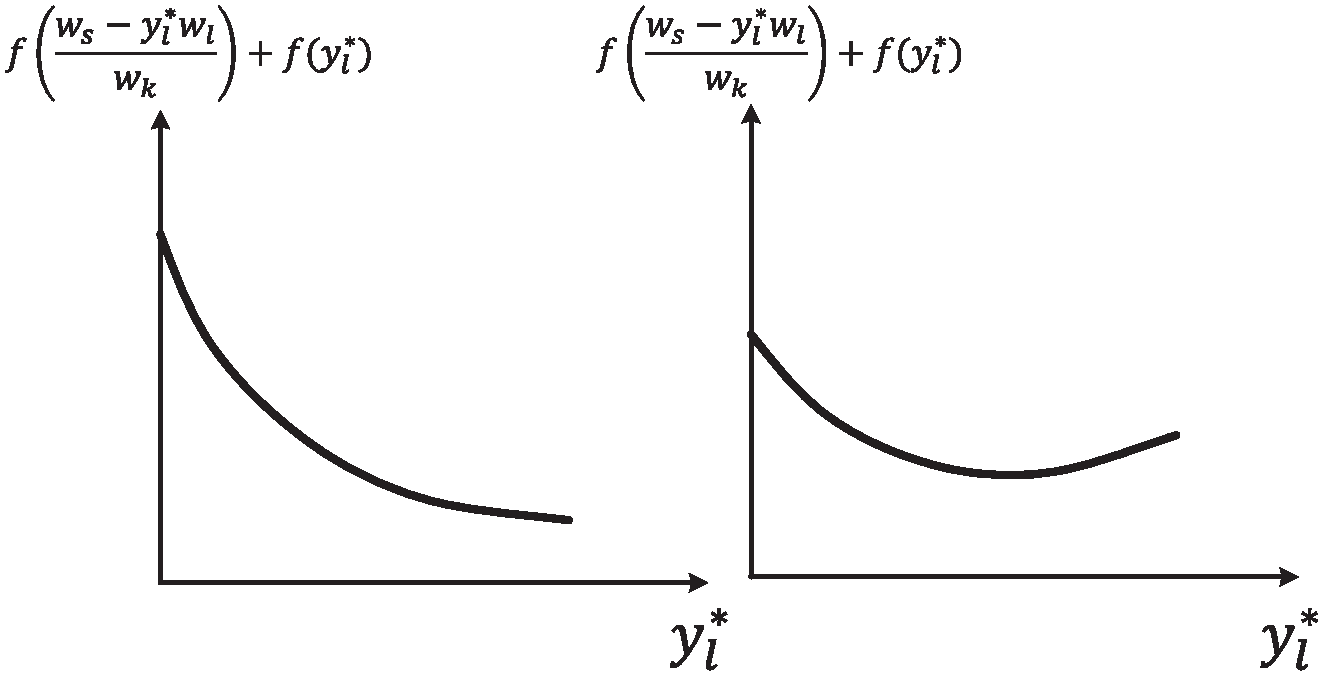
\includegraphics[width=0.8\textwidth]{Chapter3/objective_fuctions.pdf}
\caption{Вид целевой функции промежуточной оптимизационной задачи}
\label{fig:ObjectiveFunctions}
\end{center}
\end{figure}

Будем рассматривать различные ситуации, в зависимости от значения $w_s$. Разобьем все возможные значения $w_s$ на три интервала (рисунок \ref{fig:line}):
\begin{itemize}
	\item $I$: $w_s \in (0, w_k]$;
	\item $II$ : $w_s \in (w_k, w_l]$;
	\item $III$ : $w_s \in (w_l, w_k+w_l)$.
\end{itemize}

\begin{figure}[htbp]
\begin{center}
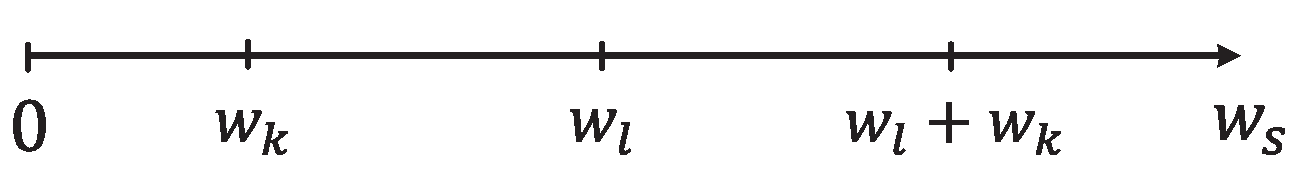
\includegraphics[width=0.7\textwidth]{Chapter3/line.pdf}
\caption{Возможные значения $w_s$}
\label{fig:line}
\end{center}
\end{figure}

Для каждого перечисленного выше интервала построим граничные значения целевой функции (\ref{eq:inter_proof_fksp_lemma_upd}).

\textbf{\textit{Интервал $I$}:}

Построим граничные значения для целевой функции оптимизационной задачи (\ref{eq:inter_proof_fksp_lemma_upd}), при $w_s \in (0, w_k]$. Для этого необходимо соблюсти все ограничения оптимизационной задачи. Важным ограничением является $y_k^{*},y_l^{*} \in [0,1]$. Для обеспечения $y_k^{*} \geq 0$ необходимо, чтобы значение $y_l^{*}$ не превышало $\frac{w_s}{w_l}$. Ограниченность значения $w_s$ величиной $w_k$ приводит невозможности превышения значениями $y_l^{*}$ и $y_k^{*}$ единицы.

Основываясь на данных рассуждениях, $y_l^{*}$ может принимать значения на отрезке $\left[0, \frac{w_s}{w_l}\right]$, и граничные значения могут быть представлены следующим образом:
\begin{itemize}
	\item Граничное значение \textit{$I$.1}:
		$$\begin{cases}
		y_k^{*} = \frac{w_s}{w_k}\\
		y_l^{*} = 0
		\end{cases}.$$
		Значение целевой функции: $f\left(\frac{w_s}{w_k}\right) + f(0)$;
	\item Граничное значение \textit{$I$.2}:
		$$\begin{cases}
		y_k^{*} = 0\\
		y_l^{*} = \frac{w_s}{w_l}
		\end{cases}.$$
		Значение целевой функции: $f(0) + f\left(\frac{w_s}{w_l}\right)$.
\end{itemize}

На основании фактов что функция $f(x)$ является монотонно возрастающей и $w_k < w_l$ следует, что $f\left(\frac{w_s}{w_k}\right) > f\left(\frac{w_s}{w_l}\right)$, так как $\frac{w_s}{w_k} > \frac{w_s}{w_l}$. Следовательно, граничное значение \textit{$I$.1} максимизирует целевую функцию на интервале $I$.

\textbf{\textit{Интервал $II$}:}

На интервале, когда $w_s \in (w_k, w_l]$ важно ограничить сверху значение $y_k^{*}$ единицей, для этого величина $y_l^{*}$ должна превышать $\frac{w_s - w_k}{w_l}$. В тоже время неотрицательность $y_k^{*}$ обеспечивается ограниченностью сверху $y_l^{*}$ величиной $\frac{w_s}{w_l}$. Так же из $w_s \leq w_l$ следует, что $y_l^{*} \leq 1$.

Основываясь на данных рассуждениях, $y_l^{*}$ может принимать значения на отрезке $\left[\frac{w_s - w_k}{w_l}, \frac{w_s}{w_l}\right]$, и граничные значения могут быть представлены следующим образом:

\begin{itemize}
	\item Граничное значение \textit{$II$.1}:
		$$\begin{cases}
		y_k^{*} = 1 \\
		y_l^{*} = \frac{w_s - w_k}{w_l}
		\end{cases}.$$
		Значение целевой функции: $f(1) + f\left(\frac{w_s - w_k}{w_l}\right)$;
	\item Граничное значение \textit{$II$.2}:
		$$\begin{cases}
		y_k^{*} = 0\\
		y_l^{*} = \frac{w_s}{w_l} \leq 1
		\end{cases}.$$
		Значение целевой функции: $f(0) + f\left(\frac{w_s}{w_l}\right) \leq f(0) + f(1)$.
\end{itemize}

Очевидно, что граничное значение \textit{$II$.1} максимизирует целевую функцию на интервале $II$.

\textbf{\textit{Интервал $III$}:}

На интервале $w_s \in (w_l, w_k+w_l)$ проведя рассуждения, аналогичные представленным ранее, $y_l^{*}$ может принимать значения на отрезке $\left[\frac{w_s - w_k}{w_l}, 1\right]$ для выполнения всех ограничений оптимизационной задачи (\ref{eq:inter_proof_fksp_lemma_upd}). Граничные значения могут быть представлены следующим образом:
\begin{itemize}
	\item Граничное значение \textit{$III$.1}:
		$$\begin{cases}
		y_k^{*} = 1 \\
		y_l^{*} = \frac{w_s - w_k}{w_l}
		\end{cases}.$$
		Значение целевой функции: $f(1) + f\left(\frac{w_s - w_k}{w_l}\right)$;
	\item Граничное значение \textit{$III$.2}:
		$$\begin{cases}
		y_k^{*} = \frac{w_s - w_l}{w_k}\\
		y_l^{*} = 1
		\end{cases}.$$
		Значение целевой функции: $f\left(\frac{w_s - w_l}{w_l}\right) + f(1)$.
\end{itemize}

Не составляет трудностей показать, что $\frac{w_s - w_k}{w_l} > \frac{w_s - w_l}{w_k}$, основываясь на следующих неравенствах: $w_s < w_k + w_l$ и $w_k < w_l$. Следовательно, граничное значение \textit{$III$.1} максимизирует целевую функцию на интервале $III$.

Исходя из описанного выше, решение оптимизационной задачи (\ref{eq:inter_proof_fksp_lemma}) задается таблицей \ref{tab:inter_proof_fksp_lemma_solution}. Таблица \ref{tab:inter_proof_fksp_lemma_solution} организована следующим образом: по заданному значению $w_s$ определяются оптимальные значения $y_k^{*}$ и $y_l^{*}$.

\begin{table}[!h]
    \caption{Решение промежуточной оптимизационной задачи}
    \begin{center}
		\label{tab:inter_proof_fksp_lemma_solution}
	    \begin{tabular}{| C{4cm} | C{4cm} | C{4cm} |}
	    	\hline
	    	Значение $w_s$ & Оптимальное значение $y_k^{*}$  & Оптимальное значение $y_l^{*}$ \\
	    	\hline
			$(0, w_k]$ & $$\frac{w_s}{w_k}$$ & $$0$$\\
	    	\hline
			$(w_k, w_k+w_l]$ & $$1$$ & $$\frac{w_s - w_k}{w_l}$$\\
	    	\hline
    	\end{tabular}
	\end{center}
\end{table}

Обобщая изложенное, при всех возможных значениях $w_s$ перераспределение долей взятых предметов в пользу предмета $k$ за счет всей взятой доли предмета $l$ приводит к максимизации целевой функции оптимизационной задачи (\ref{eq:inter_proof_fksp_lemma}) (таблица \ref{tab:inter_proof_fksp_lemma_solution}). Следствием данного факта является, что решение $Y$, возможно улучшить за счет перераспределения долей предметов под индексами $k$ и $l$. Вид решений $X$, $Y$ и $Y^{*}$ представлен на рисунке \ref{fig:X_Y_Ys_Solutions}.

\begin{figure}[htbp]
\begin{center}
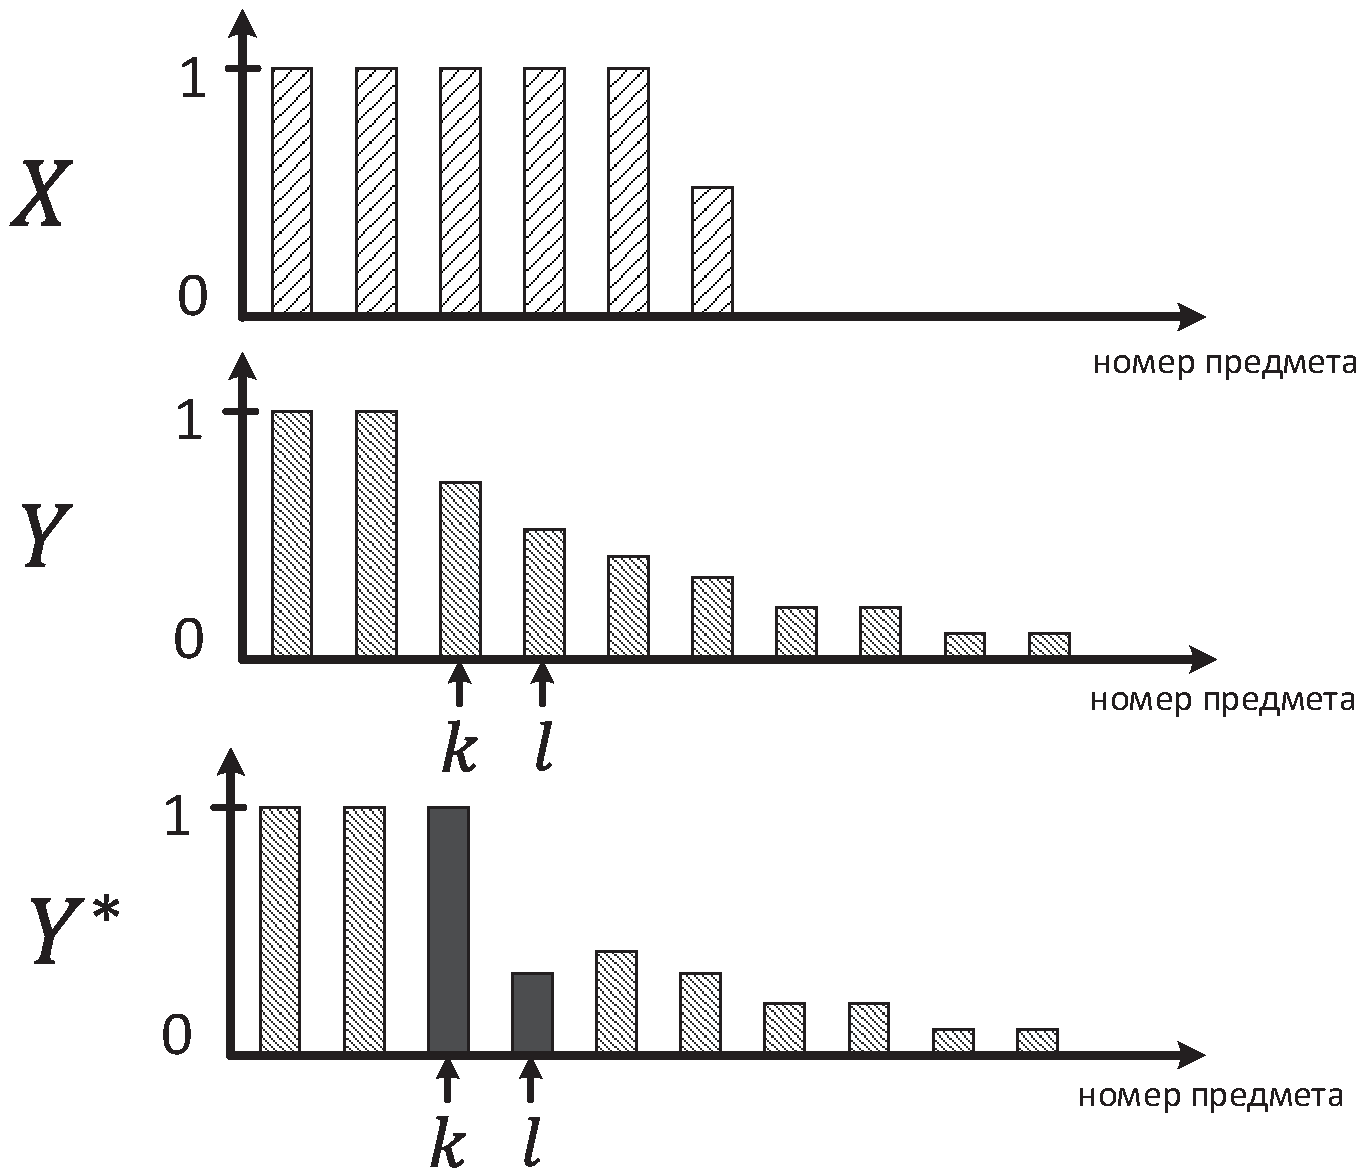
\includegraphics[width=0.6\textwidth]{Chapter3/X_Y_Z.pdf}
\caption{Вид решений $X$, $Y$ и $Y^{*}$}
\label{fig:X_Y_Ys_Solutions}
\end{center}
\end{figure}

Таким образом, любое решение $Y$, в котором найдутся предметы с индексами $k$ и $l$ может быть улучшено до решения $Y^{*}$, значение целевой функции которой больше, чем у $Y$. Большее значение целевой функции при решении $Y^{*}$, по сравнению с $Y$, обеспечивается тем, что $Y^{*}$ является решением промежуточной оптимизационной задачи (\ref{eq:inter_proof_fksp_lemma}).

Следовательно, всевозможные решения $Y$ не являются оптимальными для обобщенной задачи о непрерывном рюкзаке (\ref{eq:fksp_general}), что является противоречием. Одновременно с этим важно отметить, что для решения $X$, полученного по средствам алгоритма \ref{alg:algorithm_lemma}, не найдется пары предметов с индексами $k$ и $l$, следовательно оно не может быть улучшено и является оптимальным для оптимизационной задачи (\ref{eq:fksp_general}).
\end{proof}

Проведем анализ сложности предложенного решения задачи о непрерывном рюкзаке. Для этого рассмотрим каждый шаг алгоритма \ref{alg:algorithm_lemma}:
\begin{itemize}
	\item Шаг 1. Сортировка пользователей в порядке возрастания отношений $\frac{w_i}{c_i}$. Сложность данного шага составляет $O(N \log_2 N), N\to\infty$ при использовании быстрой сортировки;
	\item Шаг 2. Поиск предмета с индексом $j$ может быть осуществлен с линейной сложностью: $O(N), N\to\infty$;
	\item Шаг 3. Вычисление оптимальных значений $x_i, i=\overline{1,N}$ может быть реализовано с линейной сложностью: $O(N), N\to\infty$.
\end{itemize}
В терминах <<$O$>> большого сложность алгоритма в целом определяется самым сложным шагом. Следовательно, сложность алгоритма \ref{alg:algorithm_lemma} определяется Шагом 1 и равняется $O(N \log_2 N), N\to\infty$.

Для непрерывных задач выпуклого программирования от нескольких переменных с ограничениями типа равенств и неравенств существуют несколько способов отыскания экстремумов \cite{convex_opt,optimizations_methods}:
\begin{itemize}
	\item Получение замкнутого выражения на основе условий Каруша-Куна-Таккера (ККТ);
	\item Получение численного решения на основе условий ККТ;
	\item Численные методы нелинейного программирования.
\end{itemize}

Стандартным методом решения задач выпуклого программирования является поиск решения удовлетворяющих условиям Каруша-Куна-Таккера \cite{convex_opt,optimizations_methods}. Данный метод сводится к нахождению решения системы нелинейных уравнений и неравенств. В результате решения данной системы может быть получено замкнутое выражение для условного экстремума. Тогда сложность полученного решения заключается в вычислении значений по заданным входным данным. Сложность вычисления решения растет линейно от числа переменных $N$: $O(N), N\to\infty$.

Однако, ввиду большого числа переменных в системе, полученной на основе условий ККТ, получение замкнутого решения может быть затруднительно. Для решения подобных систем может быть применен метод, известный в англоязычной литературе как \textit{<<water-filling>>}, подробно описанный в \cite{convex_opt}. Данный метод позволяет найти решение системы, которое может быть полученно с использованием численной процедуры. В настоящей работе, метод \textit{<<water-filling>>} был применен для решения оптимизационной задачи, представленной в подразделе \ref{chap4:KktSolution}. Сложность вычисления решения определяется сложностью процедуры получения численного решения.

Для решения задач выпуклого программирования от нескольких переменных с ограничениями типа равенств и неравенств известны численные методы решения: методы спуска и штрафных функций \cite{optimizations_methods}. Важно отметить, что для задач выпуклого программирования данные методы сходятся к оптимальному решению, так как в подобных задачах существует только один экстремум. Оценить сложность получения решения оптимизационных задач с использованием подобных методов не представляется возможным, так как данные методы являются итеративными и зависят от начальных значений поиска экстремума (невозможно предсказать количество шагов, необходимых для нахождения оптимальных значений оптимизационной задачи). Сравнение сложности методов решения оптимизационных задач выпуклого программирования от нескольких переменных с ограничениями типа равенств и неравенств представлены в таблице~\ref{tab:nonadaptiveComplexity}.

\begin{table}[!h]
    \caption{Сравнение сложности методов решения обобщенной задачи о непрерывном рюкзаке}
    \begin{center}
		\label{tab:nonadaptiveComplexity}
	    \begin{tabular}{| C{5cm} | C{5cm} | C{5cm} |}
	    	\hline
	    	Название метода & Характеристика сложности метода при наличии $N$ переменных & Возможность реализации в реальном масштабе времени\\
	    	\hline
			Замкнутое выражение (ККТ) & $$O(N), N\to\infty$$ & $$+$$\\
	    	\hline
			Решение на основе алгоритма \ref{alg:algorithm_lemma} & $$O(N \log_2 N), N\to\infty$$ & $$+$$\\
	    	\hline
	    	Численное решение системы условий ККТ & Зависит от процедуры получения численного решения & $$+/-$$ \\
	    	\hline
	    	Численные методы нелинейного программирования & Высокая сложность & $$-$$ \\
	    	\hline
    	\end{tabular}
	\end{center}
\end{table}

Таким образом, при сравнении сложности полученного решения на основе алгоритма \ref{alg:algorithm_lemma} со стандартными методами решения непрерывных задач выпуклого программирования от нескольких переменных с ограничениями типа равенств и неравенств справедливо следующее утверждение. Сложность решения на основе алгоритма \ref{alg:algorithm_lemma} является приемлемой в сравнении со стандартными методами решения подобных задач.

В дополнении сказанного выше, решение оптимизационной задачи (\ref{eq:fksp_general}) алгоритмом \ref{alg:algorithm_lemma} может быть вычислено в режиме реального времени. Под режимом реального времени понимается возможность вычисления оптимальных значений в короткий промежуток времени. В настоящей работе за единицу времени принят интервал планирования равный $1$ мс (подраздел~\ref{chap2:RadioChannel}). Элементарно показывается, что на современных процессорах алгоритм \ref{alg:algorithm_lemma} может быть выполнен за промежуток времени не превышающий интервал планирования.

\section{Нижняя граница нормированного отношения длительности буферизации к просмотру при передаче неадаптивных видеопотоков}
\label{chap3:LowerBoundForG}

В подразделе \ref{chap3:NonAdaptiveOptimizationProblem} была поставлена оптимизационная задача нелинейного программирования (\ref{eq:optim_problem_g}), на основе решения которой возможно найти нижнюю границу для средне-пользовательского значения нормированного отношения длительности ожидания к просмотру: $G$ (определение~\ref{def:gMetric}) по всевозможным алгоритмам планирования $\mathcal{A}(\cdot)$, удовлетворяющих введенных ограничениям в подразделе \ref{chap2:Assumptions}. В подразделе \ref{chap3:GeneralizedFKSP} была представлена обобщенная задача о непрерывном рюкзаке, когда в целевой функции фигурирует сумма выпуклых функций, и предложен алгоритм нахождения решения данной задачи, с низкой вычислительной сложностью. Настоящий подраздел ставит своей задачей основываясь на результатах, полученных в подразделе \ref{chap3:GeneralizedFKSP}, найти нижнюю границу для критерия качества $G$.

Оптимизационная задача (\ref{eq:optim_problem_g}) имеет следующий вид:
\begin{equation}
\nonumber
\begin{array}{l}
\text{ \textbf{Минимизировать:} } G = \sum\limits_{i=1}^{N} {g_i} \\
\text{ \textbf{При условии:} }\\
\begin{cases}
\sum\limits_{i=1}^{N} {\frac{K_i (1-g_i)}{g_i + \gamma (1-g_i)}} \leq 1 \\
g_i \in [0,1], i=\overline{1,N}
\end{cases}
\end{array},
\end{equation}
где $K_i=R_i E[C_i^{-1}]$, $\gamma$~--~коэффициент разряженности видеопотока (определение \ref{def:VideoSparseness}).

\begin{theoremapp}
\label{thr:GTheorem}
Решение задачи нелинейного программирования (\ref{eq:optim_problem_g}), характеризующее нижнюю границу нормированного отношения длительности буферизации к просмотру при передаче неадаптивных видеопотоков, может быть получено по средствам алгоритма \ref{alg:GTheoremAlgorithm}.
\end{theoremapp}

\begin{algorithm}
  \caption{: Решение задачи (\ref{eq:optim_problem_g})}
	\label{alg:GTheoremAlgorithm}
  \begin{algorithmic}[1]
	 \item Сортировка пользователей по возрастанию отношений $\frac{K_i}{\gamma}$, и их нумерация, в соответствие с сортировкой;
	 \item Нахождение пользователя с индексом $j:\begin{cases}
		\sum\limits_{i=1}^{j-1} {\frac{K_i}{\gamma}} \leq 1 \\
		\sum\limits_{i=1}^{j} {\frac{K_i}{\gamma}} > 1
		\end{cases}$
		\newline
		если $j\in\varnothing, j=N+1$;
	\item Нахождение оптимальных значений $g_i$: \newline
	$g_i=\begin{cases}
		0, & i < j \\
		\frac{\gamma (1 - \xi)}{\xi + \gamma (1-\xi)}, & i=j \\
		1, & i > j
		\end{cases}$,\newline
		где $\xi = \frac{\gamma}{K_j}\left(1 - \sum\limits_{i=1}^{j-1} {\frac{K_i}{\gamma}}\right)$.
  \end{algorithmic}
\end{algorithm}

\begin{proof}

Для доказательства теоремы \ref{thr:GTheorem} произведем несколько преобразований системы (\ref{eq:optim_problem_g}).

Изначально вынесем из знаменателя нелинейного ограничения $\gamma$:

$$\sum\limits_{i=1}^{N} {\frac{K_i (1-g_i)}{g_i + \gamma (1-g_i)}} = \sum\limits_{i=1}^{N} \left(\frac{K_i}{\gamma}\right) {\frac{(1-g_i)}{\frac{g_i}{\gamma} + (1-g_i)}}.$$

Далее произведем преобразование задачи (\ref{eq:optim_problem_g}) из задачи минимизации в задачу максимизации:

\begin{equation}
\nonumber
\label{eq:GTheorem_1}
\begin{array}{l}
\text{ \textbf{Максимизировать:} } \sum\limits_{i=1}^{N} {(1-g_i)} \\
\text{ \textbf{При условии:} }\\
\begin{cases}
\sum\limits_{i=1}^{N} \left(\frac{K_i}{\gamma}\right) {\frac{(1-g_i)}{\frac{g_i}{\gamma} + (1-g_i)}} \leq 1 \\
g_i \in [0,1], i=\overline{1,N}
\end{cases}
\end{array}.
\end{equation}

Введем обозначение:
$$x_i = \frac{(1-g_i)}{\frac{g_i}{\gamma} + (1-g_i)}.$$
Важно отметить, что значение $x_i$ монотонно зависит от величины $g_i$ и может принимать значения в отрезке $[0,1]$. Выразим значения $g_i$ и $(1-g_i)$ из $x_i$:
\begin{equation}
\label{eq:GTheorem_interrelation}
g_i = \frac{\gamma (1 - x_i)}{x_i + \gamma (1-x_i)}.
\end{equation}
$$1-g_i = \frac{x_i}{x_i + \gamma (1-x_i)}.$$

Основываясь на введенных обозначениях, оптимизационная задача (\ref{eq:optim_problem_g}) принимает следующий вид:
\begin{equation}
\label{eq:GTheorem_2}
\begin{array}{l}
\text{ \textbf{Максимизировать:} } \sum\limits_{i=1}^{N} {\frac{x_i}{x_i + \gamma (1-x_i)}} \\
\text{ \textbf{При условии:} }\\
\begin{cases}
\sum\limits_{i=1}^{N} \left(\frac{K_i}{\gamma}\right) {x_i} \leq 1 \\
x_i \in [0,1], i=\overline{1,N}
\end{cases}
\end{array}.
\end{equation}

Проведем анализ целевой функции оптимизационной задачи (\ref{eq:GTheorem_2}) и покажем, что данная целевая функция соответствует требованиям, налагаемыми на целевую функцию оптимизационной задачи (\ref{eq:fksp_general}). Из вида функции очевидно, что она непрерывна, строго монотонно возрастает и ограниченна сверху и снизу на области определения $x_i$. Проведем анализ второй производной:
$$\left[\frac{x_i}{x_i + \gamma (1-x_i)}\right]'' = \frac{2\gamma(\gamma - 1)}{(x_i + \gamma(1 - x_i))^3}.$$
По определению, значение $\gamma \geq 1$, так же величина $x_i$, по условию оптимизационной задачи, может принимать значения в отрезке $[0,1]$, следовательно вторая производная неотрицательна в области определения $x_i$.

Основываясь на представленном анализе, $\frac{x_i}{x_i + \gamma (1-x_i)}$~--~непрерывная, выпуклая вниз функция, дважды дифференцируемая, строго монотонно возрастающая и ограниченная на области определения $x_i$ функция. Исходя и описанного выше и результатов, представленных в подразделе \ref{chap3:GeneralizedFKSP}, справедливо следующее утверждение: решение задачи (\ref{eq:GTheorem_2}) может быть получено при использовании алгоритма \ref{alg:algorithm_lemma}, где $w_i = \left(\frac{K_i}{\gamma}\right), c_i = 1, i=\overline{1,N}$ и $W = 1$.

Алгоритм \ref{alg:GTheoremAlgorithm} является адаптацией алгоритма \ref{alg:algorithm_lemma} в обозначениях оптимизационной задачи (\ref{eq:optim_problem_g}) и взаимосвязи между значениями $g_i$ и $x_i$ (\ref{eq:GTheorem_interrelation}). Данный факт завершает доказательство.
\end{proof}

Результатом решения задачи (\ref{eq:optim_problem_g}) является вектор отношений длительности буферизации к просмотру для каждого пользователя: $(g_1, g_2, \ldots, g_N)$, обладающий минимально возможной суммой элементов, удовлетворяющих всем ограничениям оптимизационной задачи. Среднее арифметическое элементов данного вектора является нижней границей по всем возможным алгоритмам планирования распределения ресурсам, удовлетворяющим допущениям, введенным в подразделе \ref{chap2:Assumptions}. Обобщая сказанное ранее, в настоящем разделе была найдена граница, характеризующая максимально возможную производительность алгоритмов распределения ресурсов радиоканала в централизованных беспроводных телекоммуникационных сетях при передачи неадаптивных видеопотоков.

Настоящий результат имеет широкий спектр применения:
\begin{itemize}
	\item \textbf{Теоретическая область.} Нижняя граница может быть использована для аналитической оценки производительности централизованных беспроводных для существующих и последующих стандартов беспроводной связи.
	\item \textbf{Практическая область.} Благодаря невысокой вычислительной сложности вычисления нижней границы (алгоритм \ref{alg:GTheoremAlgorithm}), настоящая нижняя граница может быть непосредственно встроена в алгоритм распределения ресурсов беспроводного канала на базовой станции. Такая возможность позволяется создать семейство алгоритмов планирования для повышения производительности сети передачи информации в целом.
\end{itemize}

Завершающая часть настоящего раздела посвящена демонстрации области практической применимости полученного результата. Далее в разделе будет предложен алгоритм планирования ресурсов беспроводного канала на базовой станции и произведено его сравнение с известными планировщиками и нижней границей.

\section{Алгоритм планирования распределения ресурсов для нормированного отношения длительности буферизации к просмотру при передаче неадаптивных видеопотоков}
\label{chap3:NonAdaptiveScheduler}

Настоящий подраздел описывает концепцию алгоритма планирования распределения ресурсов на базовой станции, в основу которого положен результат, представленный в подразделе \ref{chap3:LowerBoundForG}. В настоящем подразделе будет предложен планировщик, опирающийся на концепцию совместного планирования ресурсов радиоканала между всеми активными пользователями, в отличии от классических алгоритмов планирования (подраздел \ref{chap2:Scheduler}). Под совместным планированием подразумевается учет при распределении частотно-временных ресурсов конкретному пользователю не только его статистики, но и статистик всех активных пользователей, присутствующих в системе передачи информации в момент планирования.

Настоящий подраздел последовательно описывает этапы построения алгоритма планирования:
\begin{itemize}
	\item Определение объема доступной информации для принятия решения;
	\item Статистики и методы их вычисления;
	\item Методы управления распределением частотно-временных ресурсов;
	\item Алгоритм распределения ресурсов беспроводного канала.
\end{itemize}

В начале будет представлено общее описание рассматриваемой системы. На рисунке~\ref{fig:PracticalModel} представлена концептуальная схема беспроводной централизованной сети при передаче видеоданных, основанная на описании представленному в подразделах \ref{chap2:GeneralOverview}, \ref{chap2:RadioChannel} и \ref{chap2:Scheduler}. Важным функциональным компонентом опорной сети оператора в современных стандартах связи является система анализа трафика, которая может определить тип используемого трафика и его характеристики (в англоязычной литературе данные системы известны под названием \textit{<<Deep Packet Inspection>>} или DPI). Центральным элементом рассматриваемой схемы является планировщик базовой станции. Важным моментом в настоящем описании является объемы и моменты времени доступа к информации на основе которой алгоритм планировщика будет принимать решения распределении ресурсов беспроводного канала.

\begin{figure}[htbp]
\begin{center}
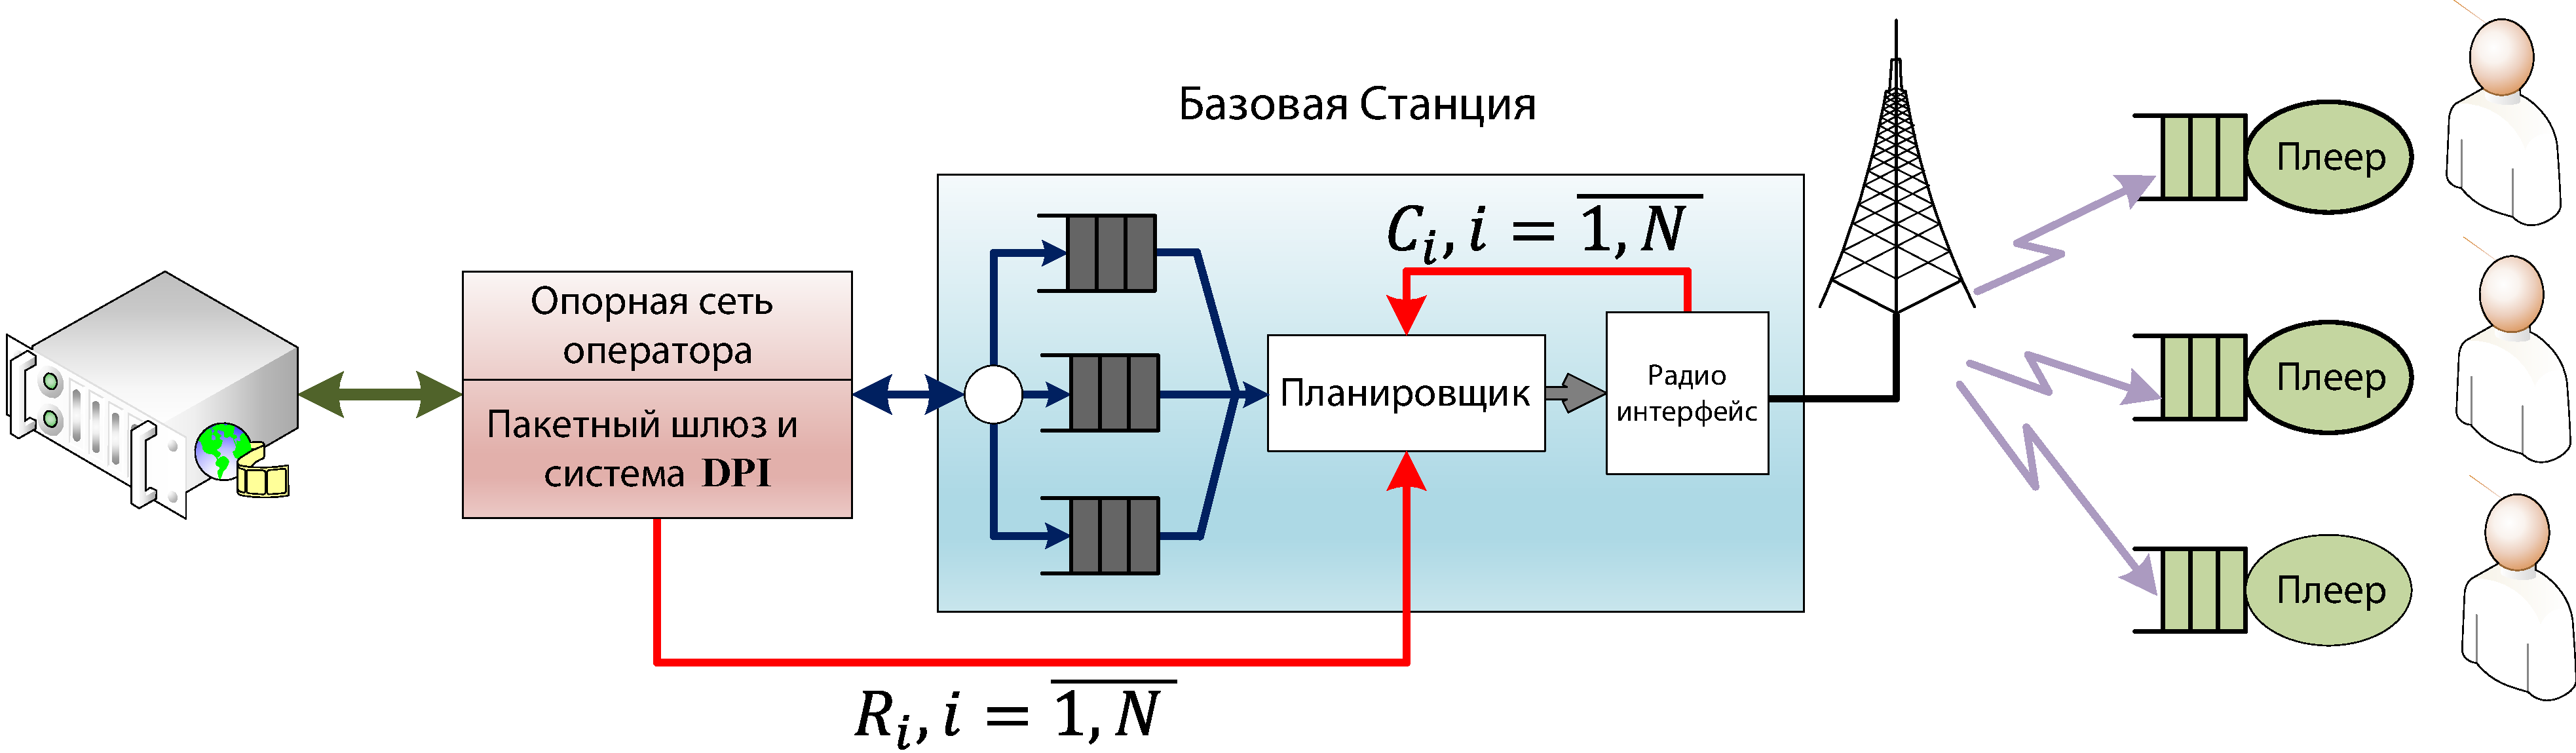
\includegraphics[width=\textwidth]{Chapter3/PracticalModel.pdf}
\caption{Концептуальная схема предлагаемого алгоритма планирования}
\label{fig:PracticalModel}
\end{center}
\end{figure}

На первом шаге описания алгоритма планирования будет представлена информация, доступная алгоритму планирования, для принятия решения. В настоящей работе, для планировщика доступна следующая информация для каждого пользователя $i$ в каждый момент времени $t$:
\begin{itemize}
	\item Битовая скорость потока $R_i(t)$, полученная от системы анализа трафика DPI;
	\item Значение максимально достижимой скорости канала $C_i(t)$, значение которой доступно от радио интерфейса;
	\item Объем данных доступный в очереди для передачи на пользовательское устройство $B_i(t)$;
	\item Объем переданных данных $P_i(t)$.
\end{itemize}
Важно отметить, что в существующих беспроводных централизованных системах связи время является дискретным и разбито на интервалы равной длительности $\Delta t$ секунд.

На втором шаге описания алгоритма предлагаются методы агрегирования доступной информации. Представленный ранее объем информации должен быть агрегирован в некоторые значения, называемые статистиками, которые отражают текущую ситуацию в зоне ответственности базовой станции. Наиболее критичные статистики, необходимые для функционирования планировщика, представлены следующим списком:
\begin{itemize}
	\item Активность пользователя $U_i(t)$;
	\item Оценка скорости передачи информации $S_i^{avg}(t)$;
	\item Оценка максимально достижимой скорости канала $C_i^{avg}(t)$.
\end{itemize}
Сложность вычисления данных статистик является важным ограничением, налагаемым на вычислительную процедуру, ввиду жесткого временного ограничения на длительность получения результата (подраздел \ref{chap2:Scheduler}).

В настоящей работе рассматривается модель поведения пользователя, просматривающего последовательность роликов (подраздел \ref{chap2:GeneralOverview}). Следовательно, пользователь может находится в двух состояниях: активном (загружает видеоданные) или неактивном (выбирает следующий ролик для просмотра). Таким образом, на уровне планировщика необходимо произвести оценку $U_i(t)$: в каком из двух состояний находится пользователь $i$ в момент времени $t$. Активность пользователя определяется логическим значением (истинно или ложно). Будем считать пользователя активным, если разность между текущим моментом времени и последним моментом времени, когда у абонента $i$ были данные для передачи не превышает $t^{act}$ секунд:
\begin{equation}
	\label{eq:activityEstimation}
	U_i(t) = \mathbbm{1}\{t - t_i^{l} \leq t^{act}\},
\end{equation}
где $t_i^{l} = \max\limits_{t} \mathbbm{1}\{B_i(t) > 0\}.$

Для прощения последующего повествования введем обозначение $\mathcal{U}$~--~множество активных пользователей ($i:U_i(t) > 0$) в момент времени $t$. 

Так как в настоящей работе рассматривается передача информации по беспроводному каналу связи, важной отличительной чертой которого является изменяемость характеристик во времени (подраздел \ref{chap2:RadioChannel}). В качестве статистики для оценок $S_i^{avg}(t)$ и $C_i^{avg}(t)$ в настоящей работе предлагается использовать среднее значение за продолжительный промежуток времени (длительность усреднения) $\bar{w}_{S}$ и $\bar{w}_{C}$ соответственно. Ограничение интервала усреднения обусловлены изменяемостью канала связи и необходимостью поддержания актуальности статистик.

Простейшим подходом для вычисления средних значений является среднее арифметическое значение, однако, сложность его вычисления по операциям и затрачиваемым объемом памяти достаточно высока: хранение всего массива исходных данных и его обработка. Ввиду существующих ограничений на сложность в качестве метода оценки предлагается использовать метод экспоненциального забывания (в литературе встречается термин <<экспоненциальное сглаживание>>):

$$X_i^{avg}(t) = \left(1 - \frac{1}{\bar{w}_{X}}\right)X_i^{avg}(t - 1) + \left(\frac{1}{\bar{w}_{X}}\right)X_i(t),$$
где $X_i(t)$~--~элемент дискретного случайного процесса, $\bar{w}_{X}$~--~длительность усреднения для процесса $X$ и $X_i^{avg}(0) = X_i(1)$.

Важной характеристикой методов оценки среднего значения за некоторый промежуток времени является скорость сходимости полученной оценки к истинному значению. На скорость сходимости среднего значения, вычисленного методом экспоненциального забывания, к истинному значению большое влияние оказывает длительности интервалов усреднения. Во многих случаях оценка среднего значения методом среднего арифметического и экспоненциального забывания показывает близкие значения. Однако, существует сценарий, на котором оценки, полученные по настоящим методикам, показывают разную скорость сходимости к истинному среднему значению. Подобная ситуация возможна, когда первое значение случайного процесса имеет сильное отличие от истинного среднего. Продемонстрируем это на примере: пусть существует дискретный случайный процесс $X(t) \sim N(10,1.5)$, при этом значение $X(1) = 0$, и необходимо произвести оценку его среднего значения за последние $\bar{w}_{X} = 10$ отсчетов (рисунок \ref{fig:adaptation}).

Из рисунка \ref{fig:adaptation} следует, что метод экспоненциального ожидания при оценке среднего значения показывает медленную скорость сходимости к истинному среднему значению по сравнению с методом среднего арифметического. Поэтому в настоящем подразделе предлагается модифицировать метод экспоненциального забывания изменяемым во времени интервалом усреднения по следующему правилу:
$$w_{X}(t) = \min(t, \bar{w}_{X}).$$
В настоящей работе, метод оценки среднего значения, использующий изменяемый во времени интервал усреднения называется \textit{<<методом экспоненциального забывания с быстрой адаптацией>>}. Производительность данного метода оценки сравнима с методом среднего арифметического и демонстрирует достаточную скорость сходимости к истинному значению (рисунок \ref{fig:adaptation}).

\begin{figure}[htbp]
\begin{center}
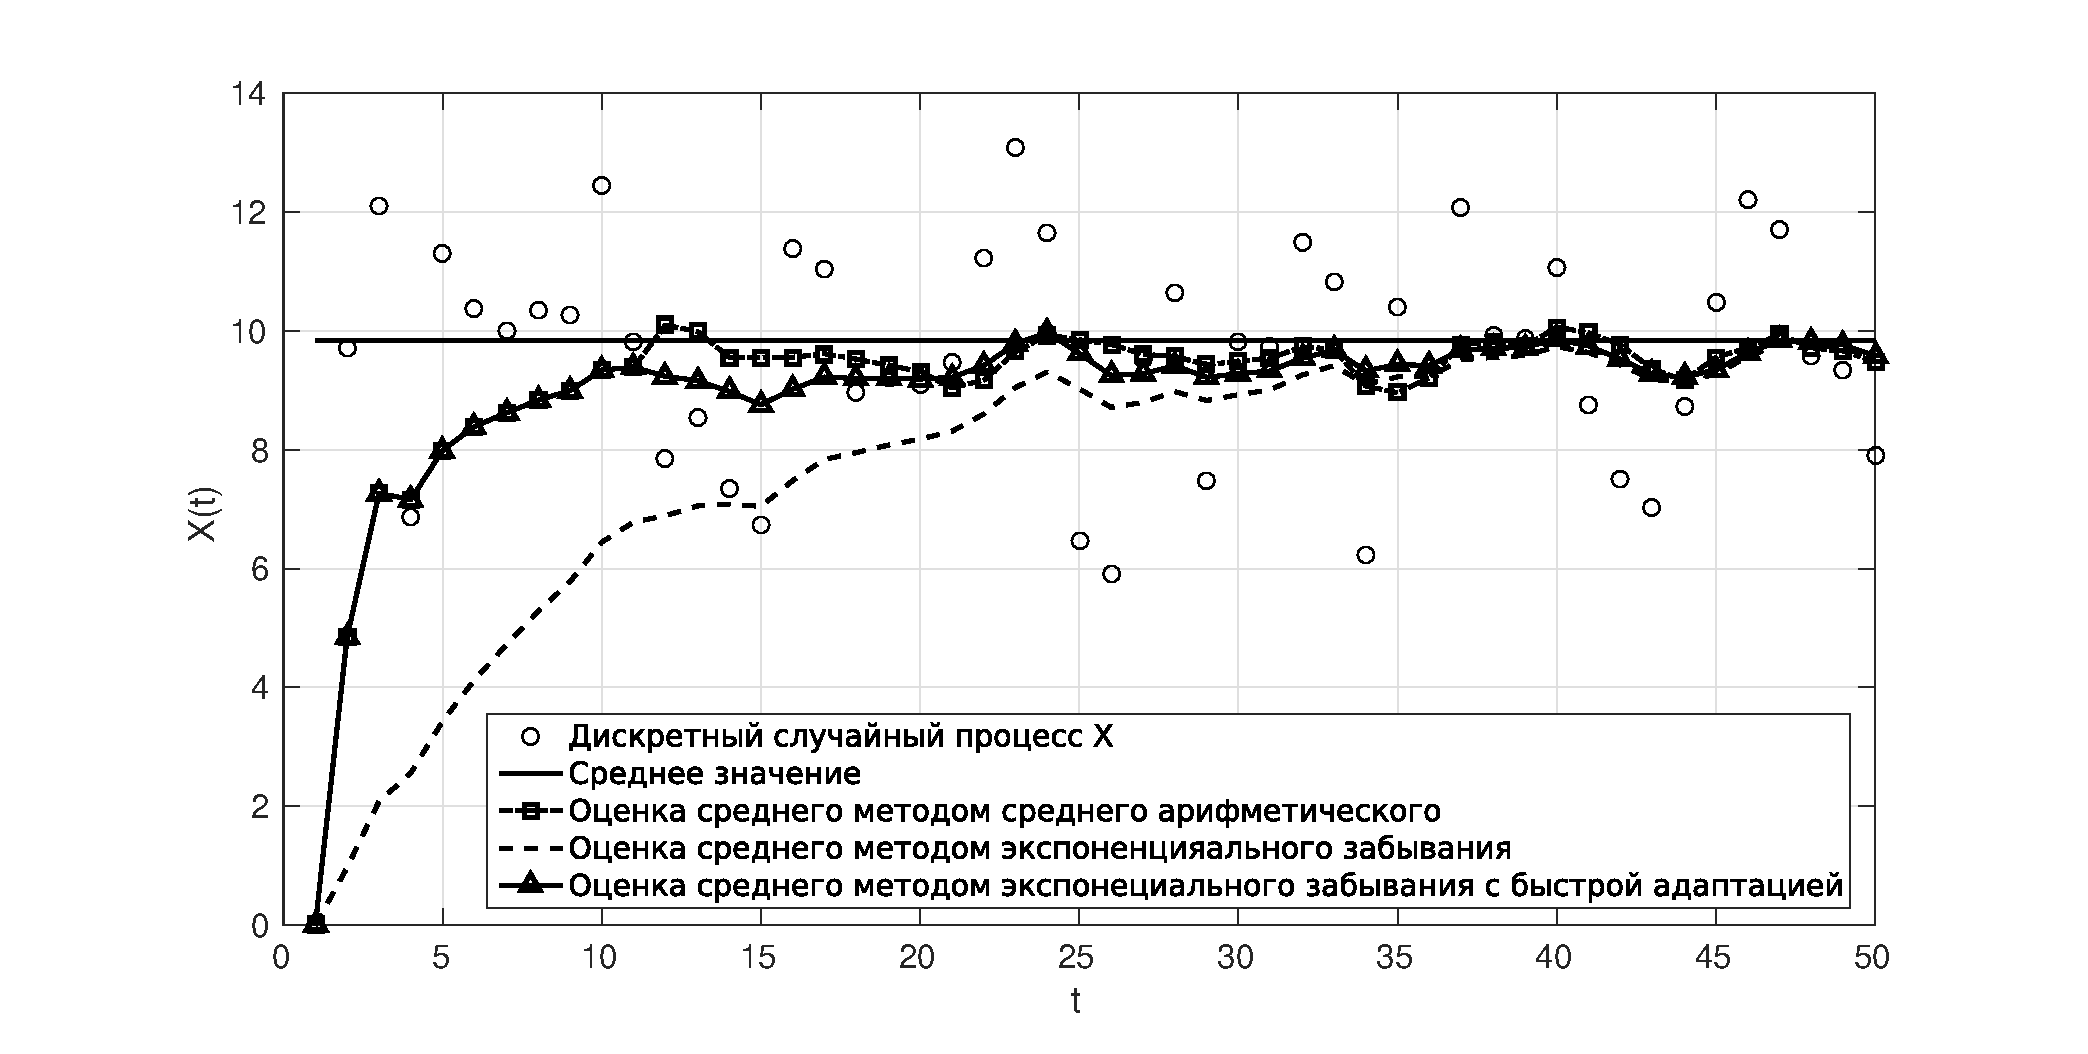
\includegraphics[width=\textwidth]{Chapter3/adaptation.eps}
\caption{Сравнение скорости сходимости методов оценки среднего значения}
\label{fig:adaptation}
\end{center}
\end{figure}

Обобщая сказанное выше, для оценки оценки средних значений $C_i^{avg}(t)$ и $S_i^{avg}(t)$ предлагаются следущие методики, вычисление которых производится только в активном состоянии пользователя:
\begin{equation}
\label{eq:CEstimation}
C_i^{avg}(t) = \left(1 - \frac{1}{w_{C}(t)}\right)C_i^{avg}(t - 1) + \left(\frac{1}{w_{C}(t)}\right)C_i(t)
\end{equation}

\begin{equation}
\label{eq:SEstimation}
S_i^{avg}(t) = \left(1 - \frac{1}{w_{S}(t)}\right)S_i^{avg}(t - 1) + \left(\frac{1}{w_{S}(t)}\right)\frac{P_i(t)}{\Delta t},\end{equation}
где $w_{C}(t) = \min (t - t_i^{l} + 1, \bar{w}_{C})$ и $w_{S}(t) = \min (t - t_i^{l} + 1, \bar{w}_{S})$  соответственно и $C_i^{avg}(0) = S_i^{avg}(0) = 0$.

Неотрицательность значений $w_{C}(t)$ и $w_{S}(t)$ обеспечиваются вычислением оценок только в активном состоянии пользователя ($t - t_i^{l} \geq 0$). Подобный метод оценки поддерживает актуальность статистик, так как канал может динамично меняться во времени, а так же обладает низкой вычислительной сложностью.

Следующим шагом в представлении алгоритма планирования является метод управления распределением частотно-временных ресурсов, имеющего непосредственное влияние на скорость передачи информации. Для представления данного метода необходимо представить описание каким образом существующие алгоритмы планирования распределяют ресурсы беспроводного канала связя. Как было описано в подразделе \ref{chap2:RadioChannel}, беспроводной канал связи разделен на ресурсные блоки, являющиеся минимальной единицей ресурсов, которая может быть выделена пользователю. Количество ресурсных ($N_{rb}$) блоков в одном интервале планирования определяется шириной полосы.

В каждый момент времени $t$ для конкретного ресурсного блока $r$ вычисляется приоритет выделения для каждого пользователя $i$: $p_{r,i}(t)$, по некоторому правилу. Далее, для каждого конкретного ресурсного блока находится пользователь с максимальным приоритетом и выделяется найденному пользователю. Важно отметить, что все алгоритмы планирования не распределяют ресурсы пользователям, у которых ответствуют данные для передачи на Уровне очередей. Именно правило вычисления приоритета пользователя на ресурсный блок определяет алгоритм планирования. Наиболее известными эвристическими алгоритмами планирования являются \textit{Proportional Fair} и \textit{Round Robin}:
\begin{itemize}
	\item \textit{Proportional Fair} ставит своей целевой функцией обеспечение равных скоростей передачи информации:
	$$p^{PF}_{r,i}(t) = \frac{C_i^{avg}(t)}{S_i^{avg}(t)};$$
	\item \textit{Round Robin} обеспечивает равный доступ к ресурсам беспроводного канала за счет цикличного распределения ресурсных блоков между активными пользователями.
\end{itemize}

Важной отличительной чертой классических планировщиков является независимость вычисления приоритета пользователя для конкретного блока ресурсов от других пользователей. В настоящей работе предлагается иная концепция планирования: совместное планирование распределения ресурсов, в котором важную роль выполняет зависимость вычисление приоритета от характеристик всего множества пользователей: их числа, вида трафика, требований к обслуживанию и т.д.

Аналитические исследования производительности систем передачи информации, аналогичные представленным в подразделе \ref{chap3:LowerBoundForG}, позволяют оценить скорость обслуживания для каждого конкретного абонента в зависимости от ситуации в соте. Таким образом, в каждый момент времени может быть вычислена <<рекомендуемая>> скорость передачи информации для максимизации производительности сети в соответствии с некоторым критерием. В свою очередь, рекомендуемая скорость обеспечивает максимальную производительность системы, при условии ее обеспечения. Обобщая сказанное выше, для реализации концепции совместного планирования распределения ресурсов необходимо решить две задачи:
\begin{itemize}
	\item Предложить алгоритм расчета рекомендованной скорости передачи данных, на основе ограниченного объема информации доступного планировщику базовой станции;
	\item Предложить механизм обеспечения рекомендованной скорости передачи данных.
\end{itemize}

Изначально будет предложен механизм обеспечения рекомендуемой скорости передачи информации $S^{rec}_i(t)$ пользователю $i$. Основной функцией алгоритма планирования является выделение абонентам частотно-временных ресурсов: в каждый момент времени планировщик принимает решение о доле выделенных ресурсов для всех пользователей (подраздел \ref{chap2:Scheduler}). На основе данных возможностей, управление скоростью передачи информации на уровне доступа ко среде может быть осуществлено за счет контроля частоты выделения ресурсов. Пусть некоторому абоненту $i$ необходимо обеспечить скорость получения информации $S^{rec}_i(t)$. Алгоритм планирования может оценить скорость передачи информации в каждый момент времени $t$ на основе выражения (\ref{eq:SEstimation}). Для того чтобы скорость получения информации не превышала рекомендованной скорости возможно применить следующий подход: пользователь $i$ участвует в распределении ресурсов в момент $t$, если $\mathbbm{1}\{S_i^{avg}(t) \leq S^{rec}_i(t)\}.$

Выберем в качестве основы алгоритм \textit{Proportional Fair} и произведем его объединение с механизмом ограничения скорости передачи информации:
\begin{equation}
\label{eq:PriorFunction}
p_{r,i}(t) = \mathbbm{1}\{S_i^{avg}(t) \leq S^{rec}_i(t)\}\frac{C_i^{avg}(t)}{S_i^{avg}(t)}.
\end{equation}
Расчет приоритета пользователя на основе выражения (\ref{eq:PriorFunction}) позволяет обеспечить скорость передачи информации не превышающую рекомендованной. Важно отметить, что если в некоторый момент времени у всех активных пользователей оценка скорости превышает рекомендованные, то у них всех будут равные приоритеты на ресурсные блоки, и они могут быть выделены случайным абонентам для полного использования ресурсов беспроводного канала.

После выбора механизма управления скоростью передачи информации необходимо детерминировать алгоритм вычисления рекомендованных скоростей передачи информации, чтобы на их основе организовать управление передачей данных. Предполагается, что на алгоритме планирования для всех пользователей, просматривающих видео, известна оценка битовой скорости видеопотока $\left(\hat{R}_i(t)\right)$, просматриваемого в текущий момент времени, от системы анализа трафика DPI и оценка максимально достижимой скорости канала $\left(C^{avg}_i(t)\right)$, на основе выражения (\ref{eq:CEstimation}). Данный объем информации позволяет произвести вычисление оценки нижней границы нормированного отношения длительности буферизации к просмотру при передаче неадаптивных видеопотоков $\hat{G}(t) = \{\hat{g}_i(t), i \in \mathcal{U}\}$ для всего множества активных пользователей в момент времени $t$, при $K_i = \hat{R_i}(t) / C^{avg}_i(t)$ и $\gamma = 1$, так как планирование производится только для множества активных пользователей.

На основе оценки $\hat{G}(t)$ рекомендованные скорости предлагается вычислять следующим образом:
\begin{equation}
\label{eq:SReqCalc}
S^{rec}_i(t) =
\begin{cases}
\hat{R}_i(t) (1 - \hat{g}_i(t)), & \hat{g}_i(t) \in [0,1) \\
S^{min}, &  \hat{g}_i(t) = 1 \\
0,& i \notin \mathcal{U}
\end{cases}, i = \overline{1,N},
\end{equation}
где $S^{min}$~--~минимальная скорость передачи информации, обеспечиваемая алгоритмом планирования. Значение минимальной скорости обслуживания абонентов определяется стандартами связи.

Соотвественно доли ресурсов беспроводного канала для каждого пользователя $i$ в момент времени $t$ могут быть выражены следующим образом:
$$\alpha_i(t) = \begin{cases}
					\frac{\hat{R_i}(t) (1 - \hat{g}_i(t)) + S^{min}}{C^{avg}_i(t)}, & i \in \mathcal{U}  \\
					0, & i \notin \mathcal{U}
					\end{cases}, i = \overline{1,N}.$$

\begin{figure}[htbp]
\begin{center}
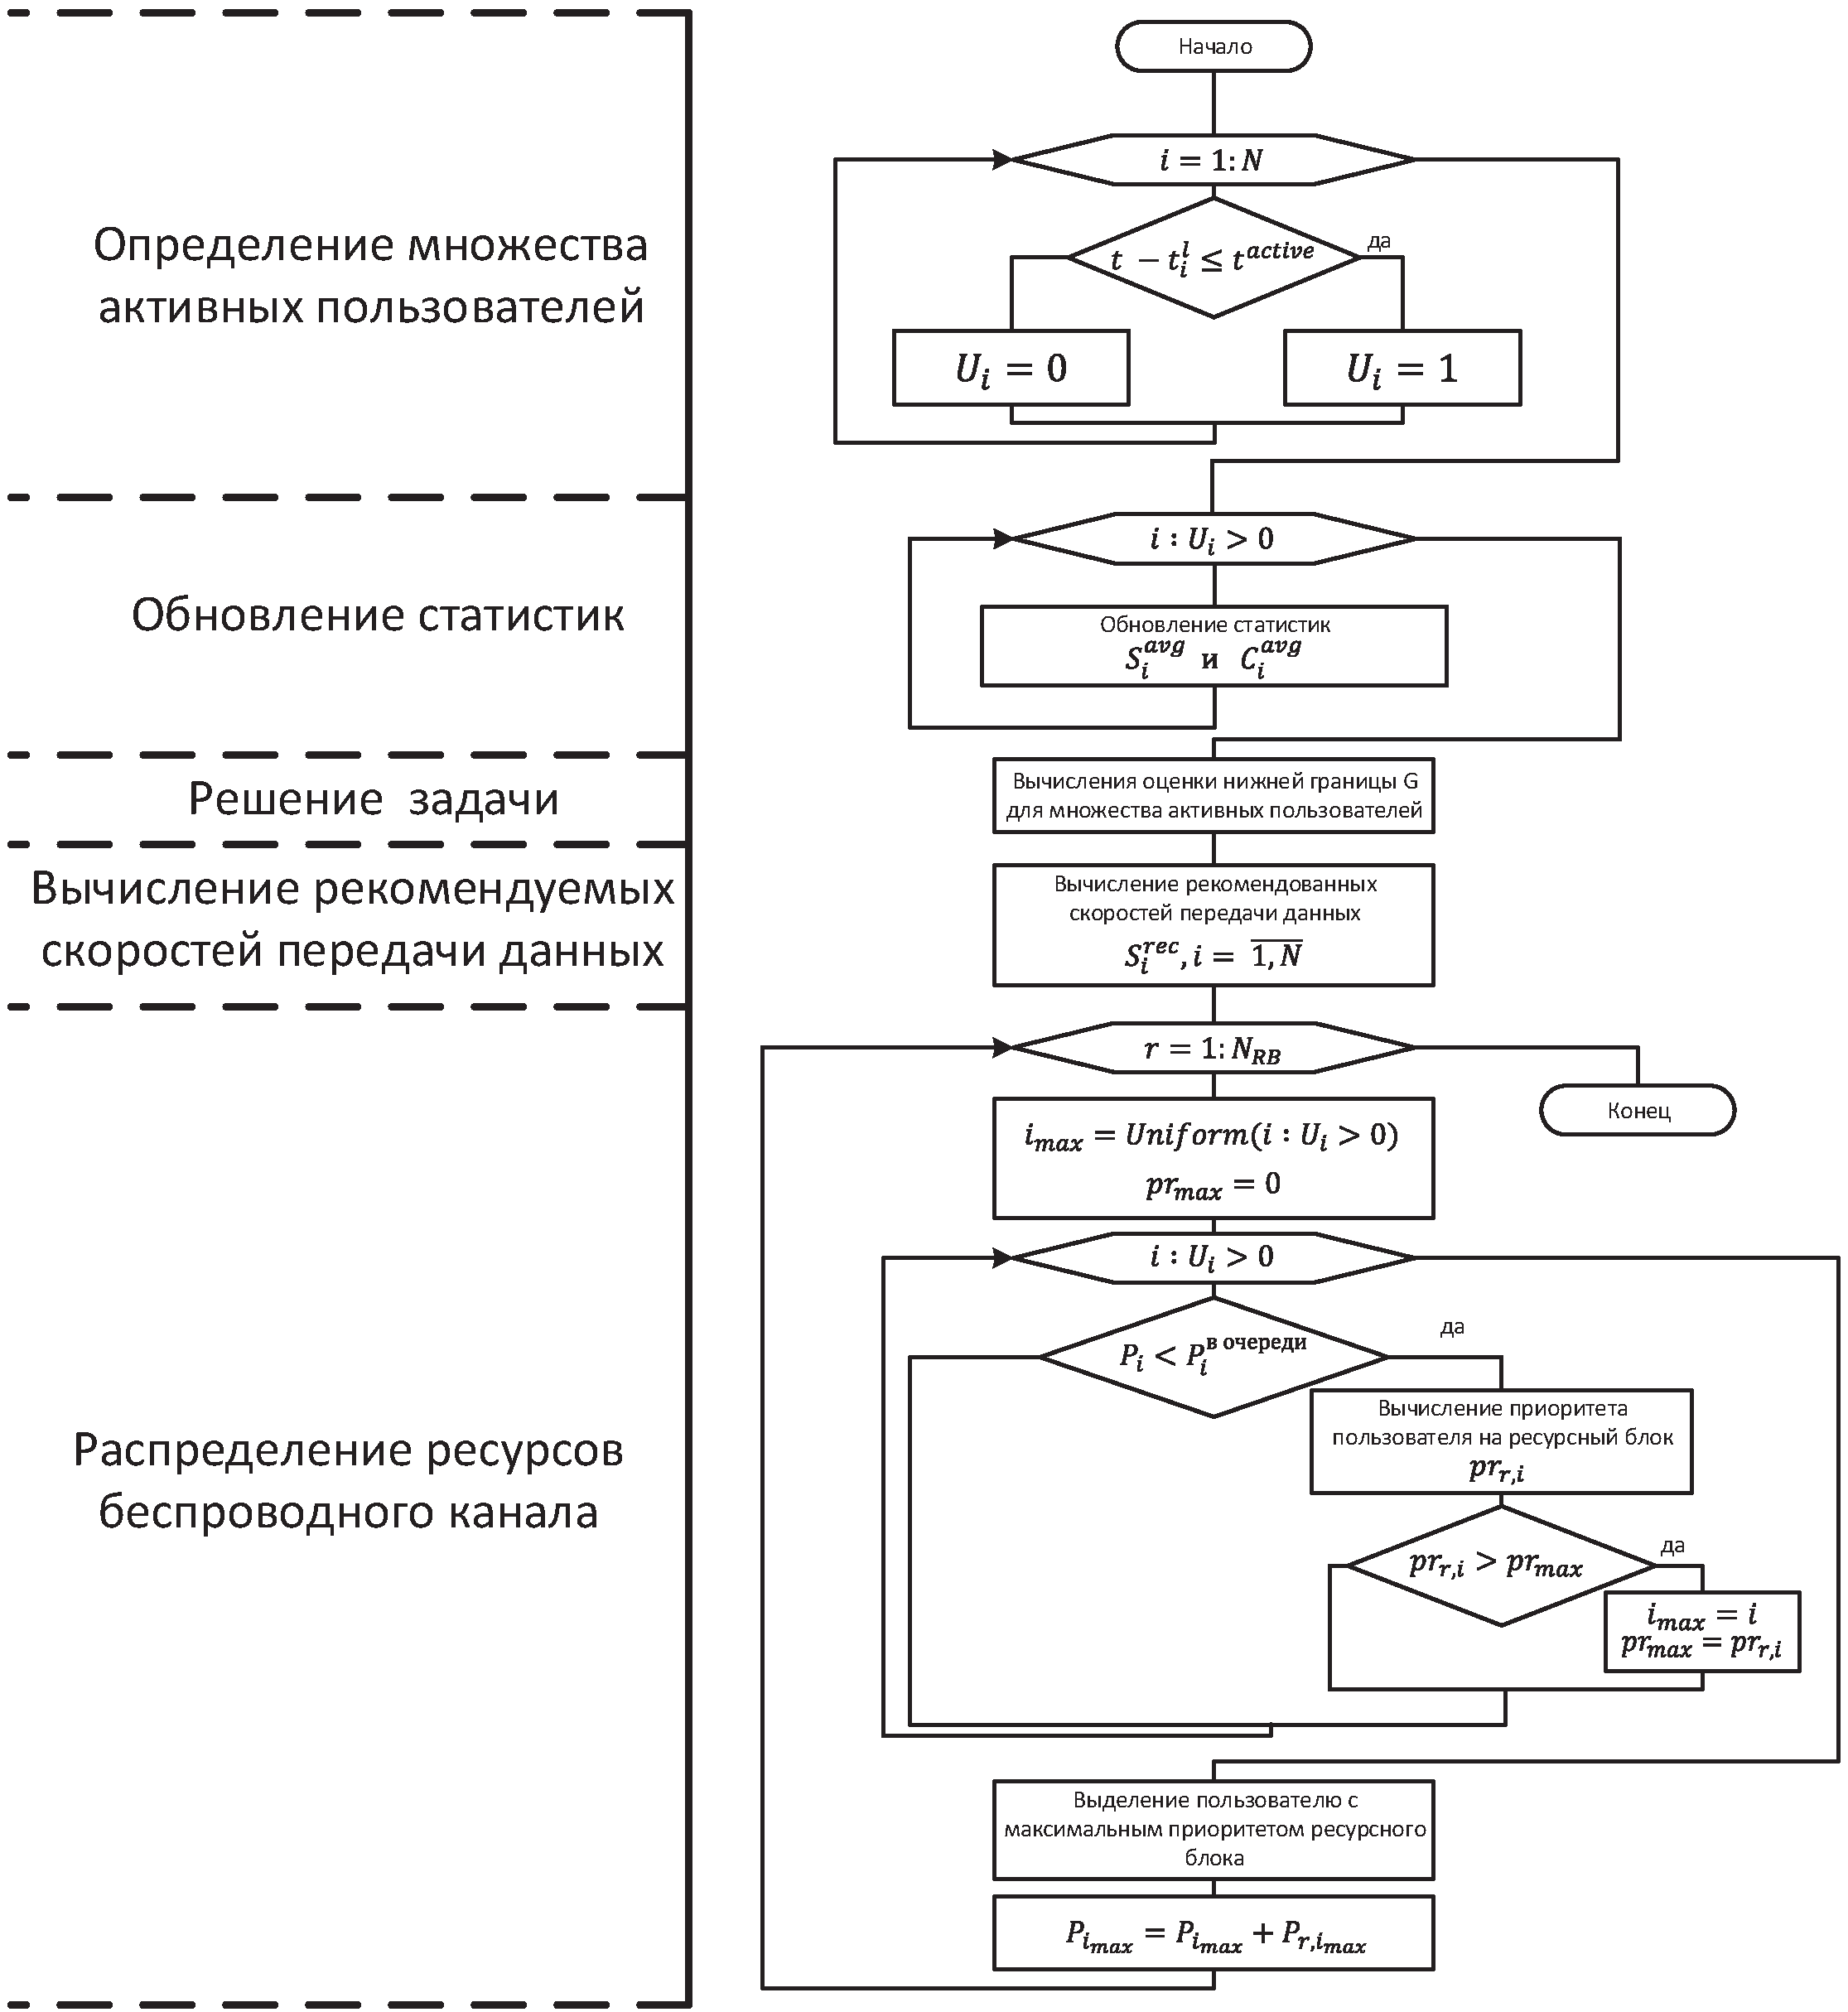
\includegraphics[width=\textwidth]{/Chapter3/hScheduler.pdf}
\caption{Логика алгоритма совместного планирования распределения ресурсов для неадаптивных видеопотоков}
\label{fig:HScheduler}
\end{center}
\end{figure}

Используя описанные ранее результаты, предлагается алгоритм планирования, выполняемый в каждый интервал планирования, состоящий из четырех шагов (рисунок~\ref{fig:HScheduler}):
\begin{itemize}
	\item \textbf{Определение множества активных пользователей}. На данном шаге все пользователи разделяются на два подмножества: активные и неактивные, в соответствии с выражением (\ref{eq:activityEstimation}).
	\item \textbf{Обновление статистик}. Для множества активных абонентов обновляются значения статистик в соответствии с выражениями (\ref{eq:CEstimation}) и (\ref{eq:SEstimation}).
	\item \textbf{Решение оптимизационной задачи}. Нахождение решения оптимизационной задачи (\ref{eq:optim_problem_g}) для множества активных пользователей пользователей: $\hat{G}(t) = \{\hat{g}_i(t), i \in \mathcal{U}\}$, при $K_i = \hat{R_i}(t) / C^{avg}_i(t)$ и $\gamma = 1$;
	\item \textbf{Вычисление рекомендуемых скоростей передачи данных}. Вычисление рекомендуемых скоростей передачи данных для всех активных пользователей в соответствии с выражением (\ref{eq:SReqCalc}).
	\item \textbf{Распределение ресурсов беспроводного канала}. Выделение ресурсов беспроводного канала в соответствии с предложенным механизмом обеспечения рекомендованной скорости (\ref{eq:PriorFunction}). На данном шаге также производится контроль за объемом выделенных ресурсов с целью предотвращения выделения ресурсных блоков, которые не могут быть использованы пользователем ввиду отстутствия достаточного объема информации в очереди на базовой станции.
\end{itemize}

В результате настоящего подраздела предложен алгоритм планирования распределения частотно-временных ресурсов беспроводного канала связи для централизованных систем передачи информации. Производительность предложенного алгоритма планирования будет продемонстрирована в подразделе \ref{chap3:NumericalExample} в сравнении с известными решениями и найденной в подразделе \ref{chap3:LowerBoundForG} нижней границей.

\section{Численный пример}
\label{chap3:NumericalExample}

Демонстрация результатов настоящей работы является нетривиальной задачей ввиду сложности анализируемой системы и невозможности постановки натурных экспериментов, так как оборудование централизованных сетей связи (базовые станции, опорная сеть оператора и т.д.) недоступно для рядового исследователя, что приводит к необходимости поиска платформы для моделирования. Таким образом, настоящий подраздел решает две задачи:
\begin{itemize}
	\item Выбор стандарта беспроводной централизованной системы передачи информации, на котором будут демонстрироваться полученные результаты;
	\item Выбор платформы и сценария моделирования, обладающих достаточной достоверностью получаемых результатов моделирования.
\end{itemize}

Изначально проведем анализ современных стандартов связи, которые соответствуют рассматриваемой в настоящей работе модели системы (раздел \ref{chap2}). В настоящий момент времени наиболее известными технологиями, соответствующих введенной модели системы, являются два стандарта связи: IEEE 802.16 или \textit{Worldwide Interoperability for Microwave Access} (WiMAX) \cite{wimax_std} и \textit{Long-Term Evolution Advanced} (LTE) \cite{lte_std}. В соответствии с анализом распространенности технологий связи, проведенным компанией Cisco, в настоящее время сети связи, построенные на основе стандарта WiMAX, не имеют широкого распространения, в свою очередь системы стандарта LTE получили широчайшее распространение в мире \cite{Cisco}. Более того, стандарт связи LTE постоянно обновляется и дополняется. Основываясь на сказанном выше, результаты настоящей работы будут демонстрироваться на основе стандарта связи LTE. Важно отметить, что полученные в настоящей работе результаты применимы ко всем беспроводным централизованным системам связи, а в данном разделе лишь демонстрируются на примере самого распространенного стандарта, удовлетворяющего модели системы.

Следующим шагом необходимо выбрать платформу моделирования систем стандарта LTE. В настоящий момент времени существует несколько возможных платформ:
\begin{itemize}
	\item \textit{Maltab}. Компанией MathWorks предлагается модуль анализа сетей стандарта LTE: LTE System Toolbox в рамках пакета Simulink, распространяемый с платной подпиской \cite{Matlab}. Данный модуль позволяет оценивать характеристики беспроводного канала связи для данного стандарта путем имитационного моделирования. Однако, в настоящем пакете не представлены реализации вышележащих уровней стека протоколов беспроводного соединения стандарта LTE и опорной сети оператора. Данный факт приводит к невозможности использования данной платформы для демонстрации результатов настоящей работы.
	\item \textit{Opnet LTE Simulation}. Компания Opnet предлагает платформу для моделирования сетей стандарта LTE с платной подпиской OPNET LTE SIMULATION \cite{Opnet}. Данная платформа включает в себя полный стек проколов беспроводной связи и опорной сети оператора, однако, исходный код данного проекта является закрытым и его невозможно дополнить клиент-серверными приложениями, осуществляющие загрузку и демонстрацию видео. Следовательно, использовать данну платформу невозможно для демонстрации полученных результатов.
	\item Система моделирования \textit{NS-3}. В 2012 году была создана низкоуровневая система моделирования сетевых протоколов с открытым исходным кодом NS-3 \cite{ns-3}. Данная система моделирования реализована на языке программирования С++ и ее компоненты соотвествует стандартам связи. В NS-3 также реализован модуль стека протоколов LTE для беспроводной сети и опорной сети оператора, соответствующие стандарту \cite{lte_std}. Открытый исходный код позволяет производить дополнение и гибкую настройку системы для широкого спектра задач.
\end{itemize}

Таким образом, результаты настоящей работы будут демонстрироваться с использованием системы моделирования NS-3 для стандарта связи LTE. Достоверность полученных результатов обеспечивается соответствием системы моделирования стандарту связи LTE.

Для адаптации системы моделирования NS-3 был решен ряд технических задач:
\begin{itemize}
	\item Реализация приложений видео контент сервера и клиентского приложения, соответствующие стандарту DASH (подраздел \ref{chap1:VideoPlayers});
	\item Реализация в модуле базовой станции LTE системы анализа трафика DPI, позволяющая в каждый момент времени моделирования получить информацию о виде трафика и его характеристиках;
	\item Реализация механизмов оценки характеристик передачи информации для пользователей, подключенных к базовой станции, в соответствии с решениями, представленными в подразделе \ref{chap3:NonAdaptiveScheduler};
	\item Реализация алгоритма планирования, предложенного в подразделе \ref{chap3:NonAdaptiveScheduler}.
\end{itemize}

Следующим важным шагом для демонстрации результатов является выбор сценария моделирования. В настоящей работе автор следовал указаниями, представленным в \cite{simulation}. Рассматривается работа одной соты, в которой находится $N$ пользователей на прямой линии с равным расстояниям друг от друга (рисунок \ref{fig:scenario}). Расстояние между соседними пользователями вычисляется следующим образом:
$$\Delta x = \frac{X_{max}}{N+1},$$
где $X_{max}$~--~максимально возможная удаленность пользователей от базовой станции.

\begin{figure}[htbp]
\begin{center}
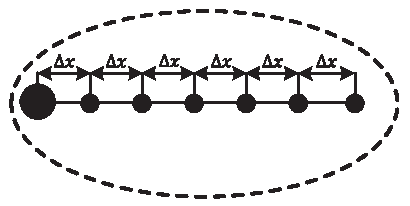
\includegraphics[width=0.7\textwidth]{/Chapter3/scenario.pdf}
\caption{Сценарий моделирования}
\label{fig:scenario}
\end{center}
\end{figure}

В данном сценарии моделирования рассматривается канал связи с плоскими замираниями (подраздел \ref{chap2:RadioChannel}). Для этого был сгенерирован случайный процесс, который изменяет затухание в канале от времени по всем доступным частотам для передачи. Таким образом затухание сигнала в канале от времени зависит от двух факторов: удаленности от базовой станции и плоскими замираниями в канале связи.

Полный список настроек сценария моделирования для каждого компонента модели системы представлен в таблице \ref{tab:SimParams}.

В сценарии моделирования наращивалось число абонентов до перехода системы в состоянии перегрузки (определение \ref{def:Congestion}). И производится сравнение на основе критерия $G$ (\ref{eq:gMetricGoal}) производительности известных алгоритмов планирования (\textit{Proportional Fair} и \textit{Round Robin}) с предложенным алгоритмом и найденной нижней границей. Результат проведенного сравнения представлен на рисунке \ref{fig:G_PLOT}.

\begin{figure}[htbp]
\begin{center}
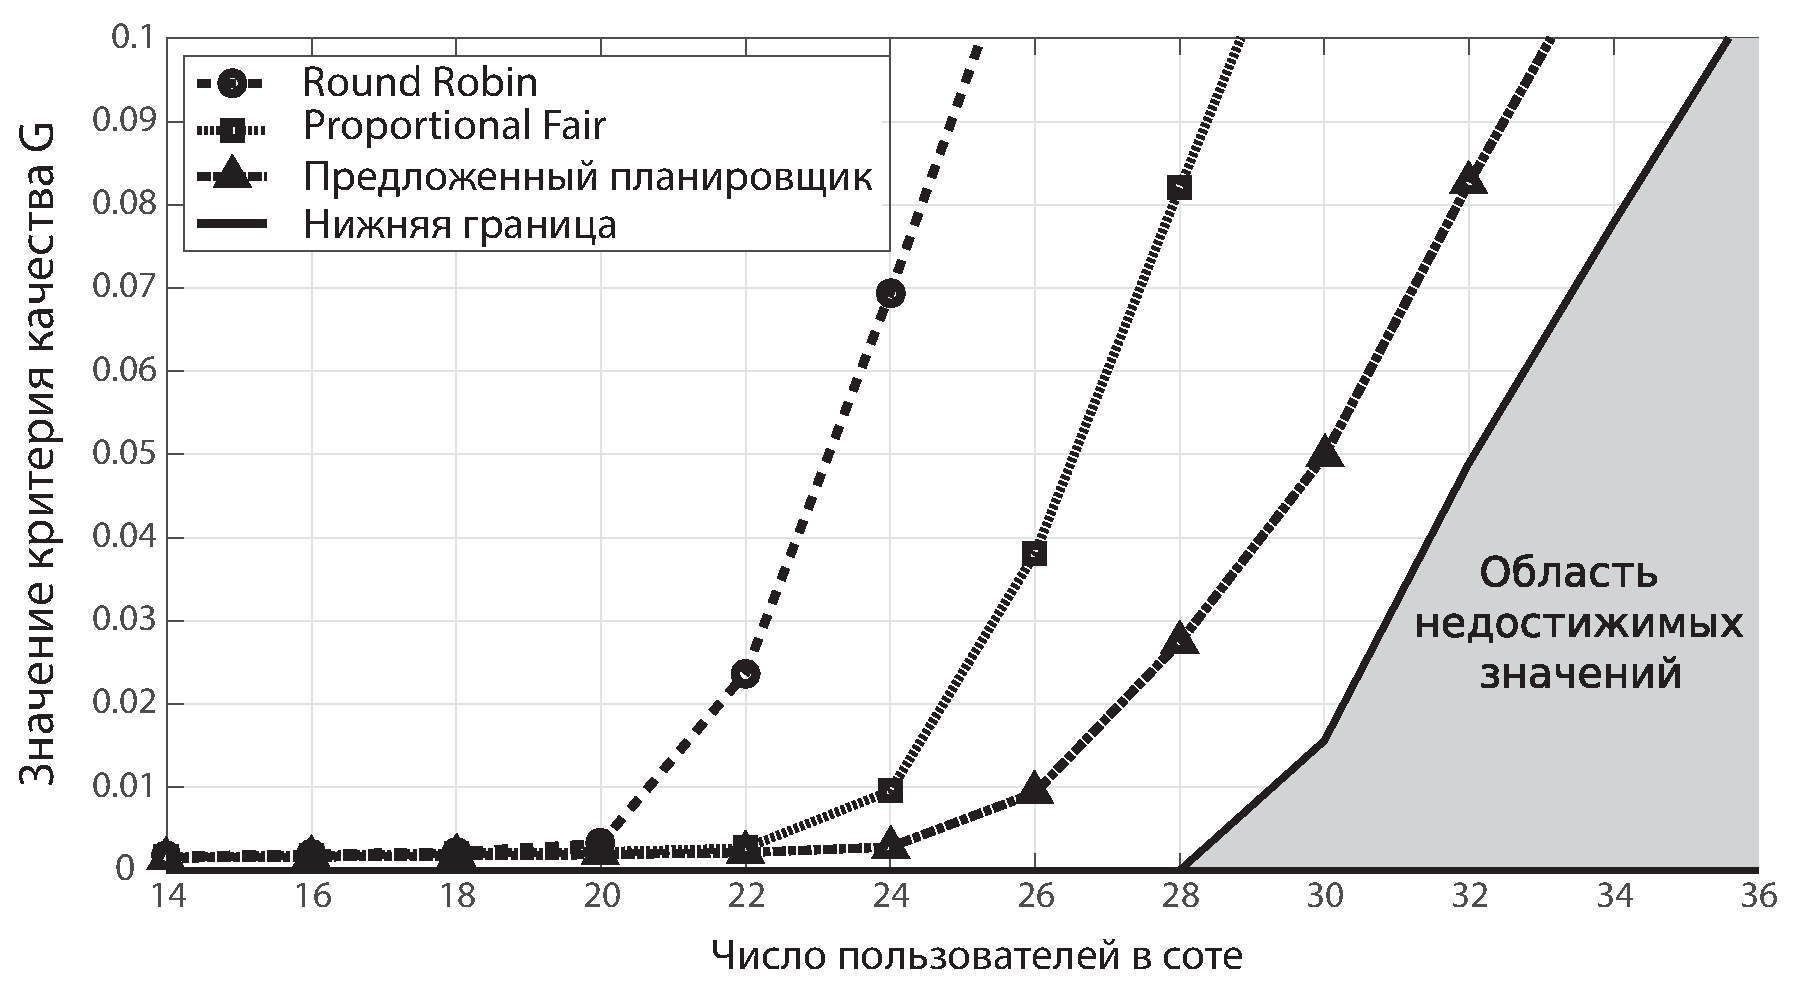
\includegraphics[width=\textwidth]{/Chapter3/G_PLOT.pdf}
\caption{Сравнение предложенного алгоритма планирования с известными планировщиками и найденной нижней границей}
\label{fig:G_PLOT}
\end{center}
\end{figure}

На рисунке \ref{fig:G_PLOT} приведена нижняя граница, характеризующая максимальную производительность алгоритмов планирования в настоящем сценарии моделирования. Заштрихованная область характеризует значения, которые не могут быть достигнуты любым планировщиком, удовлетворяющим допущениям введенных в подразделе \ref{chap2:Assumptions}: не существует планировщика, который при 30-ти пользователей в соте обеспечивает значения критерия качества восприятия $G$ равный $0.01$. Из рассмотрения рисунка \ref{fig:G_PLOT} следует, что предложенный алгоритм планирования показывает высокую производительность в сравнении со стандартными алгоритмами и нижней границей.

\section{Выводы по разделу}

Настоящий раздел был посвящен вопросам оптимизации передачи неадаптивных видеопоследовательностей в беспроводных централизованных сетях. В рамках раздела был выбран критерий качества восприятия: нормированное отношение длительности буферизации к просмотру (определение \ref{def:gMetric}), характерный для неадаптивного видео, и произведен его анализ. На основании данного критерия и модели системы, введенной в разделе \ref{chap2} была поставлена оптимизационная задача нелинейного программирования (\ref{eq:optim_problem_g}), решение которой характеризует максимально возможную производительность алгоритмов планирования при передаче неадаптивного видео. Далее было предложено решение данной задачи, путем ее сведения к обобщенной задачи о непрерывном рюкзаке, решение которой было найдено в настоящем разделе. Полученное решение характреризует нижнюю границу нормированного отношения длительности буферизации к просмотру для всевозможных алгоритмов планирования, удовлетворяющих введенных допущениям в подразделе \ref{chap2:Assumptions}, при передаче неадаптивных видеопотоков.

На основе найденного решения, обладающего низкой вычислительной сложностью, был предложен планировщик, с высокой производительностью в сравнении с существующими планировщиками и найденной нижней границей.

Основные результаты раздела могут быть сформулированы следующим образом:
\begin{itemize}
	\item Проведен анализ факторов, влияющих на восприятие неадаптивных видепотоков, и предложен критерий качества восприятия на основе нормированного отношения длительности буферизации к просмотру (подраздел~\ref{chap3:NonAdaptiveQoe});
	\item Произведена постановка оптимизационной задачи нелинейного программирования, характеризующей нижнюю границу для введенного критерия. Найдено решение с низкой вычислительной сложностью и предложен алгоритм расчета нижней границы для нормированного отношения длительности буферизации к просмотру по всевозможным алгоритмам планирования, удовлетворяющим допущениям из подраздела \ref{chap2:Assumptions} (подразделы \ref{chap3:NonAdaptiveOptimizationProblem}, \ref{chap3:GeneralizedFKSP} и \ref{chap3:LowerBoundForG});
	\item Предложен алгоритм планирования для неадаптивных видеопотоков, реализующий концепцию совместного планирования распределения ресурсов на базовой станции. Показано, что производительность предложенного планировщика превосходит известные решения и сравнима с нижней границей. Результаты настоящего раздела демонстрировались в системе моделирования NS-3, для стандарта связи LTE, соответствующего модели системы передачи информации, введенной в разделе \ref{chap2} (подразделы \ref{chap3:NonAdaptiveScheduler} и \ref{chap3:NumericalExample}).
\end{itemize}
           % Раздел 3
\chapter{АНАЛИЗ ПРОИЗВОДИТЕЛЬНОСТИ БЕСПРОВОДНЫХ ЦЕНТРАЛИЗОВАННЫХ СЕТЕЙ ДЛЯ ПЕРЕДАЧИ АДАПТИВНЫХ ВИДЕОПОТОКОВ}
\label{chap4}

\section{Вводные замечания}
\label{chap4:Intro}

В разделе \ref{chap3} было проведено исследование максимально возможной производительности алгоритмов распределения ресурсов радиоканала на базовой станции в беспроводных централизованных сетях для передачи неадаптивных видеопотоков. Несмотря на широкое использование неадаптивных видеоплееров для передачи видеоданных, в настоящее время все большую популярность приобретают адаптивные технологии передачи видео по протоколу HTTP (подраздел \ref{chap1:VideoPlayers}). Наиболее ярким представителем подобных технологий является стандарт Dynamic Adaptive Streaming over HTTP (DASH) \cite{dash_standard,conviva}.

Данная технология позволяет пользовательскому устройству подобрать качество видео под конкретные условия в сети передачи видеоданных. Это может привести к снижению нагрузки на сеть передачи информации за счет адаптации видеоряда.
% Исключительным качеством данной технологии является инвариантность по отношению к сети передачи информации, обеспечиваемая совместным использованием сетевых протоколов HTTP (уровень приложения) и TCP (транспортный уровень). Однако, использование настоящей технологи вносит небольшую избыточность при передачи видео из-за использования квитирования пакетов протоколом TCP.
В настоящий момент широкое распространение стандарта DASH обеспечивается его использованием сервисом хранения видеоконтента YouTube, который является крупнейшим хранилищем видеоданных в сети Интернет.

Настоящий раздел посвящен аналитическому исследованию производительности беспроводных централизованных систем передачи информации с доминированием передачи видео по протоколу прикладного уровня HTTP с возможностью его адаптации под специфичные условия сети передачи информации. Данный раздел неотступно следует системе допущений, введенной в подразделе \ref{chap2:Assumptions}.

В начале раздела предлагается критерий качества обслуживания для адаптивных видеопотоков. Далее формулируется оптимизационная задача и предлагается нижняя граница для введенного критерия по всем возможным алгоритмам распределения ресурсов беспроводного канала и адаптации видеоряда. В завершении предлагается численный пример, демонстрирующий производительность стандартных алгоритмов планирования распределения ресурсов беспроводного канала в сравнении с найденной нижней границей.

%Основные результаты данного раздела опубликованы в работе.

\section{Критерии качества восприятия адаптивного видеопотока}
\label{chap4:AdaptiveQoe}

В подразделе \ref{chap3:NonAdaptiveQoe} был проведен анализ основных объективных показателей воспроизведения видеоданных, влияющих на оценку качества восприятия видеопотока и описанных ранее в подразделах \ref{chap1:VideoMOS} и \ref{chap2:VideoTrafficModel}:
\begin{itemize}
	\item Битовая скорость потока, характеризующая качество видео;
	\item Длительность буферизации, включающая в себя длительности всех начальных и повторных буферизаций во время просмотра;
	\item Гладкость воспроизведения видеоряда.
\end{itemize}
Рассмотрим каждый из них с позиции адаптивной передачи видеоданных.

Принципиальным отличием адаптивных видеоплееров от неадаптивным является наличие механизма подбора репрезентации видео в зависимости от характеристик канала передачи информации или адаптации репрезентации (подраздел \ref{chap1:VideoPlayers}). Основной целью механизма адаптации репрезентации является минимизация длительности буферизации (начальные и повторные буферизации в течении просмотра видео), так как данный фактор имеет сильное влияние на качество восприятия видео пользователем. Однако, помимо общей длительности буферизации, определяющую роль при оценке качества восприятия выполняет битовая скорость потока, характеризующая качество видеоряда (подраздел \ref{chap1:VideoMOS}). Это демонстрирует сложную взаимосвязь между битовой скоростью потока и длительностью буферизации при построении управления для адаптивных видеоплееров.

Продемонстрируем эту взаимосвязь на примере. Пусть для некоторого мобильного пользователя скорость получения информации равняется $0.65$ Мбит/с и постоянна во времени. Исходя из таблицы \ref{tab:youtubeBr}, данная скорость получения информации может обеспечить просмотр видео в качестве 360p ($0.45$ Мбит/с) без возникновения повторных буферизаций во время просмотра, или в качестве 480p ($0.7$ Мбит/с) с наличием повторными буферизаций, длительностью $5\%$ от длительности просмотра. Однако, битовая репрезентация задает верхнюю границу удовлетворенности пользователя при просмотре: для данного примера при просмотре видео в идеальных условиях (минимально возможная длительность начальной буферизации и отсутствие повторных) в качестве 360p значение MOS (методология U-vMOS) не может превышать значения 3, а для 480p~--~3.64. Следовательно, обеспечение пользователю просмотра видео в качестве 360p без повторных буферизаций не приводит к его достаточной удовлетворенности качеством обслуживания, так как пользователь считается удовлетворенным если величина MOS превышает значение 3.

Приведенный выше пример демонстрирует важную специфику организации управления полезной скоростью получения информации для адаптивных видеоплееров: \textit{безусловная минимизация общей длительности буферизации не приводит к максимизации удовлетворенности пользователя просмотром видео}. Что приводит к необходимости учета битовой скорости потока в критерии качества восприятия для адаптивных видеоплееров.

Из анализа работы адаптивных видеоплееров, проведенного в подразделе \ref{chap1:VideoPlayers}, следует, что гладкость воспроизведения видеоряда обеспечивается алгоритмом выбора репрезентации, установленном на видеоплеере и ограничено сверху некоторой величиной (подраздел \ref{chap2:VideoTrafficModel}).

Таким образом, при формировании критерия качества восприятия адаптивного видеопотока необходимо учитывать два фактора воспроизведения: длительность буферизаций и битовую скорость потока.

В настоящем разделе качество восприятия фактора длительности буферизации будет оцениваться на основе критерия отношение длительностей буферизации и просмотра (определение~\ref{def:BWTR}): $$q_i = \lim\limits_{T\rightarrow\infty} \frac{b_i^T}{w_i^T},$$
где $b_i^T$~--~общая длительность буферизации пользователя $i$ за время $T$, $w_i^T$~--~общая длительность просмотра видео пользователем $i$ за время $T$.

Данный критерий позволяет оценить удовлетворенность пользователя:
$$q_i=
\begin{cases}
0, & \text{пользователь $i$ удовлетворен просмотром}\\
\varepsilon > 0 & \text{пользователь $i$ наблюдает негативные эффекты при просмотре}\\
\end{cases}.
$$
Значение критерия качества восприятия $q_i$ обратно пропорционально удовлетворенности пользователя просмотром. Впервые критерий качества $q_i$ был рассмотрен в работе \cite{Bakin_Globecom}.

В качестве критерия качества восприятия фактора длительности буферизаций, описывающего систему в целом, было выбрано среднее значение отношение длительностей буферизации и просмотра всех пользователей в системе (\ref{eq:qMetricGoal}). На значение критерия (\ref{eq:qMetricGoal}) оказывают влияние алгоритм планирования распределения ресурсов $A$, установленный на базовой станции, и алгоритм адаптации битовой репрезентации $B$, установленный на пользовательских устройствах, принадлежащим множествам $\mathcal{A}$ и $\mathcal{B}$ соответственно (подраздел \ref{chap2:Assumptions}).

\begin{equation}
	\label{eq:qMetricGoal}
	\bar{q}\left(A, B\right)=\frac{1}{N}\left(\sum\limits_{i=1}^{N} {q_i\left(A,B\right)}\right).
\end{equation}

В отличии от критерия качетсва восприятия, представленного в подразделе \ref{chap3:NonAdaptiveQoe}, наличие адаптации видеоряда вносит более сложную зависимость качества восприятия от параметров системы. Она выражается в наличии обратной связи при взаимной работе алгоритмов $A$ и $B$: исходя из скорости получения информации обеспеченной алгоритмом $A$, алгоритм $B$ выбирает битовую скорость для заказываемых сегментов, которая влияет на загрузку беспроводного канала и скорость передачи информации.

Средняя битовая скорость видеопотока всех пользователей будет использоваться для оценки фактора качества репрезентации.

\begin{equation}
	\label{eq:rateMetricGoal}
	\overline{R}\left(A,B\right) = \frac{1}{N}\left(\sum\limits_{i=1}^{N} {\tilde{R}_i\left(A,B\right)}\right),
\end{equation}
где $\tilde{R}_i$~--~математическое ожидание битовой скорости видеопотока пользователя $i$ (подраздел \ref{chap2:InterrelationVideoParams}).

В данном подразделе был проведен анализ основных факторов, влияющих на качество восприятия адаптивного видеопотока. Результатом данного анализа является выбор двух критериев качества: среднее значение отношения длительностей буферизации и просмотра (\ref{eq:qMetricGoal}) и средняя битовая скорость видеопотока всех пользователей в системе (\ref{eq:rateMetricGoal}). На основе данных критериев будет сформирована оптимизационная задача для исследования максимальной производительности беспроводных централизованных сетей связи при передаче адаптивных видеопоследовательностей.

\section{Постановка оптимизационной задачи}
\label{chap4:AdaptiveOptimizationProblem}

В данном подразделе производится постановка и анализ оптимизационной задачи для исследования максимально возможной производительности беспроводных централизованных сетей связи при передаче адаптивных видеопоследовательностей. В подразделе \ref{chap4:AdaptiveQoe} было произведено рассмотрение факторов, влияющих на качество восприятия адаптивного видео, и выделены два основных: (\ref{eq:qMetricGoal}) и (\ref{eq:rateMetricGoal}). Настоящий подраздел построен следующим образом: в начале предлагается обобщенный критерий качества, объединяющий критерии (\ref{eq:qMetricGoal}) и (\ref{eq:rateMetricGoal}). Далее предлагается обобщенный критерия качества восприятия и предлагается оптимизационная задача. В завершении подраздела производится анализ оптимизационной задачи.

Важным выводом из подраздела \ref{chap4:AdaptiveQoe} является необходимость условной оптимизации фактора длительности буферизации: $\bar{q}\left(\mathcal{A}, \mathcal{B}\right)$, при передаче адаптивных видеопотоков. Вторым фактором, влияющим на качество восприятия, была выделена средняя битовая скорость видео по всем пользователям в системе $R_{avg}$, выступающая в роли ограничения при минимизации фактора длительности буферизации. В настоящем разделе обобщенный критерий качества обслуживания для адаптивного видеоряда вводится в следующем виде:

\begin{equation}
Q = \inf\limits_{A,B: \overline{R}\left(A,B\right) \geq R_{avg}, A \in \mathcal{A}, B \in \mathcal{B}} \overline{q}\left(A,B\right).
\label{eq:extr_param}
\end{equation}

Таким образом, целью настоящего раздела является нахождение нижней границы отношения длительностей буферизации и просмотра по всем возможным алгоритмам планирования распределения ресурсов на базовой станции $\mathcal{A}$ и алгоритмам выбора репрезентации $\mathcal{B}$, удовлетворяющих допущениям введенных в подразделе \ref{chap2:Assumptions}, таким что среднее средняя битовая скорость видеопотоков превышает величину $R_{avg}$.

Важно отметить, что в настоящем разделе используется система допущений из подраздела \ref{chap2:Assumptions} без дополнительных изменений, что позволяет использовать утверждение~\ref{lem:GeneralConstrain} в виде, представленом в подразделе~\ref{chap2:InterrelationVideoParams}. Таким образом, оптимизационная задача для критерия качества (\ref{eq:extr_param}), описывающая максимальную производительность передачи адаптивных видеопотоков в беспроводных централизованных сетях, принимает следующий вид:

\begin{equation}
\begin{array}{l}
\text{ \textbf{Минимизировать:} } \frac{1}{N}\sum\limits_{i=1}^N q_i \\
\text{ \textbf{При условии:} }\\
\begin{cases}
\sum\limits_{i=1}^{N} {\left(1-\nu^R_i\nu^C_i\right)\frac{\tilde{R}_i \tilde{C}^{-1}_i }{q_i + \gamma_i}} -1 \leq 0 \\
-\frac{1}{N}\sum\limits_{i=1}^{N}\tilde{R}_i + R_{avg} \leq 0 \\
\tilde{R}_i \in \left[R_{min}, R_{max}\right], i=\overline{1,N} \\
-q_i \leq 0,\mbox{ }i=\overline{1,N} \\
\end{cases}
\end{array}.
\label{eq:optim_problem_q}
\end{equation}

Проведем анализ задачи (\ref{eq:optim_problem_q}) на качественном уровне. В настоящей оптимизационной задаче $2N$ переменных: $q = (q_1, q_2, \ldots, q_N)$ и $\tilde{R} = (\tilde{R_1}, \tilde{R_2}, \ldots, \tilde{R_N})$. Из вида первого ограничения следует, что оптимизационная задача (\ref{eq:optim_problem_q}) относится к классу задач нелинейного программирования. Важнейшим этапом анализа оптимизационных задач, определяющим возможные методы их решения, является определение подкласса задачи нелинейного: задачи выпуклого, вогнутого или невыпуклого программирования. Завершающая часть данного подраздела посвящена именно определению подкласса задачи (\ref{eq:optim_problem_q}).

Оптимизационная задача (\ref{eq:optim_problem_q}) обладает целевой функцией линейного вида и линейными ограничениями типа неравества, исключая первое ограничение, следовательно, тип задачи будет определяться видом первого ограничения. Стоит отметить, что данное ограничение это функция от $2N$ переменных. Для его анализа рассмотрим случай, когда в системе находится только один абонент ($N=1$), в данном случае число переменных уменьшается до двух. Для упрощения последующих математических выкладок в выражении (\ref{eq:GeneralConstrainOneUser}) номер абонента был опущен, так как в системе присутствует только он один.

\begin{equation}
\left(1-\nu^R\nu^C\right)\frac{\tilde{R} \tilde{C}^{-1} }{q + \gamma} -1.
\label{eq:GeneralConstrainOneUser}
\end{equation}

Определене вида функции от нескольких переменных возможно на основе матрицы Гессе \cite{convex_opt}. В зависимости вида матрицы Гессе возможно определить вид функции следующим образом: если матрица Гессе является
\begin{itemize}
	\item Положительно определенной во всех точках, то функция выпуклая;
	\item Отрицательно определенная во всех точках, то функция вогнутая;
	\item Не является знакоопределенной, то функция общего вида (невыпуклая).
\end{itemize}

Матрица Гессе $H(\cdot)$ для функции (\ref{eq:GeneralConstrainOneUser}) принимает следующий вид:
$$H(\tilde{R}, q)=
  \left[ {\begin{array}{ccc}
   0 & &-\frac{\left(1-\nu^R\nu^C\right)\tilde{C}^{-1}}{(q + \gamma)^2} \\
   & & \\
   -\frac{\left(1-\nu^R\nu^C\right)\tilde{C}^{-1}}{(q + \gamma)^2} & & \frac{\left(1-\nu^R\nu^C\right)\tilde{C}^{-1} \tilde{R}}{(q + \gamma)^3} \\
  \end{array} } \right]
$$

Так как матрица Гессе является симметричной относительно главной диагонали, то для определения ее знакоопределенности возможно использовать критерий Сильвестра: симметричная матрица является положительно определенной тогда и только тогда, когда все ее угловые миноры положительны, в случае неотрицательной определенности~--~больше или равны нулю. Отрицательная знакоопределенность симметричной матрицы задается чередованием знаков угловых миноров: отрицательный, положительный и т.д. В иных случаях матрица не является знакоопределенной \cite{convex_opt}.

Найдем значения угловых миноров $\Delta$ матрицы $H(\tilde{R}, q)$:
$$\Delta_1 = 0 \cdot \frac{\left(1-\nu^R\nu^C\right)\tilde{C}^{-1} \tilde{R}}{(q + \gamma)^3} = 0.$$
$$\Delta_2 = 0 \cdot \frac{\left(1-\nu^R\nu^C\right)\tilde{C}^{-1} \tilde{R}}{(q + \gamma)^3} - \left(-\frac{\left(1-\nu^R\nu^C\right)\tilde{C}^{-1}}{(q + \gamma)^2}\right)^2 = - \left(\frac{\left(1-\nu^R\nu^C\right)\tilde{C}^{-1}}{(q + \gamma)^2}\right)^2 < 0.$$

Так как значение $\left(1-\nu^R\nu^C\right)$ и сумма значений $q$ и $\gamma$ отличны от нуля (система допущений, подраздел \ref{chap2:Assumptions}), то значение второго углового минора ($\Delta_2$) строго отрицательно. Таким образом, основываясь на критерии Сильвестра, функция (\ref{eq:GeneralConstrainOneUser}) является функцией общего вида (невыпуклой). Следовательно, оптимизационная задача (\ref{eq:optim_problem_q}) относится к подклассу невыпуклых задач.

Критично важно отметить, что для задач невыпуклого программирования не существует стандартных методов или подходов к решению \cite{convex_opt,optimizations_methods}. Следовательно, решение оптимизационной задачи (\ref{eq:optim_problem_q}) является нетривиальной задачей. В настоящем разделе будет предложено решение данной задачи, которое будет основано на двуступенчатой оптимизации. Дальнейшая часть раздела будет построена следующим образом. На первом шаге будет представлено решение задачи выпуклого программирования на основе теоремы Каруша-Куна-Таккера (ККТ) с использованием метода \textit{<<water-filling>>}, описанного в \cite{convex_opt}. Далее будет предложен алгоритм вычисления нижней границы для оптимизационной задачи (\ref{eq:optim_problem_q}), который использует решение задачи на основе теоремы ККТ.

\section{Решение вспомогательной оптимизационной задачи выпуклого программирования на основе теоремы Каруша-Куна-Таккера}
\label{chap4:KktSolution}

В настоящем подразделе представлено решение задачи выпуклого программирования при наличии ограничения типа неравенств на основе теоремы Каруша-Куна-Таккера (ККТ) \cite{convex_opt,optimizations_methods}. Представленное решение было описано в работе \cite{Bakin_Globecom}.

Рассмотрим оптимизационную задачу следующего вида:

\begin{equation}
\begin{array}{l}
\text{ \textbf{Минимизировать:} } Q^{*} = \frac{1}{N}\sum\limits_{i=1}^N q_i \\
\text{ \textbf{При условии:} }\\
\begin{cases}
\sum\limits_{i=1}^{N} {\frac{\tilde{a}_i}{q_i + \gamma_i}} - L^{*} \leq 0\\
-q_i \leq 0 , i=\overline{1,N} \\
\end{cases}
\end{array},
\label{eq:optim_problem_bakin_lemma}
\end{equation}
где $\tilde{a}_i, i=\overline{1,N}$ и $L^{*}$ являются положительными и отличными от нуля числами.

\begin{lemma}
\label{lem:bakin_lemma}
Оптимальное значение $Q^{*}$ может быть получено на основе выражения (\ref{eq:optim_problem_bakin_lemma_solution}):
\emph{
\begin{equation}
Q^{*} =
\begin{cases}
0, & \text{если} \sum\limits_{i=1}^{N} {\left(\frac{\tilde{a}_i}{\gamma_i}\right)} \leq L^{*}\\
\frac{1}{N} \sum\limits_{i=1}^{N} {\mathrm{max} \left(\sqrt{\mu_0 \tilde{a}_i N}-\gamma_i, 0\right)}, & \mathrm{иначе} \\
\end{cases},
\label{eq:optim_problem_bakin_lemma_solution}
\end{equation}
}
\emph{
где $\mu_0$~--~решение уравнения (\ref{eq:optim_problem_bakin_lemma_solution_eq}):
\begin{equation}
\sum\limits_{i=1}^{N} {\frac{\tilde{a}_i}{\mathrm{max} \left(\sqrt{\mu_0 \tilde{a}_i N}, \gamma_i\right)}} - L^{*} = 0.
\label{eq:optim_problem_bakin_lemma_solution_eq}
\end{equation}
}
\end{lemma}

\begin{proof}

Из вида первого ограничения следует, что оптимизационная задача (\ref{eq:optim_problem_bakin_lemma}) относится к классу задач нелинейного выпуклого программирования. Следовательно, могут быть выписаны условия существования минимума ККТ, и существует единственная точка на многомерной плоскости, удовлетворяющая данным условиям. Теорема ККТ позволяет свести задачу выпуклого программирования к поиску седловой точки функции Лагранжа на множестве определенном ограничениями на неотрицательность значений множителей Лагранжа, принадлежность решения области допустимых значений \cite{optimizations_methods}.

Для оптимизационной задачи (\ref{eq:optim_problem_bakin_lemma}) найдем функцию Лагранжа $\mathcal{L}(\cdot)$:

\begin{equation}
\mathcal{L} (\boldsymbol{q}, \boldsymbol{\mu}) = \frac{1}{N} \sum\limits_{i=1}^{N}{q_i} + \mu_0 \left[ \left(\sum\limits_{i=1}^{N} {\frac{\tilde{a}_i}{q_i + \gamma_i}}\right) - L^{*}\right] - \mu_i q_i,
\label{eq:LagrangeFucntion}
\end{equation}
где $\boldsymbol{q}=(q_1, q_2, \ldots, q_N)$ и $\boldsymbol{\mu} = (\mu_0, \mu_1, \ldots, \mu_N)$ являются векторами длины $N$ и $(N+1)$ соответственно. Вектор $\boldsymbol{\mu}$ используется для обозначения множителей Лагранжа.

На основе (\ref{eq:LagrangeFucntion}), условия существования решения задачи (\ref{eq:optim_problem_bakin_lemma}) Каруша-Куна-Таккера представлены следующей системой:
\begin{equation}
\label{eq:KKT}
\begin{cases}
\frac{1}{N} - \mu_0 \frac{\tilde{a}_i}{(q_i + \gamma_i)^2} - \mu_i = 0, i = \overline{1,N} & \boldsymbol{\mathrm{Стационарность}}\\
-q_i \leq 0, i = \overline{1,N} & \boldsymbol{\mathrm{Выполнимость \quad 1}}\\
\sum\limits_{i=1}^{N} {\frac{\tilde{a}_i}{q_i + \gamma_i}} - L^{*} \leq 0 & \boldsymbol{\mathrm{Выполнимость \quad 2}}\\
\mu_j \geq 0, j = \overline{0,N} & \boldsymbol{\mathrm{Неотрицательность}}\\
\mu_i q_i = 0, i = \overline{1,N} & \boldsymbol{\mathrm{Дополняющая \quad нежесткость \quad 1}}\\
\mu_0 \left[ \left(\sum\limits_{i=1}^{N} {\frac{\tilde{a}_i}{q_i + \gamma_i}}\right) - L^{*}\right] = 0 & \boldsymbol{\mathrm{Дополняющая \quad нежесткость \quad 2}}\\
\end{cases}
\end{equation}

Теорема ККТ утверждает, что решение оптимизационной задачи (\ref{eq:optim_problem_bakin_lemma}) удовлетворяет всем условиям, представленным в системе (\ref{eq:KKT}). Одновременно с этим, выпуклость задачи обеспечивает единственность решения настоящей системы. Важно отметить, что условия ККТ могут быть применены и к задачам невыпуклого программирования, однако, в таком случае может существовать несколько возможных решений систем, аналогичных (\ref{eq:KKT}), так как в таких задачах возможно будет существовать множество локальных экстремумов. Данный факт приводит к необходимости организации перебора по полученным решениям для поиска глобального экстремума при использовании подхода на основе условий ККТ для задач невыпуклого программирования.

В обозначениях к системе (\ref{eq:optim_problem_bakin_lemma}) использовался адаптированный перевод англоязычных терминов:
\begin{itemize}
\item \textit{<<Stationarity>>}~--~\textbf{Стационарность}. Равенство градиента функции Лагранжа нулю;
\item \textit{<<Primal feasibility>>}~--~\textbf{Выполнимость}. Ограничения типа неравенства в каноническом виде;
\item \textit{<<Dual feasibility>>}~--~\textbf{Неотрицательность}. Ограничение на положительность значений множителей Лагранжа;
\item \textit{<<Complimentary slackness>>}~--~\textbf{Дополняющая нежесткость}.
\end{itemize}

Продолжим рассмотрение условий существования экстремума (\ref{eq:optim_problem_bakin_lemma}). Из условия \textbf{Стационарность} выразим значение $\mu_i$:
$$\mu_i = \frac{1}{N} - \mu_0 \frac{\tilde{a}_i}{(q_i + \gamma_i)^2}, i = \overline{1,N}.$$

Следовательно, условие \textbf{Дополняющая нежесткость 1} преобразуется к виду:
\begin{equation}
q_i \left[\frac{1}{N} - \mu_0 \frac{\tilde{a}_i}{(q_i + \gamma_i)^2}\right] = 0, i = \overline{1,N}.
\label{eq:interStep1}
\end{equation}
Уравнение (\ref{eq:interStep1}) задает зависимость значений $q_i$ от значения только одного множителя Лагранжа $\mu_0$. Проведем последовательный анализ выражения (\ref{eq:interStep1}) для конкретного пользователя $i$ в зависимости от значений $\mu_0$.

Пусть $\mu_0 \in \left[0, \frac{\gamma_i^2}{\tilde{a_i N}}\right)$, тогда выражение $\left[\frac{1}{N} - \mu_0 \frac{\tilde{a}_i}{(q_i + \gamma_i)^2}\right]$, равное $\mu_i$, принимает значения строго больше нуля. Следовательно, при данных значениях $\mu_0$, выражение (\ref{eq:interStep1}) имеет единственное решение $q_i = 0$.

Если $\mu_0 \in \left[\frac{\gamma_i^2}{\tilde{a_i N}},\infty\right)$, то значение в квадратных скобках (\ref{eq:interStep1}), равное $\mu_i$, принимает отрицательное значение при $q_i = 0$, однако, в соответствии с условием \textbf{Неотрицательность}, $\mu_i \geq 0$. Следовательно, при данных значениях $\mu_0$ решением уравнения (\ref{eq:interStep1}) является $q_i = \sqrt{\mu_0 \tilde{a}_i N}-\gamma_i$. Объединяя два полученных выше результата анализа, решение уравнения (\ref{eq:interStep1}) определяется следующим выражением:

\begin{equation}
q_i  = \mathrm{max} \left(\sqrt{\mu_0 \tilde{a}_i N}, \gamma_i \right).
\label{eq:SolutionStep1}
\end{equation}

Таким образом, задача нахождения значений вектора $\boldsymbol{q}$ может быть сведена к нахождению одного значения множителя Лагранжа $\mu_0$. Значение $\mu_0$ может быть получено из решения условия \textbf{Дополняющая нежесткость 2}, подставив в него (\ref{eq:SolutionStep1}) получим следующее уравнение:
$$\mu_0 \left[\sum\limits_{i=1}^{N} {\frac{\tilde{a}_i}{\mathrm{max} \left(\sqrt{\mu_0 \tilde{a}_i N}, \gamma_i\right)}} - L^{*}\right] = 0.$$

Данное уравнение имеет два возможных решения:
\begin{itemize}
	\item $\mu_0 = 0$. В данном случае $\forall i: q_i = 0$, если при данных значениях вектора $\boldsymbol{q}$ выполняется условие \textbf{Выполнимость 2}.
	\item $\mu_0$ находится из решения уравнения (\ref{eq:optim_problem_bakin_lemma_solution_eq}).
\end{itemize}
Настоящий факт завершает доказательство.
\end{proof}

Описанный подход нахождения решения системы условий существования экстремума в англоязычной литературе известен под названием \textit{water-filling} и представлен в \cite{convex_opt}.

Обобщая сказанное выше, решение оптимизационной задачи (\ref{eq:optim_problem_bakin_lemma}) может быть получено из решения уравнения (\ref{eq:optim_problem_bakin_lemma_solution_eq}). Важно отметить, что (\ref{eq:optim_problem_bakin_lemma_solution_eq}) обладает монотонной завистью от значения $\mu_0$. Для нахождения решения данного уравнения может быть предложена двухэтапная численная процедура (алгоритм \ref{alg:algorithm_numerical_solution}).

\begin{algorithm}
  \caption{: Численное решение уравнения (\ref{eq:optim_problem_bakin_lemma_solution_eq})}
	\label{alg:algorithm_numerical_solution}
  \begin{algorithmic}[1]
	 \item Найти отрезок $[k,r]:\begin{cases}
		\sum\limits_{i=1}^{N} {\frac{\tilde{a}_i}{\mathrm{max} \left(\sqrt{k \tilde{a}_i N}, \gamma_i\right)}} \geq L^{*} \\
		\sum\limits_{i=1}^{N} {\frac{\tilde{a}_i}{\mathrm{max} \left(\sqrt{r \tilde{a}_i N}, \gamma_i\right)}} \leq L^{*}
		\end{cases}.$
		\newline
		алгоритмом экспоненциального шага: удвоение значения $r$, до тех пор пока не найдется значение, удовлетворяющее условиям.
	 \item Найти решение уравнения (\ref{eq:optim_problem_bakin_lemma_solution_eq}) на отрезке $[k,r]$ алгоритмом дихотомии (деления отрезка пополам).
  \end{algorithmic}
\end{algorithm}
Графическое представление алгоритма \ref{alg:algorithm_numerical_solution} приведено на рисунке \ref{fig:numerical_alg}.

\begin{figure}[htbp]
\begin{center}
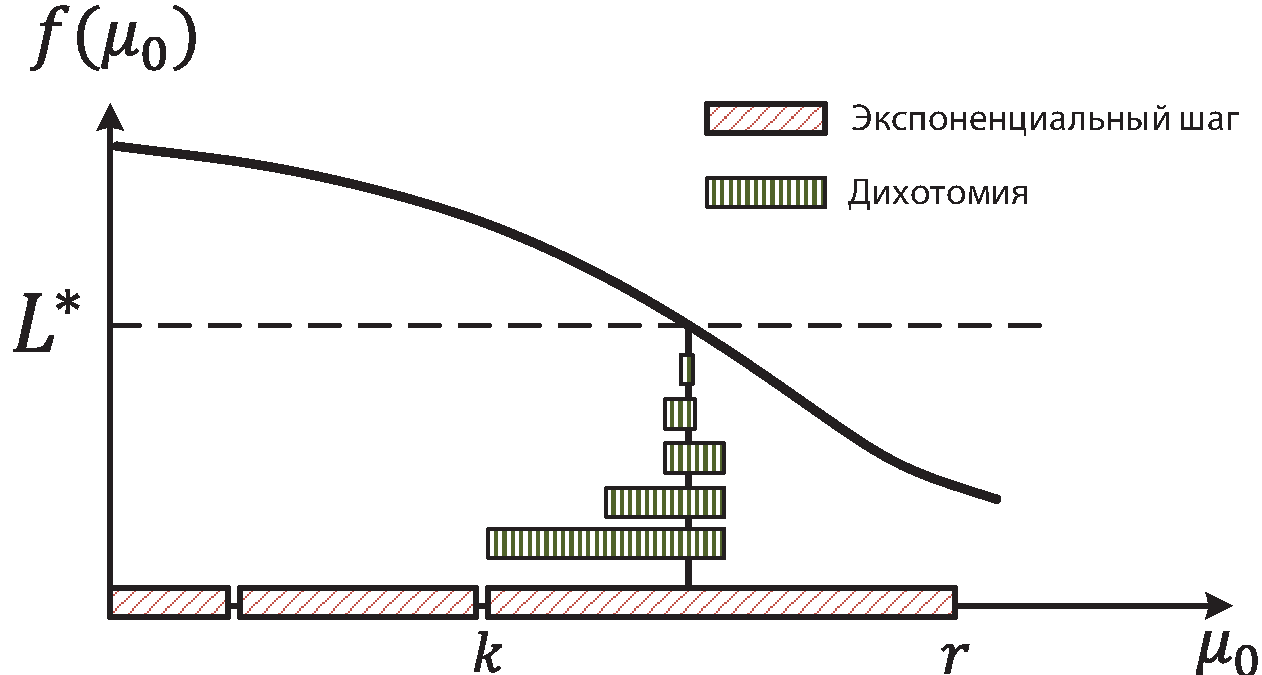
\includegraphics[width=0.7\textwidth]{Chapter4/numerical_alg.pdf}
\caption{Графическое представления алгоритма численного нахождения решения}
\label{fig:numerical_alg}
\end{center}
\end{figure}

Следующим этапом рассмотрения решения оптимизационной задачи (\ref{eq:optim_problem_bakin_lemma}) является оценка сложности полученного решения. Численный алгоритм \ref{alg:algorithm_numerical_solution} обладает логарифмической сложностью от требуемой точности нахождения решения уравнения (\ref{eq:optim_problem_bakin_lemma_solution_eq}) \cite{convex_opt, Bakin_Globecom}. На основе данного факта справедливо следующее: сложность алгоритма \ref{alg:algorithm_numerical_solution}, нахождения решения оптимизационной задачи (\ref{eq:optim_problem_bakin_lemma}), является сопоставимой со сложностью алгоритма \ref{alg:algorithm_lemma}: $O(N log_2 N), N \to \infty$ (подраздел \ref{chap3:GeneralizedFKSP}, таблица \ref{tab:nonadaptiveComplexity}).

\section{Нижняя граница отношения длительностей буферизации и просмотра при передаче адаптивных видеопотоков}
\label{chap4:LowerBoundForQ}
В подразделе \ref{chap4:AdaptiveOptimizationProblem} была предложена оптимизационная задача невыпуклого программирования (\ref{eq:optim_problem_q}), определяющая максимально возможную производительность беспроводных централизованных систем для передачи адаптивных видеопотоков. Данная оптимизационная задача учитывает два основных фактора, влияющие на качество восприятия адаптивного видео: отношение длительностей буферизации и просмотра ($q_i$) и средняя битовая скорость просмотренного видео ($\tilde{R}_i$), представленные в подразделе \ref{chap4:AdaptiveQoe}. Сложность получения решения задачи (\ref{eq:optim_problem_q}) обусловлена невыпуклостью ее ограничения, что приводит к отсутствию стандартных методов и подходов к решению. Оптимизационная задача (\ref{eq:optim_problem_q}) имеет следующий вид:

$$\begin{array}{l}
\text{ \textbf{Минимизировать:} } \frac{1}{N}\sum\limits_{i=1}^N q_i \\
\text{ \textbf{При условии:} }\\
\begin{cases}
\sum\limits_{i=1}^{N} {\left(1-\nu^R_i\nu^C_i\right)\frac{\tilde{R}_i \tilde{C}^{-1}_i }{q_i + \gamma_i}} -1 \leq 0 \\
-\frac{1}{N}\sum\limits_{i=1}^{N}\tilde{R}_i + R_{avg} \leq 0 \\
\tilde{R}_i \in \left[R_{min}, R_{max}\right], i=\overline{1,N} \\
-q_i \leq 0,\mbox{ }i=\overline{1,N} \\
\end{cases}
\end{array}.$$

Предлагаемый подход для решения задачи (\ref{eq:optim_problem_q}) состоит в разделении ее решения на два этапа.

На первом этапе будет рассмотрена промежуточная задача (\ref{eq:optim_problem_lemma_q_first}):

\begin{equation}
\begin{array}{l}
\text{ \textbf{Максимизировать:} } L = \sum\limits_{i=1}^N l_i \\
\text{ \textbf{При условии:} }\\
\begin{cases}
\sum\limits_{i=1}^{N} {l_i \tilde{R}_i - 1} \leq 0\\
-\frac{1}{N}\sum\limits_{i=1}^{N}\tilde{R}_i + R_{avg} \leq 0 \\
l_i \in \left[0, \frac{\left(1-\nu^R_i\nu^C_i\right)\tilde{C}^{-1}_i }{\gamma_i}\right] , & i=\overline{1,N} \\
\tilde{R}_i \in \left[R_{min}, R_{max}\right] , & i=\overline{1,N} \\
\end{cases}
\end{array}.
\label{eq:optim_problem_lemma_q_first}
\end{equation}

Оптимизационная задача (\ref{eq:optim_problem_lemma_q_first}) является задачей с линейной целевой функцией и одним невыпуклым ограничением квадратичного вида. Важным отличием оптимизационной задачи (\ref{eq:optim_problem_lemma_q_first}) от (\ref{eq:optim_problem_q}) состоит в виде первого ограничения: ограничение в задаче (\ref{eq:optim_problem_q}) является \textit{ограничением общего вида} (подраздел \ref{chap4:AdaptiveOptimizationProblem}), когда ограничение в задаче (\ref{eq:optim_problem_q}) является \textit{ограничением квадратичного вида}. Это небольшое отличие оптимизационных задач, имеет колоссальное влияние на методику решения. Для задач квадратичного программирования, с невыпуклым ограничением квадратичного вида существует эффективный алгоритм решения, построенный на основе метода многогранной аппроксимации (в англоязычной литературе \textit{<<polyhedral underestimating method>>}), в сочетании со стандартными численными методами решения задач выпуклого программирования \cite{Zheng2011}. Описание данного численного метода решения задач квадратичного программирования с невыпуклым квадратичным ограничением является очень громоздким и не приводится в рамках настоящей работы, так как не является результатом, полученным автором.

Оптимизационная задача (\ref{eq:optim_problem_lemma_q_first}) сохраняет все ограничения задачи (\ref{eq:optim_problem_q}), но вводит обозначение:
$$l_i = \left(1-\nu^R_i\nu^C_i\right)\frac{\tilde{C}^{-1}_i }{q_i + \gamma_i}.$$
Используя введенное обозначение, преобразуем ограничения оптимизационной задачи (\ref{eq:optim_problem_q}). Так как $q_i, i = \overline{1,N}$ может принимать значения в $[0, \infty)$, то значения $l_i, i = \overline{1,N}$ должны принимать значения в отрезке $\left[0, \frac{\left(1-\nu^R_i\nu^C_i\right)\tilde{C}^{-1}_i }{\gamma_i}\right]$, что отражено в задаче (\ref{eq:optim_problem_lemma_q_first}).

Взаимосвязь решений задач (\ref{eq:optim_problem_q}) и (\ref{eq:optim_problem_lemma_q_first}) описывается утверждением \ref{lem:q_lemma}.

\begin{lemma}
\label{lem:q_lemma}
Для оптимальных значений вектора $\left\{q^{*}_i\right\}$ задачи (\ref{eq:optim_problem_q}) и оптимального решения $L^{*}$ задачи (\ref{eq:optim_problem_lemma_q_first}) справедливо следующее неравенство:
$$\sum\limits_{i=1}^{N} {\frac{\tilde{a}_i}{q^{*}_i + \gamma_i}} \leq L^{*},$$
где $\tilde{a}_i = \left(1-\nu^R_i\nu^C_i\right)\tilde{C}^{-1}_i$.
\end{lemma}

\begin{proof}

Доказательство утверждения \ref{lem:q_lemma} построено на основе метода от противного. Предположим, что это не так, тогда надутся значения $q^*_i, i=\overline{1,N}$:
$$\sum\limits_{i=1}^{N} {\frac{\tilde{a}_i}{q^*_i + \gamma_i}} > L^{*}.$$
Следовательно, существует $l^o_i = \frac{\tilde{a}_i}{q^*_i+\gamma_i}$, $i=\overline{1,N}$, удовлетворяющие ограничениям оптимизационной задачи (\ref{eq:optim_problem_lemma_q_first}). Тогда $\sum\limits_{i=1}^{N} {l^o_i} > L^{*}$, однако, из данного соотношения следует, что значение $L^{*}$ не было решением задачи (\ref{eq:optim_problem_lemma_q_first}). Таким образом, было найдено противоречие. Настоящий факт завершает доказательство.
\end{proof}
Используя результат утверждения \ref{lem:q_lemma}, предлагается постановка оптимизационной задачи (\ref{eq:optim_problem_q}) с ослабленными ограничениями:
\begin{equation}
\nonumber
\begin{array}{l}
\text{ \textbf{Минимизировать:} } \frac{1}{N}\sum\limits_{i=1}^N q_i \\
\text{ \textbf{При условии:} }\\
\begin{cases}
\sum\limits_{i=1}^{N} {\frac{\tilde{a}_i}{q_i + \gamma_i}} - L^{*} \leq 0\\
-q_i \leq 0 , i=\overline{1,N} \\
\end{cases}
\end{array}.
\end{equation}

Данная постановка задачи повторяет оптимизационную задачу (\ref{eq:optim_problem_bakin_lemma}), представленную в подразделе \ref{chap4:KktSolution}. Обозначения, используемые в настоящей постановке и задаче (\ref{eq:optim_problem_bakin_lemma}), согласованы. Основываясь решении задачи (\ref{eq:optim_problem_bakin_lemma}), приведенному в подразделе \ref{chap4:KktSolution}, и обобщая ранее приведенные результаты, предлагается следующая теорема.

\begin{theoremapp}
\label{thr:QTheorem}
Нижняя граница для среднего значения отношений длительностей буферизации и просмотра при передаче адаптивных видеопотоков может быть вычислена алгоритмом \ref{alg:QTheoremAlgorithm}.
\end{theoremapp}

\begin{algorithm}
  \caption{: Вычисление нижней границы отношения длительностей буферизации и просмотра при передаче адаптивных видеопотоков}
	\label{alg:QTheoremAlgorithm}
  \begin{algorithmic}[1]
	 \item Вычисление $L^{*}$~--~решение оптимизационной задачи (\ref{eq:optim_problem_lemma_q_first});
	 \item Нахождение значения $\mu$ являющегося решением уравнения: $$\sum\limits_{i=1}^{N} {\frac{\tilde{a}_i}{\mathrm{max} \left(\sqrt{\mu \tilde{a}_i N}, \gamma_i\right)}} - L^{*} = 0;$$
	\item Подстановка значения $\mu$, полученного на предыдущем шаге, в выражение для вычисления нижней границы:
	$$Q =
	\begin{cases}
	0, & \text{если} \sum\limits_{i=1}^{N} {\left(\frac{\tilde{a}_i}{\gamma_i}\right)} \leq L^{*}\\
	\frac{1}{N} \sum\limits_{i=1}^{N} {\mathrm{max} \left(\sqrt{\mu \tilde{a}_i N}-\gamma_i, 0\right)}, & \mathrm{иначе} \\
	\end{cases}.$$
  \end{algorithmic}
\end{algorithm}

Завершающим этапом настоящего подраздела является анализ сложности вычисления нижней границы отношения длительностей буферизации к длительности просмотра при передаче адаптивных видеопотоков. В алгоритме \ref{alg:QTheoremAlgorithm} наибольшей вычислительной сложностью обладает шаг 1: поиск решения оптимизационной задачи (\ref{eq:optim_problem_lemma_q_first}) с использованием численных методов нахождения минимума целевой функции при ограничениях типа неравенства. Сложность подобных методов и их сравнение с возможными аналогами было приведено в таблице \ref{tab:nonadaptiveComplexity} подраздел \ref{chap3:GeneralizedFKSP}.

Таким образом, алгоритм \ref{alg:QTheoremAlgorithm} обладает высокой вычислительной сложностью и не может быть реализован в реальном масштабе времени при организации управления распределением ресурсов беспроводного канала на базовой станции. Однако, данное свойство не снижает значимости полученного результата для аналитической оценки производительности беспроводных централизованных сетей при передаче адаптивного видео. Настоящий результат может быть использован при планировании сетей беспроводной связи (расположение и характеристики устанавливаемых базовых станций) и создания требований к алгоритмам планирования ресурсов беспроводного канала для существующих и будущих стандартов беспроводной связи.

\section{Численный пример}
\label{chap4:NumericalExample}

Настоящий подраздел демонстрирует результаты сравнения нижней границы для отношения длительностей буферизации и просмотра, представленной в подразделе \ref{chap4:LowerBoundForQ}, с известными алгоритмами планирования (подраздел~\ref{chap2:Scheduler}).

Демонстрация результатов настоящего раздела производится в соответствии с подразделом \ref{chap3:NumericalExample}. Рассматривается работа одной соты, где пользователи находятся на одной линии по удалению от базовой станции. Состояние беспроводного канала изменяется во времени, так как в моделировании используется модель радиоканала с плоскими замираниями.

На рисунке \ref{fig:Q_PLOT} представлено сравнение производительности известных алгоритмов планирования (\textit{Round Robin} и \textit{Proportional Fair}) с нижней границей при зафиксированном числе абонентов в соте, равном 10 пользователям. По оси абсцисс отложена требуемая средняя скорость просматриваемого видеопотока в соте, а по оси ординат значение критерия качества восприятия $Q$. Заштрихованная область под кривой, определяющей нижнюю границу, характеризует область, значения которой недостижимы для всевозможных алгоритмов планирования, удовлетворяющих введенным допущениям в подразделе \ref{chap2:Assumptions}, например, не существует алгоритмов планирования и адаптации видеоряда, обеспечивающих значения критерия качества восприятия $Q$ равном $0.05$ при средней битовой скорости просматриваемых видеопотоков равной $3.75$ Мбит/с, когда в соте находится 10 абонентов. Найденная нижняя граница для адаптивных видеопотоков сравнивается с уже известной нижней границей для неадаптивных, представленной в работе \cite{Bakin_Globecom}. При моделировании и расчете характеристик для неадаптивного видео предполагалось, что все пользователи просматривают видео с битвой скоростью равной $R_{avg}$.


Из результатов, представленных на рисунке \ref{fig:Q_PLOT}, следует:
\begin{itemize}
	\item Использование адаптивной технологии передачи видеоданных позволяет достичь большей производительности беспроводной централизованной сети передачи информации.
	\item Планировщик \textit{Proportional Fair} обладает большей производительностью в сравнении с алгоритмом \textit{Round Robin}, и демонстрирует производительность близкую к нижней границе по критерию качества $Q$.
\end{itemize}


\begin{figure}[htbp]
\begin{center}
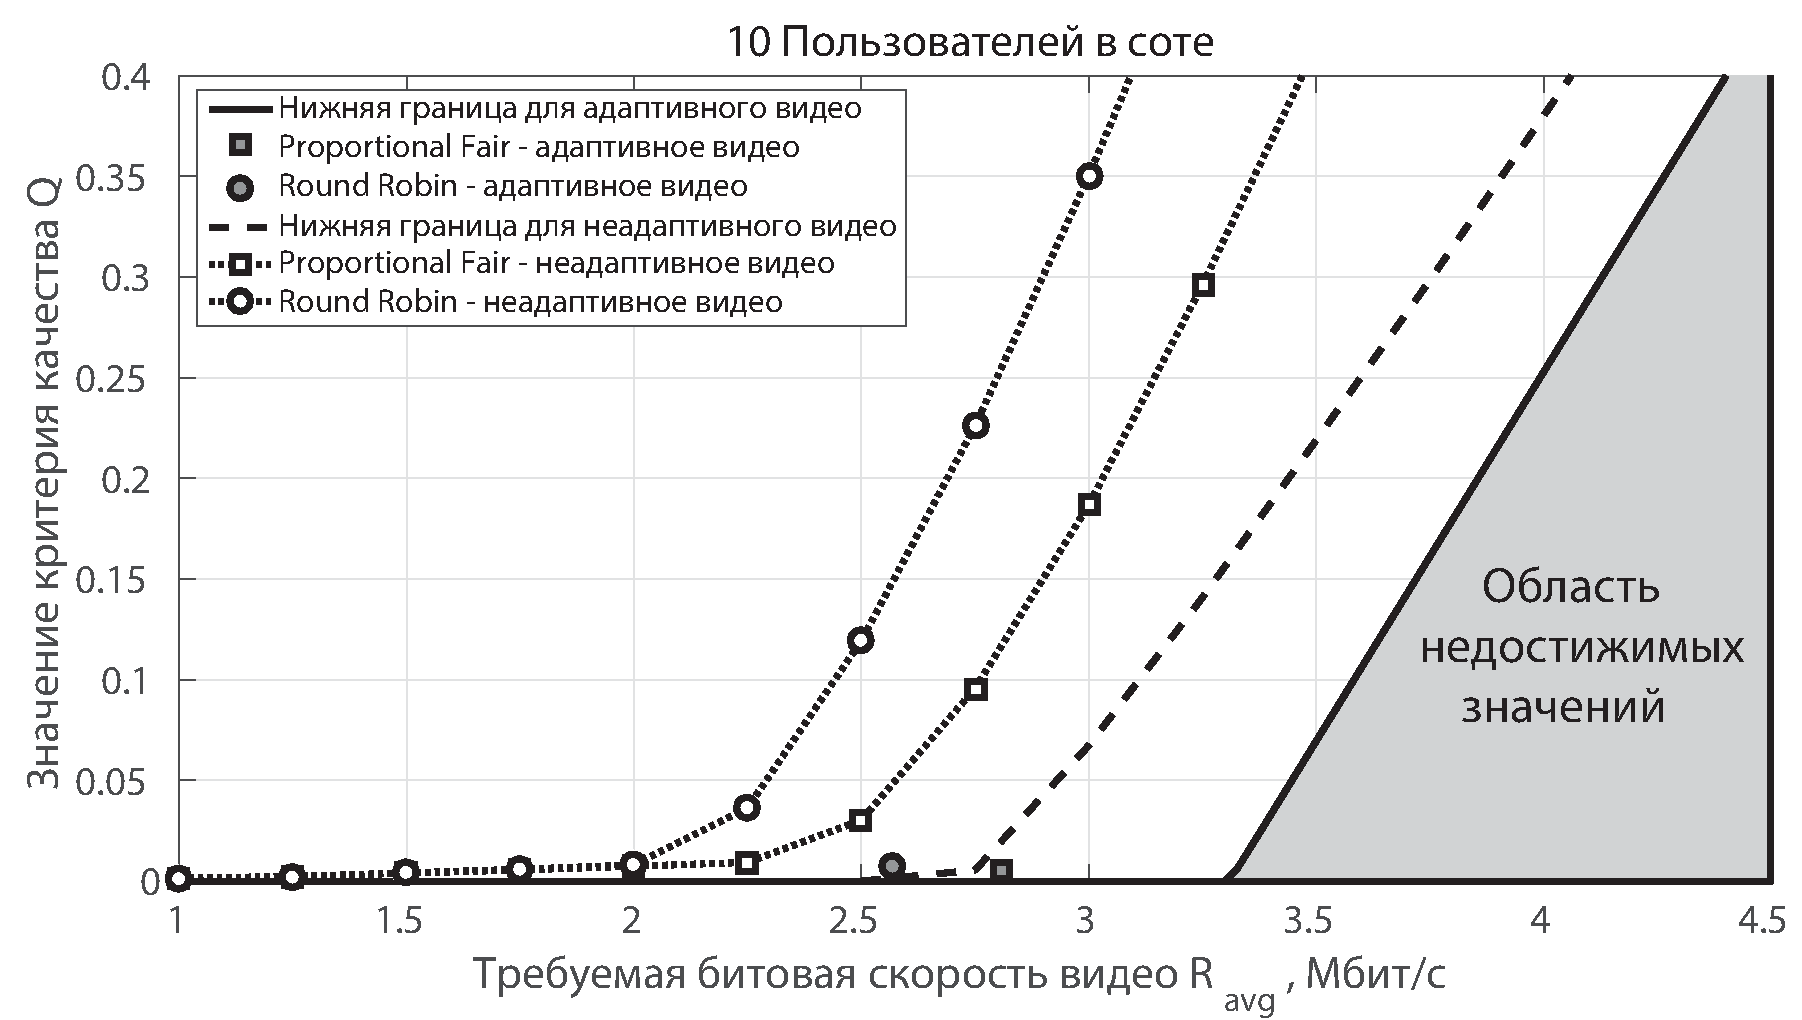
\includegraphics[width=\textwidth]{/Chapter4/10_Users_v2.pdf}
\caption{Сравнение производительности известных алгоритмов планирования при передаче адаптивного видео с нижней границей}
\label{fig:Q_PLOT}
\end{center}
\end{figure}

На рисунке \ref{fig:Users_cmp} представлено сравнение нижних границ для критерия $Q$ при наличии различного числа абонентов в соте. С ростом числа абонентов при заданном уровне значений критерия $Q$ система переходит в состояние перегрузки (определение \ref{def:Congestion}) при меньшем значении требуемой средней битовой скорости видеопотоков в соте.

\begin{figure}[htbp]
\begin{center}
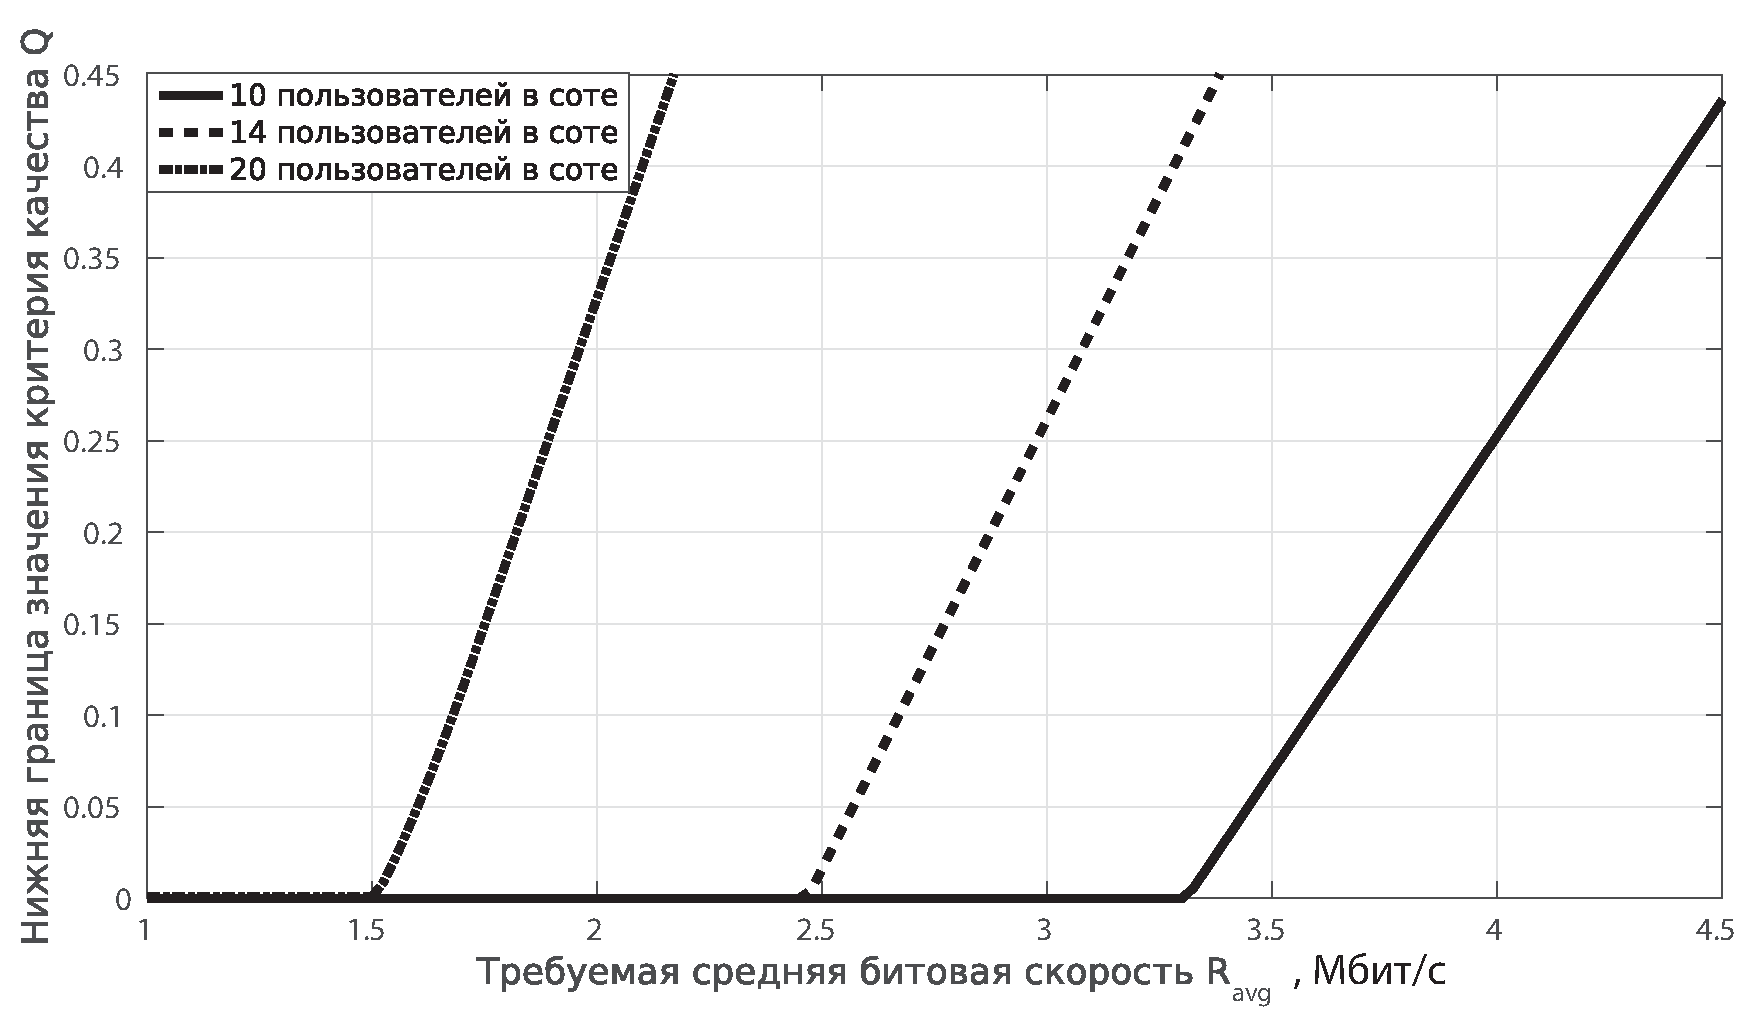
\includegraphics[width=\textwidth]{/Chapter4/Users_cmp.pdf}
\caption{Нижняя граница для критерия $Q$ при различном числе абонентов в соте}
\label{fig:Users_cmp}
\end{center}
\end{figure}

Введем определение емкости соты:
\begin{definition}
\label{def:Capacity}
    \emph{Емкость соты}~--~число пользователей в соте, при котом значение критерия $Q$ равняется некоторой заданной величине.
\end{definition}
Определение \ref{def:Capacity} взаимосвязано с определеним перегрузки следующим образом: определение перегрузки задает границу значения критерия качества восприятия, при котором система перестает поддерживать требуемый уровень качества обслуживания. В свою очередь определение емкости соты определяет максимальное число пользователей, при котором система еще не перешла в состояние перегрузки.

Рисунок \ref{fig:capacity} иллюстрирует максимально возможную емкость соты для рассматриваемого сценария при значении критерия восприятия $Q$ равном $0.01$, $0.05$ и $0.1$ в зависимости от требуемой битовой скорости просматриваемых видеопотоков. Возможно отметить, что наибольшая емкость соты достигается при больших значениях критерия качетсва $Q$.

\begin{figure}[htbp]
\begin{center}
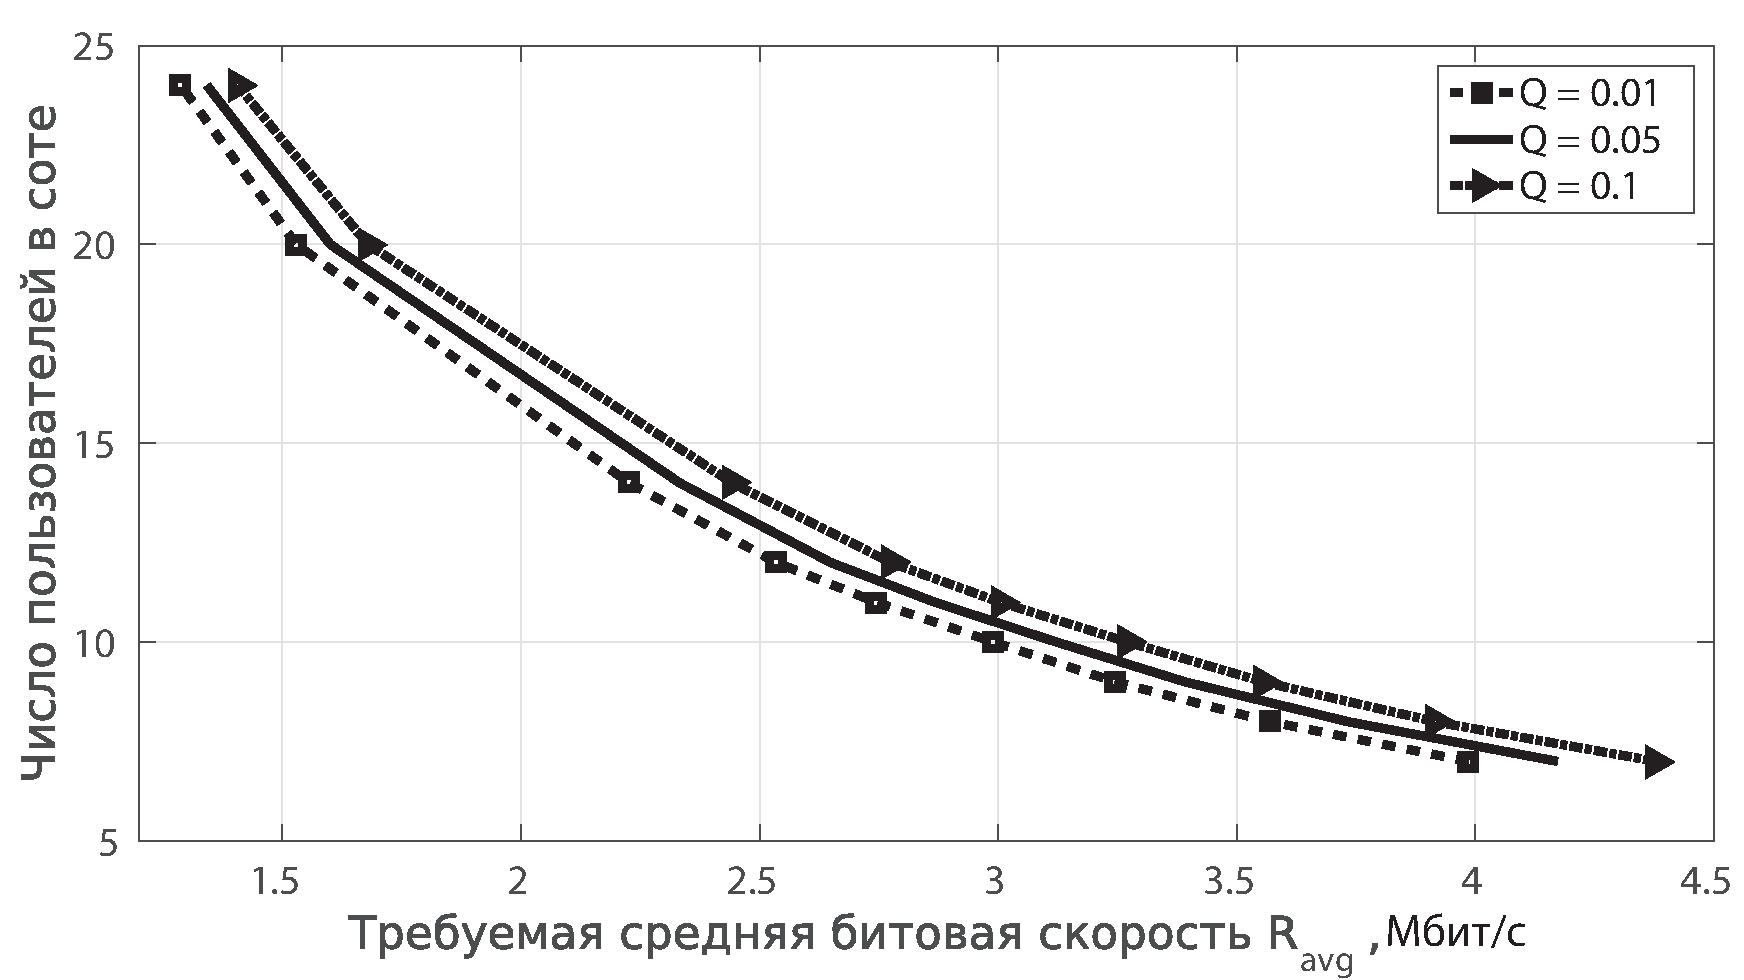
\includegraphics[width=\textwidth]{/Chapter4/capacity.pdf}
\caption{Максимальная емкость соты для различных значений критерия качества $Q$}
\label{fig:capacity}
\end{center}
\end{figure}

\section{Выводы по разделу}

В настоящем разделе была рассмотрена передача адаптивных видеопотоков по протоколу HTTP в беспроводных централизованных сетях связи. В начале раздела был предложен критерий качества восприятия адаптивного видео, учитывающий два основных фактора: длительность буферизации и битовая скорость просматриваемого видеопотока. На основе данного критерия была сформулирована оптимизационная задача невыпуклого программирования, определяющая максимально возможную производительность систем передачи информации для введенного критерия. Для поставленной оптимизационной задачи была найдена нижняя граница по всевозможным алгоритмам планирования распределения ресурсов беспроводного канала и адаптации видеопотока, удовлетворяющих допущениям, введенным в подразделе \ref{chap2:Assumptions}. В заключении раздела была продемонстрировано сравнение производительности существующих алгоритмов планирования с найденной нижней границей, и определена максимально возможная емкость соты для рассматриваемого сценария при передаче адаптивных видеопотоков.

В качестве результатов настоящего раздела могут быть выделены следующие:
\begin{itemize}
	\item Предложен критерий качества восприятия адаптивного видео: отношение длительностей буферизации и просмотра при ограничении снизу на среднее значение битовой скорости просматриваемого видеопотока (подраздел \ref{chap4:AdaptiveQoe});
	\item Для предложенного критерия произведена постановка оптимизационной задачи невыпуклого программирования. Для данной постановки найдена нижняя граница для введенного критерия по всевозможным алгоритмам планирования и адаптации видеопотока, удовлетворяющих введенным допущениям в подразделе \ref{chap2:Assumptions}, с использованием двуступенчатой оптимизации (подразделы \ref{chap4:AdaptiveOptimizationProblem}, \ref{chap4:KktSolution} и \ref{chap4:LowerBoundForQ});
	\item Произведена демонстрация производительности существующих алгоритмов планирования в сравнении с найденной нижней границей и определена максимально возможная емкость соты для рассматриваемого сценария (подраздел \ref{chap4:NumericalExample}).
\end{itemize}

Настоящий раздел является заключительным в диссертационном исследовании и, для демонстрации общей картины проделанной работы, в приложении \ref{AppС} представлен граф основных зависимостей между подразделами (рисунок \ref{fig:graph_horizontal.pdf}). Нумерация узлов графа соответствует нумерации подразделов, направленные ребра (сплошные линии) обозначают прямые ссылки между подразделами (например, подраздел \ref{chap3:NonAdaptiveOptimizationProblem} ссылается на подразделы \ref{chap2:Assumptions} и \ref{chap2:InterrelationVideoParams}), пунктирные линии обозначают логическое соединение материалов подразделов.

Возможно отметить, что опорными подразделами настоящей работы являются \ref{chap2:Assumptions} и \ref{chap2:InterrelationVideoParams}, представляющие систему допущений и основополагающую взаимосвязь между характеристиками сети передачи информации и воспроизведением видеоряда соответственно. Основные результаты работы, представленные в подразделах \ref{chap2:InterrelationVideoParams}, \ref{chap3:LowerBoundForG} и \ref{chap4:LowerBoundForQ}, и их демонстрации \ref{chap3:NumericalExample} и \ref{chap4:NumericalExample}, непосредственно опираются на систему допущений (подраздел \ref{chap2:Assumptions}). Материалы подраздела \ref{chap2:Assumptions} сформированы на основе анализа передачи видео по протоколу HTTP (раздел \ref{chap1}) и современных беспроводных централизованных телекоммуникационных систем (подразделы \ref{chap2:WirelessSystemStructure}, \ref{chap2:RadioChannel} и \ref{chap2:Scheduler}).

Важным моментом проведенного исследования является связь между системой передачи видеоданных и замкнутой системой массового обслуживания с конечным числом абонентов (подраздел \ref{chap2:QueuningNetwork}). Из материалов подраздела \ref{chap2:QueuningNetwork} следует, что исследуемая система является обобщением замкнутой СМО с конечным числом абонентов, в которой каждая генерируемая заявка уникальна и длительности пауз между их отправками не являются экспоненциальными случайными величинами, а интенсивность обслуживания изменяется во времени и зависит от характеристик всего множества заявок, находящихся в буфере на обслуживающем устройстве. Настоящее диссертационное исследование предлагает новые аналитические результаты для подобных систем массового обслуживания.           % Раздел 4
\chapter*{ЗАКЛЮЧЕНИЕ}						% Заголовок
\addcontentsline{toc}{chapter}{ЗАКЛЮЧЕНИЕ}	% Добавляем его в оглавление

%% Согласно ГОСТ Р 7.0.11-2011:
%% 5.3.3 В заключении диссертации излагают итоги выполненного исследования, рекомендации, перспективы дальнейшей разработки темы.
%% 9.2.3 В заключении автореферата диссертации излагают итоги данного исследования, рекомендации и перспективы дальнейшей разработки темы.
%% Поэтому имеет смысл сделать эту часть общей и загрузить из одного файла в автореферат и в диссертацию:

В диссертационной работе рассмотрена передача видеоданных по протоколу HTTP в беспроводных централизованных системах связи. Основное внимание уделено аналитическим исследованиям макисмально возможной производительности подобных систем при доминировании передачи видео.

Основные результаты работы заключаются в следующем.
%% Согласно ГОСТ Р 7.0.11-2011:
%% 5.3.3 В заключении диссертации излагают итоги выполненного исследования, рекомендации, перспективы дальнейшей разработки темы.
%% 9.2.3 В заключении автореферата диссертации излагают итоги данного исследования, рекомендации и перспективы дальнейшей разработки темы.
\begin{enumerate}
    \item Предложена модель беспроводной централизованной сети связи при передаче видеоданных по протоколу HTTP. Найдена взаимосвязь между объективными характеристиками сети и качеством воспроизведения видео. Предложенная модель и найденная взаимосвязь позволяют производить аналитические исследования производительности беспроводных централизованных сетей при доминировании передачи видеоданных.
    \item Предложены алгоритмы вычисления граничных значений максимально возможной производительности беспроводных централизованных сетей для следующих критериев качества восприятия:
    \begin{itemize}
	    \item Нормированное отношение длительности буферизации к просмотру при передаче неадаптивных видеопоследовательностей;
	    \item Отношение длительности буферизации к просмотру с учетом средней битовой скорости видео при передаче адаптивного видео.
    \end{itemize}
    Полученные результаты могут быть использованы в качестве опорных значений при разработке новых алгоритмов планирования, учитывающие тип передаваемого трафика и требования к его обслуживанию, для существующих и последующих стандартов беспроводной связи.
    \item Предложен алгоритм планирования распределения ресурсов беспроводного канала, позволяющий минимизировать нормированное отношение длительности буферизации к просмотру при передаче неадаптивного видео. Предложенный алгоритм позволяет увеличить емкость соты на $7-14\%$ в сравнении с известными решениями и демонстрирует производительность близкую к найденной аналитической границе.
\end{enumerate}

      % Заключение
\clearpage                                  % В том числе гарантирует, что список литературы в оглавлении будет с правильным номером страницы
\phantomsection
\addcontentsline{toc}{chapter}{\bibname}	% Добавляем список литературы в оглавление
%\hypersetup{ urlcolor=black }               % Ссылки делаем чёрными
%\providecommand*{\BibDash}{}                % В стилях ugost2008 отключаем использование тире как разделителя 
\urlstyle{rm}                               % ссылки URL обычным шрифтом
\insertbibliofull                           % Подключаем Bib-базы
\urlstyle{tt}                               % возвращаем установки шрифта ссылок URL
%\hypersetup{ urlcolor={urlcolor} }          % Восстанавливаем цвет ссылок      % Список литературы
\clearpage
\phantomsection
\addcontentsline{toc}{chapter}{\listfigurename}
\listoffigures									% Список изображений


%%% Список таблиц %%%
% (ГОСТ Р 7.0.11-2011, 5.3.10)
\clearpage
\phantomsection
\addcontentsline{toc}{chapter}{\listtablename}
\listoftables									% Список таблиц
\newpage           % Списки таблиц и изображений (иллюстративный материал)
\appendix
%% Правка оформления ссылок на приложения:
%http://tex.stackexchange.com/questions/56839/chaptername-is-used-even-for-appendix-chapters-in-toc
%http://tex.stackexchange.com/questions/59349/table-of-contents-with-chapter-and-appendix
%% требует двойной компиляции
\addtocontents{toc}{\def\protect\cftchappresnum{\MakeUppercase{\appendixname{}} }%
\setlength{\cftchapnumwidth}{\widthof{\cftchapfont\MakeUppercase{\appendixname~Б}\cftchapaftersnum}}%
}
%% Оформление заголовков приложений ближе к ГОСТ:
\sectionformat{\chapter}[display]{% Параметры заголовков разделов в тексте
    label=\MakeUppercase{\appendixname}\ \thechapter,% (ГОСТ Р 2.105, 4.3.6)
    labelsep=20pt,
}
%%\renewcommand{\chaptername}{ПРИЛОЖЕНИЕ}
\renewcommand\thechapter{\Asbuk{chapter}} % Чтобы приложения русскими буквами нумеровались
\begin{landscape}
\chapter{АППРОКСИМАЦИИ ФУНКЦИИ MOS ДЛЯ ПЕРЕДАЧИ ВИДЕОДАННЫХ}
\label{AppA}
   \begin{longtable}[H]{| C{10cm} | C{13cm} | C{2cm} |}
    \caption{Аппроксимации функции MOS для передачи видеоданных}\label{tab:appraximations} \\
    \hline
    Формула & Описание & Источник \\
    \hline
    \multicolumn{3}{|c|}{Процент замирания воспроизведения потока (Stalling, Rebuffering Percentage)}\\
    \hline
    ${{g}_{i}}=\underset{t~\to \infty }{\mathop{\lim }}\,\frac{r{{b}_{i}}\left( t \right)}{r{{b}_{i}}\left( t \right)+{{d}_{i}}\left( t \right)}$\newline
$Minimize:\underset{i}{\mathop \sum }\,{{g}_{i}}$  & $g_i$~--~процент времени, когда пользователь наблюдал прерывание воспроизведения потока; \newline $rb_i(t)$~--~длительность замираний воспроизведения потока за время $t$; \newline $d_i(t)$~--~длительность просмотренной последовательности за время $t$. & \cite{QoE_Ozgur,past_tur}\\
    \hline
    ${{q}_{i}}=\underset{t~\to \infty }{\mathop{\text{lim}}}\,\frac{{{w}_{i}}\left( t \right)}{{{d}_{i}}\left( t \right)}$ \newline
$Minimize:\underset{i}{\mathop \sum }\,{{q}_{i}}$  & $w_i(t)$~--~длительность ожидания в течении времени t, учитывающее начальные буферизации и прерывания воспроизведения потока. & \cite{Bakin_Globecom}\\
    \hline
    \multicolumn{3}{|c|}{Взвешенные суммы характеристик воспроизведения}\\
    \hline
    $MO{{S}_{i}}={{f}_{RATE}}\left( {{R}_{i}} \right)$\newline $Maximize:\sum\limits_{i}{MO{{S}_{i}}}$ & $R_i(t)$~--~битовая скорость просматриваемого потока. & \cite{Essaili_Rate} \\
    \hline
    ${{f}_{i}}=~{{k}_{1}}\ln {{R}_{i}}-{{k}_{2}}\frac{r{{b}_{i}}\left( t \right)}{{{d}_{i}}\left( t \right)}$\newline $Maximize:\underset{i}{\mathop \sum }\,{{f}_{i}}$ & $R_i(t)$~--~битовая скорость просматриваемого потока;\newline $k_1,k_2$~--~весовые коэффициенты приоритета функции от битовой скорости и замираний воспроизведения соответственно, причем $k_1 << k_2$. & \cite{Suai2015} \\
    \hline
    $Minimize:W\lambda -~\theta ~$ & $\lambda$~--~средний процент времени прерывания воспроизведения по всем пользователям;\newline $\theta$~--~среднее значение скорости битовой репрезентации по всем пользователям; \newline $W$~--~весовой коэффициент приоритета прерывания воспроизведения, сравним со значением $\theta$.& \cite{7179392} \\
    \hline
    $Qo{{E}_{i}}\left[ t \right]={{W}_{1}}$\newline$\log ({{R}_{i}}\left[ t \right]~-{{W}_{2}}{{\left( Bu{{f}_{i}}\left[ t \right]-Bu{{f}_{thr}} \right)}^{2}}$\newline$-{{W}_{3}}{{\left( {{R}_{i}}\left[ t \right]-{{R}_{i}}\left[ t-1 \right] \right)}^{2}})$ \newline $Maximize:\underset{i}{\mathop \sum }\,Qo{{E}_{i}}\left[ t \right]$ & $W_1, W_2,W_3$~--~весовые коэффициенты;\newline $R_i[t]$~--~битовая скорость в момент времени $t$;\newline $Buf_i[t]$~--~уровень буфера в момент времени $t$;\newline $Buf_{thr}$~--~ пороговое значение уровня буфера. & \cite{widash}  \\
    \hline
    $MO{{S}_{i}}=\frac{{{a}_{1}}+{{a}_{2}}Fr{{R}_{i}}+{{a}_{3}}\log \left( R_{i}^{TCP} \right)}{1+{{a}_{4}}P{{L}_{i}}+{{a}_{5}}{{\left( P{{L}_{i}} \right)}^{2}}}$\newline$Maximize:\sum\limits_{i}{MO{{S}_{i}}}$ & $a_j$~--~коэффициенты, зависящие от характеристик просматриваемого контента;\newline $FrR_i$~--~частота кадров потока; $R_{i}^{TCP}$~--~скорость получения информации;\newline $P{{L}_{i}}$~--~вероятность потери пакета. & \cite{5508802} \\
    \hline
    $MO{{S}_{i}}=\frac{b-a}{1+{{c}_{0}}{{\left( R_{i}^{TCP} \right)}^{-c1}}{{\left( {{c}_{2}} \right)}^{SU{{D}_{i}}}}}+a$\newline$Maximize:\underset{i}{\mathop \sum }\,MO{{S}_{i}}$ & $a,b$~--~нормирующие константы;\newline $c_j$~--~константы, подобранные в ходе эксперимента;\newline $SU{{D}_{i}}$~--~длительность ожидания начала воспроизведения. & \cite{6825149,6883466} \\
    \hline
    $\left\{ \begin{matrix}
   MO{{S}_{Res}}\left( Res{{l}_{i}} \right)=1.475\log \left( Res{{l}_{i}} \right)-6.15  \\
   MO{{S}_{Reb}}\left( RebRat{{e}_{i}} \right)=0.738~{{e}^{-RebRat{{e}_{i}}}}  \\
   MO{{S}_{SUD}}\left( SU{{D}_{i}} \right)=-0.02~SU{{D}_{i}}+2.53  \\
\end{matrix} \right.$\newline$MO{{S}_{i}}=0.174~MO{{S}_{Res}}\left( Res{{l}_{i}} \right)MO{{S}_{Reb}}{{\left( RebRate \right)}_{i}}\cdot$\newline$\cdot MO{{S}_{SUD}}\left( SU{{D}_{i}} \right)$\newline$Maximize:\sum\limits_{i}{MO{{S}_{i}}}$ & $Res{{l}_{i}}$~--~разрешение репрезентации;\newline$RebRate_i$~--~отношение времени просмотра к длительности опустошения буфера. & \cite{Chen_Chang_Wei} \\
    \hline

\end{longtable}
\end{landscape}
\chapter{ПАРАМЕТРЫ МОДЕЛИРОВАНИЯ}
\label{AppB}

\begin{longtable}[H]{| C{10cm} | C{7cm} |}
    \caption{Параметры моделирования}\label{tab:SimParams} \\
		\hline
 		\textbf{Название параметра} & \textbf{Значение} \\
 		\hline
 		\multicolumn{2}{|c|}{\textbf{Общие положения}} \\
		\hline
		Максимальная удаленность пользователей от базовой станции $X_{max}$ & 700 м \\
		\hline
		Типы трафика & Только видео \\
		\hline
		Длительность моделирования & 360000 с \\
		\hline
		Длительность интервала планирования & 1 мс \\
		\hline

		\multicolumn{2}{|c|}{\textbf{Беспроводной канал}} \\
		\hline
		Модель затухания распространения сигнала & Окамура-Хата \\
		\hline
		Окружение & Городская застройка \\
		\hline
		Тип города & Большой город \\
		\hline
		Мощность передатчика базовой станции & 44 дБм \\
		\hline
		Мощность передатчика пользовательского устройства & 23 дБм \\
		\hline
		Коэффициент усиления антенны базовой станции и пользовательского устройства & 10 дБ \\
		\hline
		Несущая частота & 2 ГГц \\
		\hline
		Ширина полосы передачи & 10 МГц \\
		\hline
		Модель ошибки при передаче данных & Отсутствует \\
		\hline

		\multicolumn{2}{|c|}{\textbf{Плоские замирания}} \\
		\hline
		Модель & Extended Pedestrian A (EPA) \\
		\hline
		Движение окружения  & 3 км/ч \\
		\hline
		Длительность генерируемой последовательности & 10 с \\
		\hline
		Несущая частота & 2 ГГц \\
		\hline

		\multicolumn{2}{|c|}{\textbf{TCP протокол}} \\
		\hline
		Стандарт & TCP NewReno \\
		\hline
		Размер фрагментации пакета  & 1440 Б \\
		\hline
		Минимальное значения таймаута & 1 с \\
		\hline
		Начальный размер окна  & 4320 Б \\
		\hline
		Ограничение начального роста окна быстрого старта & Неограничен \\
		\hline
		Размер буфера на приемной и передающей стороне  & 6 МБ \\
		\hline

		\multicolumn{2}{|c|}{\textbf{Алгоритм планирования для неадаптивных видеопотоков}} \\
		\hline
		Интервал усреднения оценки скорости передачи информации ($\bar{w}_{S}$) & 1000 мс \\
		\hline
		Интервал усреднения оценки максимальной пропускной способности канала ($\bar{w}_{C}$) & 1000 мс \\
		\hline
		Минимальная гарантированная скорость получения информации ($S^{min}$) & 100 Кб/с \\
		\hline

		\multicolumn{2}{|c|}{\textbf{Видео контент}} \\
		\hline
		Длительность видео & 300 с \\
		\hline
		Битовые скорости потока неадаптивных видеопоследовательностей & 1 Мбит/с \\
		\hline
		Битовые скорости потока адаптивных видеопоследовательностей & [1, 4.5] Мбит/с \\
		\hline

		\multicolumn{2}{|c|}{\textbf{Видеоплеер}} \\
		\hline
		Длительность сегмента видеоданных & 2 с \\
		\hline
		Размер начальной буферизации & 4 с \\
		\hline
		Максимальный размер буфера & 10 с \\
		\hline
		Адаптация видеопотока & Соответствует параметрам, представленным в таблице \ref{tab:DashJSParams} \\
		\hline

		\multicolumn{2}{|c|}{\textbf{Поведение пользователя}} \\
		\hline
		Начальная задержка при заказе видео & Равномерная случайная величина в отрезке [1, 60] с \\
		\hline
		Пауза между просмотрами видео & Усеченная экспоненциальная случайная величина в отрезке [15, 45] с со средним значением 30 с\\
		\hline
\end{longtable}
\begin{landscape}
\chapter{ГРАФИЧЕСКОЕ ПРЕДСТАВЛЕНИЕ ЗАВИСИМОСТЕЙ РАЗДЕЛОВ}
\label{AppС}
\begin{figure}[H]
\begin{center}
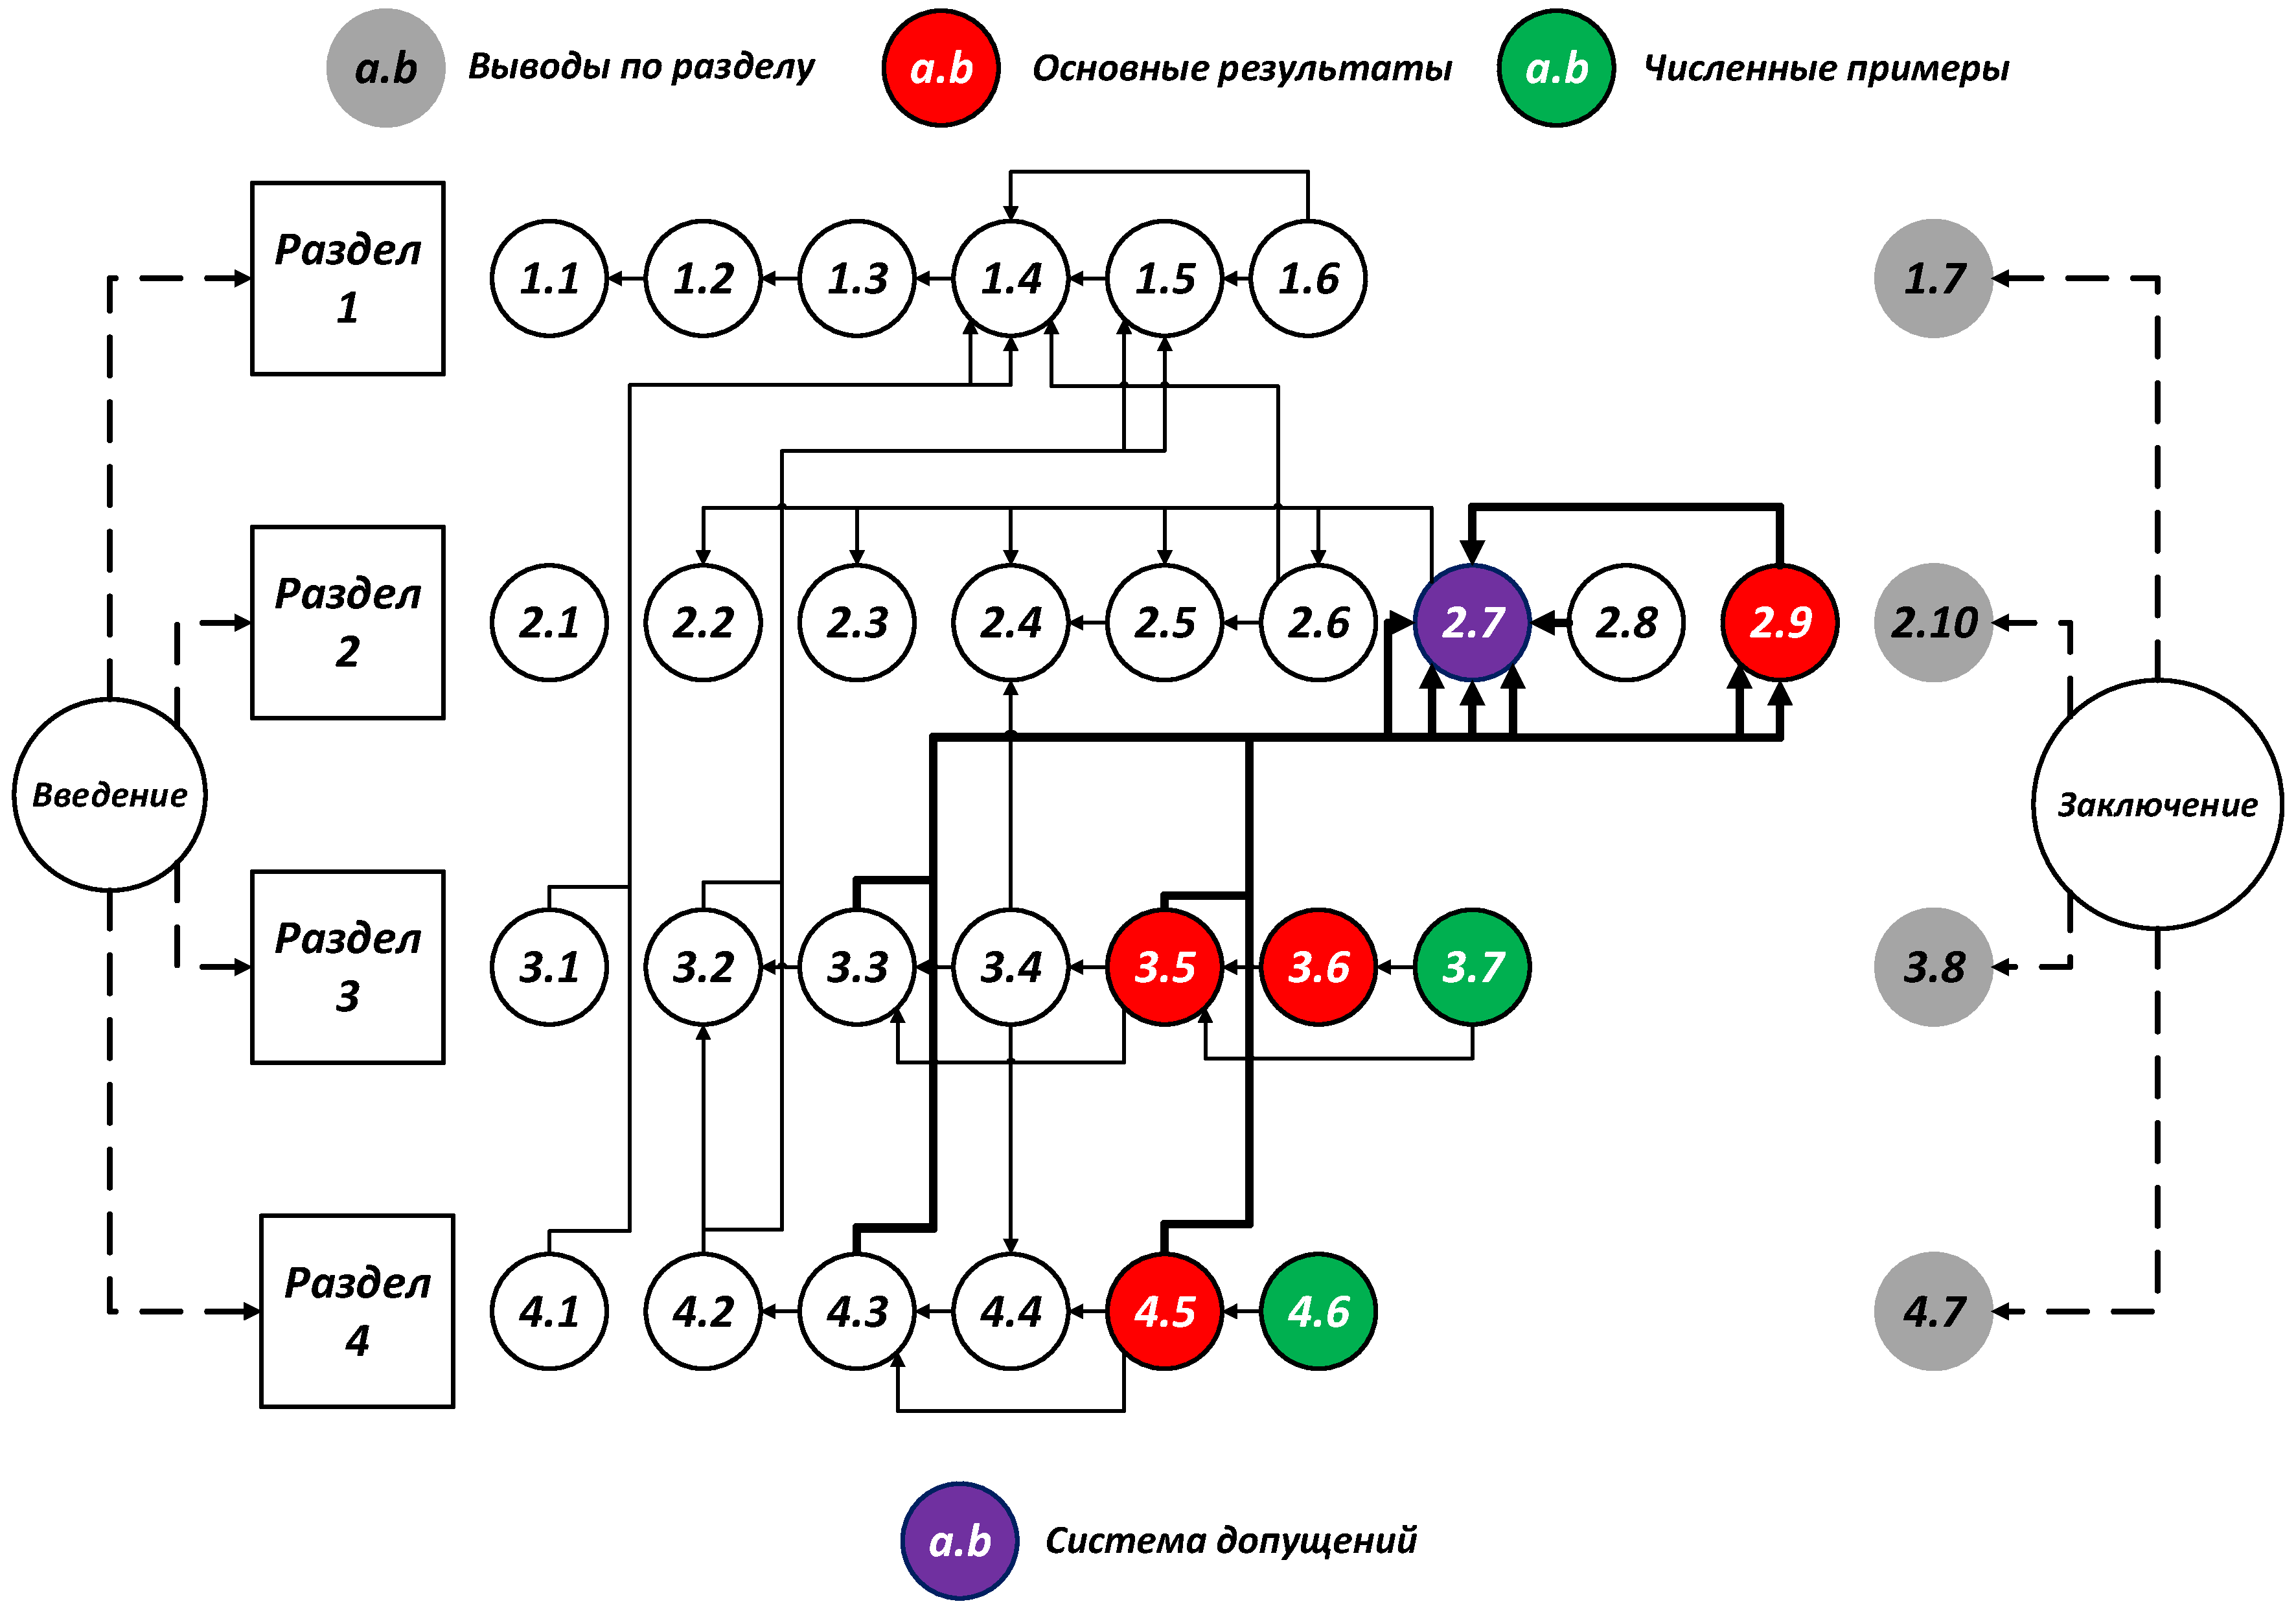
\includegraphics[width=1.2\textwidth,height=0.7\textheight]{graph_horizontal.pdf}
\caption{Графическое представление зависимостей подразделов в диссертационном исследовании}
\label{fig:graph_horizontal.pdf}
\end{center}
\end{figure}
\end{landscape}
\chapter{АКТЫ О ВНЕДРЕНИИ}
\label{AppD}
\begin{center}
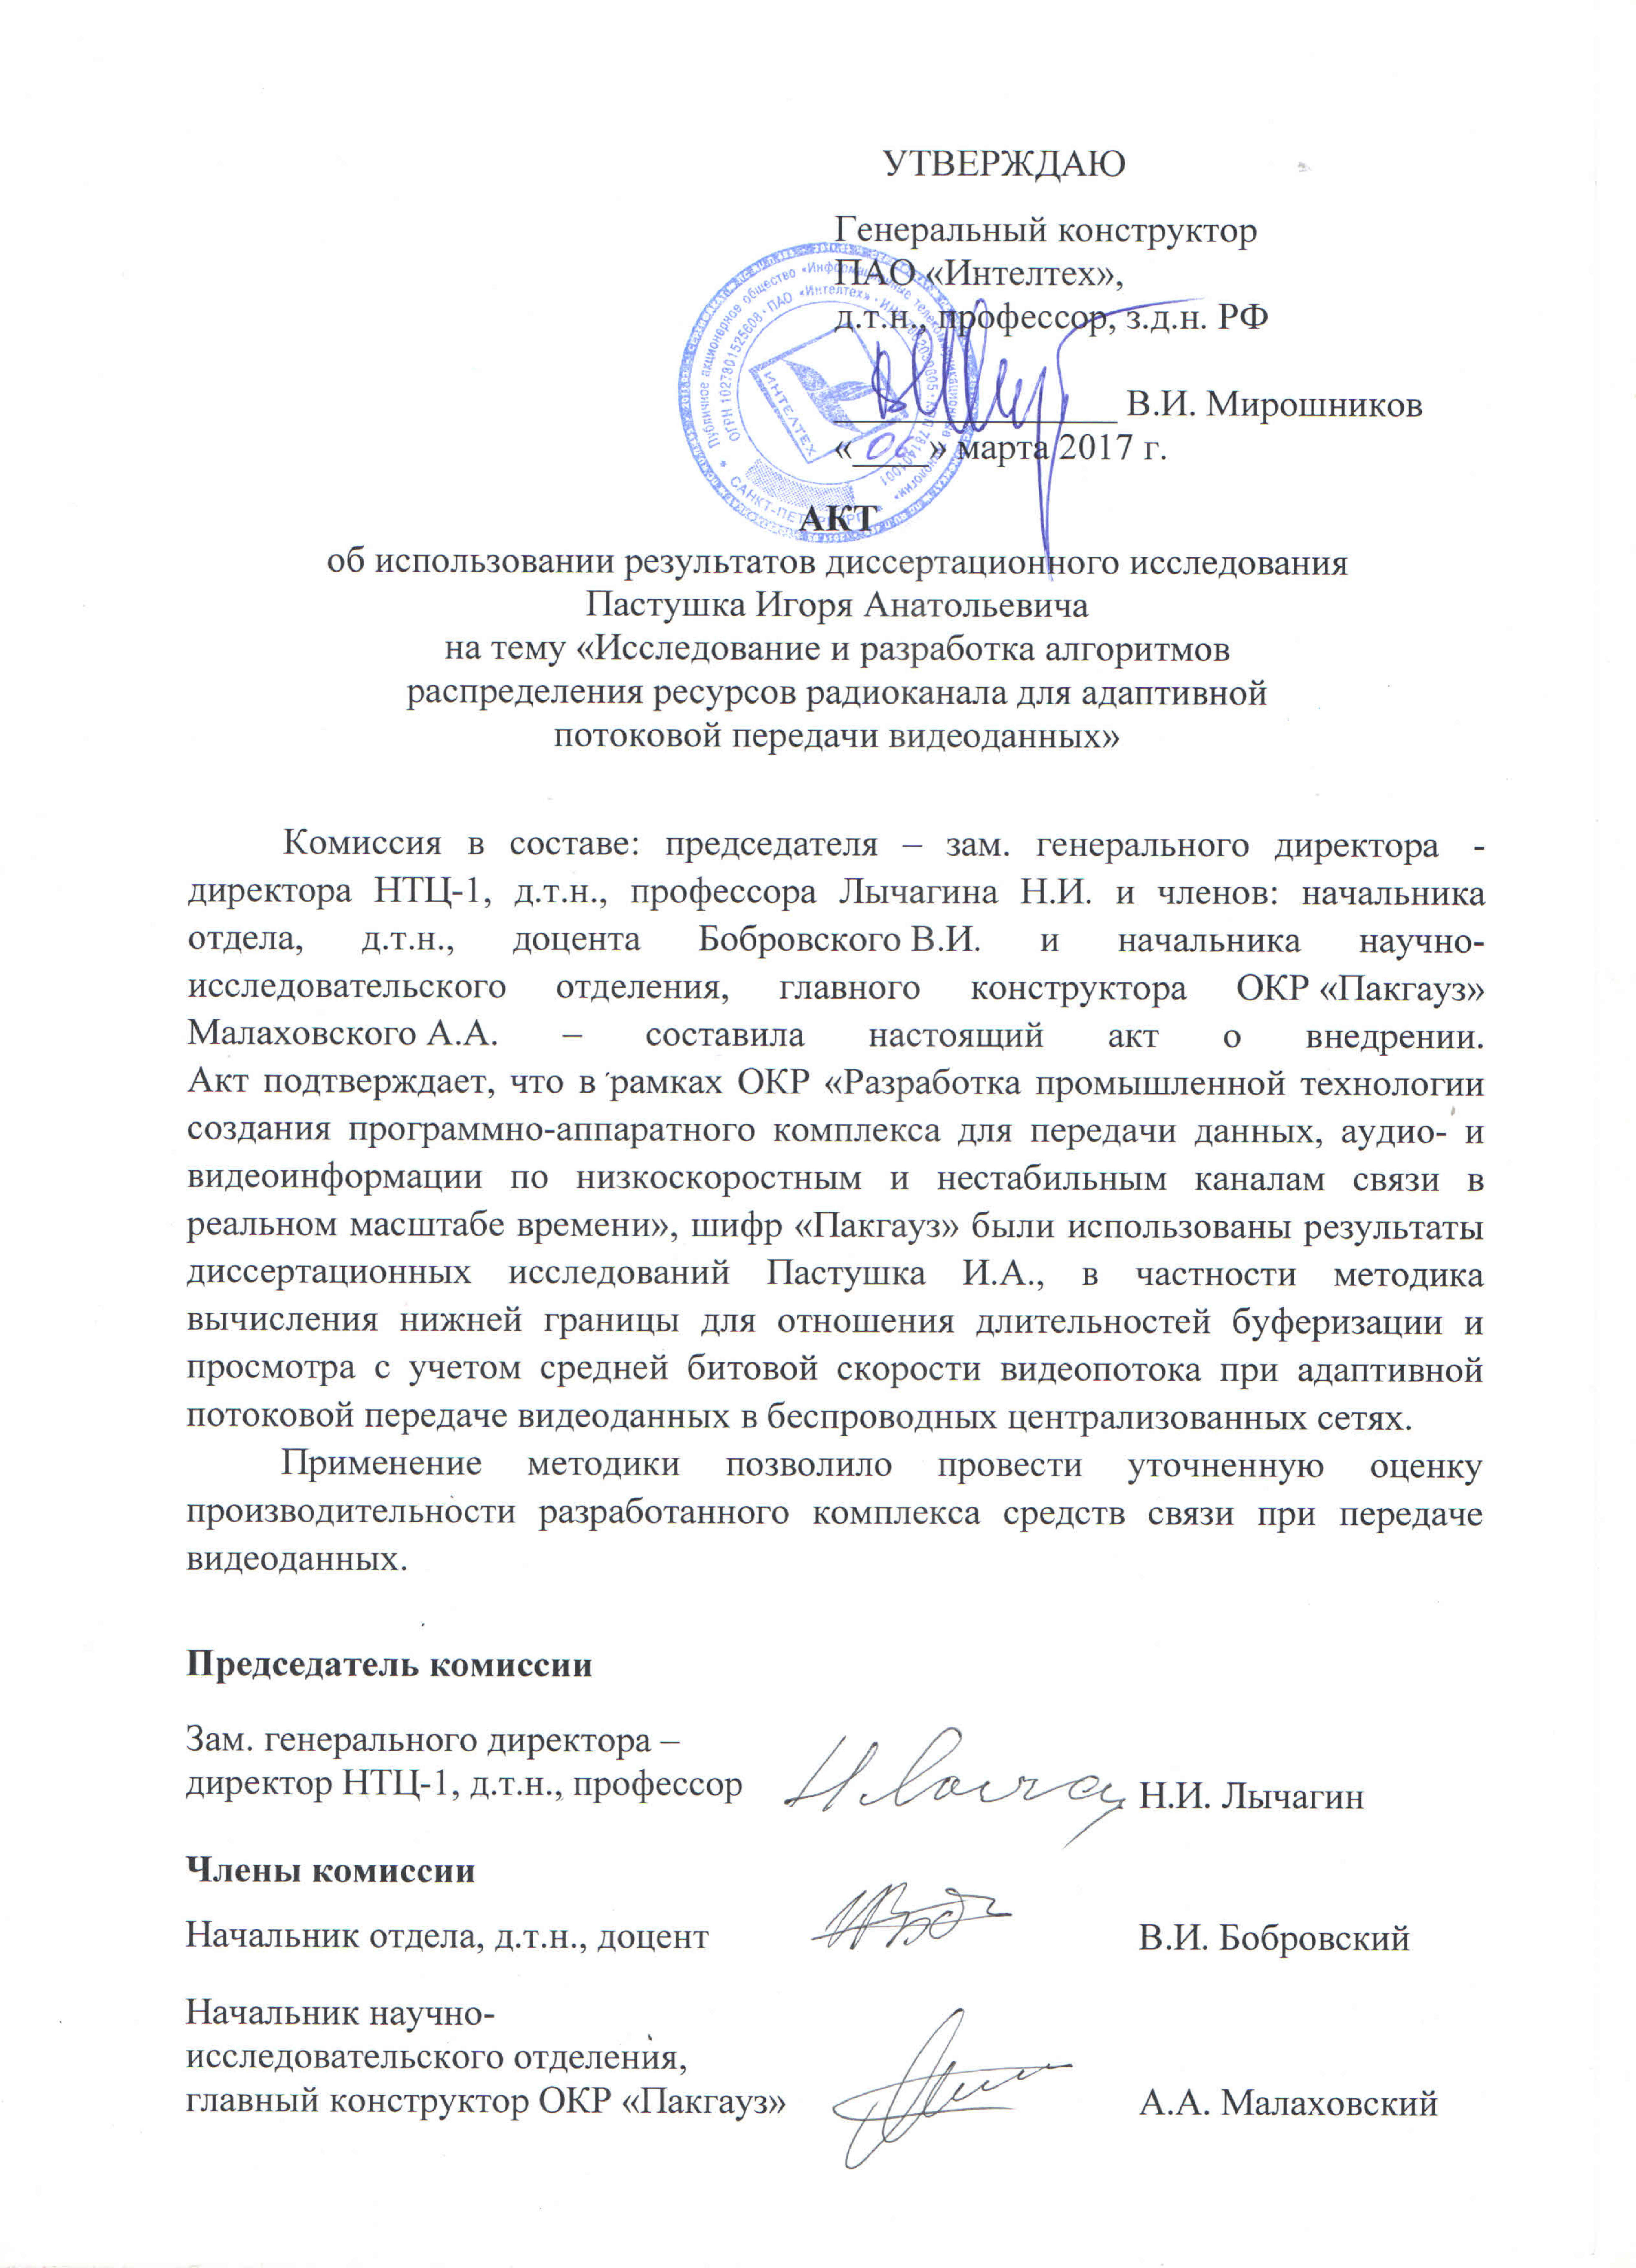
\includegraphics[width=1\textwidth,height=0.8\textheight]{appendix/Inteltech.pdf}
\end{center}
%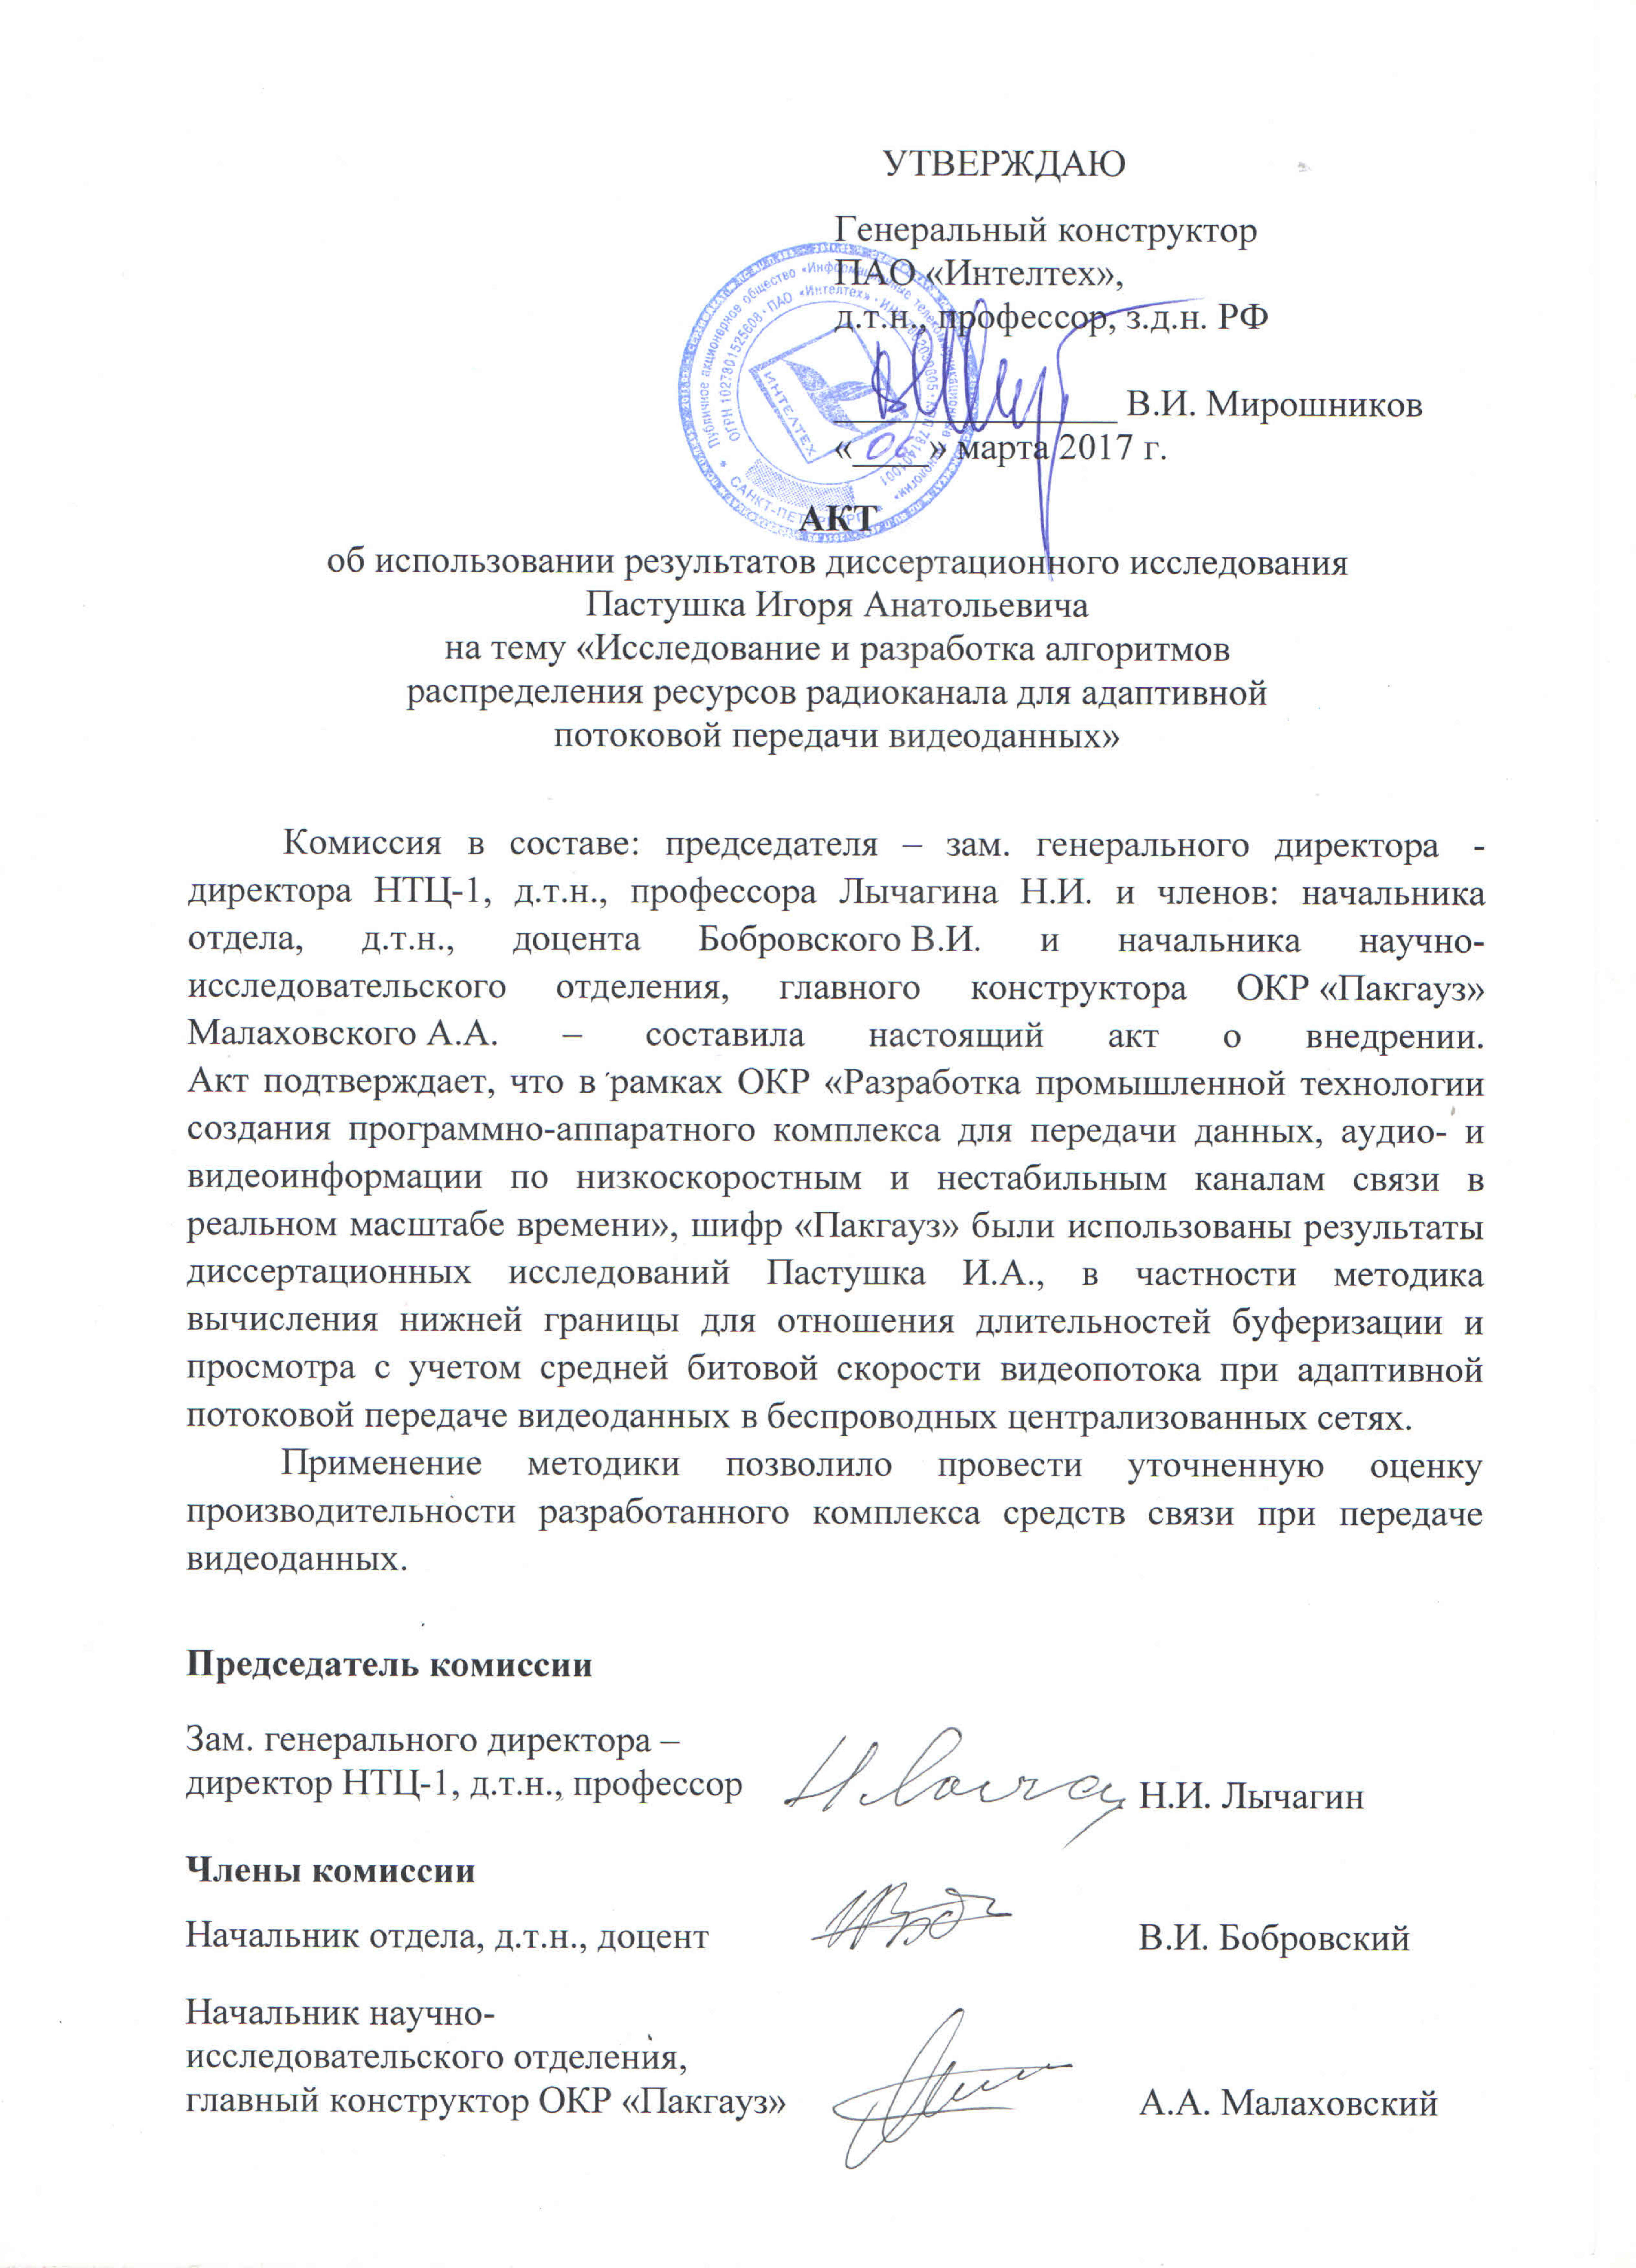
\includepdf[width=1.2\textwidth,height=0.7\textheight]{appendix/Inteltech.pdf}
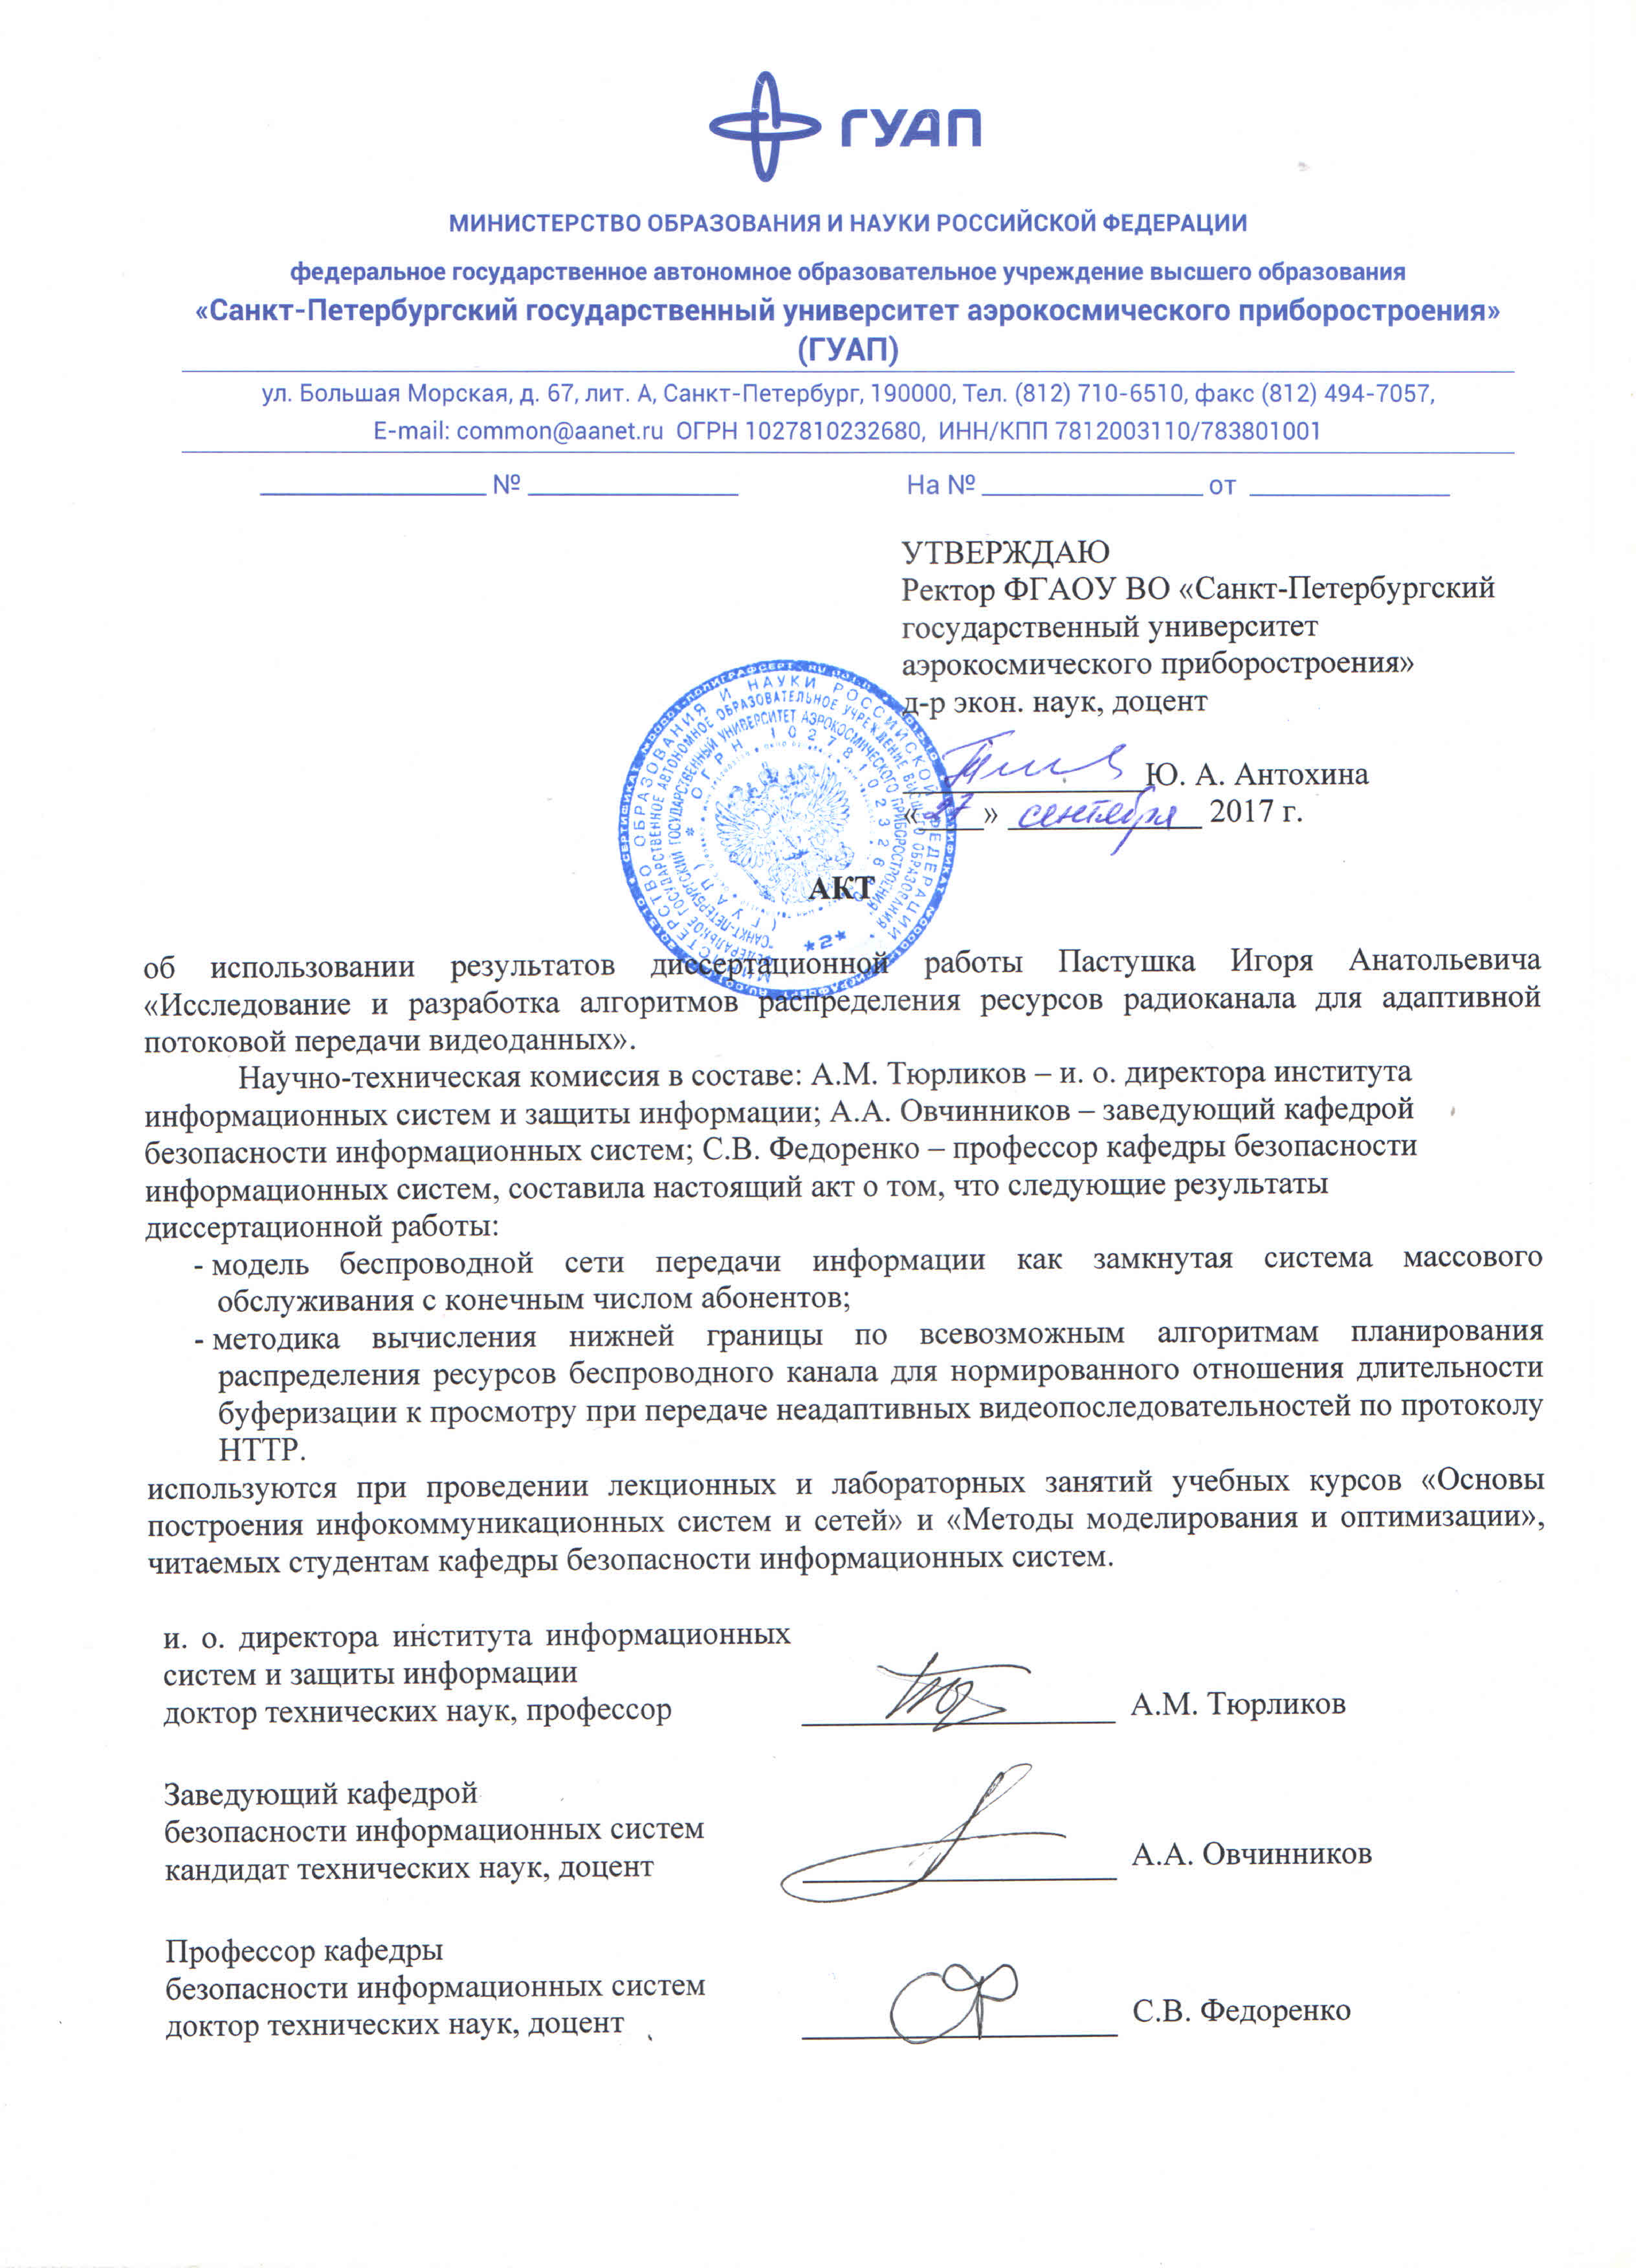
\includepdf{appendix/Act51.pdf}
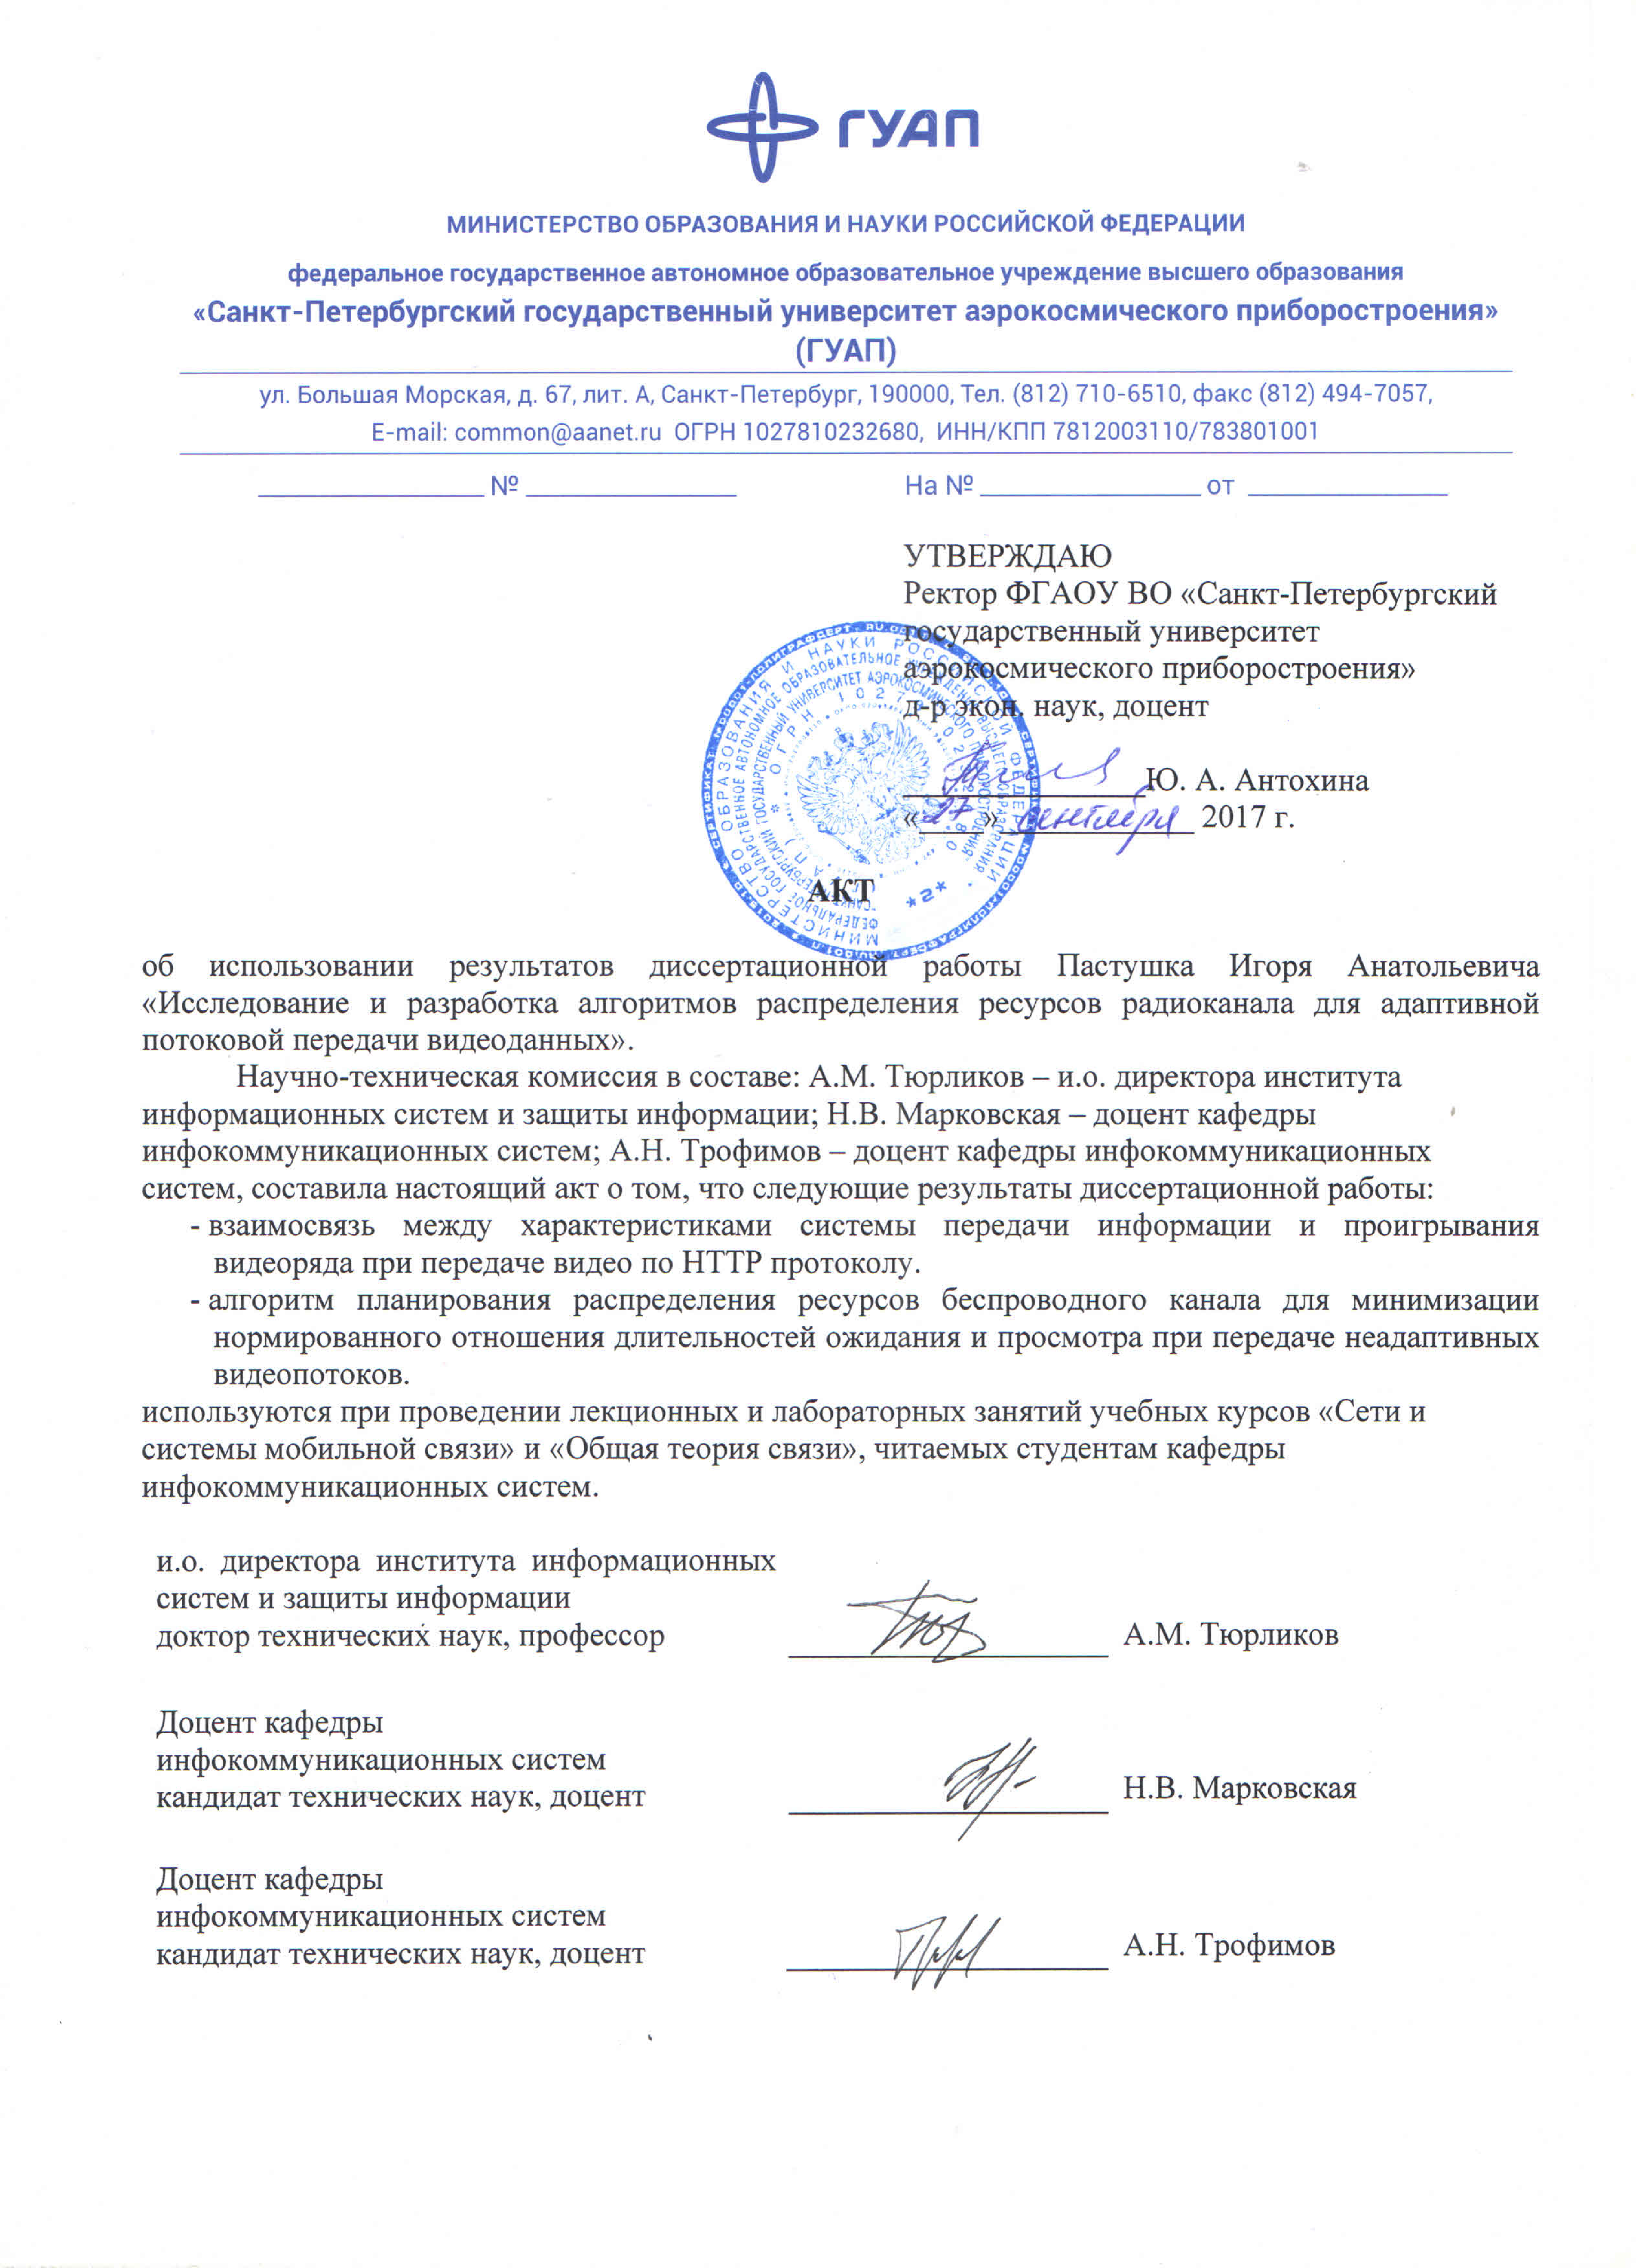
\includepdf{appendix/Act52.pdf}
%\chapter{Примеры вставки листингов программного кода} \label{AppendixA}
%
%Для крупных листингов есть два способа. Первый красивый, но в нём могут быть проблемы с поддержкой кириллицы (у вас может встречаться в комментариях и
%печатаемых сообщениях), он представлен на листинге~\ref{list:hwbeauty}.
%%\renewcommand\FBbskip{-20pt} % если хотим притянуть что-то к плавающему окружению из floatrow
%\begin{ListingEnv}[H]% буква H означает Here, ставим здесь,
%    % элементы, которые нежелательно разрывать обычно не ставят
%    % посреди страницы: вместо H используется t (top, сверху страницы),
%    % или b (bottom) или p (page, на отдельной странице)
%%    \captionsetup{format=tablenocaption}% должен стоять до самого caption
%%    \thisfloatsetup{\capposition=top}%
%    \caption{Программа “Hello, world” на \protect\cpp}
%    % далее метка для ссылки:
%    \label{list:hwbeauty}
%    % окружение учитывает пробелы и табляции и приеняет их в сответсвии с настройкми
%    \begin{lstlisting}[language={[ISO]C++}]
%	#include <iostream>
%	using namespace std;
%
%	int main() //кириллица в комментариях при xelatex и lualatex имеет проблемы с пробелами
%	{
%		cout << "Hello, world" << endl; //latin letters in commentaries
%		system("pause");
%		return 0;
%	}
%    \end{lstlisting}
%\end{ListingEnv}%
%Второй не такой красивый, но без ограничений (см.~листинг~\ref{list:hwplain}).
%\begin{ListingEnv}[H]
%    \begin{Verb}
%
%        #include <iostream>
%        using namespace std;
%
%        int main() //кириллица в комментариях
%        {
%            cout << "Привет, мир" << endl;
%        }
%    \end{Verb}
%    \caption{Программа “Hello, world” без подсветки}
%    \label{list:hwplain}
%\end{ListingEnv}
%
%Можно использовать первый для вставки небольших фрагментов
%внутри текста, а второй для вставки полного
%кода в приложении, если таковое имеется.
%
%Если нужно вставить совсем короткий пример кода (одна или две строки), то выделение  линейками и нумерация может смотреться чересчур громоздко. В таких случаях можно использовать окружения \texttt{lstlisting} или \texttt{Verb} без \texttt{ListingEnv}. Приведём такой пример с указанием языка программирования, отличного от заданного по умолчанию:
%\begin{lstlisting}[language=Haskell]
%fibs = 0 : 1 : zipWith (+) fibs (tail fibs)
%\end{lstlisting}
%Такое решение~--- со вставкой нумерованных листингов покрупнее
%и вставок без выделения для маленьких фрагментов~--- выбрано,
%например, в книге Эндрю Таненбаума и Тодда Остина по архитектуре
%%компьютера~\autocite{TanAus2013} (см.~рис.~\ref{fig:tan-aus}).
%
%Наконец, для оформления идентификаторов внутри строк
%(функция \lstinline{main} и тому подобное) используется
%\texttt{lstinline} или, самое простое, моноширинный текст
%(\texttt{\textbackslash texttt}).
%
%
%Пример~\ref{list:internal3}, иллюстрирующий подключение переопределённого языка. Может быть полезным, если подсветка кода работает криво. Без дополнительного окружения, с подписью и ссылкой, реализованной встроенным средством.
%\begin{lstlisting}[language={Renhanced},caption={Пример листинга c подписью собственными средствами},label={list:internal3}]
%## Caching the Inverse of a Matrix
%
%## Matrix inversion is usually a costly computation and there may be some
%## benefit to caching the inverse of a matrix rather than compute it repeatedly
%## This is a pair of functions that cache the inverse of a matrix.
%
%## makeCacheMatrix creates a special "matrix" object that can cache its inverse
%
%makeCacheMatrix <- function(x = matrix()) {#кириллица в комментариях при xelatex b lualatex имеет проблемы с пробелами
%    i <- NULL
%    set <- function(y) {
%        x <<- y
%        i <<- NULL
%    }
%    get <- function() x
%    setSolved <- function(solve) i <<- solve
%    getSolved <- function() i
%    list(set = set, get = get,
%    setSolved = setSolved,
%    getSolved = getSolved)
%
%}
%
%
%## cacheSolve computes the inverse of the special "matrix" returned by
%## makeCacheMatrix above. If the inverse has already been calculated (and the
%## matrix has not changed), then the cachesolve should retrieve the inverse from
%## the cache.
%
%cacheSolve <- function(x, ...) {
%    ## Return a matrix that is the inverse of 'x'
%    i <- x$getSolved()
%    if(!is.null(i)) {
%        message("getting cached data")
%        return(i)
%    }
%    data <- x$get()
%    i <- solve(data, ...)
%    x$setSolved(i)
%    i
%}
%\end{lstlisting}
%
%Листинг~\ref{list:external1} подгружается из внешнего файла. Приходится загружать без окружения дополнительного. Иначе по страницам не переносится.
%    \lstinputlisting[lastline=78,language={R},caption={Листинг из внешнего файла},label={list:external1}]{./listings/run_analysis.R}
%
%
%
%
%
%
%\chapter{Очень длинное название второго приложения, в котором продемонстрирована работа с длинными таблицами} \label{AppendixB}
%
% \section{Подраздел приложения}\label{AppendixB1}
%Вот размещается длинная таблица:
%\fontsize{10pt}{10pt}\selectfont
%\begin{longtable}[c]{|l|c|l|l|}
%% \caption{Описание входных файлов модели}\label{Namelists}
%%\\
% \hline
% %\multicolumn{4}{|c|}{\textbf{Файл puma\_namelist}}        \\ \hline
% Параметр & Умолч. & Тип & Описание               \\ \hline
%                                              \endfirsthead   \hline
% \multicolumn{4}{|c|}{\small\slshape (продолжение)}        \\ \hline
% Параметр & Умолч. & Тип & Описание               \\ \hline
%                                              \endhead        \hline
% \multicolumn{4}{|r|}{\small\slshape продолжение следует}  \\ \hline
%                                              \endfoot        \hline
%                                              \endlastfoot
% \multicolumn{4}{|l|}{\&INP}        \\ \hline
% kick & 1 & int & 0: инициализация без шума ($p_s = const$) \\
%      &   &     & 1: генерация белого шума                  \\
%      &   &     & 2: генерация белого шума симметрично относительно \\
%  & & & экватора    \\
% mars & 0 & int & 1: инициализация модели для планеты Марс     \\
% kick & 1 & int & 0: инициализация без шума ($p_s = const$) \\
%      &   &     & 1: генерация белого шума                  \\
%      &   &     & 2: генерация белого шума симметрично относительно \\
%  & & & экватора    \\
% mars & 0 & int & 1: инициализация модели для планеты Марс     \\
%kick & 1 & int & 0: инициализация без шума ($p_s = const$) \\
%      &   &     & 1: генерация белого шума                  \\
%      &   &     & 2: генерация белого шума симметрично относительно \\
%  & & & экватора    \\
% mars & 0 & int & 1: инициализация модели для планеты Марс     \\
%kick & 1 & int & 0: инициализация без шума ($p_s = const$) \\
%      &   &     & 1: генерация белого шума                  \\
%      &   &     & 2: генерация белого шума симметрично относительно \\
%  & & & экватора    \\
% mars & 0 & int & 1: инициализация модели для планеты Марс     \\
%kick & 1 & int & 0: инициализация без шума ($p_s = const$) \\
%      &   &     & 1: генерация белого шума                  \\
%      &   &     & 2: генерация белого шума симметрично относительно \\
%  & & & экватора    \\
% mars & 0 & int & 1: инициализация модели для планеты Марс     \\
%kick & 1 & int & 0: инициализация без шума ($p_s = const$) \\
%      &   &     & 1: генерация белого шума                  \\
%      &   &     & 2: генерация белого шума симметрично относительно \\
%  & & & экватора    \\
% mars & 0 & int & 1: инициализация модели для планеты Марс     \\
%kick & 1 & int & 0: инициализация без шума ($p_s = const$) \\
%      &   &     & 1: генерация белого шума                  \\
%      &   &     & 2: генерация белого шума симметрично относительно \\
%  & & & экватора    \\
% mars & 0 & int & 1: инициализация модели для планеты Марс     \\
%kick & 1 & int & 0: инициализация без шума ($p_s = const$) \\
%      &   &     & 1: генерация белого шума                  \\
%      &   &     & 2: генерация белого шума симметрично относительно \\
%  & & & экватора    \\
% mars & 0 & int & 1: инициализация модели для планеты Марс     \\
%kick & 1 & int & 0: инициализация без шума ($p_s = const$) \\
%      &   &     & 1: генерация белого шума                  \\
%      &   &     & 2: генерация белого шума симметрично относительно \\
%  & & & экватора    \\
% mars & 0 & int & 1: инициализация модели для планеты Марс     \\
%kick & 1 & int & 0: инициализация без шума ($p_s = const$) \\
%      &   &     & 1: генерация белого шума                  \\
%      &   &     & 2: генерация белого шума симметрично относительно \\
%  & & & экватора    \\
% mars & 0 & int & 1: инициализация модели для планеты Марс     \\
%kick & 1 & int & 0: инициализация без шума ($p_s = const$) \\
%      &   &     & 1: генерация белого шума                  \\
%      &   &     & 2: генерация белого шума симметрично относительно \\
%  & & & экватора    \\
% mars & 0 & int & 1: инициализация модели для планеты Марс     \\
%kick & 1 & int & 0: инициализация без шума ($p_s = const$) \\
%      &   &     & 1: генерация белого шума                  \\
%      &   &     & 2: генерация белого шума симметрично относительно \\
%  & & & экватора    \\
% mars & 0 & int & 1: инициализация модели для планеты Марс     \\
%kick & 1 & int & 0: инициализация без шума ($p_s = const$) \\
%      &   &     & 1: генерация белого шума                  \\
%      &   &     & 2: генерация белого шума симметрично относительно \\
%  & & & экватора    \\
% mars & 0 & int & 1: инициализация модели для планеты Марс     \\
%kick & 1 & int & 0: инициализация без шума ($p_s = const$) \\
%      &   &     & 1: генерация белого шума                  \\
%      &   &     & 2: генерация белого шума симметрично относительно \\
%  & & & экватора    \\
% mars & 0 & int & 1: инициализация модели для планеты Марс     \\
%kick & 1 & int & 0: инициализация без шума ($p_s = const$) \\
%      &   &     & 1: генерация белого шума                  \\
%      &   &     & 2: генерация белого шума симметрично относительно \\
%  & & & экватора    \\
% mars & 0 & int & 1: инициализация модели для планеты Марс     \\
% \hline
%  %& & & $\:$ \\
% \multicolumn{4}{|l|}{\&SURFPAR}        \\ \hline
%kick & 1 & int & 0: инициализация без шума ($p_s = const$) \\
%      &   &     & 1: генерация белого шума                  \\
%      &   &     & 2: генерация белого шума симметрично относительно \\
%  & & & экватора    \\
% mars & 0 & int & 1: инициализация модели для планеты Марс     \\
%kick & 1 & int & 0: инициализация без шума ($p_s = const$) \\
%      &   &     & 1: генерация белого шума                  \\
%      &   &     & 2: генерация белого шума симметрично относительно \\
%  & & & экватора    \\
% mars & 0 & int & 1: инициализация модели для планеты Марс     \\
%kick & 1 & int & 0: инициализация без шума ($p_s = const$) \\
%      &   &     & 1: генерация белого шума                  \\
%      &   &     & 2: генерация белого шума симметрично относительно \\
%  & & & экватора    \\
% mars & 0 & int & 1: инициализация модели для планеты Марс     \\
%kick & 1 & int & 0: инициализация без шума ($p_s = const$) \\
%      &   &     & 1: генерация белого шума                  \\
%      &   &     & 2: генерация белого шума симметрично относительно \\
%  & & & экватора    \\
% mars & 0 & int & 1: инициализация модели для планеты Марс     \\
%kick & 1 & int & 0: инициализация без шума ($p_s = const$) \\
%      &   &     & 1: генерация белого шума                  \\
%      &   &     & 2: генерация белого шума симметрично относительно \\
%  & & & экватора    \\
% mars & 0 & int & 1: инициализация модели для планеты Марс     \\
%kick & 1 & int & 0: инициализация без шума ($p_s = const$) \\
%      &   &     & 1: генерация белого шума                  \\
%      &   &     & 2: генерация белого шума симметрично относительно \\
%  & & & экватора    \\
% mars & 0 & int & 1: инициализация модели для планеты Марс     \\
%kick & 1 & int & 0: инициализация без шума ($p_s = const$) \\
%      &   &     & 1: генерация белого шума                  \\
%      &   &     & 2: генерация белого шума симметрично относительно \\
%  & & & экватора    \\
% mars & 0 & int & 1: инициализация модели для планеты Марс     \\
%kick & 1 & int & 0: инициализация без шума ($p_s = const$) \\
%      &   &     & 1: генерация белого шума                  \\
%      &   &     & 2: генерация белого шума симметрично относительно \\
%  & & & экватора    \\
% mars & 0 & int & 1: инициализация модели для планеты Марс     \\
%kick & 1 & int & 0: инициализация без шума ($p_s = const$) \\
%      &   &     & 1: генерация белого шума                  \\
%      &   &     & 2: генерация белого шума симметрично относительно \\
%  & & & экватора    \\
% mars & 0 & int & 1: инициализация модели для планеты Марс     \\
% \hline
%\end{longtable}
%
%\normalsize% возвращаем шрифт к нормальному
%\section{Ещё один подраздел приложения} \label{AppendixB2}
%
%Нужно больше подразделов приложения!
%
%Пример длинной таблицы с записью продолжения по ГОСТ 2.105
%
%    \centering
%	\small
%    \begin{longtable}[c]{|l|c|l|l|}
%	\caption{Наименование таблицы средней длины}%
%    \label{tbl:test5}% label всегда желательно идти после caption
%    \\
%    \hline
%     %\multicolumn{4}{|c|}{\textbf{Файл puma\_namelist}}        \\ \hline
%     Параметр & Умолч. & Тип & Описание               \\ \hline
%                                                  \endfirsthead
%%     \multicolumn{4}{|c|}{\small\slshape (продолжение)}        \\ \hline
% \captionsetup{format=tablenocaption,labelformat=continued}% должен стоять до самого caption
% \caption[]{} \\
%    \hline
%     Параметр & Умолч. & Тип & Описание               \\ \hline
%                                                  \endhead        \hline
%%     \multicolumn{4}{|r|}{\small\slshape продолжение следует}  \\
%%\hline
%                                                  \endfoot        \hline
%                                                  \endlastfoot
%     \multicolumn{4}{|l|}{\&INP}        \\ \hline
%     kick & 1 & int & 0: инициализация без шума ($p_s = const$) \\
%          &   &     & 1: генерация белого шума                  \\
%          &   &     & 2: генерация белого шума симметрично относительно \\
%      & & & экватора    \\
%     mars & 0 & int & 1: инициализация модели для планеты Марс     \\
%     kick & 1 & int & 0: инициализация без шума ($p_s = const$) \\
%          &   &     & 1: генерация белого шума                  \\
%          &   &     & 2: генерация белого шума симметрично относительно \\
%      & & & экватора    \\
%     mars & 0 & int & 1: инициализация модели для планеты Марс     \\
%    kick & 1 & int & 0: инициализация без шума ($p_s = const$) \\
%          &   &     & 1: генерация белого шума                  \\
%          &   &     & 2: генерация белого шума симметрично относительно \\
%      & & & экватора    \\
%     mars & 0 & int & 1: инициализация модели для планеты Марс     \\
%    kick & 1 & int & 0: инициализация без шума ($p_s = const$) \\
%          &   &     & 1: генерация белого шума                  \\
%          &   &     & 2: генерация белого шума симметрично относительно \\
%      & & & экватора    \\
%     mars & 0 & int & 1: инициализация модели для планеты Марс     \\
%    kick & 1 & int & 0: инициализация без шума ($p_s = const$) \\
%          &   &     & 1: генерация белого шума                  \\
%          &   &     & 2: генерация белого шума симметрично относительно \\
%      & & & экватора    \\
%     mars & 0 & int & 1: инициализация модели для планеты Марс     \\
%    kick & 1 & int & 0: инициализация без шума ($p_s = const$) \\
%          &   &     & 1: генерация белого шума                  \\
%          &   &     & 2: генерация белого шума симметрично относительно \\
%      & & & экватора    \\
%     mars & 0 & int & 1: инициализация модели для планеты Марс     \\
%    kick & 1 & int & 0: инициализация без шума ($p_s = const$) \\
%          &   &     & 1: генерация белого шума                  \\
%          &   &     & 2: генерация белого шума симметрично относительно \\
%      & & & экватора    \\
%     mars & 0 & int & 1: инициализация модели для планеты Марс     \\
%    kick & 1 & int & 0: инициализация без шума ($p_s = const$) \\
%          &   &     & 1: генерация белого шума                  \\
%          &   &     & 2: генерация белого шума симметрично относительно \\
%      & & & экватора    \\
%     mars & 0 & int & 1: инициализация модели для планеты Марс     \\
%    kick & 1 & int & 0: инициализация без шума ($p_s = const$) \\
%          &   &     & 1: генерация белого шума                  \\
%          &   &     & 2: генерация белого шума симметрично относительно \\
%      & & & экватора    \\
%     mars & 0 & int & 1: инициализация модели для планеты Марс     \\
%    kick & 1 & int & 0: инициализация без шума ($p_s = const$) \\
%          &   &     & 1: генерация белого шума                  \\
%          &   &     & 2: генерация белого шума симметрично относительно \\
%      & & & экватора    \\
%     mars & 0 & int & 1: инициализация модели для планеты Марс     \\
%    kick & 1 & int & 0: инициализация без шума ($p_s = const$) \\
%          &   &     & 1: генерация белого шума                  \\
%          &   &     & 2: генерация белого шума симметрично относительно \\
%      & & & экватора    \\
%     mars & 0 & int & 1: инициализация модели для планеты Марс     \\
%    kick & 1 & int & 0: инициализация без шума ($p_s = const$) \\
%          &   &     & 1: генерация белого шума                  \\
%          &   &     & 2: генерация белого шума симметрично относительно \\
%      & & & экватора    \\
%     mars & 0 & int & 1: инициализация модели для планеты Марс     \\
%    kick & 1 & int & 0: инициализация без шума ($p_s = const$) \\
%          &   &     & 1: генерация белого шума                  \\
%          &   &     & 2: генерация белого шума симметрично относительно \\
%      & & & экватора    \\
%     mars & 0 & int & 1: инициализация модели для планеты Марс     \\
%    kick & 1 & int & 0: инициализация без шума ($p_s = const$) \\
%          &   &     & 1: генерация белого шума                  \\
%          &   &     & 2: генерация белого шума симметрично относительно \\
%      & & & экватора    \\
%     mars & 0 & int & 1: инициализация модели для планеты Марс     \\
%    kick & 1 & int & 0: инициализация без шума ($p_s = const$) \\
%          &   &     & 1: генерация белого шума                  \\
%          &   &     & 2: генерация белого шума симметрично относительно \\
%      & & & экватора    \\
%     mars & 0 & int & 1: инициализация модели для планеты Марс     \\
%     \hline
%      %& & & $\:$ \\
%     \multicolumn{4}{|l|}{\&SURFPAR}        \\ \hline
%    kick & 1 & int & 0: инициализация без шума ($p_s = const$) \\
%          &   &     & 1: генерация белого шума                  \\
%          &   &     & 2: генерация белого шума симметрично относительно \\
%      & & & экватора    \\
%     mars & 0 & int & 1: инициализация модели для планеты Марс     \\
%    kick & 1 & int & 0: инициализация без шума ($p_s = const$) \\
%          &   &     & 1: генерация белого шума                  \\
%          &   &     & 2: генерация белого шума симметрично относительно \\
%      & & & экватора    \\
%     mars & 0 & int & 1: инициализация модели для планеты Марс     \\
%    kick & 1 & int & 0: инициализация без шума ($p_s = const$) \\
%          &   &     & 1: генерация белого шума                  \\
%          &   &     & 2: генерация белого шума симметрично относительно \\
%      & & & экватора    \\
%     mars & 0 & int & 1: инициализация модели для планеты Марс     \\
%    kick & 1 & int & 0: инициализация без шума ($p_s = const$) \\
%          &   &     & 1: генерация белого шума                  \\
%          &   &     & 2: генерация белого шума симметрично относительно \\
%      & & & экватора    \\
%     mars & 0 & int & 1: инициализация модели для планеты Марс     \\
%    kick & 1 & int & 0: инициализация без шума ($p_s = const$) \\
%          &   &     & 1: генерация белого шума                  \\
%          &   &     & 2: генерация белого шума симметрично относительно \\
%      & & & экватора    \\
%     mars & 0 & int & 1: инициализация модели для планеты Марс     \\
%    kick & 1 & int & 0: инициализация без шума ($p_s = const$) \\
%          &   &     & 1: генерация белого шума                  \\
%          &   &     & 2: генерация белого шума симметрично относительно \\
%      & & & экватора    \\
%     mars & 0 & int & 1: инициализация модели для планеты Марс     \\
%    kick & 1 & int & 0: инициализация без шума ($p_s = const$) \\
%          &   &     & 1: генерация белого шума                  \\
%          &   &     & 2: генерация белого шума симметрично относительно \\
%      & & & экватора    \\
%     mars & 0 & int & 1: инициализация модели для планеты Марс     \\
%    kick & 1 & int & 0: инициализация без шума ($p_s = const$) \\
%          &   &     & 1: генерация белого шума                  \\
%          &   &     & 2: генерация белого шума симметрично относительно \\
%      & & & экватора    \\
%     mars & 0 & int & 1: инициализация модели для планеты Марс     \\
%    kick & 1 & int & 0: инициализация без шума ($p_s = const$) \\
%          &   &     & 1: генерация белого шума                  \\
%          &   &     & 2: генерация белого шума симметрично относительно \\
%      & & & экватора    \\
%     mars & 0 & int & 1: инициализация модели для планеты Марс     \\
%     \hline
%    \end{longtable}
%\normalsize% возвращаем шрифт к нормальному
%\section{Очередной подраздел приложения} \label{AppendixB3}
%
%Нужно больше подразделов приложения!
%
%\section{И ещё один подраздел приложения} \label{AppendixB4}
%
%Нужно больше подразделов приложения!

        % Приложения

\end{document}
